\part{Números enteros y aritmética} 

\chapter[Números Enteros]{Números Enteros}\label{cap.numeros_enteros}

\begin{section}{Aritmética}\label{1.1}
 Todo lector de este apunte conoce los \textit{enteros}. En una etapa muy temprana de nuestras vidas conocemos los números enteros positivos o ``números naturales'' $$1,2,3,4,5,\ldots$$ Más adelante introducimos el $0$ (cero), y los enteros negativos $$ -1,-2,-3,-4,-5,\ldots $$ 

En este curso no nos preocupamos demasiado por el significado lógico y filosófico de estos objetos, pero necesitamos saber las propiedades que se supone que tienen. Si todos parten de las mismas suposiciones entonces todos llegarán a los mismos resultados. Estos supuestos son los llamados axio\-mas.

El punto de vista adoptado en este apunte es el señalado antes. Aceptamos sin reparo que existe un conjunto de objetos llamados \textit{enteros} conteniendo los enteros positivos y los negativos, y el cero, familiares en nuestra temprana educación y experiencia. El conjunto de enteros se denotará por el símbolo especial ${\mathbb Z}$. Las propiedades de ${\mathbb Z}$ serán dadas por una lista de axiomas, a partir de las cuales seremos capaces de deducir todos los resultados sobre números enteros que necesitaremos en las cuestiones subsiguientes. Empezaremos listando aquellos axiomas que tratan la suma y la multiplicación.

Adoptaremos las notaciones usuales $a+b$ para la suma de dos enteros $a$ y $b$, y $a \times b$ (frecuentemente $a \cdot b$ o solo $ab$) para su producto. Pensamos en $+$ y $\times$ como \textit{operaciones} que a un par de enteros $a$ y $b$ les hacen corresponder un entero $a+b$ y otro $a\times b$. El hecho de que $a \times b$ y $a+b$ son enteros, y no algún objeto extra\~no como elefantes, es nuestra primera suposición axioma (\textbf{I1}).     

En la siguiente lista de axiomas $a$, $b$, $c$ denotan enteros arbitrarios, y $0$ y $1$ denotan enteros especiales que cumplen las propiedades especificadas más abajo.

\begin{enumerate}
\item[\textbf{I1)}] $a+b$ y $ab$ pertenecen a ${\mathbb Z}$.
\item[\textbf{I2)}] {\em Conmutatividad.}\, $a+b = b+a$;\qquad $ab=ba$. 
\item[\textbf{I3)}] {\em Asociatividad.}\, $(a+b)+c = a+(b+c)$;\qquad $(ab)c = a(bc)$. 
\item[\textbf{I4)}] {\em Existencia de elemento neutro.}\, Existen números $0$, $1 \in \mathbb Z$ con $0\not=1$ tal que $a+0=a$;\qquad $a1=a$. 
\item[\textbf{I5)}] {\em Distributividad.}\, $a(b+c)=ab+ac$. 
\item[\textbf{I6)}] {\em Existencia del inverso aditivo, también llamado opuesto.}\, Por cada $a$ en ${\mathbb Z}$ existe un único entero $-a$ en ${\mathbb Z}$ tal que $a+(-a)=0$. 
\item[\textbf{I7)}] {\em Cancelación.}\, Si $a$ es distinto de $0$ y $ab=ac$, entonces $b=c$. 
\end{enumerate}


Debido a la ley de asociatividad para la suma axioma (\textbf{I3}) $(a+b)+c$ es igual a $a+(b+c)$ y por lo tanto podemos eliminar los paréntesis sin ambigüedad. Es decir, denotamos
$$
a+b+c := (a+b)+c = a+(b+c).
$$
De forma análoga, usaremos la notación
$$
abc = (ab)c = a(bc).
$$
Debido a la ley de conmutatividad axioma (\textbf{I2}), es claro que  del axioma (\textbf{I4}) se deduce que  $0+a=a+0=a$ y $1a = a1=a$. Análogamente,  por  (\textbf{I2}) e  (\textbf{I6}) obtenemos que  $-a+a =    a+(-a)=0$.

Una propiedad que debemos mencionar es la siguiente: si $a,b, c \in \mathbb Z$  y $a=b$, entonces $a+c = b+c$ y $ac = bc$. Esto se debe a que la suma y el producto son operaciones que, como acabamos de decir, toman un par de enteros y  devuelven otro entero. Si $a=b$, entonces el  par $a,c$ es igual al par $b,c$ y por lo tanto devuelven la misma suma y el mismo producto. Esta propiedad no es un axioma, sino  una mera aplicación de la lógica formal. 
  
Todos los axiomas corresponden a propiedades familiares de los  enteros que aprendemos en distintos niveles de nuestra educación  matemática. De ellas pueden deducirse la mayoría de las reglas  aritméticas comunes de los enteros como en el siguiente ejemplo.

\begin{ejemplo}\label{Ej.opuesto_opuesto} Demostremos que, para todo $n$ entero, el opuesto de $-n$ es $n$, es decir que 
$$-(-n) = n.$$ 
\end{ejemplo}
\begin{proof} El axioma (\textbf{I6}) nos dice que $-(-n)$ es el único número que sumado a $-n$, da cero.  Por lo tanto, para demostrar que $-(-n) = n$ basta ver que $(-n)+n=0$. Esto se cumple puesto que 
\begin{alignat*}2
(-n)+n&=n+(-n) &\qquad &\text{axioma (\textbf{I2})} \\
&=0&\qquad &\text{axioma (\textbf{I6})}
\end{alignat*}
Por lo tanto  $(-n)+n=0$.
\end{proof}

Como ya dijimos, los números enteros vienen provistos con dos operaciones fundamentales, la suma y la multiplicación.
A continuación definimos la resta o sustracción. 

\begin{definicion} Si $a,b\in\mathbb{Z}$ definimos $a-b$ como la suma de $a$ más el opuesto de $b$, es decir que  $a-b=a+(-b)$ por definición.  
\end{definicion}

Ahora demostremos una propiedad básica de la resta.

\begin{ejemplo*} Demostremos que para dos enteros $m$ y $n$ cualesquiera
$$m-(-n) = m+n.$$ 
\end{ejemplo*}
\begin{proof} Por la definición de sustracción, $m-(-n)$ es la suma $m+(-(-n))$, es decir 
$$m-(-n)=m+(-(-n)).$$ 
Por el ejemplo \ref{Ej.opuesto_opuesto} sabemos que $-(-n)=n$ y por lo tanto $m-(-n)=m+(-(-n))=m+n$.
\end{proof}

Tanto formalismo, como el usado en las  demostraciones realizadas en el ejemplo anterior, puede ser tedioso, pero nos permiten comenzar a comprender la estructura de una demostración formal. 



\begin{ejemplo*} Supongamos que existen dos enteros $0$ y $0'$ ambos cumpliendo el  axioma (\textbf{I4}), esto es
$$
a+0= a, \qquad a+0'=a
$$
para todo $a$ de $\mathbb Z$. 
\end{ejemplo*}
\begin{proof}
\begin{alignat*}2
0 &= 0 + 0'&\qquad &\text{axioma (\textbf{I4}) aplicado a $0$ y con $0'$ como neutro} \\
&=0'+0&\qquad &\text{axioma (\textbf{I2})}\\
&= 0' &\qquad &\text{axioma (\textbf{I4}) aplicado a $0'$ y con $0$ como neutro}.
\end{alignat*}
\end{proof}


El ejemplo anterior nos demuestra que hay un único elemento elemento que cumple el axioma (\textbf{I4}) en lo que respecta a la suma. A este elemento lo denotamos $0$ y lo denominamos el {\em elemento neutro de la suma}. Lo mismo podemos probar con el elemento neutro respecto al producto (ver ejercicio \ref{ej-elem-neutro-prod}),  es decir hay un único elemento,  denotado 1, que satisface el axioma (\textbf{I4}) en lo que se refiere al producto. A  este elemento lo llamamos el {\em elemento neutro del producto}.  

\begin{ejemplo*} (Regla de los signos) Veamos que  si $a,b \in \mathbb Z$ entonces
$$
(-a)(-b) = ab ,\qquad a(-b) = (-a)b = -(ab).
$$
\end{ejemplo*}
\begin{proof}
Veremos que  $a(-b) = -(ab)$. Los otros casos se dejan como ejercicio para el lector.

Una forma de demostrar este caso es  observando que $-(ab)$ es el inverso aditivo de $ab$ y comprobando que $a(-b)$ es también inverso aditivo de $ab$. Luego, por unicidad del inverso aditivo, de deduce que $a(-b) = -(ab)$. 
\begin{alignat*}2
ab + a(-b) &=a(b-b) &\qquad &\text{axioma (\textbf{I5})} \\
&=a0 &\qquad &\text{axioma (\textbf{I4})}\\
&= 0 &\qquad &\text{ejercicio \ref{ej0a}}.
\end{alignat*}
Es decir $a(-b)$ es el inverso aditivo de $ab$, luego por la unicidad del inverso aditivo axioma (\textbf{I6}), $a(-b)=-(ab)$.
\end{proof}


Algunos resultados similares pueden encontrarse en los siguientes ejercicios. Como aún no tenemos todos los axiomas correspondientes a los enteros, los resultados no son particularmente interesantes, pero lo que importa es recordar que pueden ser probados sobre la base única de los axiomas.

%\begin{subsection}{Ejercicios}
\subsection*{$\S$ Ejercicios}
%\addcontentsline{toc}{subsection}{Ejercicios}

\begin{enumerate}
\item Demostrar la regla $(a+b)c=ac+bc$, explicando cada paso.

\item Como siempre $x^2$ denota $xx$. Demostrar que dados dos enteros $a$ y $b$ tal que $a+b \not=0$, entonces existe un único $c$ tal que $(a+b)c=
a^2 - b^2$.

\item \label{ej-elem-neutro-prod}Probar que hay un único elemento neutro del producto.

\item \label{ej0a}
La siguiente es una demostración de la fórmula $0x=0$ usando solo los axiomas planteados antes. Escribir la demostración completa, explicando que axioma es usado en cada paso.
$$\begin{aligned}
0x &= (0+0)x &\qquad &\mbox{axioma (.....)}\\  
&=0x+0x. &\qquad &\mbox{axioma (.....)}
\end{aligned}$$
Luego $0x =0x+0x$. Sumando $-0x$ a ambos miembros de la igualdad, obtenemos 
$$\begin{aligned}
0x +(-0x) &= 0x+0x+(-0x) &\qquad &\mbox{(usando lógica formal)}\\  
0 &= 0x+0 &\qquad &\mbox{axioma (.....), 2 veces}\\  
0 &=0x. &\qquad &\mbox{axioma (.....)}
\end{aligned}$$
\end{enumerate}
%\end{subsection}

\end{section}



\begin{section}{Ordenando los enteros}\label{1.2}

El orden natural de los enteros es tan importante como sus propiedades aritméticas. Desde el comienzo aprendemos los números en el orden $1, 2, 3, 4, 5,$ y el hecho de que $4$ es ``mayor'' que $3$ se convierte en algo de importancia práctica para nosotros. Expresamos esta idea formalmente diciendo que existe una relación que indicamos ``$<$'' ($a < b$ se lee: $a$ es menor que $b$ o también $b$ es mayor que $a$). 

Solo cuatro axiomas se necesitan para especificar las propiedades básicas del símbolo $<$ , y ellos son listados en lo que sigue. La numeración de los axiomas se continúa de la sección \ref{1.1}. Como antes, $a$, $b$ y $c$ denotan enteros arbitrarios.

\begin{enumerate}
\item[\textbf{I8)}] {\em Ley de tricotomía.}\, Vale una y sólo una de las relaciones
siguientes:
$$
a<b, \qquad a = b, \qquad b < a.
$$
\item[\textbf{I9)}] {\em Ley transitiva.}\, Si $a< b$ y $b < c$, entonces $a<c$.
\item[\textbf{I10)}] {\em Compatibilidad de la suma con el orden.}\, Si $a < b$, entonces $a+c < b+c$. 
\item[\textbf{I11)}] {\em Compatibilidad del producto con el orden.}\, Si $a< b$ y $0< c$, entonces $ac < bc$. 
\end{enumerate}


Esta claro que podemos definir los otros símbolos de orden $>$, $\le$ y $\ge$, en términos de los símbolos $<$ e $=$. Diremos que $m>n$ si  $n<m$, diremos que $m \le n$ si $m<n$ o $m=n$. Finalmente, diremos que $m \ge n$ si $m > n$ o $m=n$.  Es importante notar que el  axioma (\textbf{I11}) tiene una versión valedera para estos nuevos símbolos.
\begin{enumerate}[label=\textit{\alph*)}]
\item \textbf{($>$)} Si $a > b$ y $c>0$, entonces $ac > bc$.
\item \textbf{($\le$)} Si $a \le b$ y $0 \le c$, entonces $ac \le bc$.
\item \textbf{($\ge$)} Si $a\ge b$ y $c\ge 0$, entonces $ac \ge bc$.
\end{enumerate}
Usando las definiciones de $\ge$, $<$, $>$ y el axioma (\textbf{I11}) original es muy sencillo demostrar estas variantes. Por otro lado,

\begin{proposicion}\label{prop-compatibilidad-negativa}
    Sean $a, b, c \in \Z$.  
    \begin{enumerate}[label=\textit{\alph*)}]
        \item\label{it.cmenor0} Si $c < 0$, entonces $0 < -c$.
        \item\label{it.amenorb} Si $a< b$ y $c< 0$, entonces $ac > bc$. 
    \end{enumerate}
\end{proposicion}
\begin{proof}[Demostración (*)] {${}^{}$}
    
    \ref{it.cmenor0} Sumando $-c$ a ambos miembros de la desigualdad $c < 0$, obtenemos $c + (-c) < 0 + (-c)$ (compatibilidad de la suma con la relación de orden). Por los axiomas de inverso aditivo y elemento neutro, la expresión se reduce a $0 < -c$.
    
    \ref{it.amenorb} Como $a < b$, si sumamos a ambos miembros de la desigualdad $-a -b$, por la compatibilidad  de la suma con $<$, obtenemos $a -a -b < b -a -b$ y por la aplicación reiterada de los axiomas de inverso aditivo y elemento neutro  obtenemos $-b < -a$. Por a) sabemos que $0< -c$, por lo tanto, por \textbf{I11)}, $(-b)(-c) < (-a)(-c)$. Aplicando la regla de los signos obtenemos $bc < ac$ y por lo tanto $ac > bc$.

\end{proof}

Ya hemos usado (en axioma \textbf{I4}) el símbolo $\not=$ que denota  ``{\em no} es igual a '' o bien ``es distinto a''.   En  general, cuando tachemos un símbolo, estamos indicando la negación de la relación que define. Por ejemplo, $a\not< b$ denota ``$a$ {\em no} es menor que $b$''. 

\begin{observacion*} Demostremos que  $a\not< b$ es equivalente a $a\ge b$: por la ley de tricotomía axioma (\textbf{I8}) tenemos que solo vale una y solo una de las siguientes afirmaciones
$$
a<b, \qquad a = b, \qquad b < a.
$$
Como  $a\not< b$, entonces vale una de las dos afirmaciones siguientes, $a=b$ o $b<a$, es decir  vale que $a \ge b$. De forma análoga se prueba que $a\not\le b$ si  y sólo si $a>b$, $a\not> b$ si  y sólo si $a \le b$ y $a\not\ge b$ si  y sólo si $a<b$.

\end{observacion*}


\begin{ejemplo}\label{relaciondeorden}
Demostremos las siguiente propiedades de $\le$. Sean  $a$, $b$ y $c$  enteros arbitrarios,  entonces
\begin{enumerate}
\item[\textbf{O1)}] {\em Reflexividad.}\, $a \le a$.
\item[\textbf{O2)}] {\em Antisimetría.}\, Si $a \le b$ y $b \le a$, entonces $a=b$.
\item[\textbf{O3)}] {\em Transitividad.}\, Si $a\le b$ y $b\le c$, entonces $a \le c$.
\end{enumerate}
\begin{proof}
\
    
(\textbf{O1}) Como $a=a$, tenemos entonces que $a \le a$ (por definición de $\le$).


(\textbf{O2}) Como $a \le b$, tenemos que $a<b$ o bien $a=b$ (por tricotomía no pueden valer ambas). Si ocurriera que $a<b$, por la observación anterior, tendríamos que $a\not\ge b$, es decir $b\not\le a$, lo cual es absurdo pues una de nuestras hipótesis es,  justamente, lo contrario:  $b \le a$.  Es decir, la única posibilidad que queda es que $a=b$.     

%\vskip .2cm
(\textbf{O3}) Como $a\le b$, entonces $a <b$ o bien $a=b$. Como $b\le c$, entonces $b<c$ o bien $b=c$. Para hacer la demostración, debemos pensar en todas las posibles combinaciones de estas afirmaciones:
\begin{itemize}
    \item $a<b$ y $b<c$. Es este caso, por  (\textbf{I9}), $a<c$. Luego $a\le c$.
    
    \item $a<b$ y $b=c$. Luego $a<c$ y eso implica que $a\le c$.
    
    \item $a=b$ y $b<c$. Luego $a<c$ y eso implica que $a\le c$.
    
    \item $a=b$ y $b=c$. Es claro entonces que $a=c$, lo cual implica que $a\le c$.
\end{itemize}    
\end{proof}
\end{ejemplo}

Una relación que satisfaga las tres propiedades anteriores (reflexividad, antisimetría y transitividad) es llamada {\em una relación de orden}. Observar que $<$ {\em no} es una relación de orden, en el sentido de la definición anterior. 

A primera vista podría parecer que ya tenemos todas las propiedades que necesitamos de $\mathbb Z$, pero, sorprendentemente, aún falta un axioma de vital importancia. Supongamos que $X$ es un subconjunto de $\mathbb Z$; entonces diremos que el entero $b$ es una {\em cota inferior}\index{cota inferior} de $X$ si
$$
b\le x \qquad \text{ para todo } \ x \in X.
$$
Algunos subconjuntos no tienen cotas inferiores: por ejemplo, el conjunto de los enteros negativos $-1, -2, -3, \ldots$, claramente no tiene cota inferior. Por otro lado, el conjunto $S$ denotado por los números resaltados en la Fig. \ref{f1.1} tiene muchas cotas inferiores. Una mirada rápida nos dice que $-9$ por ejemplo es una cota inferior, mientras que una inspección más minuciosa revela que $-7$ es la ``mejor'' cota inferior, pues en realidad pertenece a $S$. En general, una cota inferior de un conjunto $X$ que es a su vez es un elemento de $X$, es conocido como el {\em mínimo}\index{mínimo} de X.

%\vskip .3cm


\begin{figure}[ht]
$$
-10, -9, -8, \mathbf{-7}, \mathbf{-6}, -5, -4, \mathbf{-3}, -2, -1, 0, \mathbf{1}, \mathbf{2}, \mathbf{3}, 
4, 5, 6, 7, 8, 9, 10
$$
\caption{El mínimo de $S$ es $-7$.}\label{f1.1}
\end{figure}
%\vskip .3cm


Nuestro último axioma para $\mathbb Z$ afirma algo que es (aparentemente) una propiedad obvia.

\begin{enumerate}
\item[\textbf{I12)}] Si $X$ es un subconjunto de $\mathbb Z$ que no es vacío y tiene una cota inferior, entonces $X$ tiene un mínimo.
\end{enumerate}

El axioma (\textbf{I12}) es conocido como el {\em axioma del buen orden}\index{axioma del buen orden} o {\em principio de buena ordenación}\index{principio de buena ordenación}.  Una buena forma de entender su significado es considerar $X$ un conjunto de enteros acotado inferiormente  y un juego en el cual dos personas eligen alternativamente un elemento de $X$, sujetos a la regla de que cada número debe ser estrictamente menor que el anterior. El axioma nos dice que cuando los números son enteros, el juego terminará; además el final se producirá cuando uno de los jugadores tenga el buen sentido de elegir el mínimo. Esta propiedad aparentemente obvia \textit{no} se mantiene necesariamente cuando tratamos con números que no son enteros, pues $X$ puede no tener un mínimo aunque tenga una cota inferior. Por ejemplo supongamos que $X$ es el conjunto de fracciones $3/2, 4/3, 5/4, \ldots$ teniendo por forma general $(n+1)/n$, $n\ge 2$. Este conjunto tiene una cota inferior ($1$, por ejemplo) pero no tiene mínimo y por lo tanto los jugadores podrían seguir jugando para siempre, eligiendo fracciones más y más cercanas a $1$.

El axioma del buen orden nos da una justificación firme para nuestro intuitivo dibujo de los enteros: un conjunto de puntos regularmente espaciados sobre una linea recta, que se extiende indefinidamente en ambas direcciones como en la Fig. \ref{f1.2}. En particular dice que no podemos acercarnos más y más a un entero sin alcanzarlo, de forma que el dibujo de la Fig. \ref{f1.3} no es correcto.

\begin{figure}[ht]
    \begin{center}
    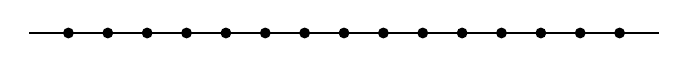
\begin{tikzpicture}[line width=1pt]    
    \draw (-4.0,0) -- (4.0,0); 
    \foreach \x in {-7,...,7}
    \draw [fill] (\x/2,0) circle [radius=0.05];
    \end{tikzpicture}
    \end{center}
    \caption{El dibujo correcto de $\mathbb Z$.}\label{f1.2}
\end{figure}

\begin{figure}[ht]    
    \begin{center}
    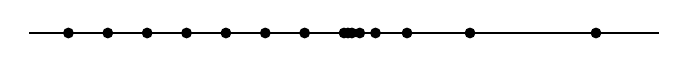
\begin{tikzpicture}[line width=1pt]    
    \draw (-4.0,0) -- (4.0,0); 
    \foreach \x in {-7,...,0}
    \draw [fill] (\x/2,0) circle [radius=0.05];
    \foreach \x in {0.05,0.1,0.2,0.4,0.8,1.6,3.2}
    \draw [fill] (\x,0) circle [radius=0.05];
    \end{tikzpicture}
    \end{center}
    \caption{El dibujo incorrecto de $\mathbb Z$.}\label{f1.3}
\end{figure}

El hecho de que haya espacios vacíos entre los enteros nos lleva a decir que el conjunto $\mathbb Z$ es \textit{discreto} y es esta propiedad la que da origen al nombre ``matemática discreta''. En cálculo y análisis, los procesos de límite son de fundamental importancia, y es preciso usar aquellos sistemas numéricos que son \textit{continuos}, en vez de los discretos.

El siguiente resultado es obvio, pero  debe ser demostrado. Sin embargo,  la demostración es bastante compleja y sólo se da por completitud. 
\begin{proposicion}\label{prop-0-menor-que-1}
$1$ es el menor entero mayor que $0$.
\end{proposicion}
\begin{proof}[Demostración (*)] Primero debemos probar que $0 < 1$. Ahora bien, como $0 \not= 1$ (por axioma \textbf{I4}), por la ley de tricotomía (axioma \textbf{I8}), debe ocurrir que $0 < 1$ o $ 1 < 0$. Supongamos que $1 < 0$, luego por proposición \ref{prop-compatibilidad-negativa}, $1 \cdot 1 > 1 \cdot 0$. Como $1$  es elemento neutro de la multiplicación, obtenemos $1 > 0$, que contradice nuestra suposición. Esta contradicción vino de suponer que $1 < 0$. Por lo tanto, $0 < 1$.

Probaremos ahora que no existe $a$ entero tal que $ 0<a<1$ y lo haremos por el absurdo: supongamos que existe $a \in \mathbb Z$ tal que $0<a<1$ y sea 
$$
X=\{a\in\mathbb Z: 0<a<1\}.
$$
La  suposición que hicimos implica que $X$ es no vacío.  Dado que todos los elementos de $X$ son positivos, $X$ es un subconjunto de $\mathbb Z$ acotado inferiormente ($0$ es cota inferior). Por el axioma del buen orden (\textbf{I12}) resulta que $X$ tiene un elemento mínimo, que llamaremos $a_0$, y cumple
$$
0<a_0<1. 
$$
Usamos ahora la compatibilidad del  producto con  la relación de orden (\textbf{I11}):  por un lado multiplicamos por $a_0$ la desigualdad $0<a_0$ y obtenemos $0<a_0^2$,  y por otro lado multiplicamos por $a_0$ la desigualdad $a_0<1$ y obtenemos $a_0^2<a_0$. Es decir
$$
 0<a_0^2<a_0<1.
$$
La desigualdad $0<a_0^2<1$ dice que $a_0^2\in X$ pero la desigualdad $a_0^2<a_0$ dice que  $a_0$ no es el mínimo elemento de $X$, lo cual es una contradicción pues dijimos que $a_0$ es el mínimo elemento de $X$.  El  absurdo  vino de suponer que existe $a \in \mathbb Z$ tal que   $0<a<1$.
\end{proof}


\subsection*{$\S$ Ejercicios}
\begin{enumerate}
    \item Demostrar que $\ge$ es una relación de orden.
        
    \item Demostrar que dados cualesquiera $a,b,c \in \mathbb Z$ vale que si $a< b$ y $0\le c$, entonces $ac \le bc$. 
        
    \item Demostrar que si $a\le b$ y $c\le 0$, entonces $bc \le ac$.
        
    \item Demostrar que $0\le x^2$ para todo $x$ en $\mathbb Z$.
        
    \item Deducir de la proposición \ref{prop-0-menor-que-1} que $n+1$ es el menor entero mayor que $n$ para todo $n$ en $\mathbb Z$.

    \item Demostrar que si un conjunto $X$ tiene mínimo, este es único. Dicho más formalmente: demostrar que si existen $c,c' \in X$ tal que  $c\le x$ y $c'\le x$ para todo $x \in X$, entonces $c=c'$. 

    \item En cada uno de los siguientes casos decir si el conjunto $X$ tiene o no una cota inferior, y si la tiene, encontrar el mínimo.
    \begin{enumerate}
        \item $X = \{x \in \mathbb Z | x^2\le 16\}.$
        \item $X =\{x \in \mathbb Z | x=2y \text{\ para algún } y \in \mathbb Z\}.$
        \item $X =\{x \in \mathbb Z | x\le 100\,x\} .$
    \end{enumerate}
    \item Un subconjunto $Y$ de $Z$ se dice que tiene una {\em cota superior}\index{cota superior} $c$ si $c\ge y$ para todo $y \in Y$.  Una cota superior que además es un elemento de $Y$ es llamada el {\em máximo} de $Y$. Usar el axioma (\textbf{I12}) para demostrar que si $Y$ es no vacío y tiene una cota superior, entonces tiene máximo. [Ayuda: aplicar el axioma al conjunto cuyos elementos son $-y$ ($y \in Y$).]

    \item Los enteros $n$ que satisfacen $1 \le n \le 25$ están acomodados en forma arbitraria en un arreglo cuadrado de cinco filas y cinco columnas. Se selecciona el máximo  de cada fila, y se denota $s$ al mínimo entre ellos. De manera similar, el mínimo de cada columna es seleccionado y $t$ denota al máximo entre ellos. Demostrar que $s\ge t$ y de un ejemplo en el cual $s\not=t$.
\end{enumerate}
%\end{subsection}

\end{section}

\begin{section}{Definiciones recursivas}\label{1.3}

Sea $\mathbb N$ el conjuntos de enteros positivos, esto es
$$
\mathbb N = \{ n \in \mathbb Z | n\ge 1\},
$$
y denotemos $\mathbb N_0$ el conjunto $\mathbb N \cup \{0\}$, esto
es
$$
\mathbb N_0 = \{ n \in \mathbb Z | n\ge 0\}.
$$
$\mathbb{N}$  es llamado el conjunto de  \textit{números naturales}. Si $X$ es un subconjunto de $\mathbb N$ (o de $\mathbb N_0$)  entonces automáticamente tiene una cota inferior, pues cada elemento $x$ de $X$ satisface $x\ge 1$ (o $x\ge 0$). As{í}, en este caso el axioma del buen orden toma la forma
$$
\begin{aligned}
&\textit{si $X$ es un subconjunto no vacío de $\mathbb N$ o $\mathbb N_0$ entonces $X$
 tiene un mínimo.}
\end{aligned}
$$
Esta la forma más usada en la práctica.

Nuestro primer uso del axioma del buen orden será para justificar un procedimiento muy usual. Frecuentemente encontramos una expresión de la forma $u_n$, donde $n$ indica cualquier entero positivo: por ejemplo, podríamos tener $u_n=3n+2$, o $u_n = (n+1)(n+2)(n+3)$. En estos ejemplos $u_n$ es dado por una fórmula explícita y no existe dificultad en explicar como calcular $u_n$ cuando se nos da un valor específico para $n$. Sin embargo en muchos casos no conocemos una fórmula para $u_n$; es más, nuestro problema puede ser encontrarla. En estos casos pueden darnos ciertos valores de $u_n$ para enteros positivos $n$ peque\~nos, y una relación entre el $u_n$ general y algunos de los $u_r$ con $r<n$. Por ejemplo, supongamos nos es dado 
$$ 
u_1=1, \qquad u_2=2, \qquad u_n =u_{n-1} +u_{n-2}, \qquad n\ge 3.
$$
Para calcular los valores de $u_n$ para todo $n$ de $\mathbb N$ podemos proceder como sigue:
$$
\begin{matrix}
u_3 & = & u_2 + u_1 & = & 2+1 &=& 3, \\
u_4 & = & u_3 + u_2 & = & 3+2 &=& 5, \\
u_5 & = & u_4 + u_3 & = & 5+3 &=& 8,
\end{matrix}
$$
y así siguiendo.  Éste es un ejemplo de una \textit{definición recursiva}. Es ``obvio'' que el método dará un valor único de $u_n$ para todo entero positivo $n$. Pero hablando estrictamente necesitamos el axioma del buen orden para justificar la conclusión a través de las siguientes líneas.

Supongamos que existe un entero positivo $n$ para el cual $u_n$ no está definido de manera única. Entonces por el axioma del buen orden existe un entero positivo mínimo $m$ con esta propiedad. Como $u_1$ y $u_2$ están explícitamente definidos, $m$ no es $1$ o $2$ y la ecuación $u_m =u_{m-1} +u_{m-2}$ es aplicable. Por la definición de $m$, $u_{m-1}$ y $u_{m-2}$ están definidos de manera única, y la ecuación nos da un valor único para $u_m$ , contrariamente a la hipótesis. La contradicción surge de suponer que no está bien definido para algún $n$, y por lo tanto esta suposición debe ser falsa.

El lector no debe desanimarse por el uso de argumentos tan retorcidos para establecer algo que es ``obviamente'' verdadero. En primer lugar, no debemos usar resultados ilegítimamente (sin demostrarlos), y en segundo lugar, el hecho de que el resultado sea ``obvio'' simplemente indica que estamos trabajando con la correcta representación mental de $\mathbb N$ y $\mathbb Z$. Una vez que hemos establecido esa representación sobre bases firmes podemos empezar a extendernos y obtener resultados que no sean tan ``obvios''.

El método de definición recursiva aparecerá bastante seguido en el resto del apunte. Existen otras formas de este procedimiento que se ``esconden'' por su notación. ¿Qué significan las siguientes expresiones?
$$
\sum_{r=1}^{n} 2r-1,\qquad 1+3+5+\cdots +(2n-1).
$$
Claramente no basta decir que uno significa lo mismo que el otro, porque cada uno contiene un misterioso símbolo, $\sum$ y $\cdots$, respectivamente. Lo que deberíamos decir es que cada uno de ellos es equivalente a la expresión $s_n$, dada por la siguiente definición recursiva:
$$
s_1= 1, \qquad s_n = s_{n-1} +(2n-1), \qquad n\ge 2.
$$

Esto hace ver claro que ambos símbolos misteriosos son, en realidad, una forma de acortar una definición recursiva, y que por lo tanto son expresiones definidas para todo $n$ en $\mathbb N$.

Ideas similares pueden aplicarse a la definición de productos tal como $n!$ (que se lee $n$ \textit{factorial}). Si decimos que
$$
n!=1 \cdot 2 \cdot 3 \cdots n,
$$
el significado es bastante claro para cualquiera. Pero para precisar (y hacerlo claro para una computadora) debemos usar las definiciones recursivas.

\begin{definicion} Sea $n \in \N$ sean $a_i$  $1 \le i \le n$ una secuencia de números (enteros, reales, etc.). Entonces $\sum_{i=1}^{n} a_i$  denota la función recursiva definida  
    $$
    \sum_{i=1}^{1} a_i= a_1, \qquad \sum_{i=1}^{n} a_i = \sum_{i=1}^{n-1} a_i+ a_{n} \quad (n\ge 2).
    $$
    En  este caso  decimos que  $\sum_{i=1}^{n} a_i$ es la \textit{sumatoria} de los $a_i$ de $i=1$  a $n$. El símbolo $\prod_{i=1}^{n} a_i$ denota la función recursiva definida  
    $$
    \prod_{i=1}^{1} a_i= a_1, \qquad \prod_{i=1}^{n} a_i = \prod_{i=1}^{n-1} a_i \cdot  a_{n} \quad (n\ge 2).
    $$
    En  este caso  decimos que  $\prod_{i=1}^{n} a_i$ es la \textit{productoria} de los $a_i$ de $i=1$  a $n$. 
\end{definicion}



En  el caso de $n!$ se puede  o bien definir como $\prod_{i=1}^{n} i$, o bien como
$$
1!=1,\qquad n!=n \cdot (n-1)! \quad (n\ge 2).
$$

Otro caso que debemos mencionar es  el de la definición de ``$n$-ésima potencia'': sea $x$ un  número, si $n \in \N$ definimos
$$
x^1=x,\qquad x^n= x \cdot x^{n-1} \quad (n\ge 2).
$$
Por completitud,  definimos $x^0=1$. 

\subsection*{$\S$ Ejercicios}
\begin{enumerate}
    \item En el caso siguiente calcule (donde sea posible) los valores de $u_1$, $u_2$, $u_3$ y $u_4$ dados por las ecuaciones. Si no puede calcular los valores explicar porque la definición no esta bien.
    \begin{enumerate}
        \item $u_1 = 1$,\qquad $u_2=1$,\qquad $u_n = u_{n-1} +2 u_{n-2}$,\qquad $n \ge 3$. 
        \item $u_1 = 1$,\qquad $u_n = u_{n-1} +2u_{n-2}$,\qquad $n \ge 2$. 
        \item $u_1 = 0$,\qquad $u_n = nu_{n-1}$,\qquad $n \ge 2$.
    \end{enumerate}

    \item Sea $u_n$ definido por las ecuaciones
    $$
    u_1=2,\qquad u_n= 2^{u_{n-1}}, \qquad n\ge 2.
    $$
    ¿Cuál es el primer valor de $n$ para el cual no se puede calcular $u_n$ usando una calculadora de bolsillo o de su celular?

    \item Escribir fórmulas explícitas para las expresiones $u_n$ definidas por las siguientes ecuaciones.
    \begin{enumerate}
        \item $u_1 = 1$,\qquad $u_n = u_{n-1} +3$,\qquad $n \ge 2$. 
        \item $u_1 = 1$,\qquad $u_n = n^2u_{n-1}$,\qquad $n \ge 2$.
    \end{enumerate}
\end{enumerate}
\end{section}


\begin{section}{El principio de inducción}\label{1.4}

Supongamos que nos piden que demostremos el resultado
$$
1+3+5+\cdots+(2n-1) = n^2.
$$
En otras palabras, debemos demostrar que la expresión de la izquierda definida recursivamente es igual a la expresión definida explícitamente por la fórmula de la derecha, para todos los enteros positivos $n$. Podemos proceder como sigue.

La fórmula es ciertamente correcta cuando $n=1$ puesto que $1=1^2$.  Supongamos que es correcta para un valor específico de $n$, digamos para $n=k$, de modo que
$$
1+3+5+\cdots+(2k-1) = k^2.
$$
Podemos usar esto para simplificar la expresión definida recursivamente a la izquierda cuando $n$ es igual a $k+1$,
$$
\begin{aligned}
1+3+5+\cdots+(2k+1) &= 1+3+5+\cdots+(2k-1) +(2k+1) \\
&=k^2 +(2k+1) \\
&=(k+1)^2.
\end{aligned}
$$
Por lo tanto si el resultado es correcto cuando $n=k$, entonces lo es cuando $n=k+1$. Se comienza observando que si es correcto cuando $n=1$, debe ser por lo tanto correcto cuando $n=2$. Con el mismo argumento como es correcto cuando $n=2$ debe serlo cuando $n=3$. Continuando de esta forma veremos que es correcto para todos los enteros positivos $n$.

La esencia de este argumento es comúnmente llamada \textit{principio de inducción}. Es una técnica poderosa, fácil de aplicar y la aplicaremos frecuentemente. Pero primero debemos examinar sus bases lógicas y para hacerlo necesitamos una formulación más general. Con $S$ denotemos al subconjunto de $\mathbb N$ para el cual el resultado es correcto: por supuesto, nuestra intención es probar que $S$ es todo $\mathbb N$. El primer paso es probar que $1$ pertenece a $S$, y luego demostraremos que si $k$ pertenece a $S$, también $k+1$. Entonces lo pensamos paso a paso, un procedimiento infinito, y concluimos que $S=\mathbb N$. Afortunadamente el pensarlo paso a paso no es esencial debido a que el principio de inducción es consecuencia de los axiomas que elegimos tan cuidadosamente para $\mathbb Z$ y $\mathbb N$. Más específicamente es consecuencia del axioma del buen orden.

\begin{teorema}[Principio de inducción]\label{t1.4} Supongamos que $S$ es un subconjunto de $\mathbb N$ que satisface las condiciones \index{principio de inducción}
\begin{enumerate}
\item $1 \in S$,
\item para cada $k \in \mathbb N$, si $ k \in S$ entonces $k+1\in S$.
\end{enumerate}
Entonces se sigue que $S=\mathbb N$.
\end{teorema}
\begin{proof}Si la conclusión es falsa, $S \not= \mathbb N$ y
el conjunto complementario $S^{\text{c}}$ definido por
$$
S^{\text{c}}= \{ r \in \mathbb N | r\not\in S\}
$$
 es no vacío. Por el axioma del buen orden, $S^{\text{c}}$ tiene un menor elemento $m$. Como $1$ pertenece a $S$, $m\not=1$. Se sigue que $m-1$ pertenece a $\mathbb N$ y como $m$ es el mínimo de $S^{\text{c}}$, $m-1$ debe pertenecer a $S$. Poniendo $k=m-1$ en la condición (b), concluimos que $m$ esta en $S$, lo cual contradice el hecho de que $m$ pertenece a $S^{\text{c}}$. De este modo, la suposición $S \not= \mathbb N$ nos lleva a un absurdo, y por lo tanto tenemos $S= \mathbb N$. 
 \end{proof}

En la práctica, generalmente presentamos una ``demostración por inducción'' en términos más descriptivos. El hecho de que el resultado es verdadero cuando $n=1$ se llama \textit{base de la inducción} o \textit{caso base}, (b) es llamado  el {\em paso inductivo} y la suposición de que es verdadero cuando $n=k$ es llamada \textit{hipótesis inductiva}\index{hipótesis inductiva}. Cuando se utilizan estos términos, no es necesario introducir explícitamente el conjunto $S$.


El principio de inducción es útil para probar la veracidad de propiedades relativas a los números naturales. Por ejemplo, consideremos las siguientes propiedades $P(n)$, $Q(n)$ y $R(n)$:
\begin{enumerate}[label=\textit{\alph*)}]
\item $P(n)$ es la propiedad: $2n -1 < n^2 + 1$,
\item $Q(n)$ es la afirmación: si $n$ es par entonces $n$ es divisible por 4,
\item $R(n)$ es la afirmación: $2n < n- 1$.
\end{enumerate}
Intuitivamente notamos que $P(n)$ es verdadera para cualquier $n$ natural, $Q(n)$ lo es para algunos valores de $n$ y es falsa para otros y $R(n)$ es falsa para todo valor de $n$. Sin embargo, para verificar realmente que la propiedad $P(n)$ es verdadera para todo $n$ natural no podemos hacerlo probando para cada $n$ en particular. Resulta entonces muy útil la siguiente versión equivalente del principio de inducción.

\begin{teorema}\label{induccion2} Sea $P(n)$ una propiedad para $n \in \mathbb N$ tal que:
\begin{enumerate}[label=\textit{\alph*)}]
\item\label{it.ind1} $P(1)$ es verdadera.
\item\label{it.ind2} Para todo $k \in \mathbb N$, $P(k)$ verdadera implica $P(k + 1)$ verdadera.
\end{enumerate}
Entonces $P(n)$ es verdadera para todo $n \in \mathbb N$.
\end{teorema}
\begin{proof} Basta tomar
$$S = \{n \in \mathbb N| P(n) \text{ es verdadera} \}.$$
Entonces $S$ es un subconjunto de $\mathbb N$ y las condiciones \ref{it.ind1} y \ref{it.ind2} nos dicen que $1 \in S$ y  si $ k \in S$ entonces $k+1\in S$. Por el teorema \ref{t1.4} se sigue que $S= \mathbb N$, es decir que $P(n)$ es verdadera para todo $n$.
natural.
\end{proof}


En la notación del teorema anterior, \ref{it.ind1} es llamado  el {\em caso base}, \ref{it.ind2} es llamado el  {\em paso inductivo} y $P(k)$ es llamada la {\em hipótesis inductiva}. El paso inductivo  consiste en probar que $P(k) \Rightarrow P(k + 1)$ o, equivalentemente, podemos suponer $P(k)$ verdadera y a partir de ella probar $P(k + 1)$. 


\begin{ejemplo}\label{ejemplo141} Sea $a\in \mathbb Z$ tal que $0<a$. Probemos que $0<a^n$ para todo $n \in \mathbb N$.
\end{ejemplo}
\begin{proof}
\

\noindent (\textit{Caso  base}) El resultado es verdadero
cuando $n=1$ pues $ 0 < a=a^1$.

\noindent (\textit{Paso  inductivo})
 Supongamos que el resultado verdadero cuando $n=k$, o sea, que la hipótesis inductiva es $0 < a^k$. Entonces, como $0<a$, multiplicando por $a$ ambos lados de la desigualdad obtenemos, por la compatibilidad de $<$ con el producto, que $a\cdot 0 < a^k \cdot a$, es decir $0<a^{k+1}$.  Luego el resultado es verdadero cuando $n=k+1$ y por el principio de inducción, es verdadero para todos los enteros positivos $n$.
\end{proof}

\begin{ejemplo*} El entero $x_n$ esta definido recursivamente por
$$
x_1=2, \qquad x_n=x_{n-1} +2n, \qquad n\ge 2.
$$
Demostremos que
$$
x_n = n(n+1) \qquad \text{ para todo } n\in \mathbb N.
$$
\end{ejemplo*}
\begin{proof}
\    

\noindent(\textit{Caso  base}) El resultado es verdadero cuando $n=1$ pues $ 2 = 1 \cdot 2$.

\noindent (\textit{Paso  inductivo})
 Supongamos que el resultado verdadero cuando $n=k$, o sea, que la hipótesis inductiva es $x_k = k(k+1)$. Entonces
$$
\begin{matrix} 
x_{k+1} &= x_k + 2(k+1) \hfill &\qquad &\text{por la definición recursiva} \hfill \\
&= k(k+1)+2(k+1) \hfill &\qquad &\text{por hipótesis inductiva}\hfill \\
&= (k+1)(k+2). \hfill &
\end{matrix}
$$
Luego el resultado es verdadero cuando $n=k+1$ y por el principio de inducción, es verdadero para todos los enteros positivos $n$.
\end{proof}


Existen varias formas modificadas del principio de inducción. A veces es conveniente tomar como base inductiva el valor $n=0$, por otro lado puede ser apropiado tomar un valor como $2$ o $3$ porque los primeros casos pueden ser excepcionales. Cada problema debe ser tratado según sus características. Otra modificación útil es tomar como hipótesis inductiva la suposición de que el resultado es verdadero para todos los valores $n\le k$, más que para $n=k$ solamente. Esta formulación es llamada a veces el principio de inducción \textit{completa}. Todas esas modificaciones pueden justificarse con cambios triviales en la demostración del teorema \ref{t1.4}

El siguiente teorema incorpora todas las modificaciones del principio de inducción mencionadas más arriba.

\begin{teorema}[Principio de inducción completa] Supongamos que $n_0$ es cualquier entero (no necesariamente positivo), y sea $X$ el conjunto de enteros $n$ tal que $ n \ge n_0$. Sea $S$ un subconjunto de $X$ que satisface las condiciones: \index{principio de inducción completa}
\begin{enumerate}[label=\textit{\alph*)}]
\item\label{it.indcompleta_1} $n_0 \in S$,
\item\label{it.indcompleta_n} si $h\in S$ para todo $h$ en el rango $n_0 \le h \le k$ entonces $k+1 \in S$.
\end{enumerate}
Entonces se sigue que $S=X$.
\end{teorema}
\begin{proof}[Demostración (*)]
Si la conclusión es falsa, $S \not= X$ y el conjunto complementario (en $X$)  $S^{\text{c}}$ definido por
$$
S^{\text{c}}= \{ r \in X | r\not\in S\}
$$
es no vacío. Como $X$ es un conjunto acotado inferiormente por $n_0$, por el axioma del buen orden, $S^{\text{c}}$ tiene un menor elemento $m$. Como $n_0$ pertenece a $S$, $m\not=n_0$. Se sigue que $m-1$ pertenece a $X$ y como $m$ es el mínimo de $S^{\text{c}}$, $m-1$ debe pertenecer a $S$. Poniendo $k=m-1$ en la condición \ref{it.indcompleta_n}, concluimos que $m$ esta en $S$, lo cual contradice el hecho de que $m$ pertenece a $S^{\text{c}}$. De este modo, la suposición $S \not= X$ nos lleva a un absurdo, y por lo tanto tenemos $S= X$.
\end{proof}

Como se podrá observar, la demostración es muy similar a  la del teorema \ref{t1.4}. El teorema anterior lo podemos utilizar para la demostración de propiedades dependientes de números enteros.

\begin{teorema}\label{ind-completa} Sea $n_0$ número entero y sea $P(n)$ una propiedad para $n \ge n_0$ tal que:
\begin{enumerate}[label=\textit{\alph*)}]
\item $P(n_0)$ es verdadera.
\item Si $P(h)$ verdadera para toda $h$ tal que $n_0 \le h \le k$ implica $P(k + 1)$ verdadera.
\end{enumerate}
Entonces $P(n)$ es verdadera para todo $n \ge n_0$.
\end{teorema}
\begin{proof} Ejercicio.
\end{proof}



\begin{ejemplo*}
Sean $$u_1 = 3,\qquad u_2 = 5,\qquad u_n = 3u_{n-1}- 2u_{n-2},\qquad  n \ge 3.$$
Probemos que $u_n = 2^n + 1$, para todo $n \in  \mathbb N$.
\begin{proof}[Solución] Aquí usaremos una extensión natural del principio de inducción: en este caso, el caso base es $n=1$ y $n=2$.

\noindent(\textit{Caso  base}) El resultado es verdadero cuando $n= 1$ pues $3 = 2^1+1$ y para $n=2$ pues $ 5 =2^2+1$.

\noindent (\textit{Paso  inductivo}) Supongamos que $k \ge 2$ y el resultado  es cierto para los $h$ tales que  $1 \le h \le k$. Es decir que $u_h = 2^h+1$ para $1 \le h \le k$ y $k \ge 2$ (hipótesis inductiva), entonces
$$
\begin{matrix} u_{k+1} &= 3u_k -2u_{k-1} \hfill &\qquad &\text{por definición recursiva} \hfill \\
&= 3(2^k+1)-2(2^{k-1}+1) \hfill &\qquad &\text{por hipótesis inductiva}\hfill \\
&= 3\cdot 2^k+3-2\cdot 2^{k-1}-2 \hfill &\qquad & \\
&= 3\cdot 2^k+1- 2^{k} \hfill &\qquad & \\
&= 2\cdot 2^k+1 \hfill &\qquad & \\
&= 2^{k+1}+1. \hfill &\qquad & 
\end{matrix}
$$
\end{proof}
\end{ejemplo*}


\begin{ejemplo*}
Sea $a \in \mathbb Z$ y $n \in \mathbb N$. Definimos $a^n$ de la siguiente manera:
\begin{equation}\label{potencia}
a^1 = a, \qquad a^{n+1} = a^{n}\cdot a \qquad \text{ para $n >1$.}
\end{equation}
Si $n,m \in \mathbb N$ verifiquemos las siguientes propiedades

\begin{enumerate}[label=\textit{\alph*)}]
\item \label{pot+pot} $a^{n} \cdot a^m = a^{n+m}$.
\item \label{potpot} $(a^n)^m = a^{nm}$
\end{enumerate}
\end{ejemplo*}
\begin{proof}[Solución] 
    Veamos la afirmación \ref{pot+pot}. Se fijará $n$ y se hará inducción sobre $m$. 
    
    \noindent(\textit{Caso  base}) Debemos ver que $a^{n} \cdot a^1 = a^{n+1}$, lo cual es verdadero por la definición recursiva (\ref{potencia}). 
    
    \noindent (\textit{Paso  inductivo}) Supongamos que el resultado es verdadero para $m=k$, es decir que $a^{n} \cdot a^k = a^{n+k}$ (hipótesis inductiva). Veamos que  $a^{n} \cdot a^{k+1} = a^{n+k+1}$. Ahora bien, 
    \begin{alignat*}2
        a^{n} \cdot a^{k+1} &= a^{n} \cdot a^{k} \cdot a &\qquad  &\text{definición (\ref{potencia})} \\
        &= a^{n+k} \cdot a &\qquad &\text{hipótesis inductiva} \\
        &= a^{n+k+1} &\qquad  &\text{definición (\ref{potencia})}. 
    \end{alignat*}
    
    Probemos ahora \ref{potpot}. Al igual que antes, Se fijará $n$ y se hará inducción sobre $m$.
    
    \noindent(\textit{Caso  base}) Debemos ver que $(a^n)^1 = a^n$, lo cual es verdadero por la definición recursiva (\ref{potencia}). 
    
    
    \noindent (\textit{Paso  inductivo}) Supongamos que el resultado es verdadero para $m=k$, es decir que  $(a^n)^k = a^{nk}$ (hipótesis inductiva). Veamos que  $(a^n)^{k+1} = a^{n(k+1)}$. 
    \begin{alignat*}2
        (a^n)^{k+1} &= (a^n)^{k} \cdot a^n &\qquad  &\text{definición (\ref{potencia})} \\
        &= a^{nk} \cdot a^n &\qquad &\text{hipótesis inductiva} \\
        &= a^{nk+n} &\qquad  &\text{por \ref{pot+pot}}\\
        &= a^{n(k+1)}. &\qquad  &
    \end{alignat*}
\end{proof}

\subsection*{$\S$ Ejercicios}
\begin{enumerate}
\item Usar el principio de inducción para demostrar que
$$
1^2+2^2+\cdots +n^2 = \frac16 n(n+1)(2n +1)
$$
para todos los enteros positivos $n$.

\item Hacer una tabla de valores de
$$
S_n = 1^3+2^3+\cdots +n^3
$$
para $1 \le n\le 6$. Basándose en su tabla sugiera una fórmula para $S_n$. [Ayuda: los valores de $S_n$ son cuadrados perfectos.] Usar el principio de inducción para establecer que la fórmula es correcta para todo $n\ge 1$. (Si el método falla !`su fórmula es equivocada!)

\item Probar que
$$
1^4+2^4+\cdots+n^4= \frac{1}{30}n(n+1)(2n+1)(3n^2+3n+1).
$$
\item Usar el principio de inducción para probar que $2^n>n+1$ para todo entero $n\ge2$.

\item Encontrar el menor entero positivo $n_0$ para el cual sea verdadero que $n! \ge 2^n$. Tomando el caso $n=n_0$ como la base inductiva, demostrar que el resultado vale para $n\ge n_0$.

\item En los siguientes casos encontrar los valores apropiados de $n_0$ para la base inductiva y demostrar que la afirmación es verdadera
para todos los $n\ge n_0$.
\begin{enumerate}
    \item $n^2 +6n + 9 \ge 0,$
    \item $n^3 \ge 6n^2.$
\end{enumerate}

\end{enumerate}
\end{section}

\begin{section}{Ejercicios}
    \begin{enumerate}
        \item\label{prob1} Demostrar las siguientes afirmaciones donde $a$, $b$, $c$ y $d$ son siempre números enteros. Justificar cada uno de los pasos en cada demostración indicando el axioma o resultado que utiliza.
        \begin{enumerate}
            \item  $a=-(-a)$
            \item  $a=b\,$ si y sólo si $\,-a=-b$
            \item  $a+a=a$ implica que  $a=0$.
        \end{enumerate}

        \item Idem \ref{prob1}.
        \begin{enumerate}
            \item $0<a\,$ y $\,0<b\,$ implican $\,0<a\cdot b$
            \item $a<b\,$ y $\,c<0$ implican $\,b\cdot c<a\cdot c$
        \end{enumerate}

        \item  Probar las siguientes afirmaciones, justificando los pasos que realiza.
        \begin{enumerate}
            \item Si $0 < a$  y $\,0<b\,$ entonces $\,a<b\,$ si y sólo si $a^2<b^2$.
            \item Si $a\neq 0$  entonces $a^2>0$.
            \item Si $a\neq b$  entonces $a^2+b^2>0$.
            \item Probar que si $a+c <b+c$ entonces $a<b$.
        \end{enumerate}

        \item Calcular evaluando las siguientes expresiones:
        \begin{multicols}{4}
        \begin{enumerate}
            \item \quad $\displaystyle{\sum_{r=0}^4 r}$
            \item \quad $\displaystyle{\prod_{i=1}^5 i}$
            \item  \quad $\displaystyle{\sum_{k=-3}^{-1} \frac{1}{k(k+4)}}$
            \item \quad $\displaystyle{\prod_{n=2}^7 \frac{n}{n-1}}$
        \end{enumerate}
        \end{multicols}

        \item Calcular:
        \begin{multicols}{2}
        \begin{enumerate}
            \item \quad $2^{10} - 2^{9}$
            \item \quad $3^2 2^5 - 3^5 2^2$
            \item \quad $(2^2)^n - (2^n)^2$
            \item \quad $(2^{2^n} + 1)  (2^{2^n} - 1)$
        \end{enumerate}
        \end{multicols}

        \item Dado un natural $m$, probar que $\forall n \in {\mathbb N} $; $x$, $y \in {\mathbb R}$, se cumple:
        \begin{multicols}{3}
        \begin{enumerate}
            \item $x^n \cdot x^m = x^{n+m}$
            \item $(x\cdot y)^n=x^n\cdot y^n$
            \item $(x^n)^m = x^{n\cdot m}$
        \end{enumerate}
        \end{multicols}

        \item Analizar la validez de las siguientes afirmaciones:
        \begin{enumerate}
            \item  $(2^{2^n})^{2^k} = 2^{2^{n+k}}$,  $n$, $k \in {\mathbb N}$.
            \item $(2^n)^2 = 4^n$, $n \in {\mathbb N}$.
            \item $2^{7+11} = 2^7 + 2^{11}$.
        \end{enumerate}

        \item Probar que $\sum_{i=0}^n 2^i = 2^{n+1} -1$ ($n \ge 0$). 

        \item Probar las siguientes afirmaciones usando inducción en $n$:
        \begin{enumerate}
            \item $n^2\leq 2^n$ para todo $n\in{\mathbb N}$, $n>3$ .
            \item $\forall n \in {\mathbb N}$,\ $3^n \ge 1 + 2^n$.
        \end{enumerate}

        \item Demostrar por inducción  las siguientes igualdades:
        \begin{enumerate}
            \item  $\displaystyle{ \sum_{k=1}^n (a_k + b_k) = \sum_{k=1}^n a_k + \sum_{k=1}^n b_k}$, $n\in \mathbb N$.
            \item  $\displaystyle{ \sum_{j=1}^n j = \frac{n(n+1)}{2}}$, $n\in \mathbb N$, $n\in \mathbb N$.
            \item  $\displaystyle{ \sum_{i=1}^n i^2 = \frac{n(n+1)(2n+1)}{6}}$, $n\in \mathbb N$.
            \item  $\displaystyle{ \sum_{k=0}^n (2k+1) = (n+1)^2}$, $n\in \mathbb N_0$.
            \item  $\displaystyle{ \sum_{i=1}^n i^3 = \left( \frac{n(n+1)}{2 }\right)^2}$, $n\in \mathbb N$.
            \item  $\displaystyle{ \sum_{k=0}^n a^k = \frac{a^{n+1}-1}{a-1}}$, donde $a\in {\mathbb R}$, $a \neq 0,\ 1$, $n\in \mathbb N_0$.
            \item  $\displaystyle{ \prod_{i=1}^n \frac{i+1}{i} = n+1}$, $n\in \mathbb N$.
            \item $\displaystyle{ \sum_{i=1}^n \frac{1}{4i^2-1} = \frac{n}{2n+1}}$, $n\in \mathbb N$.
            \item $\displaystyle{ \sum_{i=1}^n i^2\, /\, \sum_{j=1}^n j = \frac{2n+1}{3}}$, $n\in \mathbb N$.
            \item $\displaystyle{ \prod_{i=2}^n \left(1-\frac{1}{i^2}\right) = \frac{n+1}{2n}}$, $n\in \mathbb N$ y $ n\ge 2$.
            \item Si $a\in \mathbb R$ y $a\geq -1$, entonces $(1+a)^n\geq 1+n\cdot a$, $\forall \, n \in \mathbb N$.
            \item Si $a_1,\dots,a_n \in \mathbb R$, entonces $\displaystyle{\sum_{k=1}^n a_{k}^{2}\leq \left(\sum_{k=1}^n |a_{k}|\right)^{2}}$, $n\in \mathbb N$.
            \item Si $a_1,\dots,a_n \in \mathbb R$ y $0<a_i<1 \forall \, i$, entonces $(1-a_1)\cdots(1-a_n)\ge 1-a_1-\cdots -a_n$, $n\in \mathbb N$.
        \end{enumerate}

        \item Hallar $n_0 \in {\mathbb N}$ tal que $\forall n \ge n_0$ se cumpla que $n^2 \ge 11 \cdot n + 3$.

        \item Sea $u_1=3$, $u_2=5$ y $u_n=3 u_{n-1} - 2 u_{n-2}$ con $n\in \mathbb N$, $n\geq 3$.
        Probar que $u_n=2^n+1$.

        \item Sea $\{ u_n \}_{n \in \mathbb N}$ la sucesión definida por recurrencia como sigue: $u_1 = 9$, $u_2 = 33$, $u_n = 7u_{n-1} - 10u_{n-2}$, $\forall n \geq 3$. Probar que $u_n = 2^{n+1} + 5^n$, para todo $n \in \mathbb N$.

        \item Sea $u_n$ definida recursivamente por: 
        $$u_1=2,\;\; u_n=2+\sum_{i=1}^{n-1}2^{n-2i}u_i \;\;\forall\; n >1.$$
        \begin{enumerate}
            \item Calcule $u_2$ y $u_3$.
            \item Proponga una fórmula para el término general $u_n$ y pruébela por inducción.
        \end{enumerate}

        \item Las siguientes proposiciones no son válidas para todo $n \in {\mathbb N}$. Indicar en qué paso del principio de inducción falla la demostración:
        \begin{multicols}{3}
        \begin{enumerate}
            \item  $n=n^2$,
            \item  $n=n+1$,
            \item  $3^n = 3^{n+2}$,
            \item  $3^{3n} = 3^{n+2}$.
        \end{enumerate}
        \end{multicols}

        \item Encuentre el error en los siguientes argumentos de inducción.
        \begin{enumerate}
            \item  Demostraremos que $5n+3$ es múltiplo de 5 para todo $n\in \mathbb N$.

            Supongamos que $5k+3$ es múltiplo de 5, siendo $k\in \mathbb N$. Entonces existe
            $p\in \mathbb N$ tal que  $5k+3=5p$. Probemos que $5(k+1)+3$ es múltiplo de 5:
            Como
            $$
            5(k+1)+3=(5k+5)+3=(5k+3)+5=5p+5=5(p+1),
            $$
            entonces obtenemos que $5(k+1)+3$ es múltiplo de 5. Por lo tanto, por el principio
            de inducción, demostramos que $5n+3$ es múltiplo de 5 para todo $n\in \mathbb
            N$.
            \item Sea $a\in\mathbb R$, con $a\neq 0$. Vamos a demostrar que para todo entero no negativo $n$, $a^n=1$.

            Como $a^0=1$ por definición, la proposición es verdadera para $n=0$. Supongamos
            que para  un entero $k$, $a^m=1$ para $0\leq m \leq k$. Entonces
            $a^{k+1}= \frac{a^k a^k}{a^{k-1}}=\frac{1\cdot1}1=1$.
            Por lo tanto, el principio de inducción fuerte implica que $a^n=1$ para todo $n\in \mathbb N$.
        \end{enumerate}

        \item* La \emph{sucesión de Fibonacci} se define recursivamente de la siguiente manera:
        $$
        u_1=1,\quad u_2=1,\quad u_{n+1}=u_{n}+u_{n-1}, \, n\geq 2.
        $$
        Los primeros términos de esta sucesión son: $1,1,2,3,5,8,13,\ldots$

        Demostrar por inducción que el término general de esta sucesión se puede calcular mediante la fórmula
        \[ u_n= \frac{1}{\sqrt{5}}\left[\left(\frac{1+\sqrt{5}}{2}\right)^n-\left(\frac{1-\sqrt{5}}{2}\right)^n\right].\]
        (\textit{Ayuda:} usar que $\frac{1+\sqrt{5}}{2}$ y $\frac{1-\sqrt{5}}{2}$ son las raíces de la ecuación cuadrática $x^2-x-1=0$ y por lo tanto  $\left(\frac{1\pm\sqrt{5}}{2}\right)^{n+1} = \left(\frac{1\pm\sqrt{5}}{2}\right)^{n}+\left(\frac{1\pm\sqrt{5}}{2}\right)^{n-1}$).
    \end{enumerate}
\end{section}





\chapter[Conteo]{Conteo}\label{cap.conteo}

Intutivamente, diremos que un conjunto $A$ es finito si podemos contar la cantidad de elementos que tiene. En ese caso denotaremos $|A|$ la cantidad de elementos de $A$ y la llamaremos el {\em cardinal de $A$}\index{cardinal de un conjunto}.  

Formalmente, un conjunto $A$ es finito y tiene  cardinal $n$  si existe una función $f: \{1,\ldots,n\} \to A$ biyectiva. Sin embargo,  a lo largo del curso usaremos sólo la definición intuitiva y  no formal de cardinal, más que suficiente para aprender los principios básicos de conteo.  

\begin{section}{Principios básicos}


\subsection*{El principio de adición}

Se puede realizar una acción $X$ de $n$ formas distintas o, alternativamente, se puede realizar otra acción $Y$ de $m$ formas distintas. Entonces el número de formas de realizar la acción ``$X$ o $Y$'' es $n + m$.

\begin{ejemplo}\label{cine} Supongamos que una persona va a salir a pasear  y puede ir al cine donde hay $3$ películas en cartel o al teatro donde hay $4$ obras posibles. Entonces, tendrá un total de $3+4=7$ formas distintas de elegir el paseo. 
\end{ejemplo}


Este principio es el más básico del conteo y más formalmente dice que si $A$ y $B$ son conjuntos finitos disjuntos, entonces 
\begin{equation*}
|A \cup B| =|A|+|B|.
\end{equation*}
El principio es fácilmente generalizable a varios conjuntos.

\begin{proposicion}\label{principiodeadicion}
Sean $A_1,\ldots,A_n$ conjuntos finitos tal que $A_i \cap A_j = \emptyset$ cuando $i\not=j$, entonces 
\begin{equation*}
|A_1 \cup \cdots \cup A_n| =|A_1|+\cdots+|A_n|.
\end{equation*}
\end{proposicion}



\begin{proof} 
La  prueba se hace por inducción en $n$. Debemos probar 
\begin{align*}
P(n) =\; &\text{Si $A_1,\ldots,A_n$ conjuntos finitos disjuntos dos a dos, entonces }\\  &|A_1 \cup \cdots \cup A_n| =|A_1|+\cdots+|A_n|.
\end{align*}

\noindent({\em Caso base $n=1$}) En este caso no hay nada que probar pues  $|A_1|=|A_1|$.

\noindent({\em Paso inductivo}) La hipótesis inductiva es $P(k)$ y debemos probar que $P(k) \Rightarrow P(k+1)$. Si denotamos $B = A_1 \cup \cdots \cup A_k$, entonces 
$$
A_1 \cup \cdots \cup A_{k+1} = B \cup A_{k+1}
$$
Ahora bien, si $x \in B \cap A_{k+1}$, entonces $x \in A_i$ para algún $i < k+1$ y $x \in A_{k+1}$. Como $A_{i} \cap A_{k+1} = \emptyset$, se produce un absurdo  que viene de suponer que existía un elemento en $B \cap A_{k+1}$. Luego   $B \cap A_{k+1}= \emptyset$ y por el principio de adición  $|B \cup A_{k+1}| = |B|+|A_{k+1}|$. 

Por la hipótesis inductiva tenemos que 
$$
|B| = |A_1 \cup \cdots \cup A_k| =|A_1|+\cdots+|A_k|,
$$
Luego
$$
|A_1 \cup \cdots \cup A_k \cup  A_{k+1}| = |B|+|A_{k+1}| = |A_1|+\cdots+|A_k|+|A_{k+1}|.
$$
\end{proof}



Si $A$ y $B$ no son disjuntos, cuando sumamos $|A|$ y $|B|$ estamos contando $A \cap B$ dos veces. Entonces, para
obtener la respuesta correcta debemos restar $|A \cap B|$ y obtenemos
$$
|A \cup B| = |A|+|B| - |A \cap B|.
$$
Generalizar la fórmula de arriba a más conjuntos no es del todo sencillo y es el  llamado principio del tamiz o principio de inclusión-exclusión (ver apéndice \ref{ape.principio_del_tamiz}). 


%\vskip .3cm

\subsection*{El principio de multiplicación}

Suponga que una actividad consiste de $2$ etapas y la primera etapa puede ser realizada de $n_1$ maneras y la etapa $2$  puede realizarse de $n_2$  maneras, independientemente de como se ha hecho la etapa $1$. Entonces toda la actividad puede ser realizada de $n_1\cdot n_2$  formas distintas.


\begin{ejemplo*}
Supongamos que la persona del ejemplo \ref{cine} tiene suficiente tiempo y dinero para ir primero al cine y luego al teatro. Entonces tendrá  $3 \cdot 4=12$ formas distintas de hacer el paseo.
\end{ejemplo*}


Formalmente, si $A,B$ conjuntos y definimos el {\em producto cartesiano}\index{producto cartesiano} entre $A$ y $B$ por
$$
A \times B = \{(a,b): a \in A, b \in B\}.
$$
Entonces si $A$ y $B$ son conjuntos finitos se cumple que
$$
|A \times B| = |A|\cdot|B|.  
$$

\end{section}

\begin{section}{Selecciones ordenadas con repetición}

Un aplicación inmediata del principio de multiplicación  es que nos permite calcular la cantidad de selecciones ordenadas con repetición. 

\begin{ejemplo*} Sea  $X = [[ 1 , 3]] = \{ 1, 2, 3 \}$ ¿de cuántas formas se pueden elegir dos de estos números en forma ordenada?
Es decir, debemos elegir dos números $a$ y $b$ teniendo en cuenta que si $a\not=b$ no es lo mismo elegir $a$ y luego $b$ que $b$ y $a$.  

Para no escribir demasiado vamos a adoptar una notación muy conveniente: si elegimos $a$ y $b$ en forma ordenada, denotamos $ab$. Entonces, en muy breve espacio seremos capaces de escribir todas las selecciones ordenadas de $2$ elementos del  conjunto  $[[ 1 , 3]]$:
\begin{align*}
&11&\quad &12&\quad &13 \\
&21&\quad &22&\quad &23\\
&31&\quad &32&\quad &33
\end{align*}
Son $9 = 3^2$ formas. ¿Cómo justificamos esto? Es claro que para la primera elección tenemos $3$ valores posibles y para la segunda elección tenemos también $3$ valores posibles, entonces, por el principio de multiplicación, tenemos en total $3\cdot 3$ elecciones posibles.  

Avancemos un poco más y ahora elijamos en forma ordenada $3$ elementos de  $[[ 1 , 3]]$, es claro que estas elecciones son
\begin{align*}
&1 1 1&\quad &211&\quad &311 \\
&1 1 2&\quad & 212&\quad & 312\\
&1 1 3&\quad & 213&\quad & 313\\
&1 2 1&\quad & 221&\quad & 321\\
&1 2 2&\quad & 222&\quad & 322\\
&1 2 3&\quad & 223&\quad & 323\\
&1 3 1&\quad & 231&\quad & 331\\
&1 3 2&\quad & 232&\quad & 332\\
&1 3 3&\quad & 233&\quad & 333.
\end{align*}
El total de elecciones posibles $27 = 3^3$. Esto se justifica usando dos veces el principio de multiplicación: para la primera elección tenemos $3$ va\-lo\-res posibles. Para la segunda elección tenemos también $3$ valores posibles, entonces, por el principio de multiplicación, tenemos en total $3\cdot 3$ va\-lo\-res posibles para la elección de los dos primeros números. Como para la tercera elección tenemos $3$ valores posibles, por el principio de multiplicación nuevamente, tenemos   $3\cdot 3 \cdot 3$ elecciones posibles.




Un diagrama arbolado ayuda a pensar.


\begin{tikzpicture}[line width=1pt]    
\lineatz{5}{-95}{28}{-35}
\lineatz{5}{-95}{28}{-95}
\lineatz{5}{-95}{28}{-155}

\ponertz{30}{-35}{1}
\lineatz{32}{-35}{57}{-15}
\lineatz{32}{-35}{57}{-35}
\lineatz{32}{-35}{57}{-50}


\ponertz{60}{-15}{1}
\lineatz{62}{-15}{87}{-10}
\lineatz{62}{-15}{87}{-15}
\lineatz{62}{-15}{87}{-20}
\ponertz{90}{-10}{1}
\ponertz{90}{-15}{2}
\ponertz{90}{-20}{3}
\ponertz{100}{-10}{111}
\ponertz{100}{-15}{112}
\ponertz{100}{-20}{113}

\ponertz{60}{-35}{2}
\lineatz{62}{-35}{87}{-30}
\lineatz{62}{-35}{87}{-35}
\lineatz{62}{-35}{87}{-40}
\ponertz{90}{-30}{1}
\ponertz{90}{-35}{2}
\ponertz{90}{-40}{3}
\ponertz{100}{-30}{121}
\ponertz{100}{-35}{122}
\ponertz{100}{-40}{123}


\ponertz{60}{-55}{3}
\lineatz{62}{-55}{87}{-50}
\lineatz{62}{-55}{87}{-55}
\lineatz{62}{-55}{87}{-60}
\ponertz{90}{-50}{1}
\ponertz{90}{-55}{2}
\ponertz{90}{-60}{3}
\ponertz{100}{-50}{131}
\ponertz{100}{-55}{132}
\ponertz{100}{-60}{133}


\ponertz{30}{-95}{2}
\lineatz{32}{-95}{57}{-75}
\lineatz{32}{-95}{57}{-95}
\lineatz{32}{-95}{57}{-115}

\ponertz{60}{-75}{1}
\lineatz{62}{-75}{87}{-70}
\lineatz{62}{-75}{87}{-75}
\lineatz{62}{-75}{87}{-80}
\ponertz{90}{-70}{1}
\ponertz{90}{-75}{2}
\ponertz{90}{-80}{3}
\ponertz{100}{-70}{211}
\ponertz{100}{-75}{212}
\ponertz{100}{-80}{213}


\ponertz{60}{-95}{2}
\lineatz{62}{-95}{87}{-90}
\lineatz{62}{-95}{87}{-95}
\lineatz{62}{-95}{87}{-100}
\ponertz{90}{-90}{1}
\ponertz{90}{-95}{2}
\ponertz{90}{-100}{3}
\ponertz{100}{-90}{221}
\ponertz{100}{-95}{222}
\ponertz{100}{-100}{223}

\ponertz{60}{-115}{3}
\lineatz{62}{-115}{87}{-110}
\lineatz{62}{-115}{87}{-115}
\lineatz{62}{-115}{87}{-120}
\ponertz{90}{-110}{1}
\ponertz{90}{-115}{2}
\ponertz{90}{-120}{3}
\ponertz{100}{-110}{231}
\ponertz{100}{-115}{232}
\ponertz{100}{-120}{233}


\ponertz{30}{-155}{3}
\lineatz{32}{-155}{57}{-135}
\lineatz{32}{-155}{57}{-155}
\lineatz{32}{-155}{57}{-175}

\ponertz{60}{-135}{1}
\lineatz{62}{-135}{87}{-130}
\lineatz{62}{-135}{87}{-135}
\lineatz{62}{-135}{87}{-140}
\ponertz{90}{-130}{1}
\ponertz{90}{-135}{2}
\ponertz{90}{-140}{3}
\ponertz{100}{-130}{311}
\ponertz{100}{-135}{312}
\ponertz{100}{-140}{313}

\ponertz{60}{-155}{2}
\lineatz{62}{-155}{87}{-150}
\lineatz{62}{-155}{87}{-155}
\lineatz{62}{-155}{87}{-160}
\ponertz{90}{-150}{1}
\ponertz{90}{-155}{2}
\ponertz{90}{-160}{3}
\ponertz{100}{-150}{321}
\ponertz{100}{-155}{322}
\ponertz{100}{-160}{323}

\ponertz{60}{-175}{3}
\lineatz{62}{-175}{87}{-170}
\lineatz{62}{-175}{87}{-175}
\lineatz{62}{-175}{87}{-180}
\ponertz{90}{-170}{1}
\ponertz{90}{-175}{2}
\ponertz{90}{-180}{3}
\ponertz{100}{-170}{331}
\ponertz{100}{-175}{332}
\ponertz{100}{-180}{333}
\end{tikzpicture}


%\vskip .3cm

Cada rama del árbol representa una selección ordenada de elementos de $[[1, 3]]$.

\end{ejemplo*}

El razonamiento anterior  se puede extender:

\begin{proposicion}
Sean  $m,n \in \mathbb N$. Hay   $n^m$ formas posibles de elegir ordenadamente $m$ elementos de un conjunto de $n$ elementos.
\end{proposicion}
\begin{proof}[Idea de la prueba]
La prueba de esta proposición se basa en aplicar el principio de multiplicación $m-1$ veces, es decir debemos hacer inducción sobre $m$ y usar el principio de multiplicación en el paso inductivo. 
\end{proof}

\begin{observacion*} En el ejemplo denotamos $ [[ 1 , 3]] = \{ 1, 2, 3 \}$. En general, si  $n \in \mathbb N$ denotaremos  $[[ 1 , n]]$ al conjunto de los primeros $n$ números naturales. Es decir:
$$
 [[ 1 , n]] = \{ 1, 2, \ldots,n\}.
$$  
\end{observacion*}

\begin{ejemplo*}
¿Cuántos números de cuatro dígitos pueden formarse con
los dígitos $1, 2, 3, 4, 5, 6$?

Por la proposición anterior es claro que hay $6^4$ números posibles.
\end{ejemplo*}


\begin{ejemplo*}
¿Cuántos números de $5$ dígitos y capicúas pueden formarse
con los números dígitos $1, 2, 3, 4, 5, 6, 7, 8$? Un número
capicúa de cinco dígitos es de la forma
$$xyzyx$$
Se reduce a ver cuántos números de tres dígitos pueden
formarse con aquéllos dígitos.
Exactamente $8^3$.
\end{ejemplo*}



 

\begin{ejemplo*} Sea $X$ un conjunto de $m$ elementos. Queremos contar cuántos subconjuntos tiene este conjunto. 
Por ejemplo, si $X = \{ a, b, c \}$ los subconjuntos de $X$ son exactamente
$$
\emptyset, \{ a \} , \{ b \}, \{ c \}, \{ a, b \}, \{ a, c \}, \{ b, c \}, \{ a, b, c\}.
$$ 
Es decir que existen $8$ subconjuntos de $X$, un conjunto de $3$ elementos. ¿Cómo podemos encontrar razonando este número? Un forma sería la siguiente:  cuando elijo un subconjunto el $a$ puede estar o no estar en el subconjunto, es decir hay dos posibilidades. Con el $b$ pasa lo mismo, puede estar o no estar y por lo tanto hay $2$ posibilidades. Con el $c$ se hace un razonamiento análogo y por lo tanto tenemos que hay en total 
$$
2 \cdot 2 \cdot 2 = 2^3 = 8
$$
posibles subconjuntos de $X$.  

Otra forma de verlo: podemos identificar  cada subconjunto de  $X$ con una terna ordenada de $0$'s y $1$'s de la siguiente manera: si $a$ está en el subconjunto la primera coordenada de la terna es $1$, si no es $0$;  si $b$ está en el subconjunto la segunda coordenada de la terna es $1$, si no es $0$;  si $c$ está en el subconjunto la tercera coordenada de la terna es $1$, si no es $0$. Es decir tenemos la identificación



\begin{align*}
&\emptyset& &\leftrightarrow& &000 \\ 
&\{ a \} & &\leftrightarrow& &100 \\ 
&\{ b \}& &\leftrightarrow& &010 \\ 
&\{ c \}& &\leftrightarrow& &001 \\ 
&\{ a, b \}& &\leftrightarrow& &110 \\ 
&\{ a, c \}& &\leftrightarrow& &101 \\ 
&\{ b, c \}& &\leftrightarrow& &011 \\ 
&\{ a, b, c\}& &\leftrightarrow& &111 .
\end{align*}
 
Observar entonces que seleccionar un subconjunto de $X$ es equivalente a elegir en forma ordenada $3$ elementos del conjunto $\{ 0, 1 \}$; y sabemos entonces que en ese caso tenemos $2^3$ posibilidades. 

En general, cuando $X$ tiene $n$ elementos, 
elegir un subconjunto de $X$ es  equivalente a elegir en forma 
ordenada $n$ elementos del conjunto $\{ 0, 1 \}$ y por lo tanto

\begin{proposicion}\label{cardp} La cantidad de subconjuntos de  
un conjunto de $n$ elementos es $2^n$.
\end{proposicion}

Dado  $X$ un conjunto, denotamos $\mathcal P(X)$ el  conjunto  formado por todos los subconjuntos de $X$, por ejemplo
$$
\mathcal P(\{1,2\}) = \{\emptyset,\{1\},\{2\},\{1,2\}\}.
$$  
Si $X$ es un conjunto finito la proposición \ref{cardp} nos dice que
$$
\mathcal |P(X)| = 2^{|X|}
$$
\end{ejemplo*}

\end{section}

\begin{section}{Selecciones ordenadas sin repetición}\label{permutaciones}

Sea $n \in \mathbb{N}$. Recordemos  que  definimos recursivamente \emph{factorial de $n$} al número denotado 
$$n!,$$
tal que
\begin{align*}
1! &= 1\\
(n + 1)! &= n!  (n + 1)
\end{align*}
Definimos también
$$0! = 1$$
Por ejemplo
\begin{align*}
2! &= 2 \cdot 1 = 2 \\
3! &= 3 \cdot 2 \cdot 1 = 6 \\
4! &= 3!\cdot 4 = 6 \cdot 4 = 24. 
\end{align*}


Ahora estudiaremos las selecciones ordenadas de $m$ elementos entre $n$ donde {\em no} se permite la repetición. Es decir si  el conjunto es $A= \{a_1,a_2,\ldots,a_n\}$, las selecciones deben ser del tipo 
$$
a_{i_1} a_{i_2} \cdots a_{i_m}
$$
donde  $a_{i_j} \not= a_{i_k}$ si $i\not=k$. 

Por ejemplo, las selecciones de $3$ elementos en forma ordenada y sin repetición de $[[1, 3]]$  son exactamente
$$
1 2 3,\; 1 3 2,\; 2 1 3,\; 2 3 1,\; 3 1 2,\; 3 2 1
$$
(son las ternas donde los tres números son distintos). O sea hay $6$ selecciones ordenadas y sin repetición de  elementos de $[[1, 3]]$.

Notemos que
$$
3 \cdot 2 \cdot 1 = 6 = 3!
$$
Esta forma de escribir nos da la razón de que haya $6$ selecciones ordenadas y sin repetición de  elementos de $[[1, 3]]$: para la elección del primer elemento tenemos $3$ posibilidades (el $1, 2$ o $3$). Cuando elegimos el segundo elemento, si queremos que no haya repetición, debemos excluir el valor elegido en primer lugar, o sea que tenemos solo $2$ elecciones. Análogamente para la tercera elección solo hay solo una posibilidad, pues debemos descartar los valores elegidos en el primer y segundo lugar. Tenemos entonces  $3 \cdot 2 \cdot 1$ selecciones posibles.

En un diagrama arbolado la selección se puede representar de la siguiente forma:

%\vskip .3cm

\begin{tikzpicture}[line width=1pt]
\lineatz{5}{-35}{27}{-15}
\lineatz{5}{-35}{27}{-35}
\lineatz{5}{-35}{27}{-55}


\ponertz{30}{-15}{1}
\lineatz{32}{-15}{57}{-10}
\lineatz{32}{-15}{57}{-20}
\ponertz{60}{-10}{2}
\ponertz{60}{-20}{3}
\lineatz{62}{-10}{87}{-10}
\lineatz{62}{-20}{87}{-20}
\ponertz{90}{-10}{3}
\ponertz{90}{-20}{2}
\ponertz{100}{-10}{123}
\ponertz{100}{-20}{132}

\ponertz{30}{-35}{2}
\lineatz{32}{-35}{57}{-30}
\lineatz{32}{-35}{57}{-40}
\ponertz{60}{-30}{1}
\ponertz{60}{-40}{3}
\lineatz{62}{-30}{87}{-30}
\lineatz{62}{-40}{87}{-40}
\ponertz{90}{-30}{3}
\ponertz{90}{-40}{1}
\ponertz{100}{-30}{213}
\ponertz{100}{-40}{231}


\ponertz{30}{-55}{3}
\lineatz{32}{-55}{57}{-50}
\lineatz{32}{-55}{57}{-60}
\ponertz{60}{-50}{1}
\ponertz{60}{-60}{2}
\lineatz{62}{-50}{87}{-50}
\lineatz{62}{-60}{87}{-60}
\ponertz{90}{-50}{2}
\ponertz{90}{-60}{1}
\ponertz{100}{-50}{312}
\ponertz{100}{-60}{321}
\end{tikzpicture}


El número total es entonces $3 \cdot 2 \cdot 1 = 6$.

Pensemos ahora que queremos elegir en forma ordenada y sin repetición $3$ elementos entre $5$. Entonces para la primera elección tenemos $5$ posibilidades, para la segunda $4$ posibilidades y para la tercera $3$ posibilidades haciendo un total de 
$$
5 \cdot 4 \cdot 3
$$
selecciones posibles. 


\begin{proposicion}[Principio de las casillas]
    Si $n < m$, no hay ninguna selección ordenada y  sin repetición de $m$ elementos  de un conjunto de $n$ elementos.
\end{proposicion}

El principio de las casillas, también llamado \textit{principio del palomar} o \textit{principio de Dirichlet}, es intuitivamente trivial: si hay más personas que asientos, ¡alguien se quedará parado!. Su demostración no es difícil y se basa en la definición formal de conteo, con el uso de funciones biyectivas e inyectivas.

\begin{proposicion}\label{prop1}
Si $n \ge m$ entonces existen
\begin{equation*}
 n \cdot (n - 1) \cdots (n - (m - 1)), \qquad \text{$m$ - factores}
\end{equation*}
selecciones ordenadas y sin repetición de $m$ elementos de un conjunto de $n$ elementos.
\end{proposicion}
\begin{proof} La prueba es una generalización del razonamiento aplicado más arriba en los e\-jem\-plos: debemos seleccionar $m$-veces elementos de un conjunto que tiene $n$ elementos. La primera selección puede ser de cualquiera de los $n$ objetos; la segunda selección debe recaer en uno de los $n-1$ elementos restantes. De manera similar, hay $n-2$ posibilidades para la tercera selección, y así sucesivamente. Cuando hacemos la $m$-ésima selección, $m-1$ elementos ya han sido seleccionados, y entonces el elemento seleccionado debe ser uno de los $n-(m-1)$ elementos restantes. Por consiguiente el número total de
selecciones es el propuesto. 
\end{proof}

\begin{observacion*}
El resultado anterior en particular nos dice que existen
$$
n \cdot (n - 1) \cdots (n - (n - 1)) = n \cdot (n - 1) \cdots 1 = n!
$$
selecciones ordenadas y sin repetición de  $n$ elementos en un conjunto con $n$ elementos y esta podría ser una motivación natural del factorial.


Las selecciones ordenadas y sin repetición de  $n$ elementos en un conjunto con $n$ elementos se denominan {\em permutaciones}\index{permutación} de grado $n$. Hay, pues, $n!$ permutaciones de grado $n$.
\end{observacion*}

Volviendo al resultado de la proposición \ref{prop1}, por ejemplo hay 
\begin{itemize}
\item $7 \cdot 6 \cdot 5$ selecciones ordenadas y sin repetición de $3$ elementos de  $[[1,7]]$,
\item $7 \cdot 6 \cdot 5 \cdot 4 \cdot 3$  selecciones ordenadas y sin repetición de $5$ elementos de $[[1,7]]$ y
\item $7!$  selecciones ordenadas y sin repetición de todos los elementos de $[[1,7]]$.
\end{itemize}
%\vskip .3cm

Notemos que si $n \ge m$ entonces
$$
n \cdot (n - 1) \cdots (n - (m - 1)) = \frac{n!}{(n - m)!}
$$
pues
$$
n! = n \cdot (n - 1 ) \cdots (n -(m - 1 ) ) \cdot (n -m)!
$$

Por lo tanto  la proposición \ref{prop1} se puede reescribir de 
la siguiente manera:

% \vskip .5cm

\begin{proposicion}Si $n \ge m$ entonces existen
\begin{equation*}
\frac{n!}{(n - m)!}
\end{equation*}
selecciones ordenadas y sin repetición de $m$ elementos de un conjunto de $n$ elementos.
\end{proposicion}

%\begin{ejercicio} Simplificar las expresiones siguientes ($n \in \mathbb N$)
%\begin{align*}
%&\text{a) } \frac{n!}{( n - 2 ) !} \quad\text{ si } 2 \le n&  & \text{b) } \frac{(n + 2)!}{n!}  \\
%&\text{c) } \frac{(n + 2)!}{( n - 2 ) !} \quad\text{ si } 2 \le n&  & \text{d) } \frac{n!}{(n-2)! 2!}  \quad \text{ si } 2 \le n\\
%&\text{e) } \frac{(n-1)!}{(n + 2)!}& \ &
%\end{align*}
%\end{ejercicio}

\begin{ejemplo*}
Si en un colectivo hay $10$ asientos vacíos. ¿De cuántas formas
pueden sentarse $7$ personas? Se trata de ver cuantas selecciones ordenadas y sin repetición de $7$ asientos entre $10$. 

Este número es
$$
10 \cdot 9 \cdot 8 \cdot 7 \cdot 6 \cdot 5 \cdot 4, \qquad \text{$7$ - factores.}
$$
\end{ejemplo*}


\begin{ejemplo*}
¿Cuántas permutaciones pueden formarse con las letras de
{\em silvia}?

Afirmamos que se pueden formar  $\displaystyle{\frac{6!}{2!}}$ palabras usando las letras de {\em silvia}.

Si escribo en lugar de {\em silvia},
$$
\text{\em s i l v i' a}
$$
Es decir si cambio la segunda {\em i } por {\em i'}, todas las letras son distintas, luego hay $6!$ permutaciones, pero
cada par de permutaciones del tipo
\begin{align*}
\cdots \text{\em i } \cdots  \text{\em i' }  \cdots \\
\cdots \text{\em i' } \cdots  \text{\em i } \cdots
\end{align*}
coinciden, por lo tanto tengo que dividir por $2$ el número total de permutaciones.

Tomemos la palabra
$$
\text{\em ramanathan}
$$
el número total de permutaciones es $\displaystyle{\frac{10!}{ 4!2!}}$.

En efecto, escribiendo el nombre anterior así 
$$
r\;a_1\;m\;a_2\;n_1\;a_3\;t\;h\;a_4\;n_1
$$
el número total de permutaciones es $10!$ Pero
permutando las $a_i$ y las $n_i$ sin mover las otras letras obtenemos
la misma permutación de {\em ramanathan}.

Como hay $4!$ permutaciones de las letras $a_1$, $a_2$, $a_3$, $a_4$, y
$2!$ de $n_1$, $n_2$ el número buscado es 
$$
\frac{10!}{ 4!2!}.
$$

Dejamos a cargo del lector probar que el número total de
permutaciones de las letras de {\em a\-rri\-ve\-der\-ci} es
$$
\frac{11!}{3!  2!  2!}  
$$
\end{ejemplo*}


\subsection*{$\S$ Ejercicios}
    Simplificar las siguientes expresiones, sea $n \in \mathbb N$
    \begin{multicols}{2}
\begin{enumerate}
    \item $\dfrac{n!}{( n - 2 ) !}$, \qquad si $n \geq 2$.
    
    \item $ \dfrac{(n + 2)!}{( n - 2 ) !}$, \qquad si $n \geq 2$.
    
    \item $\dfrac{n!}{(n-2)! 2!} $, \qquad si $n \geq 2$.
    
    \item $\dfrac{(n + 2)!}{n!}$.
    
    \item $\dfrac{(n-1)!}{(n + 2)!}$.
\end{enumerate}            
    \end{multicols}

\end{section}

\begin{section}{Selecciones sin orden}

Consideremos un conjunto $X$ finito de $n$ elementos. Nos proponemos averiguar cuántos subconjuntos de $m$ elementos hay en $X$.

\begin{ejemplo*}
Por ejemplo, sea $X = \{ 1, 2, 3, 4, 5 \}$ y nos interesan los subconjuntos de tres ele\-men\-tos. ¿Cuántos habrá? Una forma de individualizar un subconjunto de tres elementos en $X$, consiste en, primero, seleccionar  ordenadamente $3$ elementos de $[[ 1 , 5 ]]$. 

Habría, a priori, $5 \cdot 4 \cdot 3$ subconjuntos pues ese es el número de selecciones ordenadas y sin repetición de $3$ elementos de $[[ 1 , 5 ]]$.

Pero es claro que algunas de las selecciones ordenadas pueden determinar el mismo subconjunto. En efecto, por ejemplo, cualesquiera de las selecciones
\begin{align*}
1 2 3, \qquad  1 3 2, \qquad  2 1 3, \qquad 2 3 1, \qquad  3 1 2, \qquad  3 2 1
\end{align*}
determina el subconjunto $\{ 1, 2, 3\}$ . Es decir las permutaciones de $\{ 1, 2, 3\}$ determinan el mismo subconjunto.  Y así con cualquier otro
subconjunto de tres elementos. Por lo tanto, el número total de
subconjuntos de $3$ elementos debe ser
$$
\frac{5 \cdot 4 \cdot 3}{3!} =  \frac{5!}{3! (5 - 3)!}
$$
\end{ejemplo*}

%\vskip .3cm

En el caso general de subconjuntos de $m$ elementos de un
conjunto de $n$ elementos ($m \le n$) podemos razonar en forma análoga. Cada
subconjunto de $m$ elementos está determinado por una selección ordenada y todas las permutaciones de esta selección.

Por lo tanto el número total de subconjunto de $m$ elementos
de $X$ es
$$
\frac{n \cdot (n - 1) \cdots (n - (m - 1))}{m!} = \frac{n!}{(n - m)!\; m!}
$$

\begin{definicion}
Sean $n, m \in \mathbb N_0$, $m \le n$. Definimos
$$
\binom{n}{m} = \frac{n!}{(n - m)! \; m!}
$$
y por razones que se verán más adelante se denomina el {\em coeficiente binomial}\index{coeficiente binomial} o {\em número combinatorio}\index{número combinatorio} asociado al par $n$, $m$ con $m \le n$.


Definimos también
$$
\binom{n}{m} = 0,\qquad \text{ si } m > n.
$$
\end{definicion}

\begin{observacion*} Hay unos pocos números combinatorios que son fácilmente calculables: 
$$
\binom{n}{0} = \binom{0}{0} = 1 \qquad \text{ y }\qquad  \binom{n}{1} = \binom{n}{n-1} = n. 
$$
Estos resultados se obtienen por aplicación directa de la definición (recordar que  $0! =1$). 
\end{observacion*}

En resumen, tenemos la siguiente proposición.

\begin{proposicion}
Sean $n, m \in \mathbb N_0$, $m \le n$, y supongamos que el conjunto $X$ tiene $n$ elementos.
Entonces la cantidad de subconjuntos de $X$ con $m$ elementos es
$
\displaystyle\binom{n}{m}
$.
\end{proposicion}

Como vimos anteriormente el número combinatorio suele resultar de utilidad para resolver pro\-ble\-mas de conteo. Veamos un ejemplo.

\begin{ejemplo*}
 ¿Cuántos comités pueden formarse de un conjunto de $6$ mujeres y $4$ hombres, si el comité debe estar compuesto por $4$ mujeres y $2$ hombres?

\textsc{Solución.} Debemos elegir $4$ mujeres entre $6$, y la cantidad de elecciones posibles es   $\binom{6}{4}$. Por otro lado, hay $ \binom{4}{2}$ formas de elegir $2$ hombres entre $4$. Luego, por el principio de multiplicación,  el resultado es
$$
\binom{6}{3}\cdot \binom{4}{2} = \frac{6!}{2!4!}\cdot\frac{4!}{2!2!} = \frac{6\cdot 5}{2}\cdot\frac{4\cdot 3}{2} = 15 \cdot 6 = 90.
$$
\end{ejemplo*}




\begin{proposicion}[Simetría del número combinatorio]\label{simcomb}
Sean $m,n \in \mathbb N_0$, tal que $m \le n$. Entonces
$$
\binom{n}{m} = \binom{n}{n-m}.
$$
\end{proposicion}
\begin{proof}
$$
\binom{n}{n-m} = \frac{n!}{(n-(n-m))!\,(n-m)!} =  \frac{n!}{m!\,(n-m)!} =   \frac{n!}{(n-m)!\,m!} = \binom{n}{m}.
$$
\end{proof}


\begin{nota}
El hecho  de que 
$$
\binom{n}{m} = \binom{n}{n-m}.
$$
se puede interpretar en términos de subconjuntos:  $\displaystyle\binom{n}{m}$ es el número de subconjuntos de $m$
ele\-men\-tos de un conjunto de $n$ elementos. Puesto que con cada subconjunto de $m$ ele\-men\-tos hay unívocamente asociado un subconjunto de $n - m$ elementos, su complemento en $X$, es claro que $\displaystyle\binom{n}{m} = \binom{n}{n-m}$.
\end{nota}

%\vskip .3cm

\begin{teorema}[Fórmula del triángulo de Pascal] \label{teor-triangulo-de-pascal}
Sean $m,n \in \mathbb N$, tal que $m \le n$. Entonces
$$
\binom{n+1}{m} = \binom{n}{m-1} + \binom{n}{m}  
$$
\end{teorema}
\begin{proof}
El enunciado nos dice que debemos demostrar que 
\begin{equation*}
\frac{(n+1)!}{(n-m+1)!\,m!} = \frac{n!}{(n-m+1)!\,(m-1)!} +  \frac{n!}{(n-m)!\,m!}
\end{equation*}
Hay varias forma de operar algebraicamente las expresiones y obtener el resultado. Nosotros partiremos de la expresión de la derecha y obtendremos la de la izquierda:
\begin{align*}
\frac{n!}{(n-m+1)!\,(m-1)!} +  \frac{n!}{(n-m)!\,m!} &= \frac{n!}{(n-m)!\,(m-1)!}\left(\frac{1}{(n-m+1)} +  \frac{1}{m}\right)\\
&= \frac{n!}{(n-m)!\,(m-1)!}\left(\frac{m+n-m+1}{(n-m+1)m} \right) \\
& = \frac{n!}{(n-m)!\,(m-1)!}\left(\frac{n+1}{(n-m+1)m} \right) \\
& = \frac{n!(n+1)}{(n-m)!(n-m+1)\,(m-1)!\,m}\\
& = \frac{(n+1)!}{(n-m+1)!\,m!}.
\end{align*}

\end{proof}


Aunque por razones de conteo es obvio que los números combinatorios son números naturales, esto no es claro por la definición formal.  
\begin{corolario}
Si $n \in \mathbb N$ y $ 0\le m \le n$ entonces $\displaystyle\binom{n}{m} \in \mathbb N$.
\end{corolario}
\begin{proof}
Haremos inducción en $n$. Si $n = 1$ los posibles números
combinatorios son
$$
\binom{1}{1}  = \binom{1}{0}  = 1 \in \mathbb N.
$$

Ahora supongamos que el resultado sea cierto  para $n \in \mathbb N$. Es decir, $\binom{n}{m} \in \mathbb N$ cualquiera sea $m$ tal que $0 \le m \le n$ (hipótesis inductiva). Probaremos entonces que 
\begin{equation*}
    \binom{n+1}{m} \in \mathbb N
\end{equation*}
 para todo  $m \in \mathbb{N}$ tal que $0 \le m \le n+1$. 
 
Consideremos tres casos: $m=0$,\; $1 \le m \le n$\; y \;$m = n+1$.

Si $m=0$, entonces
\begin{equation*}
    \binom{n+1}{m} = \binom{n+1}{0} =1 \in \mathbb N.
\end{equation*}


Si $1 \le m \le n$, entonces por el teorema anterior (en la segunda parte)
$$
\binom{n+1}{m} = \binom{n}{m-1} + \binom{n}{m}  
$$
Como 
$\binom{n}{m-1}$  y $\binom{n}{m}$ pertenecen  a $\mathbb  N$ por la hipótesis inductiva, su suma es también un número natural, o sea 
\begin{equation*}
    \binom{n+1}{m}   \in \mathbb N
\end{equation*}
para $1 \le m \le n$.


Si $m = n+1$, entonces 
\begin{equation*}
    \binom{n+1}{n+1} = 1  \in \mathbb N.
\end{equation*}


Por lo anterior, se concluye que
$$
\binom{n+1}{m}   \in \mathbb N
$$
cualquiera sea $m$ , $0 \le m \le n + 1$.

Por lo tanto, es válido el paso inductivo y así nuestra afirmación
queda probada.
\end{proof}

El teorema precedente permite calcular los coeficientes
binomiales inductivamente. Escribamos en forma de triángulo


\begin{align*}
&& && && && && &\binom{0}{0}& && && && && &&  \\
&& && && && &\binom{1}{0}& && &\binom{1}{1}& && && && &&  \\
&& && && &\binom{2}{0}& && &\binom{2}{1}& && &\binom{2}{2}& && && &&  \\
&& && &\binom{3}{0}& && &\binom{3}{1}& && &\binom{3}{2}& && &\binom{3}{3}& && &&  \\
&& &\binom{4}{0}& && &\binom{4}{1}& && &\binom{4}{2}& && &\binom{4}{3}& && &\binom{4}{4}& &&  \\
&\cdot& && &\cdot& && &\cdot& && &\cdot& && &\cdot& && &\cdot& 
\end{align*}



En virtud del teorema \ref{teor-triangulo-de-pascal} cada término interior es
suma de los dos términos inmediatos superiores. Los elementos
en los lados valen 1 por lo tanto se puede calcular cualquiera
de ellos.


\begin{align*}
&& && && && && &1& && && && && &&  \\
&& && && && &1& && &1& && && && &&  \\
&& && && &1& && &2& && &1& && && &&  \\
&& && &1& && &3& && &3& && &1& && &&  \\
&& &1& && &4& && &6& && &4& && &1& &&  \\
&\cdot& && &\cdot& && &\cdot& && &\cdot& && &\cdot& && &\cdot& 
\end{align*}
(Lector: calcule el valor de la suma total de cada fila del triángulo.)

El  triángulo es denominado \emph{triángulo de Pascal}. Entre las propiedades que cuenta el triángulo de Pascal está la de ser simétrico respecto de su altura, como consecuencia de la simetría de los números combinatorios (ver proposición \ref{simcomb}). 





\end{section}


\begin{section}{El teorema del binomio}

En álgebra elemental aprendemos las formulas
$$
(a+b)^2 = a^2 +2ab +b^2, \qquad (a+b)^3 = a^3 + 3 a^2b +3ab^2 +
b^3,
$$
y a veces nos piden desarrollar la formula para $(a+b)^4$ y potencias mayores de $a+b$. El resultado general que da una formula para $(a+b)^n$ es conocido como el  \textit{{teorema del binomio}}.  \index{Teorema del binomio}

\begin{teorema}\label{t3.6}
Sea $n$ un entero positivo. El coeficiente del termino $a^{n-r}b^r$ en el desarrollo de $(a+b)^n$ es el número binomial $\binom{n}{r}$. Explícitamente, 
\begin{equation*}
(a+b)^n= \binom{n}{0} a^n + \binom{n}{1} a^{n-1}b+ \binom{n}{2}
a^{n-2}b^2 + \cdots + \binom{n}{n} b^n,
\end{equation*}
o,  escrito en forma más concisa, 
\begin{equation}\label{eq-th-bin-1}
(a+b)^n= \sum_{i=0}^{n}\binom{n}{i} a^{n-i}b^i.
\end{equation}

\end{teorema}
\begin{proof}(Primera) Consideremos que ocurre cuando multiplicamos $n$ factores: $(a+b)(a+b) \cdots (a+b)$.

Un término en el producto se obtiene seleccionando o bien $a$ o bien $ b$ de cada factor. El número de términos $a^{n-r}b^r$ es solo el número de formas de seleccionar $r$ $b$'s (y consecuentemente $n-r$ a's), y por definición éste es el número binomial $\binom{n}{r}$.
\end{proof}


\begin{observacion}\label{cvar} Antes de hacer una segunda demostración del teorema del binomio veamos el siguiente resultado que nos resultará útil: sea $a_k,a_{k+1},\ldots,a_{m-1},a_m$ una sucesión de números reales ($k \le m$) y sea $r \in \mathbb N_0$.  Entonces
$$
\sum_{i=k}^m a_i = \sum_{i=r}^{m-k+r} a_{i+k-r}.
$$ 
La sumatoria de la derecha es la de la izquierda con un ``cambio de variable'' en el índice. La demostración de este hecho se puede hacer por inducción sobre $m$ (caso base $m=k$) o simplemente escribiendo ambas sumatorias con la notación de puntos suspensivos y verificando que ambas son iguales a
$$
a_k+a_{k+1}+\cdots+a_{m-1}+a_m.
$$  
\end{observacion}


\begin{observacion*}
    Por la simetría del número binomial la  fórmula (\ref{eq-th-bin-1}) es equivalente a 
    \begin{equation*}
    (a+b)^n= \sum_{i=0}^{n}\binom{n}{n-i} a^{n-i}b^i.
    \end{equation*}
    Haciendo  el cambio de variable $i \leftrightarrow n-i$, se obtiene la fórmula equivalente
    \begin{equation*}\label{eq-th-bin-2}
    (a+b)^n= \sum_{i=0}^{n}\binom{n}{i} a^ib^{n-i}.
    \end{equation*}
    La fórmula anterior es también, muy utilizada para enunciar el teorema del binomio.
\end{observacion*}



\begin{proof}[Demostración (*)](Segunda) Se hace por inducción en $n$. Si $n=1$, el resultado es trivial. Supongamos que el resultado es cierto para $n-1$, es decir,  de acuerdo  a la fórmula (\ref{eq-th-bin-1}),
$$
(a+b)^{n-1}=\sum_{i=0}^{n-1} \binom{n-1}{i}a ^{n-1-i}b^{i}.
$$
Luego
\begin{alignat*}2
(a+b)^n&= (a+b)(a+b)^{n-1}&& \\
& = (a+b)\left(\sum_{i=0}^{n-1} \binom{n-1}{i}a ^{n-1-i}b^{i}\right)&&\qquad \text{(hip. ind.)} \\
&=\sum_{i=0}^{n-1} \binom{n-1}{i}a ^{n-i}b^{i}+\sum_{i=0}^{n-1} \binom{n-1}{i}a ^{n-1-i}b^{i+1}&& \qquad \text{(distributiva)}\\
&=\sum_{i=0}^{n-1} \binom{n-1}{i}a ^{n-i}b^{i}+\sum_{i=1}^{n} \binom{n-1}{i-1}a ^{n-i}b^{i}&& \qquad \text{( obs. \ref{cvar})}\\
&= a^n + \sum_{i=1}^{n-1}\left\{ \binom{n-1}{i}+\binom{n-1}{i-1}\right\}a ^{n-i}b^{i}+ b^n && \qquad \text{}\\
&= a^n + \sum_{i=1}^{n-1} \binom{n}{i}a ^{n-i}b^{i}+ b^n&&\qquad \text{(teor. \ref{teor-triangulo-de-pascal})} \\
&= \sum_{i=0}^{n} \binom{n}{i}a ^{n-i}b^{i}.&&\text{}
\end{alignat*}
\end{proof}

%

Los coeficientes en el desarrollo pueden ser calculados con el método recursivo usado para los números binomiales (triángulo de Pascal) o usando la formula. Por ejemplo,
\begin{equation*}
    \begin{aligned} (a+b)^6 &= \binom{6}{0} a^6 + \binom{6}{1} a^5 b
    +\binom{6}{2}a^4b^2 +
    \binom{6}{3}a^3b^3 \\
    &\quad + \binom{6}{4}a^2b^4+\binom{6}{5}ab^5\binom{6}{6}b^6 \\
    &=  a^6 + 6 a^5 b +15a^4b^2 + 20a^3b^3 + 15a^2b^4+6ab^5+ b^6.
    \end{aligned}
\end{equation*}


Por supuesto, podemos obtener otras formulas útiles si
reemplazamos $a$ y $b$ por otras expresiones. Algunos ejemplos
típicos son:
$$\begin{aligned}
(1+x)^4 &= 1 + 4x + 6x^2+ 4x^3+ x^4;\\
(1-x)^7 &= 1 -7x + 21x^2- 35x^3+ 35x^4- 21x^5+ 7x^6 -x^7;\\
(x+2y)^5 &= x^5 + 10 x^4 y + 40 x^3 y^2+80 x^2 y^3+80 x y^4+32 y^5; \\
(x^2+y)^4 &= x^8 +4 x^3 y +6 x^4 y^2 +4 x^2 y^3 + y^4.
\end{aligned}
$$




La expresión $a+b$ es conocida como un expresión \textit{binómica}
porque tiene dos términos. Como los números  \index{expresión
binómica} $\binom{n}{r}$ aparecen como los coeficientes en el
desarrollo de $(a+b)^n$, generalmente se los llama, como ya fue dicho, 
coeficientes binomiales.  
De todos modos esta claro por la primera prueba del teorema \ref{t3.6} que
estos números aparecen en este contexto porque representan el
número de formas de hacer ciertas selecciones. Por esta razón
continuaremos usando el nombre de números binomiales,
 que se aproxima más al concepto que
simbolizan.

Además de ser extremadamente útil en manipulaciones algebraicas,
el teorema del binomio puede usarse para deducir identidades en
que estén involucrados los números binomiales.

\begin{ejemplo*} Probemos que 
    \begin{equation*}
    \sum_{i=0}^{n}\binom{n}{i} = \binom{n}{0}+\binom{n}{1}+\binom{n}{3}+\cdots+\binom{n}{n}= 2^n.
    \end{equation*}
\end{ejemplo*}
\begin{proof}
    Observar  que $1 + 1 = 2$, luego, por el teorema del binomio,
    \begin{align*}
        2^n = (1 +1)^n 
            &= \sum_{i=0}^{n} \binom{n}{i}1^{n-i}1^i \\
            &= \sum_{i=0}^{n} \binom{n}{i}1 \cdot 1 \\
            &= \sum_{i=0}^{n} \binom{n}{i}.
    \end{align*} 
\end{proof}

\begin{ejemplo*}Probemos que
\begin{equation}\label{eqcuaddo}
\binom{n}{0}^2+\binom{n}{1}^2+\binom{n}{3}^2+\cdots+\binom{n}{n}^2=
\binom{2n}{n}.
\end{equation}
\end{ejemplo*}
\begin{proof}
Usamos la igualdad
\begin{equation*}\label{eqxn}
(1+x)^n(1+x)^n=(1+x)^{2n}.
\end{equation*}
El resultado se demostrará encontrando el coeficiente del termino $x^n$ de ambos términos de esta igualdad.

De acuerdo con el teorema del binomio el miembro izquierdo es el
producto de dos factores, ambos iguales a
$$
\binom{n}{0}1+\binom{n}{1}x+\cdots+\binom{n}{r}x^r+\cdots+\binom{n}{n}x^n.
$$
 Cuando los dos factores se multiplican, un termino en $x^n$ se
obtiene tomando un termino del primer factor de tipo $x^i$ y un termino del
segundo factor de tipo $x^{n-i}$. Por lo tanto los coeficientes de $x^n$ en el
producto son
\begin{equation}\label{igcuad}
\binom{n}{0}\binom{n}{n}+\binom{n}{1}\binom{n}{n-1}+\binom{n}{2}\binom{n}{n-2}+\cdots
+\binom{n}{n}\binom{n}{0}.
\end{equation}
Como $\binom{n}{n-r}=\binom{n}{r}$, vemos que (\ref{igcuad}) es el lado
izquierdo de la igualdad (\ref{eqcuaddo}). Pero el lado derecho es
$\binom{2n}{n}$ que es también el coeficiente de $x^n$ en el
desarrollo de $(1+x)^{2n}$, y entonces obtenemos la igualdad que
buscábamos.
\end{proof}

\vskip .3cm 

\begin{observacion*}[Definición de $0^0$] No hay consenso matemático en cual es el valor de $0^0$, pues dependiendo del contexto puede ser conveniente definir su valor de cierta forma o declarar su valor como \textit{indeterminado} (ver el artículo de Wikipedia  \href{https://es.wikipedia.org/wiki/Cero_a_la_cero}{Cero  a la cero}). 
    
    Sin embargo,  para su uso  en álgebra, así como en combinatoria se considera conveniente  definir  $0^0 =1$. ¿Cuál es la razón para darle este valor? Existen varias razones, pero una de las más importantes proviene del teorema del binomio. Observemos que por el teorema del binomio
    \begin{equation*}
        (1 +0)^n = \sum_{i=0}^{n}\binom{n}{i}1^{n-1} 0^i =  \sum_{i=0}^{n}\binom{n}{i} 0^i.
    \end{equation*}
    Es claro que para $i>0$, $0^i = 0 \cdot \ldots \cdot 0 =0$, luego la ecuación se reduce a
    \begin{equation*}
    1 = 1^n =  0^0.
    \end{equation*}
    No sería muy convincente enunciar el teorema del binomio con algunas excepciones poco naturales (como ser, exigir que $a$ y $b$ sean no nulos) y la formulación más general parece ser la correcta. Esta formulación exige que $0^0 =1$, como hemos visto más arriba.
    
    Una fundamentación extensa y rigurosa sobre la conveniencia de definir $0^0 =1$ se encuentra en el artículo de D. Knuth \textit{Two notes on notation} que se encuentra en \href{https://arxiv.org/abs/math/9205211}{https://arxiv.org/abs/math/9205211}.
\end{observacion*}


\subsection*{$\S$ Ejercicios}\label{ej3.6.1}
\begin{enumerate}
\item Desarrollar las fórmulas de $(1+x)^8$ y $(1-x)^8$.

\item Calcular los coeficientes de:
\begin{multicols}{2}
\begin{enumerate}
    \item $x^5$ en $(1+x)^{11}$;
    
    \item $a^2b^8 $ en $(a+b)^{10}$;
    
    \item $a^6 b^6$ en $(a^2 +b^3)^5$;
    
    \item $x^3$ en $(3+4x)^6$.
\end{enumerate}    
\end{multicols}
\item Usar la identidad $(1+x)^m(1+x)^n=(1+x)^{m+n}$ para probar que
$$
\binom{m+n}{r} =
\binom{m}{0}\binom{n}{r}+\binom{m}{1}\binom{n}{r-1}+\cdots
\binom{m}{r}\binom{n}{0}
$$
donde $m,n$ y $r$ son enteros positivos y, $m\ge r$, y $n \ge r$.
\end{enumerate}
\end{section}

\begin{section}{Ejercicios}
\begin{enumerate}

\item Una ficha del juego de dominó puede ser representada con el símbolo $[x|y]$,
donde $x$ e $y$ son miembros del conjunto $\{0,1,2,3,4,5,6\}$. Los números $x$
e $y$ pueden ser iguales. Explicar por que el número total de fichas de dominó
es $28$ y no $49$.

\item ¿De cuántas formas se pueden elegir un casillero negro y uno blanco en
un tablero de ajedrez de tal forma que los dos casilleros no estén ni en la misma
fila ni en la misma columna?

\item Suponer que en clase hay $m$ mujeres y $n$ varones. ¿De cuántas formas
puedo ordenar a todos los alumnos en una hilera de manera que todas las mujeres
queden juntas?

\item Suponer que tenemos un dominó generalizado en que las fichas toman su
par de valores entre $0$ y $n$. Sea $k$ un entero en el rango $0\le k \le n$.
Probar que el número de fichas $[x|y]$ en que $x+y = n-k$ es igual al número de
fichas en que  $x+y = n+k$.

\item Denotar $u_n$ la cantidad de palabras de longitud $n$ en el alfabeto
$\{0,1\}$ que tienen la propiedad de no tener dos ceros consecutivos. Probar que
$$
u_1=2,\qquad u_2=3,\qquad u_n =u_{n-1} +u_{n-2},\qquad n \ge 3.
$$

\item Desarrollar $(x+y)^9$ y $(x-y)^9$.

\item Calcular el coeficiente de:
\begin{multicols}{2}
\begin{enumerate}
    \item $x^6$ en $(1+x)^{12}$;
    
    \item $a^3b^7$ en $(a+b)^{10}$;
    
    \item $a^4b^6$ en $(a^2+b)^8$
\end{enumerate}
\end{multicols}
%$$
%\begin{aligned}
%\text{(i)}\quad & x^6 \text{ en } (1+x)^{12},\\
%\text{(ii)}\quad & a^3 b^7 \text{ en } (a+b)^{10},\\
%\text{(iii)}\quad & a^4 b^6 \text{ en } (a^2+b)^8.
%\end{aligned}
%$$

\item Probar que
$$
\binom{n}{r}\binom{r}{k}=\binom{n}{k}\binom{n-k}{r-k}.
$$

\item Se dibujan todas las posibles diagonales que conectan a un conjunto de $n$
puntos en el círculo y se observa que no hay tres rectas que se cruzan en un
mismo punto ¿Cuántos puntos internos de intersección hay?

\item Probar que el número de formas de distribuir $n$ bolas idénticas en $m$
cajas con etiquetas, algunas de las cuales puede quedar vacía es
$$
\binom{n+m-1}{n}.
$$

\item Probar que si $n \ge m$, entonces
$$
\binom{m}{m}+\binom{m+1}{m}+\cdots+\binom{n}{m}=\binom{n+1}{m+1}.
$$

\item  Sea $X$ un $n$-conjunto. Probar que

\begin{enumerate}
    \item existe un conjunto de $\binom{n-1}{k-1}$ $k$-subconjuntos de
$X$ tales que cada par de ellos tiene intersección no vacía.

    \item existe un conjunto de $\binom{n}{n^*}$ subconjuntos de $X$ 
con la propiedad que ninguno contiene a otro. Aquí $n^*$ es igual
a $n/2$ si $n$ es par y a $\frac12(n-1)$ si $n$ es impar.
\end{enumerate}
\end{enumerate}
%\end{subsection}

\end{section}


\chapter[Divisibilidad]{Divisibilidad}\label{cap.divisibilidad}

\begin{section}{Cociente y resto}\label{1.5}
Cuando somos chicos aprendemos que $6$ ``cabe'' cuatro veces en $27$ y
el resto es $3$, o sea
$$
27=6 \cdot 4 + 3.
$$
Un punto importante es que el resto debe ser menor que 6. Aunque,
también es verdadero que, por ejemplo
$$
27=6 \cdot 3 + 9,
$$
debemos tomar el menor valor para el resto, de forma que ``lo que
queda'' sea un número no negativo lo más chico posible. El hecho de que el conjunto de
posibles ``restos'' tenga un mínimo es una consecuencia del axioma
del buen orden.

\begin{teorema}\label{t1.5} Sean $a$ y $b$ números enteros
cualesquiera con $b \in \mathbb N$, entonces existen enteros únicos $q$ y
$r$ tales que
$$
a=b \cdot q + r\qquad\text{ y }\qquad 0\le r<b.
$$
\end{teorema}
\begin{proof} Debemos aplicar el axioma del buen orden al
conjunto de los ``restos''
$$ R=\{x \in \mathbb N_0 | a = by + x \ \text{ para algún }\ y \in \mathbb Z\}.
$$
Primero demostraremos que $R$ no es vacío. Si $a\ge 0$ la igualdad
$$
a= b\cdot 0 + a
$$
demuestra que $a \in R$, mientras que si $a<0$ la igualdad
$$
a= b\cdot a + (1-b)\cdot a
$$
demuestra que $(1-b)\cdot a\in R$ (en ambos casos es necesario controlar
que el
 elemento es no negativo.)


Ahora, como $R$ es un subconjunto no vacío de $\mathbb N_0$, tiene
un mínimo $r$, y como $r$ esta en $R$ se sigue que $a=bq+r$ para
algún $q$ en $\mathbb Z$. Además
$$
a=bq+r \Rightarrow a=b(q+1)+(r-b)
$$
de manera que si $r\ge b$ entonces $r-b$ esta en $R$. Pero $r-b$
es menor que $r$, contradiciendo la definición de $r$ como el
menor elemento de $R$. Como la suposición $r \ge b$ nos lleva a
una contradicción, solo puede ocurrir que $ r<b$, como queríamos
demostrar.

%\vskip .3cm

Es fácil ver que el cociente $q$ y el resto $r$ obtenidos en el
teorema son únicos. Supongamos que $q'$ y $ r'$, también
satisfacen las condiciones, esto es
$$
a=bq'+r' \qquad \text{ y } \qquad 0\le r' < b.
$$
Si $q>q'$, entonces $q-q' \ge 1$ y tenemos que
$$
r'=a-bq' = (a-bq)+b(q-q') \ge r+b.
$$
Como $r+b \ge b$, se sigue que $r'\ge b$ contradiciendo la segunda propiedad de $r'$. Por lo tanto la suposición $q'>q$ es falsa. El
mismo argumento con $q$ y $q'$ intercambiados demuestra que $q<q'$
también es falsa. Entonces debemos tener $q=q'$, y en consecuencia
$ r=r'$, puesto que
$$
r=a-bq = a-bq'=r'.
$$
\end{proof}


\begin{ejemplo*} {} 

\begin{itemize}
\item Si $a=10$ y $b=3$, entonces $10 = 3 \cdot 3 +1$. Es decir $q= 3$, $r=1$. 
\item Si $a=2$ y $b=5$, entonces $2 = 5 \cdot 0 +2$. Es decir $q= 0$, $r=2$. 
\item Si $a=-10$ y $b=3$, entonces $-10 = 3 \cdot (-4) +2$. Es decir $q= -4$, $r=2$. En algunos viejos compiladores del lenguaje $C$, la división entera estaba mal definida, pues consideraban, por ejemplo, $-10 = 3 \cdot (-3) -1$. Es decir, si el número a ser dividido era negativo, tomaban el resto también como un número negativo, lo cual no está de acuerdo al teorema \ref{t1.5}.  
\item Si $a=-2$ y $b=3$, entonces $10 = 3 \cdot (-1) +1$. Es decir $q= -1$, $r=1$. 
\end{itemize}
\end{ejemplo*}

\subsection*{$\S$ Desarrollos en base $b$, ($b \ge 2$)}
%\addcontentsline{toc}{subsection}{Desarrollos en base $b$, ($b \ge 2$)}    
    
    
Una consecuencia importante del teorema \ref{t1.5} es que
justifica nuestro método usual de representación de enteros. 

\begin{ejemplo*} Deseamos escribir el número $407$ con una expresión de la forma 
$$
407 = r_n5^n +r_{n-1} 5^{n-1}+\cdots + r_1 5 + r_0,
$$
con $0 \le r_i < 5$. Veamos que esto es posible y se puede hacer de forma algorítmica. La forma de hacerlo  es, primero, dividir el número original y los sucesivos cocientes por $5$:  
\begin{alignat}2
407 &=5\cdot 81 &+& 2 \label{b3}\\
81 & = 5\cdot 16 &+& 1  \label{b4}\\
16 & = 5\cdot 3 &+& 1  \label{b5}\\
3 & = 5\cdot 0 &+& 3.
\end{alignat}
Observar entonces que
\begin{alignat*}2
407 &=5\cdot 81 + 2  &\qquad& \text{por (\ref{b3})}\\
 &= 5\cdot (5\cdot 16 + 1) + 2  &\qquad& \text{por (\ref{b4})}\\
 &= 5^2 \cdot 16+ 5\cdot 1 + 2 &\qquad& \text{}\\
 &= 5^2 \cdot (5\cdot 3 + 1)+ 5\cdot 1 + 2   &\qquad& \text{por (\ref{b5})}\\
 &= 5^3 \cdot 3+ 5^2 \cdot 1 + 5\cdot 1 + 2.  &\qquad& \text{}
\end{alignat*}
En este caso diremos que el desarrollo en base $5$ de $407$ es $3112$ o, resumidamente, $407 = (3112)_5$.  Observar que el desarrollo en base $5$ de $407$ viene dado por los restos de las divisiones sucesiva, leídos en forma ascendente.
\end{ejemplo*}


Sea $b \ge 2$ un número entero, llamado \textit{base}\index{base (de un sistema de numeración)} para los cálculos.
Para cualquier entero positivo $x$ tenemos, por la aplicación
repetida del teorema \ref{t1.5},
\begin{alignat*}2
x&=bq_0 &+& r_0 \\
q_0 & = bq_1 &+&r_1 \\
\cdots & \\
q_{n-2} & = bq_{n-1} &+&r_{n-1} \\
q_{n-1} & = bq_n &+&r_n.
\end{alignat*}
Aquí cada resto es uno de los enteros $0, 1,\ldots,b-1$, y paramos
cuando $q_n=0$. Reemplazando sucesivamente los cocientes $q_i$, como lo hicimos en el ejemplo, obtenemos
$$
x=r_nb^n +r_{n-1} b^{n-1}+\cdots + r_1 b + r_0.
$$
Hemos representado $x$ (con respecto a la base $b$) por la
secuencia de los restos, y escribimos $x=(r_nr_{n-1}\dots r_1
r_0)_b$. Convencionalmente $b=10$ es la base para los cálculos
hechos ``a mano'' y omitimos ponerle el subíndice, entonces
tenemos la notación usual
$$
1984=(1\cdot 10^3 ) + (9\cdot 10^2 )+(8\cdot 10 ) + 4.
$$



Esta notación posicional requiere símbolos solo para los enteros
$0, 1,\ldots,b-1$. La base $b=2$ es particularmente adaptable para
los cálculos en computadoras porque los símbolos $0$ y $1$ pueden
representarse físicamente por la ausencia o presencia de un pulso
de electricidad o luz. 


\begin{ejemplo*} ¿Cuál es la representación en base $2$ de
$(109)_{10}$?
\end{ejemplo*}
\begin{proof} Dividiendo repetidamente por $2$ obtenemos
$$\begin{aligned}
109&=2\cdot 54+1\\ 54&=2\cdot 27+0\\ 27&=2\cdot 13+1\\ 13&=2\cdot 6+1\\
6&=2\cdot 3+0 \\ 3&=2\cdot 1+1 \\1&=2\cdot 0+1
\end{aligned}
$$
Por lo tanto
$$ (109)_{10} = (1101101)_2.
$$

La base $16$ también es usada en computación pues se utiliza el byte como unidad básica de memoria y debido a que un byte puede tomar
$2^8$ posibles valores, tenemos que $$2^8 = 2^4 \cdot 2^4 = 16 \cdot 16 = 1 \cdot 16^2 + 0 \cdot 16^1 + 0 \cdot 16^0.$$ Luego 
 un byte puede representar $(100)_{16}$ valores. Más allá de la justificación, es claro que los dígitos disponibles (del $0$  al $9$) no nos alcanzan  para representar un  número en base $16$, pues se requieren $16$ símbolos. La convención usada es 
 $$\texttt{A}=10,\quad \texttt{B}=11,\quad \texttt{C} =12,\quad \texttt{D} = 13,\quad \texttt{E} = 14,\quad \texttt{F} = 15.$$

\begin{ejemplo*} Representemos  $12488$ en  base $16$.
\begin{alignat*}2
12488 &= 16 \cdot 780 &+&  8\\
780 & = 16 \cdot 48 &+& 12\\
48 & = 16\cdot 3 &+& 0\\
3 & = 16 \cdot 0  &+& 3.
\end{alignat*}
Luego $12488 = (30\texttt{C}8)_{16}$.
\end{ejemplo*}


\end{proof}

%\end{subsection}

%\begin{subsection}{Ejercicios}

\subsection*{$\S$ Ejercicios}
%\addcontentsline{toc}{subsection}{Ejercicios}
\begin{enumerate}
\item Encontrar $q$ y $r$ que satisfagan el teorema \ref{t1.5} cuando
\begin{enumerate}
    \item $a = 1001$, \qquad $b = 11$;
    
    \item $a = 12345$, \qquad $b = 234$.
\end{enumerate}

%$$
%\text{(i)}\quad a=1001,\,\,\, b=11; \qquad \text{(ii)}\quad
%a=12345,\,\,\, b=234.
%$$

\item Encontrar las representaciones de $(1985)_{10}$ en:
\begin{enumerate}
    \item Base $2$,
    
    \item Base $5$,
    
    \item Base $11$.
\end{enumerate}

\item  Encontrar las representación usual (base $10$) de:
\begin{enumerate}
    \item $(11011101)_2$,
    
    \item $(4165)_7.$
\end{enumerate}
 
\end{enumerate}
%\end{subsection}
\end{section}


\begin{section}{Divisibilidad}\label{1.6}


\begin{definicion}Dados dos enteros $x$ e $y$ decimos que $y$ es un \textit{divisor}\index{divisor} de $x$, y escribimos $y|x$, si
$$
x=yq\quad\text{ para algún }\quad q\in \mathbb Z.
$$
También decimos que $y$ es un \textit{factor} de $x$, que $y$ \textit{divide}\index{divide} a $x$, que $x$ es \textit{divisible} por $y$, y que $x$ es \textit{múltiplo}\index{múltiplo} de $y$.
\end{definicion}

Cuando $y|x$ podemos usar el símbolo $\frac{x}{y}$ (o $x/y$) para denotar el entero $q$ tal que $ x=yq$. Cuando $y$ no es un divisor de $x$ tenemos que asignar un nuevo significado a la fracción $x/y$, puesto que este número no es un entero. El lector indudablemente, esta familiarizado con las reglas para manejar
fracciones, y usaremos esas reglas de tanto en tanto, pero es importante recordar que las fracciones no han sido aún formalmente definidas en el contexto de este apunte. Y es aún más importante recordar que $x/y$ no es un elemento de $\mathbb Z$ a menos que $y$ divida a $x$\footnote{En algunos lenguajes de programación si $x,y$ son enteros, entonces la operación $x/y$ devuelve el cociente entero $q$. No usaremos esa convención en este apunte.}.


\begin{observacion}\label{prop-divide-a-propiedades} Veamos ahora alguna propiedades básicas de la relación ``divide a''. Sean $a,b,c$ enteros, entonces
\begin{enumerate}[label=\textit{\alph*)}]
\item\label{prop-divide-a-propiedades-item-1} $1|a$,\qquad $a|0$,\qquad $a|\pm a$;
\item\label{prop-divide-a-propiedades-item-2} si $a|b$, entonces $a|bc$ para cualquier $c$;
\item\label{prop-divide-a-propiedades-item-3} si $a|b$ y $a|c$, entonces $a|(b+c)$;
\item\label{prop-divide-a-propiedades-item-4} si $a|b$ y $a|c$, entonces $a|(rb+sc)$ para cualesquiera $r,s \in \mathbb Z$.
\end{enumerate}
\begin{proof}
La demostración de estos hechos es sencilla, por ejemplo \ref{prop-divide-a-propiedades-item-3}: como $a|b$, existe $q$ tal que $b = aq$. Análogamente, como $a|c$, existe $q'$ tal que $c = aq'$. Entonces $b+c = aq+aq' = a(q+q')$, luego $a|(b+c)$.  
Las demás demostraciones se dejan como ejercicio para el lector. 
\end{proof}
\end{observacion}


\begin{ejemplo*} Demostremos que si $c$, $d$ y $n$ son enteros tales
que, $d|n$ y $c\left|\frac{n}{d}\right.$, entonces
$$ c|n \quad\text{ y }\quad d\left|\frac{n}{c}\right.$$
\end{ejemplo*}
\begin{proof} Como $d|n$ existe un entero $s$ tal que $n=ds$, y
$n/d$ denota al entero $s$. Puesto que $c|(n/d)$ existe un entero
$t$ tal que
$$s=\frac{n}{d} =ct.
$$
Se sigue que
$$
n=ds=d(ct)=c(dt)$$
 entonces $c|n$ y $n/c$ denota al entero $dt$. Finalmente, como
$n/c=dt$ tenemos $d|(n/c)$, como queríamos demostrar.
\end{proof}

\begin{proposicion}\label{pm} Sean $a$ y $b$ enteros.
\begin{enumerate}[label=\textit{\alph*)}]
\item \label{prop-pm-a} Si  $ab=1$ entonces $a=b=1$ o $a=b=-1$. 
\item \label{prop-pm-b}Si $x$ e $y$ son enteros tales que $x|y$ e $y|x$, entonces $x=y$ o $x=-y$.
\end{enumerate}
\end{proposicion}
\begin{proof}
\

\noindent \ref{prop-pm-a} Si $a$ o $b$ valen $0$, entonces $ab=0 \not=1$. Luego $a$ y $b$ son distintos de $0$. Si $a>0$ y $b<0$ por los axiomas de compatibilidad del orden con el producto $ab<0$. Lo mismo ocurre si $a<0$ y $b>0$.

Es decir podemos suponer que o bien $a>0$ y $b>0$, o bien $a<0$ y $b<0$. 

Si  $a>0$ y $b>0$, entonces  $a\ge 1$ y $b\ge 1$. Si $a=1$, como $ab =1$, tenemos que $b = 1$. Si $a>1$, como  $b>0$ por compatibilidad de $<$ con el producto tenemos que $ab>1$, lo cual no es cierto. Es decir, hemos probado que si  $a>0$ y $b>0$, entonces $a=1$ y $b=1$.

Si  $a<0$ y $b<0$, entonces   $-a>0$ y $-b>0$ y $(-a)(-b) = ab =1$. Luego, por el párrafo de arriba, $-a=-b=1$ y en consecuencia $a=b=-1$.

\vskip 0.1cm

\noindent \ref{prop-pm-b} Sean $x,y$ tales que  $x|y$ e $y|x$. Como $x|y$, existe $q \in \mathbb Z$ tal que $y = qx$. Análogamente, como $y|x$ existe $q'$ tal que $x = q'y$. Luego
$$y = qx = q(q'y) = (qq')y.$$
Por el axioma de cancelación (cancelando $y$) obtenemos que $1 = qq'$. Por lo demostrado más arriba tenemos que, o bien $q=q'=1$ y en consecuencia $x=y$, o bien $q=q'=-1$ y en consecuencia $x=-y$. 
\end{proof}

%\begin{subsection}{Ejercicios}
\subsection*{$\S$ Ejercicios}
%\addcontentsline{toc}{subsection}{Ejercicios}

Usar el principio de inducción para demostrar que, para todo $n\ge0$ 
se cumplen;
\begin{enumerate}
    \item $n^2+3n$ es divisible por $2$,
    
    \item $n^3+3n^2+2n$ es divisible por $6$. 
\end{enumerate}
%\end{subsection}
\end{section}


\begin{section}{El máximo común divisor y el mínimo común
múltiplo}\label{1.7}

\begin{definicion}\label{mcd} Si $a$ y $b$ son enteros algunos de ellos no nulo, decimos que un entero no negativo $d$ es un \textit{máximo común divisor}\index{máximo común divisor}, o \textit{mcd}, de $a$ y $b$ si
\begin{enumerate}[label=\textit{\alph*)}]
\item\label{mcda} $ d|a$  y $d|b$;
\item\label{mcdb}  si $ c|a $ y $c|b$ entonces $ c|d$.
\end{enumerate}
\end{definicion}
La condición \ref{mcda} nos dice que $d$ es un común divisor de $a$ y $b$ y la condición \ref{mcdb} nos dice que cualquier divisor común de
$a$ y $b$ es también divisor de $d$. Por ejemplo, $6$ es un divisor común de $60$ y $84$, pero no es el mayor divisor común, porque
$12|60$ y $12|84$ pero $12{\not|}6$ (el símbolo significa ``no divide''.)



\begin{ejemplo} \label{ejem-1-mcd}
    Los divisores positivos comunes de 60  y 84 son 1, 2, 3, 6 y 12, luego aunque 6  es un divisor común, no satisface \ref{mcdb} de la definición, pues $12|60$ y $12|84$ pero $12{\not|}6$ (el símbolo significa ``no divide''). En este caso, 12  claramente es  el  máximo común divisor.
\end{ejemplo}

En el ejemplo anterior usamos dos enteros pequeños y no tuvimos problemas en encontrar el  máximo común divisor. Pero ¿qué pasaría si consideráramos dos enteros muy grandes? Consideremos las siguientes preguntas.
\begin{itemize}
    \item Dados $a,b \in \Z$ arbitrarios, alguno de ellos no nulo ¿existe el máximo común divisor? Si existe, ¿hay una forma eficiente de calcularlo?
    \item  ¿Cuántos máximos común divisores puede tener un  par de enteros?
\end{itemize}
En  el desarrollo de esta sección responderemos estas preguntas. 


\begin{teorema}
    Dados $a,b \in \Z$, alguno de ellos no nulo, existe un único $d \in \Z$ que es el máximo común divisor. 
\end{teorema}
\begin{proof}
    Sin pérdida de generalidad podemos suponer que  $a \ne 0$. Sea 
    \begin{equation*}
    S = \{m a+n b : m,n\in \Z, m a+n b>0\}.
    \end{equation*}
    Como  $a$ o $-a$ pertenecen a $S$, tenemos que  $S \not= \emptyset$, luego, por el principio de buena ordenación, $S$ tiene un  mínimo $d$. Probaremos ahora que  $d$  es un  máximo común divisor de $a$ y $b$. 
    
    \textit{Propiedad {\ref{mcdb}}.} Puesto  que $d \in S$,  existen $s, t \in \Z$ tal que $d = sa+tb$. Sea $c$ tal que $c|a$ y $c|b$, por \ref{prop-divide-a-propiedades-item-4} de la observación \ref{prop-divide-a-propiedades},  tenemos que $c|sa+tb$,  es decir $c|d$. 
    
    \textit{Propiedad {\ref{mcda}}.} Supongamos ahora que $d \not| a$,  entonces $|a| = qd + r$ con $0 < r <d$ y $q \ge 0$, luego $r = \pm a - qd = \pm a-q(sa+tb) = a(\pm1-qs) +(-qt)b$. Por lo tanto,  $r < d$  pertenece a $S$, contradiciendo  el hecho de que $d$  es un mínimo de $S$. La contradicción vino de suponer que  $d \not| a$, por lo tanto $d|a$. En  forma análoga podemos probar que $d|b$. 
    
    
    \textit{Unicidad.} Sean $d$ y $d'$ dos enteros no negativos que satisfacen las propiedades de la definición del máximo común divisor, como $d'|a$, $d'|b$ y  $d$ satisface la propiedad {\ref{mcdb}} de la definición de mcd, se deduce que $d|d'$. Intercambiando  los papeles de $d$ y $d'$ se obtiene que $d'|d$. Luego, como $d,d'\ge 0$, por  proposición \ref{pm}\ref{prop-pm-b} se obtiene que $d=d'$.
\end{proof}

Si $a,b$ enteros,  alguno de ellos  no nulo,  denotaremos al máximo común divisor  de $a$ y $b$ por $\mcd(a,b)$, o en caso de no haber confusión por $(a,b)$.



\begin{ejemplo*} Hallar   $\mcd(174,72)$.
    \begin{proof}[Solución] ${^{}}$
        
        Divisores de 174: 1, 2, 3, 6, 29, 58, 87, 174
        
        Divisores de 72: 1, 2, 3, 4, 6, 8, 9, 12, 18, 24, 36, 72 
        
        Luego, $6$ es divisor común de 174 y 72, y todos los demás divisores comunes ($1$, $2$ y $3$) dividen a $6$. Por lo tanto $\mcd(174,72) =6$.
    \end{proof}
\end{ejemplo*}

\begin{proposicion}\label{prop-d-comb-lin}
    Sean $a,b \in \Z$, alguno de ellos no nulo. Entonces existen $s,t \in \Z$ tal que
    \begin{equation*}
    (a,b) = sa + tb. 
    \end{equation*}
\end{proposicion}
\begin{proof}
    Se deduce trivialmente de la demostración del teorema anterior. 
\end{proof}

\begin{corolario} Sean $a$ y $b$ enteros, $b$ no nulo, entonces
    $$
    (a,b) = 1 \Leftrightarrow \text{existen $s,t \in \mathbb Z$ tales que $1 = sa+tb$.}
    $$
\end{corolario}
\begin{proof}
    ($\Rightarrow$) Es consecuencia trivial de la proposición anterior.
    
    ($\Leftarrow$) Sea $d = (a,b)$, entonces $d|a$ y $d|b$ y por lo tanto $d|sa+tb$ para cualesquiera   $s,t \in \mathbb Z$.  En particular, la hipótesis implica que $d | 1$ y, en consecuencia $d =1$. 
\end{proof}

\begin{definicion}
    Si el $(a,b)=1$ entonces decimos que $a$ y $ b$ son \textit{coprimos}\index{coprimos}.
\end{definicion}










Podemos enunciar las propiedades más sencillas del mcd en la siguiente proposición

\begin{proposicion} Sean $a,b$ enteros con $a \not = 0$, entonces
    \begin{enumerate}
        \item $\mcd(b,a) = \mcd(a,b) = mcd(\pm a, \pm b)$,
        \item si $a>0$,  $\mcd(a,0) = a$ y $\mcd(a,a) = a$,
        \item $\mcd(1,b) = 1$.
    \end{enumerate}
\end{proposicion}
\begin{proof}
    Estas propiedades son de demostración casi trivial, por ejemplo para demostrar que  $\mcd(1,b) = 1$ comprobamos que 1 cumple con la definición:
    \begin{enumerate}[label=\textit{\alph*)}]
        \item $ 1|1$ y $1|b$;
        \item si $ c|1 $ y $c|b$ entonces $ c|1$,
    \end{enumerate}
    propiedades que son obviamente verdaderas.
    
    1. y 2.  se dejan a cargo del lector. 
\end{proof}

La siguiente propiedad no es tan obvia y resulta muy importante. 

\begin{propiedad}\label{propiedad1}
    Si $a \not=0, b \in \mathbb Z$, entonces $\mcd(a,b) = \mcd(a,b-a)$. 
\end{propiedad}
\begin{proof}
    Sea $d =  \mcd(a,b-a)$, luego 
    \begin{enumerate}[label=\textit{\alph*)}]
        \item $ d|a$ y $d|b -a$;
        \item\label{cond-b-mcd} si $ c|a $ y $c|b -a$ entonces $ c|d$.
    \end{enumerate}
    Ahora bien, como  $ d|a$ y $d|b -a$, entonces $  d|a +(b -a) = b$. Es decir, para recalcar,
    \begin{enumerate}
        \item[\textit{(a')}] $ d|a$ y $d|b$.
    \end{enumerate}
    Por otro lado, si  $ c|a $ y $c|b$, entonces  $c|b -a$, luego por \ref{cond-b-mcd} tenemos que $c|d$. Es decir, 
    \begin{enumerate}
        \item[\textit{(b')}]si  $ c|a $ y $c|b$, entonces  $c|d$.
    \end{enumerate}
    Luego, por definición de mcd, obtenemos que $d = \mcd(a,b)$.
\end{proof}

La propiedad anterior nos provee un método práctico para encontrar el máximo común divisor entre dos números, como vemos en el siguiente ejemplo.

\begin{ejemplo*} Encontrar el mcd entre 72 y 174.
    \begin{proof}[Solución] Observar que 
        \begin{align*}
        \mcd(72, 174) &= \mcd(72,174-72) = \mcd(72,102) = \mcd(72,30) =  \mcd(42, 30) \\&= \mcd(12,30) = \mcd(12,18)= \mcd(12,6)= \mcd(6,6) = 6.  
        \end{align*}
    \end{proof}
\end{ejemplo*} 

En  general no es sencillo encontrar todos los divisores de un número entero grande. Por ejemplo, para los  números de más de cien dígitos no es posible,  en general, calcular sus divisores ni con las computadoras más poderosas de la actualidad. Por  lo tanto, no es factible calcular el  mcd de números grandes revisando todos los divisores comunes.  El algoritmo que nos provee la  propiedad \ref{propiedad1} nos da un método práctico y relativamente eficiente para calcular el mcd. Veremos a continuación un método similar pero mucho más eficiente para calcular el mcd de dos enteros no negativos $a,b$ con $b \not=0$. Este método esta basado en la técnica del cociente y el resto y depende del siguiente hecho.

\begin{proposicion}\label{prop-alg-eucl} Sean  $a,b$ enteros no negativos con $b \not=0$, entonces 
    \begin{equation}\label{bec}
    a=bq+r\quad \Rightarrow \quad\mcd(a,b)=\mcd(b,r).
    \end{equation}
\end{proposicion}
\begin{proof}
    Para demostrar esto debemos observar que si $c$ divide $a$ y $b$, entonces también divide a $a-bq$; y como $a-bq=r$, tenemos que $c|r$. De este modo cualquier divisor común de $a$ y $b$ es también divisor común de $b$ y $r$.  Por otro lado si $c$ divide $b$ y $r$ también divide a $a=bq+r$. Es decir, 
    \begin{equation}\label{eqmcd1}
    \text{$c$ es divisor común de $a$ y $b$ si y sólo si $c$ es divisor común de $b$ y $r$.} \tag{*}
    \end{equation}
    Luego, sea $d = \mcd(a,b)$, probaremos que $d$ es el mcd entre $b$ y $r$:
    \begin{enumerate}[label=\textit{\alph*)}]
        \item\label{it.d=mcdbr} como $d|a$ y $d|b$, entonces por (\ref{eqmcd1}) tenemos que $ d|b$ y $d|r$;
        \item\label{it.d=mcdab} si $c|a $ y $c|r$ entonces por (\ref{eqmcd1})  $c|a$ y $c|b$ y debido a que $d = \mcd(a,b)$, se deduce que $c|d$.
    \end{enumerate}
    Al satisfacer \ref{it.d=mcdbr} y \ref{it.d=mcdab}, obtenemos que $d = \mcd(b,r)$.
\end{proof}

La aplicación repetida de este simple hecho, en combinación con el algoritmo de división, nos da un método para calcular el mcd.

\begin{ejemplo*} Encuentre el mcd de 2406 y 654.
\end{ejemplo*}
\begin{proof}[Solución] Tenemos
    \begin{alignat*}3
    \mcd(2406,654)&=\mcd(654,444)&\quad &\text{ porque }\quad& 2406&=654\cdot3+444,\\
    &=\mcd(444,210)& &\text{ porque }\quad& 654&=444\cdot1+210,\\
    &=\mcd(210,24)&& \text{ porque }\quad &444&=210\cdot2+24,\\
    &=\mcd(24,18) && \text{ porque }\quad &210&=24\cdot8+18,\\
    &=\mcd(18,6)  && \text{ porque }\quad &24 &=18\cdot1+6,\\
    & =\mcd(6,0) = 6           &&\text{ porque }\quad&18&=6\cdot3 + 0
    \end{alignat*}
    
\end{proof}

Este ejemplo es un caso particular o una aplicación del algoritmo que nos permite calcular el máximo común divisor.





%\vskip .1cm
\begin{table}[htbp]
\centering
\fbox{\begin{minipage}{35em} 
\vskip .2cm
{\flushleft \textbf{Algoritmo de Euclides}}
\vskip .2cm
Por lo general, para calcular el mcd de enteros $a$ y $b$, con $b >0$, 
 definimos $q_i$ y $r_i$ recursivamente  de la siguiente manera: $r_0 = a$, $r_1 = b$,  y 
\begin{align*}
&\text{($e_{1}$)}\qquad& r_0&=r_1 q_1 + r_2& &(0 < r_2<r_1)\\
&\text{($e_{2}$)}\qquad& r_1&=r_2q_2 + r_3\quad{}\quad{}\quad{}& &(0 < r_3<r_2)  \\
&\text{($e_{3}$)}\qquad& r_2&=r_3q_3 + r_4\quad{}\quad{}\quad{}& &(0 < r_4<r_3)  \\
&\cdots&&\\
&\text{($e_{i}$)}\qquad& r_{i-1}&=r_{i}q_{i} + r_{i+1}& &(0 < r_{i+1} <r_{i}) \\
&\cdots&& \\
&\text{($e_{k-1}$)}\qquad& r_{k-2}&=r_{k-1}q_{k-1} + r_{k}& &(0 < r_{k} <r_{k-1}) \\
&\text{($e_{k}$)}\qquad& r_{k-1}&=r_{k}q_{k} + 0 ,&&  
\end{align*}
\vskip .cm
\end{minipage}}
\caption{Algoritmo de Euclides}
\label{tabla-AE}
\end{table}
%\vskip .2cm 

El proceso se detiene cuando uno de los restos $r_i$  es igual a $0$ y queda claro que el proceso debe detenerse, porque cada resto no nulo es positivo y estrictamente menor que el anterior.

Este procedimiento es conocido como el \textit{algoritmo de Euclides}\index{algoritmo de Euclides}, debido al matemático griego Euclides ($300$ a. c.). Es extremadamente útil en la práctica, y tiene importantes consecuencias.


\begin{teorema} Sean  $a$ y $b$ enteros con $b >0$, entonces el máximo común divisor existe y es el último resto no nulo obtenido en el algoritmo de Euclides (con la notación anterior es $r_k$). 
\end{teorema}
\begin{proof}
Observar que aplicando repetidas veces la fórmula (\ref{bec}) obtenemos 
\begin{multline*}
r_k = \mcd(r_{k},0) = \mcd(r_{k-1},r_k) =\mcd(r_{k-2},r_{k-1}) = \cdots\\\cdots 
=  \mcd(r_2,r_3) =  \mcd(r_1,r_2)  =  \mcd(r_0,r_1) = \mcd(a,b)  
\end{multline*}
\end{proof}


\begin{observacion*}[*] El algoritmo de Euclides es fácilmente implementable en un lenguaje de programación. A continuación una versión del mismo en pseudocódigo. 

\vskip .5cm
%\centering
\begin{minipage}{200pt}
\noindent \textsc{Algoritmo de Euclides }
%\vskip .2cm
\begin{small}
\begin{verbatim}
# pre: a y b son números positivos
# post: Obtenemos d = mcd(a,b)
r(0), r(1) = a, b
i = 1 
while r(i) != 0:
    r(i+1) = r(i-1) % r(i)   # a % b = resto de a / b
    i = i + 1
d = r(i-1)
\end{verbatim}
\end{small}
\end{minipage}


\end{observacion*}

%\vskip .5cm


Sean $a$ y $b$ enteros, $b$ no nulo y sea $d=\mcd(a,b)$. Entonces sabemos que existen enteros $s$ y $t$ tales que
$$
d=sa+tb.
$$
La idea ahora es calcular $s$ y $t$. En el caso que $b >0$, de acuerdo con el cálculo hecho antes $d=r_{k}$ y usando la  ecuación ($e_{k-1}$) tenemos
$$
r_{k}=r_{k-2} -r_{k-1}q_{k-1}.
$$
As{í}, $d$ puede escribirse en la forma $ d = s_{k}r_{k-2} +t_{k}r_{k-1}$,donde $s_{k}=1$ y $t_{k}=-q_{k-1}$ . Usando la ecuación  ($e_{k-2}$), sustituyendo $r_{k-1}$ en términos de $r_{k-3}$ y $r_{k-2}$ obtenemos
$$
d= s_{k}(r_{k-3}-r_{k-2}q_{k-2}) + t_{k}r_{k-3} =  s_{k-1}r_{k-3} +t_{k-1}r_{k-2}
$$
donde $s_{k-1} = s_{k} + t_{k} $ y $t_{k-1}= -s_{k}q_{k-2}$.  Aplicando  repetidas veces las ecuaciones del algoritmo de Euclides obtenemos, en general que 
$$
d =  s_{i}r_{i-2} +t_{i}r_{i-1}
$$
con  $s_{i}, t_{i} \in \mathbb Z$, para $2 \le i \le k$. En particular 
$$
d =  s_{2}r_{0} +t_{2}r_{1} = s_{2}a +t_{2}b.
$$

\begin{ejemplo*}
     Encontrar usando el algoritmo de Euclides $d = \operatorname{mcd}( 470, 55)$ y expresar $d$  como combinación lineal entera entre  $470$ y $55$.
\end{ejemplo*}
\begin{proof}[Solución]
    \begin{alignat*}4
    470&=55 \cdot 8 +30&\quad\Rightarrow\quad &30 &=&470 + (-8)\cdot 55&\qquad (1)&\\
    55&=30 \cdot 1 + 25&\quad\Rightarrow\quad &25 &=&55 +(-1)\cdot 30&\qquad (2)&\\
    30&=25 \cdot 1+5&\quad\Rightarrow\quad &5 &=&30 +(-1) \cdot 25&\qquad (3)& \\
    25&=5\cdot 5+0.&&&&&&
    \end{alignat*}
    Luego,  el máximo común divisor de $470$ y $55$ es $5$ y de las fórmulas anteriores obtenemos:
    \begin{alignat*}3
    5 &= 30 +(-1) \cdot 25& &\qquad \text{(por $(3)$)} && \\
    &= 30 + (-1) \cdot (55 +(-1)\cdot 30) = 2 \cdot 30 + (-1) \cdot 55& &\qquad \text{(por $(2)$)}&& \\   
    &=  2 \cdot (470 + (-8)\cdot 55) + (-1) \cdot 55 = 2 \cdot 470 +(-17)\cdot 55& &\qquad \text{(por $(1)$)}&&\\    
    \end{alignat*}
    De este modo, la expresión requerida $d=sa+tb$ es
    $$
    5=2 \cdot 470 +(-17)\cdot 55.
    $$
\end{proof}

El hecho  de que el máximo común divisor de dos enteros $a$ y $b$ puede ser escrito como una combinación lineal entera de $a$ y $b$  (proposición \ref{prop-d-comb-lin}) es una herramienta de suma utilidad para trabajar en problemas relacionados con el mcd. Por ejemplo, todos estamos familiarizados con la idea de que una fracción puede reducirse al ``mínimo término'', o sea a la forma $a/b$ con $a$ y $b$ coprimos. El  siguiente ejemplo establece que esta forma es única, y como veremos, el hecho clave de la demostración es que podemos expresar
a 1 como $sa+tb$.

\begin{ejemplo*} Supongamos que $a$, $a'$, $b$, $b'$ son enteros
positivos que satisfacen
$$
\text{(a) }\qquad ab'=a'b; \qquad\text{(b) }\qquad\mcd(a,b)=\mcd(a',b')=1.
$$
Entonces $a=a'$ y $b=b' $.

(La condición ({a}) podría escribirse como $a/b=a'/b'$, pero
preferimos usar esta forma que no asume ningún conocimiento sobre
fracciones.)
\end{ejemplo*}
\begin{proof} Como el $\mcd (a,b) =1$ existen enteros $s$ y $t$
tales que $sa+tb=1$. En consecuencia
$$
b'=(sa+tb)b' =sab'+tbb' \overset{(a)}{=} sa'b + tb'b = (sa'+tb')b,
$$
y por lo tanto $b|b'$. Por un argumento similar y usando el hecho
de que el $\mcd(a',b')=1 $ deducimos que $b|b'$, por lo tanto
$b=b'$ o $b=-b'$ y como $b $ y $b'$ son ambos positivos debemos
tener $b=b'$ . Ahora de (a) deducimos que $a=a'$ y el resultado
esta demostrado.
\end{proof}


\begin{observacion*}[*]
El  algoritmo explicado anteriormente para obtener el $\mcd(a,b)$ como combinación lineal entera $sa+tb$ no es muy sencillo de programar. Más aún, requiere terminar el cálculo del $\mcd$ usando el algoritmo de Euclides, para comenzar a calcular los coeficientes enteros $s,t$. Veremos a continuación un algoritmo sencillo de programar que nos devuelve $s$ y $t$. El algoritmo se basa en el siguiente resultado. 

\begin{proposicion}\label{prop-alg-euclides-2} Sean, $a,b$ enteros, $b>0$, y $r_i, q_i$ los restos y cocientes obtenido en el algoritmo de Euclides (ver tabla \ref{tabla-AE}). En entonces, 
\begin{enumerate}[label=\textit{\alph*)}]
    \item\label{it.algeuc1}     para $0 \le i \le k$,  existen $s_i, t_i \in \Z$ tal que
    \begin{equation*}
    r_i = s_ia + t_ib.
    \end{equation*}
    \item\label{it.algeuc2} $s_0, t_0 = 1, 0$ , $s_1, t_1 = 0, 1$ y 
    \begin{equation}
    s_{i} = s_{i-2} - q_{i-1}  s_{i-1}, \qquad t_{i} = t_{i-2} - q_{i-1}  t_{i-1},
    \end{equation}
    para $i \ge 2$.
\end{enumerate}
\end{proposicion}
\begin{proof}
    \ref{it.algeuc1} Lo haremos por inducción sobre $i$.
    
    Como $r_i$ se define con una recursión que se basa en los dos casos anteriores, el caso base debe hacerse en dos valores: $i=0$ e $i=1$, pero como  $r_0 = a$ (en este caso $s_0=1, s_1 =0$) y $r_1 =b$ (en este caso $s_0=0, s_1 =1$), se cumple el enunciado para el caso base. 
    
    \textit{Paso inductivo. } Si $i>1$, tenemos
    \begin{align*}
        r_i &= r_{i-2} + (-q_{i-1})r_{i-1}   \\
             &= s_{i-2}a + t_{i-2}b +(-q_{i-1})(s_{i-1}a + t_{i-1}b)\qquad (\text{hipótesis inductiva}) \\
             &= (s_{i-2}-q_{i-1}s_{i-1})a + (t_{i-2}-q_{i-1}t_{i-1}) b.   
    \end{align*}
    
    \ref{it.algeuc2} Es claro por la demostración de \ref{it.algeuc1}. 
\end{proof}

Con el uso de \ref{it.algeuc2} de la proposición anterior, podemos escribir el algoritmo para obtener $s,t$ tal $\mcd(a,b) = sa+tb$ con el siguiente pseudocódigo. 

\vskip .5cm
%\centering
\begin{minipage}{200pt}
    \noindent \textsc{Algoritmo de Euclides 2}
    \vskip .3cm
    \begin{small}
        \begin{verbatim}
        # pre: a y b son números positivos
        # post: Obtenemos s y t tal que mcd(a,b) = a*s + b*t
        r[0], r[1] = a, b
        s[0], t[0] = 1, 0
        s[1], t[1] = 0, 1
        i = 1 
        while r[i] != 0:
            # invariante: r[i] = a * s[i] + b * t[i]
            q, r[i+1] = r[i-1] / r[i], r[i-1] % r[i]
            s[i+1] = s[i-1] - s[i] * q
            t[i+1] = t[i-1] - t[i] * q
            i = i+1
        s, t  = s[i-1], t[i-1]
        \end{verbatim}
    \end{small}
\end{minipage}
\end{observacion*}


\subsection*{$\S$ Mínimo común múltiplo}


\begin{definicion}\label{def-mcm}
Si $a$ y $b$ son enteros decimos que un entero no negativo $m$ es el \textit{mínimo común múltiplo}\index{mínimo común múltiplo}, o \textit{mcm}, de $a$ y $b$ si
\begin{enumerate}[label=\textit{\alph*)}]
\item\label{it.defmcm1} $ a|m$ y $b|m$;
\item\label{it.defmcm2} si $ a|n $ y $b|n$ entonces $ m|n$.
\end{enumerate}
\end{definicion}
La condición \ref{it.defmcm1} nos dice que $m$ es múl\-ti\-plo común de $a$ y $b$, la condición \ref{it.defmcm2} nos dice que cualquier otro múltiplo de $a$ y $b$ también debe ser múltiplo de $m$. Por ejemplo hallemos el mínimo común múltiplo entre $8$ y $14$. Escribamos los múl\-ti\-plos de ambos números y busquemos el menor común a ambos. Los primeros múltiplos de $8$ son: $8,16,24,32,40,48,56,\ldots$. Los primeros múltiplos de $14$ son: $14,28,42,56,72,\ldots$. Luego se tiene $\mcm(8,14)=56$. Nos faltaría  comprobar que cualquier múltiplo de $8$ y $14$ es múltiplo de 56, pero eso se deduce fácilmente de los resultados que veremos a continuación.

El siguiente teorema garantiza la existencia del mcm.

\begin{teorema}\label{t1.7.2} Sean $a$ y $b$ enteros no nulos, entonces
$$
\mcm(a,b)=\frac{a b}{\mcd(a,b)}.
$$
\end{teorema}
\begin{proof} Demostraremos que
$$
m=\frac{a b}{\mcd(a,b)}
$$
es el mínimo común múltiplo de $a$, $b$.

Como
$$
m=\frac{a b}{\mcd(a,b)}=\frac{a}{\mcd(a,b)} b
=a\frac{b}{\mcd(a,b)}
$$
resulta que $m$ es múltiplo de $a$ y $b$, y por lo tanto se satisface (a) de la definición de mínimo común múltiplo. Veamos ahora (b): sea $n \in \Z$ tal que  $a|n$ y $b|n$. Como  existen enteros $r,s$ tales que 
\begin{equation}\label{clmcd}
\mcd(a,b)=ra+sb,
\end{equation} 
dividiendo la ecuación (\ref{clmcd}) por $\mcd(a,b)$ y multiplicando por $n$, obtenemos la si\-guien\-te ecuación:
\begin{equation}\label{clmcd2}
n= r\frac{a}{\mcd(a,b)}n + s\frac{b}{\mcd(a,b)}n.
\end{equation} 
Escribiendo $n=b'b=a'a$ ($a',b'$ en $\mathbb Z$) y haciendo los reemplazos en (\ref{clmcd2}), resulta
finalmente
\begin{equation*}
n= rb'\frac{a b}{\mcd(a,b)}+sa'\frac{a b}{\mcd(a,b)}= \frac{a
b}{\mcd(a,b)}(rb'+sa')
\end{equation*}
lo cual demuestra que $m$ divide a $n$.
\end{proof}

En particular este resultado implica que si $a$ y $b$ son enteros
coprimos, entonces $\mcm(a,b)=ab$.


\begin{ejemplo*} Encontrar el  mcm de $8$ y $14$.
    \begin{proof}[Solución] 
        Es claro que $2 = \mcd(8,14)$, luego $\mcm(8,14) = 8 \cdot 14 / 2 = 56$. 
    \end{proof}
\end{ejemplo*}

%\begin{subsection}{Ejercicios}
\subsection*{$\S$ Ejercicios}
%\addcontentsline{toc}{subsection}{Ejercicios}

\begin{enumerate}
\item Encontrar el $\mcd$ de $721$ y $448$ y expresarlo en la forma
$721m+448n$ con $m,n \in \mathbb Z$.
\item\label{imp} Usar  proposición \ref{prop-d-comb-lin} para demostrar que si $a$, $b$ y $n$ son enteros no nulos, entonces
$\mcd(na,nb)=n\mcd(a,b)$.
\item Usar el  Ej. \ref{imp} para demostrar que si el
$\mcd(a,b)=d$ , entonces
$$
\mcd\left(\frac{a}{d},\frac{b}{d}\right) =1.
$$
\item  Sean $a$ y $b$ enteros positivos y sea $d=\mcd(a,b)$. Probar que existen
enteros $ x$ e $y$ que satisfacen la ecuación $ax+by=c$ si y solo
si $d|c$.
\item  Encontrar enteros $x$ e $y$ que satisfagan $966x+685y=70.$
\end{enumerate}
%\end{subsection}


\end{section}


\begin{section}{Factorización en primos}

\begin{definicion} Se dice que un entero positivo $p$ es \textit{primo}\index{número primo} si $p\ge 2$ y
los únicos enteros positivos que dividen $p$ son 1 y $p$ mismo.
\end{definicion}

Luego si un entero $m\ge 2$ no es un primo si  y sólo si existe  $m_1$ divisor de $m$ tal que $m_1 \not= 1, m$,  es decir con $1 < m_1 < m$. Sea $m_2$ el cociente de $m$ por $m_1$: es claro que $m_2  \not= 1, m$ y por lo tanto $1 < m_2 < m$. Concluyendo, 

\begin{center}
    \textit{un entero $m\ge 2$ no es un primo si  y sólo si $m=m_1m_2$ donde $m_1$ y $m_2$ son enteros
        estrictamente entre 1 y $m$.
    }
\end{center}

Enfaticemos que de acuerdo a la definición, 1 \textit{no} es primo.

Los primeros primos (los  menores que $100$) son
\begin{center}
    $2$, $3$, $5$, $7$, $11$, $13$, $17$, $19$, $23$, $29$, $31$, $37$, $41$, $43$, $47$, $53$, $59$, $61$, $67$, $71$, $73$, $79$, $83$, $89$ y $97$.
\end{center}



\begin{observacion*}[Criba de Eratóstenes *] Un forma de encontrar números primos es con la \emph{criba de Eratóstenes.} Es un algoritmo que permite hallar todos los números primos menores que un número natural dado $n$. Se forma una lista con todos los números naturales comprendidos entre $2$ y $n$, y se van tachando los números que no son primos de la siguiente manera: comenzando por el 2, se tachan todos sus múltiplos; comenzando de nuevo, cuando se encuentra un número entero que no ha sido tachado, ese número es declarado primo, y se procede a tachar todos sus múltiplos y así sucesivamente. El proceso termina cuando alcanzamos $n$. 

Podemos expresar el algoritmo en pseudocódigo:

\vskip .5cm
%\centering
\begin{minipage}{200pt}
\noindent \textsc{Criba de Eratóstenes}
\vskip .2cm 
\begin{small}
\begin{verbatim}
# pre: n número natural
# post: se obtiene ''primos'' la lista de números primos hasta n
primos = lista vacía
inter = lista de 2 a n  # en inter se tacharán los números compuestos 
for i = 2 to n:
    if i no está tachado en inter:
        agregar i a primos
        k = 2
        while k * i <= n:
            tachar k * i en la lista inter
            k = k + 1
\end{verbatim}
\end{small}
\end{minipage}

\end{observacion*} 

%\vskip .5 cm

El lector debe estar casi totalmente familiarizado con la idea de que cualquier entero positivo puede
expresarse como producto de primos: por ejemplo
$$
825=3\cdot 5\cdot 5\cdot 11.
$$
La existencia de esta factorización en primos para cualquier entero positivo es una consecuencia del axioma del buen orden.

\begin{teorema}
Todo  entero  mayor que $1$ es producto de números primos. 
\end{teorema}                                                
\begin{proof} Sea $B$ el conjunto de enteros positivos que no tienen una factorización en primos.

Si $B$ no es vacío entonces, por el axioma del buen orden, tiene un mínimo $m$. Si $m$ fuera un primo $p$ entonces tendríamos la factorización trivial $m=p$; por lo tanto $m$ no es primo y existen $m_1,m_2$ enteros positivos con  $1<m_1<m$ y $1<m_2< m$ tal que $m=m_1m_2$.

Como estamos suponiendo que $m$ es el menor entero ($\ge 2$) que no tiene factorización en primos, entonces $m_1$ y $m_2$ tienen factorización en primos. Pero entonces la ecuación $m=m_1m_2$ produce una factorización en primos de $m$, contradiciendo la suposición de que $m$ era un elemento de $B$. Por lo tanto $B$ debe ser vacío, y la afirmación esta probada.
\end{proof}

\begin{ejemplo*} 
Encontremos la factorización en números primos de $201\,000$. Esto se hace di\-vi\-dien\-do  sucesivamente los números hasta llegar a factores primos:
\begin{align*}
201\,000 &= 201\cdot 1000 = 3\cdot 67\cdot 10\cdot 10\cdot 10\\ &=  3\cdot 67\cdot 2\cdot 5 \cdot 2\cdot 5 \cdot 2\cdot 5 \\&= 2^3\cdot 3\cdot 5^3\cdot 67.
\end{align*}
Como vimos más arriba $2, 3, 5$ y $67$ son  números primos y por lo tanto hemos obtenido la descomposición prima de $201\,000$.
\end{ejemplo*}


Veamos ahora alguna propiedades básicas de los números primos.

\begin{observacion} \label{pdivpp}
Sea $a \in \mathbb Z$ y $p$ primo. Entonces 
\begin{enumerate}[label=\textit{\alph*)}]
\item\label{it.propmcd_a}  Si $p{\not|}a$, entonces $\mcd(a,p) = 1$.
\item\label{it.propmcd_b}  Si $p$ y $p'$ son primos y $p|p'$ entonces $p=p'$.
\end{enumerate}
\end{observacion}
\begin{proof}
\

\noindent \ref{it.propmcd_a} Como los únicos divisores de $p$ son $p$ y $1$, y $p{\not|}a$, el único  divisor común de $p$ y $a$ es $1$.

\noindent \ref{it.propmcd_b} $p'$ es primo, por lo tanto tiene sólo dos divisores positivos $1$ y $p'$. Como $p$ no es $1$, tenemos que  $p=p'$.
\end{proof}

Para encontrar la descomposición prima de un número, digamos $n$, debemos ir tomando todos los números menores a $n$ y comprobando si estos lo dividen o no. En lo que sigue veremos el criterio de la raíz, que se utiliza para comprobar si un número es primo en menos pasos que la comprobación directa.  

\begin{lema} Si $n>0$ no es primo, entonces existe $m>0$ tal que $m|n$ y $m \le \sqrt{n}$.  
\end{lema}
\begin{proof}
Si $n$ no es primo, entonces $n = m_1m_2$ con $1 < m_1,m_2 < n$. Supongamos que $m_1,m_2 > \sqrt n$, entonces $n = m_1m_2 >  \sqrt n\sqrt n = n$, lo cual es una contradicción. Por lo tanto, $m_1$ o $m_2$ debe ser menor o igual que $\sqrt n$ y por consiguiente encontramos un divisor de $n$ menor o igual a  $\sqrt n$. 
\end{proof}

\begin{proposicion}[Criterio de la raíz]\label{craiz}Sea $n\ge 2$. Si para todo $m$ tal que $1<m \le \sqrt{n}$ se cumple que $m{\not|}n$, entonces $n$ es primo.
\end{proposicion}
 \begin{proof}  Supongamos que $n$ no es primo, luego, por el lema anterior, existe $m$ tal que  $m|n$ y $1 < m \le \sqrt n$ y esto contradice nuestras hipótesis. La contradicción se produce al suponer que $n$ no es primo, por lo tanto $n$ es primo. 
\end{proof}

Este criterio reduce enormemente la cantidad de pruebas que debemos hacer para verificar si un número es primo.

\begin{ejemplo*} Verifiquemos si $467$ es primo o no.
\end{ejemplo*}
\begin{proof}[Solución]
     Observar primero que si no utilizamos el criterio de la raíz deberíamos hacer 465 divisiones: deberíamos comprobar si $m|467$ con  $1<m <467$. 
    
    Como $\sqrt{467} < 22$, por el criterio de la raíz, sólo debemos comprobar si $m|467$ para $2\le m \le 21$. Un sencilla comprobación (dividiendo) muestra que los números $2,3,\cdots,20,21$ no  dividen a $467$ y por  lo tanto $467$ es primo.
\end{proof}



La facilidad con la que establecemos la existencia de la factorización de primos conlleva dos dificultades importantes. Primero el problema de encontrar los factores primos no es de ningún modo directo; y segundo no es obvio que exista una \textit{única} factorización en primos para todo entero dado $n\ge 2$ . El siguiente resultado es un paso clave en la demostración de la unicidad.

\begin{teorema}\label{t1.8} Sea $p$  un número  primo.

\begin{enumerate}[label=\textit{\alph*)}]
\item\label{it.pirreducible_a} Si $p|xy$ entonces $p|x$ o $p|y$.
\item\label{it.pirreducible_b} $x_1,x_2,\ldots,x_n$ son enteros tales que
$$
p|x_1x_2\ldots x_n
$$
entonces $p|x_i$ para algún $x_i$ ($1\le i \le n$).
\end{enumerate}
\end{teorema}
\begin{proof}
\

\ref{it.pirreducible_a}  Si $p|x$ ya está probado el resultado. Si $p{{\not|}}x$ entonces tenemos $\mcd(x,p)=1$. Por proposición \ref{prop-d-comb-lin}, existen enteros $r$ y $s$ tales que $rp+sx=1$. Por lo tanto tenemos 
$$
y = 1 \cdot y = (rp+sx)y =(ry)p+s(xy).
$$
Como $p|p$ y $p|xy$, entonces divide a ambos términos y se sigue que $p|y$. 

\ref{it.pirreducible_b} Usemos el principio de inducción. El resultado es obviamente verdadero cuando $n=1$ (base inductiva). 

Ahora, supongamos que el resultado es verdadero cuando $n=k$, es decir si $p|x_1x_2\ldots x_k$, entonces 
$p|x_i$ para algún $i$ con $1\le i \le k$ (hipótesis inductiva).

Debemos probar que si $p|x_1x_2\ldots x_{k}x_{k+1}$, entonces  $p|x_i$ para algún $x_i$ ($1\le i \le k+1$).

Supongamos $p|x_1x_2\ldots x_{k}x_{k+1}$ y sea $x=x_1x_2\ldots x_k$. Si $p|x$ entonces, por la hipótesis inductiva, $p|x_i$ para algún $x_i$ en el rango $1\le i \le k$. Si $p{{\not|}}x$ entonces, por 1), se sigue que $p|x_{k+1}$. De este modo, en ambos casos $p$ divide uno de los $x_i$ ($1\le i\le k+1$). 
\end{proof}

Un error común es asumir que el teorema \ref{t1.8} se mantiene verdadero cuando reemplazamos el primo $p$ por un entero arbitrario . Pero esto claramente falso: por ejemplo 
$$
6| 3\cdot 8 \quad \text{ pero } \quad 6{\not|} 3 \quad \text{ y }\quad 6{\not|}8.
$$
Ejemplos como éste nos ayudan a entender que el teorema \ref{t1.8} expresa una propiedad muy significativa de los números primos. Además veremos que esta propiedad juega un papel crucial en el siguiente resultado, que a veces es llamado el \textit{Teorema Fundamental de la Aritmética}. 

\begin{teorema}\label{t1.8.2} La factorización en primos de un entero positivo $n\ge 2$ es única, salvo el orden de los factores primos.
\end{teorema}
\begin{proof} Por el axioma del buen orden, si existe un entero para el cual el teorema es falso, entonces hay un entero mínimo $n_0\ge 0$ con esta propiedad. Supongamos entonces que 
$$
n_0= p_1p_2\ldots p_k\quad\text{ y }\quad n_0= p'_1p'_2\ldots p'_l,
$$
donde los $p_i$ ($1\le i \le k$) son primos, no necesariamente distintos, y los $p'_i$ ($1\le i \le l$) son primos, no necesariamente distintos. La primera ecuación implica que $p_1|n_0$, y la segunda ecuación implica que $p_1 | p'_1p'_2\ldots p'_l$. Por consiguiente por teorema \ref{t1.8} tenemos que $p_1|p'_j$ para algún $j$ ($1\le j \le l$). Reordenando la segunda factorización podemos asumir que $p_1 | p'_1$, y puesto que $p_1$ y $p'_1$ son primos, se sigue que $p_1=p'_1$ (observación \ref{pdivpp}-(3)). Luego por el axioma (\textbf{I7}), podemos cancelar los factores $p_1$ y $p'_1$, y obtener
$$
p_2p_3 \ldots p_k = p'_2p'_3 \ldots p'_l,
$$
y llamemos a esto $n_1$. Pero supusimos que $n_0$ tenía dos factorizaciones diferentes, y hemos cancelado el mismo número ($p_1=p'_1$) en ambas factorizaciones, luego $n_1$ tiene también dos factorizaciones primas diferentes. Esto contradice la definición de $n_0$ como el mínimo entero sin factorización única. Por lo tanto el teorema es verdadero para $n\ge 2$.
\end{proof}

En la práctica a menudo reunimos los primos iguales en la factorización de $n$ y escribimos
\begin{equation*}
n=p_1^{e_1}p_2^{e_2}\ldots p_r^{e_r},
\end{equation*}
donde $p_1,p_2,\ldots ,p_r$ son primos distintos y $e_1,e_2,\ldots,e_r$ son enteros positivos. Por ejemplo $ 7000 = 2^3 \cdot 5^3 \cdot 7$.

La factorización prima nos dice que los números primos son los  ``ladrillos'' esenciales para  ``cons\-truir'' los números enteros usando multiplicaciones. Ahora bien, podría ocurrir que haya un número finitos de ellos y que podamos escribir cada número como producto de primos en forma muy sintética. Pero este no es el caso.

\begin{proposicion} Existen infinitos números primos. 
\end{proposicion} 
\begin{proof} Haremos la demostración por el absurdo: supongamos que existen en total $r$ números primos $p_1,p_2,\ldots, p_r$. Sea $n =  p_1p_2\ldots p_r+1$. Sea $p$ primo tal que $p|n$. Como la lista de primos es exhaustiva, existe $i$ con $1 \le i \le r$ tal que $p=p_i$. Ahora bien $p_i| n$ y $p_i|p_1p_2\ldots p_r$, luego $p_i|n-p_1p_2\ldots p_r =1$, lo cual es un absurdo que vino de suponer que el número de primos es finito.  
\end{proof}



\begin{ejemplo*} Probemos que si $m$ y $n$ son enteros tales que $m\ge 2$ y $n\ge 2$, entonces $m^2  \not=2n^2$.
\end{ejemplo*}
\begin{proof} Supongamos que la factorización prima de $n$ contiene al $2$ elevado a la $x$ (donde $x$ es cero si $2$ no es factor primo de $n$). Entonces $n=2^xh$, donde $h$ es producto de primos más grandes que $2$, luego 
$$
2n^2=2(2^xh)^2= 2^{2x+1}h^2.
$$
Por lo tanto $2$ está elevado a una potencia \textit{impar} en la factorización prima de $2n^2$.

Por otro lado, si $m=2^yg$, donde $g$ es producto de primos mayores que $2$, entonces
$$
m^2= (2^yg)^2 = 2^{2y}g^2,
$$
luego $2$ está elevado a una potencia \textit{par} (posiblemente cero) en la factorización prima de $m^2$. se sigue entonces que de ser $m^2 = 2n^2$ deberíamos tener dos factorizaciones primas diferentes del mismo número entero, contradiciendo al teorema \ref{t1.8.2}. Entonces $m^2 \not= 2n^2$.
\end{proof}

Es claro que la conclusión del ejemplo  vale también si nosotros permitimos que alguno de los enteros $m$ o $n$ valga $1$. Luego podemos expresar el resultado diciendo que no hay enteros positivos $m$ y $n$ que cumplan 
$$
\left(\frac{m}{n}\right)^2 =2
$$
o equivalentemente, diciendo que la raíz cuadrada de $2$ no puede ser expresada como una fracción $m/n$.

Una notación conveniente para nuestros propósitos será la siguiente: sean $m$ y $n$ dos enteros positivos, a veces es conveniente escribir la factorización prima de ambos números usando los mismos primos, y los primos que usamos son los que se encuentran en la factorización prima de ambos. Es decir  escribimos
$$
m=p_1^{e_1}p_2^{e_2}\ldots p_r^{e_r},\qquad
n=p_1^{f_1}p_2^{f_2}\ldots p_r^{f_r}.
$$
con $e_i,f_i \ge 0$ para $i=1,\ldots,r$ y $e_i$ o $f_i$ distinto de cero. 
 
Veremos ahora un resultado que se puede deducir fácilmente del Teorema Fundamental de la Aritmética (TFA).

\begin{proposicion} Sean $m,n \ge2$ con
$$
m=p_1^{e_1}p_2^{e_2}\ldots p_r^{e_r},\qquad
n=p_1^{f_1}p_2^{f_2}\ldots p_r^{f_r}.
$$
donde $p_i$ primo y $e_i,f_i \ge 0$ para $i=1,\ldots,r$. 

Entonces $m|n$ si y sólo si $e_i \le f_i$ para todo $i$.
\end{proposicion}
\begin{proof}
\
    
\noindent($\Rightarrow$) Por la descomposición de $m$ es claro que $p^{e_i}|m$. Como $m|n$ entonces   $p^{e_i}|n$. Es decir $n =  p^{e_i}u$. Es claro por TFA entonces que $e_i \le f_i$.
%\vskip .2cm

\noindent($\Leftarrow$) Como $e_i \le f_i$, tenemos que $p^{e_i}|p^{f_i}$, para $1 \le i \le r$.  Luego  $$p_1^{e_1}p_2^{e_2}\ldots p_r^{e_r}| p_1^{f_1}p_2^{f_2}\ldots p_r^{f_r}.$$ Es decir $m|n$.
\end{proof}


%\begin{ejercicio} Sean $m,n$ enteros con $m,n\ge 2$. Entonces  $m$ y  $n$ son coprimos si y sólo si no comparten ningún primo en la factorización. 
%
%En otras palabras, sean  
%$$
%m=p_1^{e_1}p_2^{e_2}\ldots p_r^{e_r},\qquad
%n=q_1^{f_1}q_2^{f_2}\ldots q_s^{f_s},
%$$ 
%las descomposiciones primas de $m$ y $n$. Entonces  $\operatorname{mcd}(m,n) =1$ si y sólo si con $p_i \not= q_j$ para todos los $i,j$.  
%\end{ejercicio}


Ahora veremos que es es posible calcular el $\mcd$ y el $\mcm$ de un par de números sabiendo sus descomposiciones primas.

\begin{proposicion}
Sean $m$ y $n$ enteros positivos cuyas factorizaciones primas son
$$
m=p_1^{e_1}p_2^{e_2}\ldots p_r^{e_r},\qquad
n=p_1^{f_1}p_2^{f_2}\ldots p_r^{f_r}.
$$
\begin{enumerate}[label=\textit{\alph*)}]
    \item\label{it.mcd_fact} El mcd de $m$ y $n$ es $d=p_1^{k_1}p_2^{k_2}\ldots p_r^{k_r}$ donde, para cada $i$ en el rango $1\le i \le r$, $k_i$ es el mínimo entre $e_i$ y $f_i$.
    \item\label{it.mcm_fact} El mcm de $m$ y $n$ es $u=p_1^{h_1}p_2^{h_2}\ldots p_r^{h_r}$ donde, para cada $i$ en el rango $1\le i \le r$, $h_i$ es el máximo entre $e_i$ y $f_i$.
    \end{enumerate}
\end{proposicion}
\begin{proof}
\

\ref{it.mcd_fact} Sea $c$ tal que $c|n$ y $c|m$, entonces los primos que intervienen en la factorización de $c$ son $p_1,\ldots,p_r$ y por lo tanto $c =  p_1^{t_1}p_2^{t_2}\ldots p_r^{t_r}$. Además, como $c|n$ y $c|m$ tenemos que $t_i \le e_i,f_i$ y por lo tanto $t_i \le k_i = \min(e_i,f_i)$. De esto se deduce que $c|p_1^{k_1}p_2^{k_2}\ldots p_r^{k_r}=d$. Por otro lado, es claro  que  $p_1^{k_1}p_2^{k_2}\ldots p_r^{k_r}$ divide a $m$ y $n$ y se deduce el resultado.

\ref{it.mcm_fact}  Se deja como ejercicio. 
\end{proof}


\begin{observacion*} La proposición anterior nos puede llevar a pensar que una forma sencilla de encontrar el mcd y mcm  es usando la descomposición en factores primos de los números involucrados. Esto, en general, no es así para números grandes: no hay un método eficiente para encontrar la descomposición prima de un número grande. Esencialmente, el mejor método para encontrar un divisor de un número grande es el criterio de la raíz, es decir probando si algún número menor que la raíz del número original lo divide. El criterio de la raíz baja el número de comprobaciones de $n$ a $\sqrt{n}$ y eso no ayuda mucho cuando $n$ es grande.

 Ahora bien, ¿qué es un ``número grande''? En la actualidad, por ejemplo, con todos los recursos computacionales de que se disponen no es posible factorizar números de $200$ dígitos o más.     
\end{observacion*}


\begin{ejemplo*}
Encontremos el mcd y el mcm  de $825$ y $385$.

Como $825 =  3\cdot 5^2\cdot 11$ y $385 = 5\cdot 7\cdot 11$, tenemos que
$$
\text{mcd}(825,385) = 5\cdot 11 = 55, \qquad \text{mcm}(825,385) = 3\cdot 5^2\cdot 7\cdot 11 = 5775.
$$
\end{ejemplo*}


%\begin{subsection}{Ejercicios}% {\rm (continuación)}
\subsection*{$\S$ Ejercicios}
%\addcontentsline{toc}{subsection}{Ejercicios}
\begin{enumerate}
    \item Sean $m,n$ enteros con $m,n\ge 2$. Probar que,  $m$ y  $n$ son coprimos si y sólo si no comparten ningún primo en la factorización. 
    
    En otras palabras, sean  
    $$
    m=p_1^{e_1}p_2^{e_2}\ldots p_r^{e_r},\qquad
    n=q_1^{f_1}q_2^{f_2}\ldots q_s^{f_s},
    $$ 
    las descomposiciones primas de $m$ y $n$. Entonces  $\operatorname{mcd}(m,n) =1$ si y sólo si con $p_i \not= q_j$ para todos los $i,j$.  
    
\item Probar que si $m$ y $n$ son enteros positivos, tales que $m\ge 2$ y $n \ge 2$, y
$m^2 = kn^2$, entonces $k$ es el cuadrado de un entero.

\item Usar la identidad
$$
2^{rs} -1 = (2^r-1) (2^{(s-1)r}+2^{(s-2)r}+\cdots +2^r+1)
$$
para probar que si $2^n-1$ es primo, entonces $n$ es primo.

\item Encontrar el mínimo $n$ para el cual la recíproca del ejercicio anterior
es falsa: esto es, $n$ es primo pero $2^n-1$ no lo es.
%\end{enumerate}
%\end{subsection}
%\end{section}
%\begin{section}{Ejercicios}
\end{enumerate}
    
    
\section{Ejercicios}    
\begin{enumerate}
    \item Probar que $4^{2n}-1$ es divisible por $15$ para todo entero $n\ge 1$.

    \item Encontrar el mcd entre $1320$ y $714$, y expresar el resultado en la forma $1320x+714y$, don\-de $x,y \in \mathbb Z$. 

    \item Probar que $725$ y $441$ son coprimos y encontrar enteros $x$ e $y$ tales que $725x+441y=1$.

    \item Encontrar una solución con números enteros de la ecuación
    $$ 325x+26y=91.$$

    \item El entero $f_n$ es definido recursivamente por la ecuación
    $$
    f_1=1,\qquad f_2=1, \qquad f_{n+1} = f_n + f_{n-1}, \qquad
    \text{$n\ge 2$}.
    $$
    Probar que $\mcd(f_{n+1},f_n)=1$ para todo $n\ge2$.

    \item Probar que si $\mcd(a,x)=d$ y $\mcd(b,x)=1$, entonces $\mcd(ab,x)=d$.

    \item Usted tiene a disposición una cantidad ilimitada de agua, un gran contenedor y dos jarras de $7$ y $9$ litros respectivamente. ¿Cómo se las arreglaría usted para poner un litro de agua en el contenedor? Explicar la relación entre su método y el proposición \ref{prop-d-comb-lin}.

    \item Siguiendo la definición de mcd de dos enteros, defina el mcd de $n$ enteros $a_1,a_2,\ldots,a_n$. Probar que si $d=\mcd(a_1,a_2,\ldots,a_n)$, entonces existen enteros $x_1,x_2,\ldots,x_n$ tales que
    $$
    d=x_1a_1+x_2a_2+\cdots+x_na_n.
    $$

    \item Sea $n$ un entero con las siguientes propiedades:  
    \begin{enumerate}
        \item  la descomposición prima de $n$ no tiene factores repetidos (es decir
        $n$ es de cuadrado libre), 
        \item si $p$ cualquier primo, entonces
        $p|n$ si  y sólo si $(p-1)|n$.
    \end{enumerate}
    Encontrar el valor de $n$.

    \item El entero $u_n$ es definido por las ecuaciones
    $$
    u_1=2,\qquad u_{n+1}=u_n^2-u_n+1;\qquad \text{$n\ge1$}.
    $$
    Encontrar el menor valor de $n$ para el cual $u_n$ no es primo y encontrar los factores de este $u_n$. ¿Es $u_6$ primo?

    \item Probar que los enteros definidos en el ejercicio anterior satisfacen
    $$
    u_{n+1}= 1 + u_1u_2 \ldots u_n.
    $$
    Deducir que $u_{n+1}$ tiene un factor primo que es diferente de todo factor primo que aparece en la descomposición de los $u_1,u_2,\ldots,u_n$. Con esto probar que el conjunto de primos no tiene máximo.

    \item ¿Es $65\,537$ primo?

    \item Probar que no existen enteros $x$, $y$, $z$, $t$ para los cuales valga la relación
    $$x^2+y^2-3z^2-3t^2=0.$$

    \item Probar que si $\mcd(x,y)=1$ y $xy=z^2$ para algún entero $z$, entonces $x=m^2$ y $y=n^2$ para ciertos enteros $m,n$.

    \item Probar que si $\mcd(a,b)=1$, entonces $\mcd(a+b,a-b)$ es $1$ o $2$.
\end{enumerate}
%\end{subsection}
\end{section}


\chapter[Aritmética Modular]{Aritmética Modular}\label{cap.aritmetica_modular}


\begin{section}{Congruencias}
Una de las más familiares particiones de un conjunto es la partición de $\mathbb Z$ en enteros pares y enteros impares. Es decir $\mathbb Z$ es la unión disjunta del conjunto de números pares y el de los números impares. Es claro que dos números $a,b$ tienen la misma paridad si $a-b$ es divisible por $2$. Para expresar este hecho es usual la notación
$$
a\equiv b \pmod2
$$
y se dice que $a$ es \textit{congruente } a $b$ \textit{módulo} $2$. Es decir $a$ y $b$ son ambos pares o ambos impares si y solo si $a$ es congruente a $b$ módulo $2$.

Claramente esta definición se puede extender a cualquier entero positivo $m$.

\begin{definicion} Sean $a$ y $b$ enteros y $m$ un entero positivo. Diremos que $a$ es {\em congruente}\index{congruencia} a $b$ \index{congruencia} {\em módulo} $m$, y escribimos  \index{módulo $m$}
$$
a \equiv b \pmod{m}
$$
si $a-b$ es divisible or $m$.
\end{definicion}

Observar que $a\equiv 0 \pmod{m}$ si  y sólo si $m|a$ y que $a\equiv b \pmod{m}$ si y sólo si $a-b\equiv 0 \pmod{m}$. 


\begin{proposicion}
Sean $a$ y $b$ enteros y $m$ un entero positivo. Entonces $a\equiv b \pmod{m}$ si  y sólo si $a$ y $b$ tienen el mismo resto en la división por $m$.
\end{proposicion}
\begin{proof}
Si $a=mh+r$ y $b=mk+s$, con $0 \le r,s <m$, podemos suponer, sin perdida de generalidad, que $r \le s$, luego
$$
b-a= m(k-h) + (s-r) \qquad \text{con $0\le s - r < m$}.
$$
Se sigue que $s-r$ es el resto de dividir $b-a$ por $m$.

Luego si $a\equiv b \pmod{m}$, el resto de dividir   $b-a$ por $m$ es 0, y por lo tanto $s-r=0$ y $s=r$.

Si $a$ y $b$ tienen el mismo resto en la división por $m$, entonces  $a=mh+r$ y $b=mk+r$, luego $a-b = m(h-k)$ que es divisible por $m$.
\end{proof}

Así como antes podíamos separar $\mathbb Z$ en los números pares e impares, la propiedad anterior nos permite expresar $\mathbb Z$ como una unión disjunta de $m$ subconjuntos. Es decir si $\mathbb  Z_{[r]} =\{x \in \mathbb Z:$ el resto de dividir $x$ por $m$ es $r\}$, entonces dado $m \in \mathbb N$, 
$$
\mathbb Z= \mathbb Z_{[0]}\cup \mathbb Z_{[1]}\cup \cdots\cup \mathbb Z_{[m-1]}.
$$

Es fácil verificar que la {congruencia módulo} $m$ verifica las siguientes propiedades
\begin{enumerate}[label=\textit{\alph*)}]
\item
Es \textit{{reflexiva}} es decir $x\equiv x\pmod{m}$.
\item
Es \textit{{simétrica}}, es decir si $x \equiv y \pmod{m}$, entonces
$y \equiv x \pmod{m}$.
\item
Es \textit{{ transitiva}}, es decir si $x\equiv y \pmod{m}$ e
$y\equiv z \pmod{m}$, entonces $x\equiv z \pmod{m}$.
\end{enumerate}
\begin{proof}
La primera propiedad es debido a que $x-x$ es cero y por lo tanto divisible por $m$. La segunda se debe a que si $x-y=km$, entonces $y-x=(-k)m$. Finalmente, podemos demostrar la tercera de la siguiente forma,  puesto que $x-y=km$ y $y-z=lm$, tenemos que $x-z=(x-y)+(y-z)=(k+l)m$.
\end{proof}
%\vskip .3cm 


La utilidad de las congruencias reside principalmente en el hecho de que son compatibles con las operaciones aritméticas. Específicamente, tenemos el siguiente teorema.

\begin{teorema}\label{t4.1} Sea $m$ un entero positivo y sean $x_1$, $x_2$,
$y_1$, $y_2$ enteros tales que
$$
x_1 \equiv x_2 \pmod{m}, \qquad y_1 \equiv y_2 \pmod{m}.
$$
Entonces
\begin{enumerate}[label=\textit{\alph*)}]
\item\label{it.con.prop_a} $ x_1+ y_1 \equiv x_2+ y_2 \pmod{m}$,
\item\label{it.con.prop_b}  $x_1 y_1 \equiv x_2 y_2 \pmod{m}$,
\item\label{it.con.prop_c}  Si $x \equiv y \pmod{m}$  y $j \in  \mathbb N$, entonces $x^j \equiv y^j \pmod{m}$.
\end{enumerate}
\end{teorema}
\begin{proof}
\

\ref{it.con.prop_a} Por hipótesis tenemos que existen enteros
$x,y$ tales que $x_1-x_2=mx$ e $y_1-y_2=my$. Se sigue que
$$
\begin{aligned}
(x_1+y_1)-(x_2+y_2) &= (x_1-x_2)+ (y_1 -y_2) \\
&= mx +my \\
&= m(x+y),
\end{aligned}
$$
y por consiguiente el lado izquierdo es divisible por $m$, como
queríamos demostrar.

\ref{it.con.prop_b} Aquí tenemos
$$
\begin{aligned}
x_1y_1-x_2y_2 &=  x_1y_1-x_2y_1+ x_2y_1-x_2y_2 \\
&= (x_1-x_2)y_1+ x_2(y_1 -y_2) \\
&= mxy_1 +x_2my \\
&= m(xy_1+x_2y),
\end{aligned}
$$
y de nuevo el lado izquierdo es divisible por $m$.

\ref{it.con.prop_c}  Lo haremos por inducción sobre $j$. 

Es claro que si $j=1$ el resultado es verdadero. Supongamos ahora que el resultado vale para $j-1$, es decir que si  $x \equiv y \pmod{m}$, entonces 
$$
x^{j-1} \equiv y^{j-1} \pmod{m}.
$$
Como $x \equiv y \pmod{m}$,  por   { (b)} tenemos que 
$$
x^{j-1}x \equiv y^{j-1}y  \pmod{m},
$$
es decir 
$$
x^j \equiv y^j \pmod{m}.
$$
\end{proof}


\begin{proposicion}\label{prop412}
Sea $(x_nx_{n-1}\ldots x_0)_{10}$ la
representación del entero positivo $x$ en base $10$, entonces
$$
x \equiv x_0+x_1+\cdots+x_n \pmod{9}
$$
\end{proposicion}
\begin{proof}
 Observemos primero que como $10\equiv 1\pmod{9}$, entonces  $10^k\equiv 1^k \equiv 1\pmod{9}$. Esto es debido  al teorema \ref{t4.1}-{(c)} 

Por la definición de representación en base $10$, tenemos que 
$$x=x_0 + 10x_1+ \cdots+10^nx_n,$$ 
por el párrafo anterior y teorema \ref{t4.1}-{(b)}  obtenemos que $x_k10^k \equiv x_k \pmod{9}$ y por
teorema \ref{t4.1}-{(a)} se deduce que $x \equiv
x_0+x_1+\cdots+x_n \pmod{9}$.
\end{proof}

El procedimiento anterior a veces es llamado ``regla del nueve''.
 \index{regla del nueve}

\begin{ejemplo*} Verifiquemos  el siguiente cálculo
$$
54\,321 \cdot 98\,765= 5\,363\,013\,565.
$$
\end{ejemplo*}
\begin{proof}
En la notación de la proposición \ref{prop412} escribamos $\Sigma\, x$ en vez de $$\sum_{i=0}^n x_i = x_0+x_1+\cdots+x_n.$$
Hemos visto que $\Sigma\, x \equiv x \pmod{9}$. Por la parte (b) del
teorema \ref{t4.1} tenemos
$$
\Sigma\, x \cdot\Sigma\ y \equiv xy \pmod{9},
$$
y por consiguiente si $xy=z$ debemos tener $\Sigma\, x \cdot \Sigma\, y \equiv\Sigma\, z \pmod{9}$. 
En el cálculo que se tiene en el ejemplo
$$
\Sigma\, 54\,321=15,\quad \Sigma\, 98\,765=35,\qquad \Sigma\, 5\,363\,013\,565=37,
$$
y
$$
\Sigma\, 15=6, \qquad \Sigma\, 35=8,\quad \Sigma\, 37=10.
$$
Puesto que $6 \cdot 8$ no es congruente a $10 \pmod{9}$ se sigue
que $15 \cdot 35$ no es congruente a $37 \pmod{9}$ y que $54\,321
\cdot 98\,765$ no es congruente a $5\,363\,013\,565\pmod{9}$. En
consecuencia el cálculo está errado.
\end{proof}

%\vskip .3cm



%\begin{subsection}{Ejercicios}

\subsection*{$\S$ Ejercicios}
%\addcontentsline{toc}{subsection}{Ejercicios}
\begin{enumerate}
\item Sin hacer ninguna ``multiplicación larga'' probar que
\begin{enumerate}
    \item $1\,234\,567 \cdot 90\,123 \equiv 1 \pmod{10}$
    
    \item $2\,468 \cdot 13\,579 \equiv -3 \pmod{25}$
\end{enumerate}
%$$\begin{aligned}
%\text{(i)} \quad&1\,234\,567 \cdot 90\,123 \equiv 1 \pmod{10} \\
%\text{(ii)} \quad &2468 \cdot 13\,579 \equiv -3 \pmod{25}
%\end{aligned}
%$$
\item Usar la regla del nueve para verificar que dos de las siguientes ecuaciones son falsas. ¿Qué se puede decir de la otra ecuación?
\begin{enumerate}
    \item  $5\,783 \cdot 40\,162  = 233\,256\,846 ,$
    
    \item  $9\,787 \cdot 1\,258  = 12\,342\,046 , $
    
    \item  $ 8\,901 \cdot 5\,743  = 52\,018\,443 .$
\end{enumerate}
%$$\begin{aligned}
%\text{(i)}  \quad &5783 \times 40\,162  = 233\,256\,846 , \\
%\text{(ii)} \quad &9787 \times 1258  = 12\,342\,046 , \\
%\text{(iii)} \quad & 8901 \times 5743  = 52\,018\,443 .
%\end{aligned}
%$$
\item Encontrar el resto de dividir $3^{15}$ por $17$ y el de dividir $15^{81}$ por $13$.
\item  Sea $(x_nx_{n-1}\ldots x_0)_{10}$ la representación en base 10 de un entero positivo $x$. Probar que
$$
x\equiv x_0-x_1+x_2+\cdots +(-1)^nx_n \pmod{11},
$$
y use este resultado para verificar si $1\,213\,141\,516\,171\,819$
es divisible por $11$.
\end{enumerate}
%\end{subsection}
\end{section}


\begin{section}{Ecuación lineal de congruencia}
 \index{Ecuación lineal de congruencia}
Se trata primero de estudiar en general el problema de resolución
de la ecuación en $x$
\begin{equation}\label{ecuacionlineal}
 ax \equiv b \pmod{m}.
\end{equation}
Es fácil ver que el problema no admite siempre solución, por
ejemplo $2x\equiv 3 \pmod{2}$ no posee ninguna solución en
$\mathbb Z$, pues cualquiera se $k \in \mathbb Z$, $2k-3$ es
impar, luego no es divisible por $2$.

Notemos además que si $x_0$ es solución de la ecuación
(\ref{ecuacionlineal}), también lo es $x_0+km$ de manera que si la
ecuación posee una solución, posee infinitas soluciones. Para
evitar la ambigüedad de infinitas soluciones, nos limitaremos a
considerar las soluciones tales que $0\le x < m$.

\begin{ejemplo*} La solución general de la ecuación $3x\equiv 7
\pmod{11}$ es $6+k7$ con $k \in \mathbb Z$.
\end{ejemplo*}
\begin{proof} Si probamos con los enteros $x$ tal que  $0\le x < 11$, veremos que la ecuación admite una única solución, a saber $x=6$. Otras soluciones se obtienen tomando $6+11k$. Por otra parte si $u$ es también solución de la ecuación, se tiene $3u \equiv 3\cdot 6 \pmod{11}$, por lo tanto $3(u-6)$ es múltiplo de $11$. Como $11$ no divide a $3$ se tiene que $11|(u-6)$, o sea $u=6+11k$.
\end{proof}

Analicemos ahora la situación general de la ecuación $ ax\equiv b
\pmod{m}$. Si $\mcd(a,m)=1$, entonces sabemos que existen enteros
$r$ y $s$ tales que $1=ra+sm$ y por lo tanto $b=(rb)a +(sb)m$, o
sea que
$$
a(rb) \equiv b \pmod{m},
$$
es decir $rb$ es solución de la ecuación. Veremos que el caso general se hace en forma análoga a lo anterior.

\begin{teorema}\label{elc} Sean $a,b$ números enteros y $m$ un entero positivo y denotemos $d = \mcd(a,m)$. La  ecuación 
\begin{equation}\label{ecu.elc}
ax \equiv b \pmod{m}
\end{equation}
admite solución si y sólo si $d|b$, y en este caso dada $x_0$ una solución, todas las soluciones son de la forma 
$$x = x_0 + k n,\qquad \mbox{ con } k \in \mathbb Z \mbox{ y } n = {\frac{m}{d}} $$
\end{teorema}
\begin{proof} Como $d =\mcd(a,m)$, existen $r,s \in \mathbb Z$ tales que
$$
d = ra+sm.
$$
Si $d|b$, entonces existe $h\in \mathbb Z$ tal que $b = dh$. Si multiplicamos por $h$ la ecuación de arriba obtenemos
$$
dh = (rh)a+(sh)m.
$$
Luego $a(rh) \equiv a(rh)+(sh)m \equiv dh \equiv b \pmod{m}$, y por lo tanto $rh$ es solución de la ecuación lineal de congruencia.    


Por otro lado si $ax\equiv b\pmod{m}$, entonces $ax-b=km$ para
algún $k$, o sea
$$
b=ax+(-k)m
$$
de la cual se sigue que si $d|a$ y $d|m$, entonces $d|b$ y por lo
tanto $\mcd(a,m)|b$.

Por lo tanto hemos demostrado que la condición necesaria y
suficiente para que la ecuación $ax\equiv b \pmod{m}$ admita una
solución es que $\mcd(a,m)|b$.

En el caso que $d|b$ veamos ahora cuales son todas las soluciones posibles de la ecuación (\ref{ecu.elc}). Sean $x_1,x_2$ soluciones, es decir
\begin{align*}
ax_1 &\equiv b \pmod{m} \\
ax_2 &\equiv b \pmod{m},
\end{align*}
entonces, restando miembro a miembro, obtenemos
$$
ax_1 -ax_2 \equiv b - b \equiv 0 \pmod{m}.
$$
Es decir, $x_1,x_2$ son soluciones de la ecuación (\ref{ecu.elc}) si y sólo si  $y = x_1 -x_2$ es solución de la ecuación lineal de congruencia
\begin{equation*}
ay \equiv 0 \pmod{m}.
\end{equation*}

Si $\mcd(a,m) =1$ es claro que la ecuación $ay \equiv 0 \pmod{m}$ tiene como solución todos los $y$ tales que $m|ay$. Como $m$ y $a$ son  coprimos, las soluciones son todos los $y$ tal $m|y$, es decir todos los múltiplos de $m$.

Si $\mcd(a,m) =d > 1$,  la ecuación $ay \equiv 0 \pmod{m}$ tiene como solución todos los $y$ tales que $ay=mk$ para algún $k$. Si dividimos por $d$, podemos decir que las soluciones son todos los $y$ tales que $(a/d)y = (m/d)k$, es decir todos los $y$ tal que $(m/d)|(a/d)y$. Como $m/d$ y $a/d$ son coprimos, las soluciones son todos los múltiplos de $m/d$.

Sean $x_0$ y $x$ tal que $ax_0 \equiv b \pmod{m}$ y $ax \equiv b \pmod{m}$, entonces $a(x_0-x) \equiv 0 \pmod{m}$ y por lo tanto $x_0-x = kn$ para algún $k$. Es decir, cualquier $x$ que es solución lineal de congruencia es de la forma $x_0 = x+kn$ para algún $k$.
\end{proof}

De las demostraciones podemos obtener un método general para encontrar soluciones de la ecuación lineal de congruencia
$$
ax \equiv b \pmod{m}.
$$
con $\mcd(a,m)|b$


\begin{enumerate}[label=\textit{\alph*)}]
\item  Encontrar, usando el algoritmo de Euclides, $r,s$ tales que 
\begin{equation}\label{elc2}
d =\mcd(a,m) = ra+sm.
\end{equation}
\item  Como $d|b$, tenemos que $b = td$ y multiplicamos la ecuación (\ref{elc2}) por $t$: $$dt =  (rt)a+(st)m.$$
\item  $b = dt = (rt)a+(st)m \equiv (rt)a \pmod{m}$. 

Luego $x_0 = rt$ es solución de la ecuación lineal de congruencia. 
\item  Toda solución de la ecuación lineal de congruencia es $x= x_0+ k(m/d)$ con $k \in \mathbb Z$.
\end{enumerate}

%\vskip .3cm

Observemos que, en las hipótesis del teorema, si $\mcd(a,m) =1$, entonces siempre existen soluciones a la ecuación $ax\equiv b\pmod m$ y todas las soluciones son de la forma $x_0+km$, donde $x_0$ es una solución particular. Más aún, debido a esto, hay una única solución $x$, con $ 0\le x < m$. 

%\vskip .3cm


\begin{ejemplo*} Hallemos las soluciones de la ecuación $13x\equiv 7 \pmod{15}$ con $0\le x< 15$.
\end{ejemplo*}
\begin{proof}
Hagamos, paso a paso, el procedimiento explicado anteriormente.

(a) 
Usando  el algoritmo de Euclides obtenemos el  $\mcd(13,15)$.
\begin{align*}
15 &=  13 \cdot 1 + 2 \\
13 &= 2 \cdot 6 + 1 \\
2 &= 1 \cdot 2 + 0
\end{align*}
Luego $1 = \mcd(13,15)$. Como $1$ divide a cualquier número, en este caso  la ecuación tiene solución. Del algoritmo de Euclides deducimos 
\begin{align*}
1 &= 13 - 2 \cdot 6\\
&= 13 - (15-13) \cdot 6  \\
&= 13\cdot 7 - 15\cdot 6. 
\end{align*}
Es decir
\begin{equation}\label{eq1315}
1 = 13\cdot 7 - 15\cdot 6. 
\end{equation}

(b) Multiplicando la ecuación (\ref{eq1315}) por $7$ obtenemos
$$
7 = 13\cdot 49 - 15\cdot 42. 
$$


(c) Luego $13 \cdot 49 \equiv 7 \pmod{15}$, es decir $49$ es solución de la ecuación y todas las soluciones son de la forma 
 $x=49 + 15k$.

Debemos ver ahora cuales soluciones $x$ cumplen $0\le x< 15$. La forma más sencilla de hacerlo es buscando por tanteo: $49+15(-1)=34$, $49+15(-2)=19$, , $49+15(-3)=4$, $49+15(-4)=-11$.
Es decir la solución que buscamos es $x=4$.  
\end{proof}




\begin{ejemplo*} Hallemos las soluciones de la ecuación $42x\equiv
50 \pmod{76}$ con $0\le x< 76$.
\end{ejemplo*}
\begin{proof} Como antes, hagamos paso a paso el procedimiento explicado anteriormente.

(a)
Usando  el algoritmo de Euclides obtenemos el  $\mcd(42,76)$.
\begin{align*}
76 &=  42 \cdot 1 + 34 \\
42 &= 34 \cdot 1 + 8 \\
34 &= 8 \cdot 4 + 2 \\
8 &= 2 \cdot 4 
\end{align*}
Luego $2 = \mcd(42,76)$. Como $2|50$ la ecuación tiene solución. Del algoritmo de Euclides deducimos 
\begin{align*}
2 &= 34 - 8 \cdot 4\\
&= 34 - (42-34) \cdot 4 = 34\cdot 5 - 42\cdot 4\\
&= (76-42)\cdot 5 - 42\cdot 4 \\
&= 76\cdot 5 - 42\cdot 9. 
\end{align*}
Es decir
$$
2 = (-9) \cdot 42 + 5 \cdot 76.
$$

(b) $50 = 2\cdot 25$ y tenemos  que 
\begin{align*}
50 &= (-9\cdot 25) \cdot 42 + (5 \cdot 25) \cdot 76 \\
50 &= (-225) \cdot 42 + 125 \cdot 76
\end{align*}

(c) Luego $x_0 = -225$ es una solución de la ecuación lineal de congruencia y todas las soluciones son de la forma $-225 + (76/2)k$, es decir $x = -225 + 38k$.
\vskip .1cm
Debemos ver ahora cuales soluciones $x$ cumplen $0\le x< 76$. Como en el caso anterior podemos hacer esto por tanteo, pero en aquí la forma más sencilla de hacerlo es escribir las inecuaciones
\begin{align*}
0&\le -225 + 38k < 76 \\
225&\le 38k < 76+225= 301 \\
225/38 &\le k \le 301/38 \\
5.9 &\le k \le 7.9
\end{align*}
Luego $k = 6$ o $k =7$ y entonces $x_1 = -225 + 38\cdot 6 = 3$ y $x_2 = -225 + 38\cdot 7 = 41$ son las soluciones que buscamos. 
\end{proof}


%\begin{subsection}{Ejercicios}
\subsection*{$\S$ Ejercicios}
%\addcontentsline{toc}{subsection}{Ejercicios}
Resolver las siguientes ecuaciones lineales de congruencia
\begin{enumerate}
\item $2x \equiv 1 \pmod{7}$,

\item $3\,970\, x \equiv 560 \pmod{2755}$.
\end{enumerate}
%\end{subsection}

\end{section}



\begin{section}{Teorema de Fermat} \index{Teorema de Fermat}
El siguiente lema nos sirve de preparación para la demostración
del Teorema (o fórmula) de Fermat.

\begin{lema} \label{l4.3} Sea $p$ un número primo, entonces
\begin{enumerate}[label=\textit{\alph*)}]
\item\label{it.lemafermat_a}  $p|\binom{p}{r}$, con $0< r <p$,
\item\label{it.lemafermat_b}  $(a+b)^p \equiv a^p+b^p \pmod{p}$.
\end{enumerate}
\end{lema}
\begin{proof}
    \
    
    \ref{it.lemafermat_a} Escribamos el número binomial de otra forma: 
$$
\binom{p}{r}=\frac{p!}{r!(p-r)!}=p\cdot\,\frac{(p-1)!}{r!(p-r)!}
$$ 
es un número entero, digamos $k$, luego 
\begin{equation}\label{binp}
k \cdot r!(p-r)! = p \cdot(p-1)!
\end{equation}
Como $p-1$, $r$ y $p-r$ son menores que $p$, entonces  $(p-1)!$, $r!$ y $(p-r)!$ son producto de números menores que $p$ y por lo tanto son producto de primos menores que $p$. 
Por lo tanto, el primo $p$ no aparece en la descomposición prima de $(p-1)!$, $r!$ y $(p-r)!$. Por la igualdad de la ecuación (\ref{binp}), $p$ debe ser factor de $k = \binom{p}{r}$, luego $p|\binom{p}{r}$.

\ref{it.lemafermat_b} Por el teorema del binomio (teorema \ref{t3.6}) sabemos que
$$
(a+b)^p =\sum_{i=0}^{p} \binom{p}{i} a^ib^{p-i}.
$$
Por \ref{it.lemafermat_a} es claro que $ \binom{p}{i} a^ib^{p-i}\equiv 0 \pmod{p}$,
si $0<i<p$. Luego se deduce el resultado.
\end{proof}

El siguiente es el llamado teorema de Fermat.

\begin{teorema}\label{t4.3} Sea $p$ un número primo y $a$ número
entero. Entonces
$$
a^p\equiv a\pmod{p}.
$$
\end{teorema}
\begin{proof} Supongamos que $a\ge 0$, entonces hagamos
inducción en $a$. Si $a=0$, el resultado es trivial. Supongamos el
resultado probado para $k$, es decir $k^p \equiv k \pmod{p}$.
Entonces $(k+1)^p \equiv k^p +1^p \equiv k+1 \pmod{p}$. La primera
congruencia es debido al lema \ref{l4.3} \ref{it.lemafermat_b} y la segunda es
válida por hipótesis inductiva. Luego $a^p\equiv a\pmod{p}$ cuando $a >0$.

Si $a<0$, entonces $-a>0$ y ya vimos que $(-a)^p \equiv -a
\pmod{p}$, es decir que $(-1)^pa^p \equiv (-1)a \pmod{p}$. Si
$p\not=2$, entonces $(-1)^p=-1$ y se deduce el resultado. Si
$p=2$, entonces $(-1)^p=1$, pero como $1\equiv -1 \pmod{2}$,
obtenemos también $a^p\equiv a\pmod{p}$.
\end{proof}


Supongamos que $a$ y $p$ son coprimos, por Fermat $p|(a^p
-a)=a(a^{(p-1)} -1)$. Como $p$ no divide a $a$, tenemos que
$p|(a^{(p-1)} -1)$, es decir 
$$
\textsl{si $a$ y $p$ coprimos, entonces } a^{(p-1)}\equiv 1\pmod{p}.
$$
Este último enunciado es también conocido como teorema de Fermat.



La función de Euler  \index{función de Euler} $\phi(n)$, para
$n\ge 1$, está definida como el cardinal del conjunto de los $x$
entre 1 y $n$ que son coprimos con $n$. El
teorema de Fermat admite la siguiente generalización, llamada
teorema de Euler: \index{Teorema de Euler} si $n$ un entero
positivo y $a$ un número entero coprimo con $n$, entonces
$$
a^{\phi(n)} \equiv 1\pmod{n}
$$
(ver ejercicio \ref{demdeeuler}, a continuación).

%\begin{subsection}{Ejercicios}
\subsection*{$\S$ Ejercicios}
%\addcontentsline{toc}{subsection}{Ejercicios}
\begin{enumerate}
\item Usar el teorema de Fermat para calcular el resto de dividir
$3^{47}$ por $23$.

\item Si $m$ coprimo con $n$, entonces $ma\equiv mb \pmod{n}$ si y solo
si $a\equiv b\pmod{m}$.

\item Sean $x_1,\ldots,x_k$ los números coprimos con $n$ comprendidos
entre $1$ y $n$ (es decir $k=\phi(n)$) y sea $y$ coprimo con $n$.
Entonces hay un reordenamiento de $yx_1,\ldots,yx_k$, es decir una
permutación $\sigma$ de $1,\ldots,k$, tal que $x_i \equiv
yx_{\sigma_i} \pmod{n}$, para $1\le i \le k$. [Ayuda: como $y$
coprimo con $n$, existe $v$ tal que $yv\equiv 1\pmod{n}$].

\item \label{demdeeuler}Demostrar el teorema de Euler. [Ayuda: Sean $x_1,\ldots,x_k$ los
números coprimos con $n$ comprendidos entre $1$ y $n$, por el
ejercicio anterior $y^{\phi(n)}x_1\ldots x_k =yx_1\ldots yx_k
\equiv x_1\ldots x_k \pmod{n}$. Como $u=x_1\ldots x_k$ coprimo con
$n$, existe $v$ tal que $uv\equiv 1\pmod{n}$].
\end{enumerate}
%\end{subsection}

\end{section}


\begin{section}{El criptosistema RSA (*)}


Una de las aplicaciones más elementales y difundidas de la aritmética es en el diseño de sistemas criptográficos. El RSA es el más conocido de ellos y será presentado en esta sección. \index{RSA}

Por criptosistema nos referimos a sistemas de encriptamiento o codificación esencialmente pensados para proteger la \index{encriptar}  \index{codificar} confidencialidad de datos que
se desean transmitir. Entre los criptosistemas encontramos los simétricos \index{criptografía simétrica} y los de clave pública o asimétricos.
\index{criptografía asimétrica} \index{criptografía de clave pública} 

Los sistemas criptográficos simétricos son aquellos en que tanto el emisor como el receptor conocen una función, digamos $f$ y una palabra, digamos $x$ (la clave), tanto la función como la clave 
deben ser confidenciales o más comúnmente solo la clave debe ser confidencial. Cuando el emisor desea enviar un mensaje $M$, entonces aplica la función a $M$ y $x$, es decir $M'=f(M,x)$,
envía $M'$ y el receptor aplica la función inversa y recupera $M$, es decir $M=f^{-1}(M',x)$. Es llamada \emph{simétrica} porque tanto el emisor como el receptor manejan las mismas claves y el emisor puede pasar a receptor y viceversa usando la misma encriptación.   

En los sistemas de clave pública el receptor conoce una clave privada $y$ (no compartida por nadie) y publicita una clave pública $x$, de la misma manera que antes,  si alguien desea enviar un mensaje $M$ al receptor debe hacer $M'=f(M,x)$, pero el receptor para decodificar debe hacer $M=g(M',y)$, donde $g$ es una función adecuada. Una ventaja evidente de los sistemas de clave pública es que no es necesario poner en conocimiento del emisor ninguna clave confidencial, más aún cualquier persona puede enviar en forma confidencial datos a otra persona que ha publicitado su clave.


Rivest, Shamir y Adleman descubrieron el primer criptosistema práctico de clave pública, que es llamado RSA. La seguridad del RSA se basa en la dificultad de factorizar números enteros grandes. Este sistema es el más comúnmente recomendado para uso en sistemas de clave pública. La mayor ventaja del RSA es que puede ser usado para proveer privacidad y autenticación (firma digital) en las comunicaciones. Su principal desventaja es que su implementación se basa en exponenciación de números enteros grandes, una operación que consume recursos de la computadora, aunque esto es cada vez menos significativo.


Antes de describir el RSA digamos que se basa fuertemente en el teorema de Fermat visto en la sección anterior. 


En el sistema RSA deben realizarse algunos paso previos para fijar ciertos parámetros que luego nos permitirán encriptar y desencriptar los mensajes.

%\vskip .4cm 


\subsection*{Idea del  algoritmo}

Supongamos que la persona $B$  quiere enviar a la persona $A$ un mensaje $m$ pero encriptado de tal forma que sólo $A$ pueda leer su contenido. Por su parte $A$ hace públicos dos números $e$ y $n$ que son los que se utilizarán para encriptar los mensajes que le envíen. 

Entonces a partir de $m$ la persona $B$ genera un mensaje cifrado $c$ mediante la siguiente ope\-ra\-ción:
$$
    c\equiv m^e\ \pmod{n}\ ,
$$
donde $e$ y $n$ es la clave pública de $A$.

Ahora $A$ recupera le mensaje $m$ a partir del mensaje en clave $c$ mediante la operación inversa dada por
$$
    m\equiv c^d\ \pmod{n}\ ,
$$
donde $d$ es la clave privada que solo $A$ conoce.



%\vskip .3cm 

\subsection*{Elección de claves}


%\vskip .3cm 

Dados primos distintos $p$ y $q$ suficientemente grandes tomamos $n = pq$. 
\begin{itemize}
    \item  La \emph{clave pública} es $n$ y $e$ con $1 < e < (p-1)(q-1)$ tal que $\operatorname{mcd}(e, (p-1)(q-1)) = 1$. 
    \item  La \emph{clave privada} es un $d$ tal que $ed \equiv 1 \pmod{(p-1)(q-1)}$ y $0 \le d <(p-1)(q-1)$.
\end{itemize}


\begin{observacion*} Algunos comentarios sobre la elección de $p,q,e,d$.
\begin{itemize}
\item
Los dos primos $p$ y $q$ deberían tener alrededor de $100$ dígitos cada uno (longitud considerada segura en este momento).
\item
El número $e$ puede elegirse pequeño y se selecciona haciendo prueba y error con el algoritmo de Euclides, es decir probando hasta encontrar un $e$ tal que $\operatorname{mcd}(e, (p-1)(q-1)) = 1$.
\item
La existencia de $d$ está garantizada por el teorema \ref{elc} (ecuación lineal de congruencia), pues $e$ y $(p-1)(q-1)$ son coprimos.
\end{itemize}

\end{observacion*}


%\vskip .4cm 

\subsection*{Encriptar y desencriptar mensajes}

%\vskip .3cm 
El receptor de mensajes publicita la clave pública $(e,n)$. Obviamente no da a conocer ni $p$, ni $q$ y mantiene segura la clave privada $d$. Como mencionamos anteriormente, el envío del mensaje y su decodificación requiere dos pasos
\begin{enumerate}[label=\textit{\alph*)}]
\item  El  emisor desea \emph{encriptar }un número $m \in \{0,\ldots,n-1\}$ y para ello calcula $c \equiv m^e \pmod{n}$ y  envía $c$ al receptor.
\item  El receptor desea \emph{desencriptar} el mensaje, es decir usando la clave pública $(e,n)$ y $c$ desea recuperar $m$: calcula $c^d \pmod{n}$ y veremos a continuación que este número es $m$. 
\end{enumerate}

\begin{proposicion} \label{rsa}Si $m \in \{0,\ldots,n-1\}$ y $c = m^e \pmod{n}$, entonces $$m= c^d \pmod{n}.$$
\end{proposicion} 
\begin{proof}
Como $ed \equiv 1 \pmod{(p - 1)(q - 1)}$, entonces existe $k$ tal que  
\begin{equation}\label{rsa1}
ed = 1 + k(p - 1)(q - 1).
\end{equation}
Consideremos el mensaje $m$ y si es o no coprimo con $p$.

Si $\operatorname{mcd}(m, p) = 1$, el Teorema de Fermat dice que $m^{p - 1}  \equiv 1\pmod{p}$.
Entonces $(m^{p - 1})^x \equiv 1\pmod{p}$ para cualquier $x$. En particular, para 
$x = k(q-1)$. Asi que tenemos:
\begin{equation*}
m^{k(p-1)(q-1)} = (m^{p-1})^{k(q-1)} \equiv 1\pmod{p}.
\end{equation*}
Multiplicando esta ecuación por $m$ obtenemos
\begin{equation}\label{rsa2}
m^{1+k(p-1)(q-1)} \equiv m\pmod{p}. 
\end{equation}
Usando las ecuaciones (\ref{rsa1}) y (\ref{rsa2}) obtenemos:
\begin{equation}\label{rsa3}
m^{ed} \equiv m\pmod{p} 
\end{equation}
Esto, si  $\operatorname{mcd}(m, p) = 1$. Pero si esto último no es cierto, entonces al ser $p$
primo debemos tener $m \equiv 0\pmod{p}$ y en ese caso la ecuación (\ref{rsa3}) es trivial (dice que $0 \equiv 0$). Concuyendo, la ecuación (\ref{rsa3}) se cumple para todo $m$.

Obviamente la elección u orden de $p$ o $q$ es arbitraria, así que la ecuación (\ref{rsa3}) también es verdadera si reemplazamos $p$ por $q$. Así que tenemos:
$$p|(m^{ed}-m) \qquad \text{ y } \qquad q|(m^{ed}-m).$$
Como $p$ y $q$ son primos distintos, entonces concluimos que $pq|(m^{ed}-m)$, es decir, $$m^{ed} \equiv m \pmod{pq}.$$
\end{proof}

\begin{ejemplo*} Probemos el sistema en forma práctica usando primos pequeños, por ejemplo $p=31$, $q=73$. En este caso $n = pq = 2\,263$. 

Busquemos ahora un $e$:  tenemos que $ (p-1)(q-1)= 30\cdot 72 = 2\,160$. Vemos que $2$, $3$, $5$ dividen a $2\,160$, pero $7$ es coprimo con $2\,160$. 
Tomemos entonces $e = 7$.

Usando el algoritmo de Euclides obtenemos $1 = 2\cdot 2\,160 + (-617)\cdot 7$. Luego, podemos tomar $d = 2\,160 -617 =1\,543$. 

Por lo tanto el receptor tiene clave pública $(7,2\,263)$ y conserva en secreto  su clave privada $1\,543$

- Supongamos que el emisor ha nacido en el año $1993$ y quiere enviarle en secreto al receptor su año de nacimiento. Entonces encripta el año haciendo 
$$
1\,993^7 \equiv 1\,417 \pmod{2\,160},
$$   
y envía, por una vía insegura, por ejemplo un email, el número $1\,417$ al receptor.

- El receptor calcula
$$
1\,417^{1\,543} \pmod{2\,160}
$$ 
y obtiene nuevamente $1\,993$ (si quiere convencerse de esto ingrese \texttt{(1\,417\^{}1\,543) mod 2\,160} a la ventana de búsqueda de \href{https://www.wolframalpha.com}{Wolfram Alpha}).

Pese a que el cálculo de desencriptado (en este caso $1\,417^{1\,543} \pmod{2\,160}$) puede parecer costoso computacionalmente, hay métodos eficientes para hacerlo. 

\end{ejemplo*}


Una propiedad importante del RSA es que puede ser usado para firma digital o autenticación. En las hipótesis de la proposición \ref{rsa}, es claro que lo que probamos es que 
$$
(m^e)^d \equiv m \pmod{n},
$$
para $m \in \{0,\ldots,n-1\}$. Ahora bien 
$$
(m^e)^d  = m^{ed} = (m^d)^e,  
$$
es decir
$$
(m^d)^e \equiv m \pmod{n}, 
$$
para $m \in \{0,\ldots,n-1\}$. Por lo tanto, el receptor puede codificar un número o mensaje $m$ calculando  $b \equiv m^d  \pmod{n}$ y cualquiera que conozca la clave pública puede obtener el original calculando $b^e \pmod{n}$. 

Lo interesante de esto es que si el receptor envía $m$ (el mensaje) y $b$ (la codificación de $m$), cualquiera puede comprobar que el mensaje ha sido codificado por el receptor (y no por otra persona) verificando  que   $m \equiv b^e \pmod{n}$.     


\begin{ejemplo*}
Como ya hemos mencionado, podemos ver que el RSA también puede ser usado para un sistema de \emph{autenticación}, es decir es posible comprobar quien es la persona que envía el mensaje. Veamos una forma de hacerlo: la persona $A$ tiene clave pública $(e,n)$ y clave privada $d$ y   la persona $B$  tiene clave pública $(e',n')$ y clave privada $d'$. 

\begin{enumerate}[label=\textit{\alph*)}]
    \item  La persona $B$ desea enviar un mensaje $m$ (en forma segura) a la persona $A$ y quiere certificar que el mensaje fue enviado por él.
    \item  $B$ calcula $x \equiv m^{d'} \pmod{n'}$. Es decir encripta su mensaje usando su  clave privada.
    \item  Ahora $B$ codifica $m$ y $x$ con la clave pública de $A$, es decir calcula $c \equiv m^{e} \pmod{n}$ e  $y \equiv x^e \pmod{n}$. 
    \item  $B$ envía $c$ e $y$ al receptor $A$.
    \item  La persona $A$ recupera $m$ y $x$ calculando  $m \equiv c^d \pmod{n}$ y  $x \equiv y^d \pmod{n}$.
    \item  $A$ comprueba que el mensaje  proviene de $B$ o, mejor dicho, proviene de la persona con clave pública $(e',n')$, verificando que $m \equiv x^{e'} \pmod{n'}$. 
\end{enumerate}



\end{ejemplo*}
%\end{section}
\section{Ejercicios}
%\addcontentsline{toc}{subsection}{Ejercicios}
\begin{enumerate}
\item Determinar todas las posibles soluciones de las congruencias
\begin{enumerate}
    \item  $5x\equiv1 \pmod{11},$
    
    \item  $5x\equiv 7 \pmod{15}.$
\end{enumerate}
%$$
%\text{(i)}\quad 5x\equiv1 \pmod{11},\qquad\, \text{(ii)}\quad
%5x\equiv 7 \pmod{15}.
%$$
\item Sin hacer demasiadas cuentas verifique que
$192\,837\,465\,564\,738\,291$ es divisible por $11$.
\item Resolver la ecuaciones
\begin{enumerate}
\item $5x\equiv12 \pmod{13},$

\item $x^2-x \equiv 1 \pmod{11}.$
\end{enumerate}
%
%$$
%\text{(i)}\quad 5x\equiv12 \pmod{13},\qquad\, \text{(ii)}\quad
%x^2-x \equiv 1 \pmod{11}.
%$$
\item ¿Cuál es el último dígito de la representación en base $10$ de
$7^{93}$.
\item Usar que $1\,001=7\cdot 11 \cdot 13$ para construir una prueba
para la división para los número $7$, $11$ y $13$ similar a la prueba
del $9$.
\end{enumerate}
%\end{subsection}
\end{section}


\part{Grafos} 


\chapter[Grafos]{Grafos}\label{cap.grafos}


\begin{section}{Grafos y sus representaciones}\label{5.1}

Los objetos a los cuales llamaremos \textit{grafos} son muy útiles en matemática discreta. Su nombre se deriva del hecho de que pueden ser entendidos con una notación gráfica (o pictórica), y en este aspecto solamente se parecen a los familiares gráficos de funciones que son estudiados en matemática elemental. Pero
nuestros grafos son bastante diferentes de los gráficos de funciones y están más relacionados con objetos que en el lenguaje diario llamamos ``redes'' (networks).  \index{redes}

Usaremos la siguiente definición en lo que sigue: dado un conjunto $X$ un \textit{$2$-subconjunto} es un subconjunto de $X$ de dos elementos.  

\begin{definicion} Un \textit{grafo} $G$ consiste de un  \index{grafo} conjunto finito $V$, cuyos miembros son llamados  \textit{vértices},  \index{vértices de un grafo} y un conjunto de $2$-subconjuntos de $V$, cuyos miembros son llamados \textit{aristas}.  \index{aristas de un grafo} Nosotros usualmente escribiremos $G=(V,E)$ y diremos que $V$ es el \textit{conjunto de vértices} y $E$ es el \textit{conjunto de aristas}.
\end{definicion}

La restricción a un conjunto finito no es esencial, pero es conveniente para nosotros debido a que no consideraremos ``grafos'' infinitos en este apunte.

Un ejemplo típico de un grafo $G=(V,E)$ es dado por los conjuntos
\begin{equation}\label{grafosimple}
V=\{a,b,c,d,z\}, \qquad\quad
E=\{\{a,b\},\{a,d\},\{b,z\},\{c,d\},\{d,z\}\}.
\end{equation}
Este ejemplo y la definición misma no son demasiado esclarecedores, y solamente cuando con\-si\-de\-ra\-mos la \textit{representación pictórica} de un grafo es cuando se hace la luz. \index{representación pictórica (de un grafo)}

\begin{figure}[ht]
    \begin{center}
        \begin{tikzpicture}[scale=1]
        %\SetVertexSimple[Shape=circle,FillColor=white]
        \Vertex[x=0.00, y=2.00]{$a$}
        \Vertex[x=1.90, y=0.62]{$b$}
        \Vertex[x=1.18, y=-1.62]{$c$}
        \Vertex[x=-1.18, y=-1.62]{$d$}
        \Vertex[x=-1.90, y=0.62]{$z$}
        \Edges($c$, $d$,$a$,$b$,$z$,$d$)
        \end{tikzpicture}
    \end{center}    
    \caption{Una representación pictórica del grafo definido en (\ref{grafosimple}).}\label{f5.1}
\end{figure}

Nosotros representamos los vértices como puntos, y unimos dos puntos con una linea siempre y cuando el correspondiente par de vértices está en una arista. Luego la Fig. \ref{f5.1} es una representación pictórica del grafo dado en el ejemplo arriba. Esta clase de representación es extremadamente conveniente para
trabajar ``a mano'' con grafos relativamente pequeños. Más aún, esta representación es de gran ayuda para formular y comprender argumentos abstractos. Nosotros damos a continuación un ejemplo frívolo.

\begin{figure}[h]
    \begin{center}
        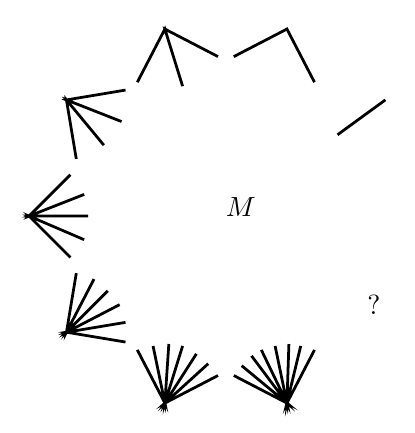
\begin{tikzpicture}[scale=2.5]
        \draw[-,line width=1pt] (0.81,0.59) -- (0.7*0.81,0.7*0.59);
        \draw[-,line width=1pt] (0.31,0.95) -- (0.04, 0.81) -- (0.31,0.95) -- (0.45, 0.68) -- (0.31,0.95);
        \draw[-,line width=1pt] (-0.31,0.95) -- (-0.45, 0.68) -- (-0.31,0.95) -- (-0.22, 0.66) -- (-0.31,0.95) -- (-0.04, 0.81) -- (-0.31,0.95);
        \draw[-,line width=1pt] (-0.81,0.59) -- (-0.76, 0.29) -- (-0.81,0.59) -- (-0.62, 0.36) -- (-0.81,0.59) -- (-0.53, 0.48) -- (-0.81,0.59) -- (-0.51, 0.64) -- (-0.81,0.59);
        \draw[-,line width=1pt] (-1.0,-0.0) -- (-0.79, -0.21) -- (-1.0,-0.0) -- (-0.72, -0.12) -- (-1.0,-0.0) -- (-0.7, -0.0) -- (-1.0,-0.0) -- (-0.72, 0.11) -- (-1.0,-0.0) -- (-0.79, 0.21) -- (-1.0,-0.0);
        \draw[-,line width=1pt] (-0.81,-0.59) -- (-0.51, -0.64) -- (-0.81,-0.59) -- (-0.51, -0.54) -- (-0.81,-0.59) -- (-0.54, -0.45) -- (-0.81,-0.59) -- (-0.6, -0.38) -- (-0.81,-0.59) -- (-0.67, -0.32) -- (-0.81,-0.59) -- (-0.76, -0.29) -- (-0.81,-0.59);
        \draw[-,line width=1pt] (-0.31,-0.95) -- (-0.04, -0.81) -- (-0.31,-0.95) -- (-0.09, -0.75) -- (-0.31,-0.95) -- (-0.15, -0.7) -- (-0.31,-0.95) -- (-0.22, -0.66) -- (-0.31,-0.95) -- (-0.29, -0.65) -- (-0.31,-0.95) -- (-0.37, -0.66) -- (-0.31,-0.95) -- (-0.45, -0.68) -- (-0.31,-0.95);
        \draw[-,line width=1pt] (0.31,-0.95) -- (0.45, -0.68) -- (0.31,-0.95) -- (0.38, -0.66) -- (0.31,-0.95) -- (0.32, -0.65) -- (0.31,-0.95) -- (0.25, -0.66) -- (0.31,-0.95) -- (0.18, -0.68) -- (0.31,-0.95) -- (0.13, -0.71) -- (0.31,-0.95) -- (0.08, -0.76) -- (0.31,-0.95) -- (0.04, -0.81) -- (0.31,-0.95);        
        \GraphInit[vstyle=Welsh]
        \Vertices[]{circle}{0,1,2,3,4,5,6,7,8,$M$}
        \draw (0.6,-0.45) node {?};
        \end{tikzpicture} 
    \end{center}
    \caption{La fiesta de Abril}\label{f5.2}
\end{figure}


\begin{ejemplo*} Mario y su mujer Abril dan una fiesta en la cual hay otras cuatro parejas de casados. Las
parejas, cuando arriban, estrechan la mano a algunas personas, pero, naturalmente, no se estrechan la mano entre marido y mujer. Cuando la fiesta finaliza el profesor pregunta a los otros a cuantas personas han estrechado la mano, recibiendo $9$ respuestas diferentes. ¿Cuántas personas estrecharon la mano de Abril?
\end{ejemplo*}
\begin{proof}[Solución] Construyamos un grafo cuyos vértices son las personas que asisten a la fiesta. Las aristas del grafo son las  $\{x,y\}$ siempre y cuando $x$ e $y$ se hayan estrechado las manos. Puesto que hay nueve personas aparte de Mario, y que una persona puede estrechar a lo sumo a otras $8$ personas, se sigue que las $9$ respuestas diferentes que ha recibido el profesor deben ser $0, 1, 2, 3, 4, 5, 6, 7, 8.$
Denotemos los vértices con estos números y usemos $M$ para Mario. Así obtenemos la representación pictórica de la Fig. \ref{f5.2}

Ahora, el vértice $8$ alcanza a todos los otros vértices excepto uno, el cual debe por lo tanto representar a la esposa de $8$. Este vértice debe ser el $0$ el cual por cierto que no está unido al $8$ (ni ob\-via\-men\-te a ningún otro). Luego $8$ y $0$ son una pareja de casados y $8$ está unido a $1, 2, 3, 4, 5, 6, 7$ y $M$. En particular el $1$ está unido al $8$ y ésta es la única arista que parte del $1$. Por consiguiente $7$ no esta unido al $0$ y al $1$ (únicamente), y la esposa de $7$ debe ser $1$, puesto que $0$ esta casado con $8$. Continuando con este razonamiento vemos que $6$ y $2$, y $5$ y $3$ son parejas de casados. Se sigue entonces que $M$ y $4$ están casados, luego el vértice $4$ representa a Abril, quien estrechó la mano de cuatro personas.
\end{proof}

Aunque la representación pictórica es intuitivamente atractiva para los seres humanos, es claramente inútil cuando deseamos comunicarnos con una computadora. Para lograr esto debemos re\-pre\-sen\-tar el grafo mediante cierta clase de lista o tabla. Diremos que dos vértices $x$ e $y$ de un grafo son \textit{adyacentes} cuando $\{x,y\}$ es una arista. \index{vértices adyacentes} (o también diremos que $x$ e $y$ son \textit{vecinos}).  Entonces podemos representar un grafo $G=(V,E)$ por su \textit{lista de adyacencia},  \index{lista de adyacencia} donde cada vértice $v$ encabeza una lista de aquellos vértices que son adyacentes a $v$. El grafo de Fig. \ref{f5.1} tiene la siguiente lista de adyacencia:

\begin{center}
\begin{tabular}{ccccc}
$a$&$b$&$c$&$d$&$z$ \\ \hline
$b$&$a$&$d$&$a$&$b$ \\
$d$&$z$&&$c$&$d$\\
&&&$z$&
\end{tabular}
\end{center}

Las listas de adyacencia son redundantes (cada arista está representada dos veces) pero como todo lenguaje de programación de alto nivel maneja la estructura tipo lista,  preferimos esta representación pues  un grafo  resulta ser como una lista de listas  o un  arreglo de listas.  


\begin{ejemplo*}
Por cada entero positivo $n$ definimos el \textit{grafo completo  \index{grafo completo} $K_n$} como el grafo con $n$ vértices y en el cual cada par de vértices es adyacente. 

¿Cuántas aristas tiene $K_n$? De cada vértice ``salen'' $n-1$ aristas, las que van a otros vértices. Si  sumamos $n$-veces las $n-1$ aristas es claro que estamos contando cada arista dos veces, luego el número total de aristas es $n(n-1)/2$ (observar que esta es una demostración, usando  grafos, de que $\sum_{i=1}^n i = n(n-1)/2$).
\end{ejemplo*}

\subsection*{$\S$ Ejercicios}
\begin{enumerate}
\item A tres casas $A,B,C$ se les debe conectar el gas, el agua y la electricidad: $G,W,E$. Escribir la lista de adyacencia para el grafo que representa este problema y construir una representación pictórica del mismo. ¿Puede usted encontrar un dibujo en el cual las líneas que representan las aristas no se crucen?
\item Los senderos de un jardín han sido diseñados dándoles forma de \textit{grafo rueda} $W_n$, cuyos vértices son $V=\{0,1,2,\ldots,n\}$ y sus aristas son
$$
\begin{aligned}
\{0,1\},\qquad &\{0,2\},\ldots,\{0,n\}, \\
\{1,2\}.\qquad &\{2,3\},\ldots,\{n-1,n\},\qquad \{n,1\}.
\end{aligned}
$$
Describir una ruta por los senderos de tal forma que empiece y termine en le vértice $0$ y que pase por cada vértice una sola vez. \item  ¿Para cuales valores de $n$ se puede hacer una representación pictórica
de $K_n$ con la propiedad que las líneas que representan las aristas no se corten? 
\item Un \textit{{$3$-ciclo}} en un grafo es un conjunto de tres vértices mutuamente adyacentes. Construir un grafo con cinco vértices y seis aristas que no contenga $3$-ciclos.
\end{enumerate}

\end{section}


\begin{section}{Isomorfismo de grafos} \label{5.2}
En este punto nosotros debemos enfatizar que un grafo esta definido como una entidad matemática abstracta. Es en este contexto que nosotros discutiremos el importante problema de que queremos decir cuando decimos que dos grafos son ``el mismo''.

Claramente lo importante de un grafo no son los nombres con que designamos a los vértices, ni su representación pictórica o cualquier otra representación. La propiedad característica de un grafo es la manera en que los vértices están conectados por aristas. 

Antes de definir isomorfismo de grafos repasaremos el  concepto de función o aplicación biyectiva. Dado  dos conjuntos $X,Y$ diremos que una aplicación $f: X \to Y$ es \textit{biyectiva} si para cada $y \in Y$ existe un  único $x \in X$ tal que $f(x) =y$. Un propiedad importante, de las funciones biyectivas es que $f$ es biyectiva si y sólo sí  $f$ tiene \textit{inversa}, es decir existe $f^{-1}: Y \to X$, tal que $f(f^{-1}(y)) = y$, $\forall \,y \in Y$ y $f^{-1}(f(x)) = x$, $\forall \,x \in X$.

\begin{ejemplo*}
La función  
\begin{align*}
f&: \{1,2,3\}\to\{a,b,c\} \quad \text{definida } f(1) = c, f(2) = b, f(3) = a
\end{align*}
es biyectiva y su  inversa es 
$$
f^{-1}(a) = 3,\;f^{-1}(b) = 2,\;f^{-1}(c) =1.
$$
También es biyectiva la aplicación
\begin{align*}
g&: \{x,y\}\times \{u,w,z\} \to \{1,2,3,4,5,6\} \quad \text{definida } 
\end{align*}
$$
g(x,u)= 1,\, g(x,w) =2,\, g(x,z) =3,\, g(y,u) =4,\, g(y,w) =5,\, g(y,z) =6. 
$$
\end{ejemplo*}

\begin{definicion} Dos grafos $G_1$ y $G_2$ se dicen que son \textit{isomorfos} cuando  existe una biyección $\alpha$ entre el  \index{grafos isomorfos}  \index{isomorfismo de grafos} conjunto de vértices de $G_1$ y el conjunto de vértices de $G_2$ tal que  si $\{x,y\}$ es una arista de $G_1$ entonces $\{\alpha(x),\alpha(y)\}$ es una arista de $G_2$ y recíprocamente si  $\{z,w\}$ es una arista de $G_2$ entonces $\{\alpha^{-1}(z),\alpha^{-1}(w)\}$ es una arista de $G_1$. La biyección $\alpha$ es llamada un \textit{isomorfismo}.
\end{definicion}

Por ejemplo, considere los dos grafos de la Fig. \ref{f5.3}. En este caso hay una biyección entre el conjunto de vértices de $G_1$ y el conjunto de vértices de $G_2$ la cual tiene la propiedad requerida; esta biyección es dada por
$$
\alpha(a)=t,\quad \alpha(b)=v,\quad \alpha(c)=w,\quad \alpha(d)=u.
$$
Podemos comprobar que a cada arista de $G_1$ le corresponde una arista de $G_2$ y vi\-ce\-ver\-sa. Por ejemplo, a la arista $bc$ de $G_1$ le corresponde la arista $vw$ de $G_2$, y así siguiendo. (Usaremos la abreviación $xy$ para la arista $\{x,y\}$, recordando que una arista es un par desordenado, es decir $xy$ es lo mismo que $yx$.)

\begin{figure}[ht]
    \begin{center}
    \begin{tabular}{llll}
        &
        \begin{tikzpicture}[scale=1]
        %\SetVertexSimple[Shape=circle,FillColor=white]
        \Vertex[x=0,y=0]{$a$}
        \Vertex[x=2,y=0]{$b$}
        \Vertex[x=2,y=-2]{$c$}
        \Vertex[x=0,y=-2]{$d$}
        \Edges($a$, $b$,$c$,$d$,$a$,$b$,$d$)
        \draw (1,-3) node {$G_1$};
        \end{tikzpicture}
        &
        \qquad
        & 
        \begin{tikzpicture}[scale=1]
        %\SetVertexSimple[Shape=circle,FillColor=white]
        \Vertex[x=1,y=0]{$t$}
        \Vertex[x=1,y=-1.3]{$w$}
        \Vertex[x=2,y=-2]{$v$}
        \Vertex[x=0,y=-2]{$u$}
        \Edges($v$, $t$,$u$,$v$,$w$,$u$)
        \draw (1,-3) node {$G_2$};
        \end{tikzpicture}
    \end{tabular}
    \end{center}
    \caption{$G_1$ y $G_2$ son isomorfos} \label{f5.3}
\end{figure}

Cuando, como en la Fig. \ref{f5.3}, dos grafos $G_1$ y $G_2$ son isomorfos usualmente nos referiremos a ellos como que son ``el mismo'' grafo. 

Para mostrar que dos grafos no son isomorfos, nosotros debemos demostrar que no hay una biyección entre el conjunto de vértices de uno con el conjunto de vértices de otro, que lleve las aristas de uno en las aristas del otro.

\begin{figure}[ht]
    \begin{center}
\begin{tabular}{llll}
    &
    \begin{tikzpicture}[scale=1]
    %\SetVertexSimple[Shape=circle,FillColor=white]
    \Vertex[x=0.00, y=2.00]{$a$}
    \Vertex[x=1.90, y=0.62]{$b$}
    \Vertex[x=1.18, y=-1.62]{$c$}
    \Vertex[x=-1.18, y=-1.62]{$d$}
    \Vertex[x=-1.90, y=0.62]{$e$}
    \Edges($c$, $b$,$a$,$e$,$d$,$b$,$a$,$d$)
    \Edges($e$,$b$)
    \draw (0,-2.2) node {$G_1$};
    \end{tikzpicture}
    &
    \qquad
    & 
    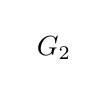
\begin{tikzpicture}[scale=1]
    %\SetVertexSimple[Shape=circle,FillColor=white]
    \Vertex[x=0.00, y=2.00]{1}
    \Vertex[x=1.90, y=0.62]{2}
    \Vertex[x=1.18, y=-1.62]{3}
    \Vertex[x=-1.18, y=-1.62]{4}
    \Vertex[x=-1.90, y=0.62]{5}
    \Edges(1,2,3,4,5,1)
    \Edges(4,2,5)
    \draw (0,-2.2) node {$G_2$};
    \end{tikzpicture}
\end{tabular}
\end{center}
    \caption{$G_1$ y $G_2$ no son isomorfos} \label{f5.4}
\end{figure}

Si dos grafos tienen diferente número de vértices, entonces no es posible ninguna biyección, y los grafos no pueden ser isomorfos. Si los grafos tienen el mismo número de vértices, pero di\-fe\-ren\-te número de aristas, entonces hay biyecciones de vértices  pero ninguna de ellas puede ser un isomorfismo. 

\begin{definicion} 
Sea $G=(V,E)$ un grafo. Se dice que $G^{\prime}=(V^{\prime},E^{\prime})$ es \textit{subgrafo} de
$G=(V,E)$ si $V^{\prime} \subset V$, $E^{\prime} \subset E$ y todos los vértices que son extremos de las aristas de $E^{\prime}$
están en $V^{\prime}$.
\end{definicion}

Es claro, pero  no lo demostraremos aquí, que un isomorfismo lleva un subgrafo a un subgrafo isomorfo. Este resultado es una herramienta que puede ser útil para ver si dos grafos no son isomorfos. 

Por ejemplo, los dos grafos de la Fig. \ref{f5.4} tienen cada uno cinco vértices y siete aristas pero no son isomorfos. Una manera de ver esto es observar que los vértices $a$, $b$, $d$, $e$ forman un subgrafo completo de $G_1$ (cada par de ellos está conectado por una arista). Cualquier isomorfismo debe llevar estos vértices en cuatro vértices de $G_2$ con la misma propiedad, y puesto que no hay tal conjunto de vértices en $G_2$ no puede haber ningún isomorfismo.

\subsection*{$\S$ Ejercicios}\label{ejercicios5.2}
\begin{enumerate}
\item Probar que los grafos mostrados en la Fig. \ref{f5.5} no son isomorfos.
\begin{figure}[ht]
    \begin{center}
    \begin{tabular}{llll}
        &
        \begin{tikzpicture}[scale=1]
        \SetVertexSimple[Shape=circle,FillColor=white,MinSize=8 pt]
        \Vertex[x=0.00, y=2.00]{a}
        \Vertex[x=2., y=-1.50]{b}
        \Vertex[x=-2., y=-1.50]{c}
        \Edges(a,b,c,a)
        \Vertex[x=0.00, y=0.85]{1}
        \Vertex[x=1., y=-0.9]{2}
        \Vertex[x=-1., y=-0.9]{3}
        \Edges(1,2,3,1)
        \Edges(a,1,3,c,b,2)
        \draw (0,-2.2) node {$G_1$};
        \end{tikzpicture}
        &
        \qquad
        & 
        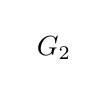
\begin{tikzpicture}[scale=0.65]
        \SetVertexSimple[Shape=circle,FillColor=white,MinSize=8 pt]
        %                
        \Vertex[x=3.00, y=0.00]{1}
        \Vertex[x=1.50, y=2.60]{2}
        \Vertex[x=-1.50, y=2.60]{3}
        \Vertex[x=-3.00, y=0.00]{4}
        \Vertex[x=-1.50, y=-2.60]{5}
        \Vertex[x=1.50, y=-2.60]{6}
        \Edges(1,2,3,4,5,6,1)
        \Edges(1,4) \Edges(3,6) \Edges(2,5)
        \draw (0,-3.8) node {$G_2$};
        \end{tikzpicture}
    \end{tabular}
\end{center}
    \caption{Probar que estos grafos no son isomorfos}\label{f5.5}
\end{figure}

\item \label{ejercicio5.2.2}Encontrar un isomorfismo entre los grafos definidos por las siguientes listas de
adyacencias. (Ambas listas especifican versiones de un grafo famoso conocido como \textit{grafo de Petersen}). \index{grafo dePetersen}
$$
\begin{matrix}
a&b&c&d&e&f&g&h&i&j\\ \hline
b&a&b&c&d&a&b&c&d&e\\
e&c&d&e&a&h&i&j&f&g\\
f&g&h&i&j&i&j&f&g&h
\end{matrix}
\qquad \begin{matrix}
0&1&2&3&4&5&6&7&8&9\\ \hline
1&2&3&4&5&0&1&0&2&6\\
5&0&1&2&3&4&4&3&5&7\\
7&6&8&7&6&8&9&9&9&8
\end{matrix}
$$

\item Sea $G=(V,E)$ el grafo definido como sigue. El conjunto de vértices $V$ es el conjunto de todas las palabras de longitud tres en el alfabeto $\{0,1\}$, y el conjunto de aristas $E$ contiene aquellos pares de palabras que difieren exactamente en una posición. Probar que $G$ es isomorfo al grafo formado por las esquinas y aristas de un cubo.
\end{enumerate}
%\end{subsection}

\end{section}


\begin{section}{Valencias}\label{5.3}
La \textit{{valencia}} de un vértice $v$ en un grafo $G=(V,E)$ es el \index{valencia de un vértice} número de aristas de $G$ que contienen a $v$. Usaremos la notación $\delta(v)$ para la valencia de $v$, formalmente
$$
\delta(v)=|D_v|, \quad \text{ donde } \quad D_v=\{e \in E| v\in
e\}.
$$
El grafo descrito en Fig. \ref{f5.1} tiene $\delta(a)=2$, $\delta(b)=2$, $\delta(c)=1$, $\delta(d)=3$, $\delta(z)=2$. El primer teorema de la teoría de grafos nos dice que la suma de estos números es dos veces el número de aristas.

\begin{teorema}\label{t5.3} La suma de los valores de las valencias $\delta(v)$, tomados sobre todos los vértices $v$ del grafo $G=(V,E)$, es igual a dos veces el número de aristas:
$$
\sum_{v \in V} \delta(v) = 2|E|.
$$
\end{teorema}
\begin{proof} La valencia de un vértice $v$ indica la cantidad de ``extremos'' de aristas que ``tocan'' a $v$. Es claro que hay $2|E|$ extremos de aristas, luego la suma total de las valencias de los vértices es $2|E|$.
\end{proof}

Hay un útil corolario de este resultado. Diremos que un vértice de $G$ es \textit{impar} si su  \index{vértice impar}  \index{vértice par} valencia es impar, y \textit{par} si su valencia es par. Denotemos $V_i$ y $V_p$ los conjuntos de vértices impares y pares respectivamente, luego $V=V_i \cup V_p$ es una partición de $V$. Por teorema \ref{t5.3}, tenemos que
$$
\sum_{v \in V_i} \delta(v) + \sum_{v \in V_p} \delta(v)= 2|E|.
$$
Ahora cada término en la segunda suma es par, luego esta suma es un número par. Puesto que el lado derecho también es un número par, la primera suma debe ser también par. Pero la suma de números impares solo puede ser par si el número de términos es par. En otra palabras:

\begin{teorema} El número de vértices impares es par.
\end{teorema}

Este resultado es a veces llamado el ``handshaking lemma'' (handshake=estrechar la mano, darse la  \index{handshaking lemma} mano), debido a que se puede interpretar en términos de gente y darse la mano: dado un conjunto de personas, el número de personas que le ha dado la mano a un número impar de miembros del conjunto
es par. 

Un grafo en el cual todos los vértices tienen la misma valencia $r$ se llama \textit{regular}  \index{grafo regular} (con valencia $r$), o \textit{$r$-valente.} En este caso, el resultado del teorema \ref{t5.3} se traduce
$$
r|V|=2|E|.
$$

Muchos de los grafos que aparecen en las aplicaciones son regulares. Ya conocemos los  grafos completos $K_n$; ellos son regulares, con valencia $n-1$. De geometría elemental conocemos los polígonos de $n$ lados, los cuales en teoría de grafos son llamados \textit{{grafos cíclicos}}  \index{grafo cíclico} $C_n$. Formalmente, podemos decir que el conjunto de vértices de $C_n$ es $\mathbb Z_n$, y los vértices $i$ y $j$ están unidos si $j=i+1$ o $j=i-1$ en $\mathbb Z_n$. Claramente, $C_n$ es un grafo regular con valencia $2$, si $n\ge 3$.

Una aplicación importante de la noción de valencia es en el problema de determinar si dos grafos son o no isomorfos. Si $\alpha:V_1 \to  V_2$ es un isomorfismo entre $G_1$ y $G_2$, y $\alpha(v)=w$, entonces cada arista que contiene a $v$ se transforma en una arista que contiene a $w$. En consecuencia $\delta(v)=\delta(w)$. Por otro lado, si $G_1$ tiene un vértice $x$, con valencia $\delta(x)=\delta_0$, y $G_2$ no tiene vértices con valencia $\delta_0$, entonces $G_1$ y $G_2$ no pueden ser isomorfos. Esto nos da otra manera para distinguir los grafos de la Fig \ref{f5.4}, puesto que el primer grafo tiene un vértice de valencia 1 y el segundo no.

Una extensión de esta idea se da en la siguiente proposición.

\begin{proposicion}\label{criterioiso}Sean  $G_1$ y $G_2$ grafos isomorfos. Para cada $k\ge 0$ sea $n_i(k)$ el número de vértices de $G_i$ que tienen valencia $k$ ($i=1,2$). Entonces $n_1(k)=n_2(k)$.
\end{proposicion}
\begin{proof} Hemos visto más arriba que si $\alpha:V_1 \to  V_2$ es un isomorfismo entre $G_1$ y $G_2$ y $v\in V_1$, entonces $\delta(v)=\delta(\alpha(v))$. Luego la cantidad de vértices con valencia $k$ en $G_1$ es igual  a la cantidad de vértices con valencia $k$ en $G_2$.     
\end{proof}

\begin{ejemplo*} Revisemos los grafos de la Fig. \ref{f5.4} y la Fig. \ref{f5.5} de la sección anterior. 

Los dos grafos de la Fig. \ref{f5.4}  no son isomorfos debido a que en el primer grafo existen tres vértices con valencia $3$ mientras que en el segundo existen sólo dos.

Observar que los criterios vistos hasta ahora relativos a cantidad de vértices,  cantidad de aristas y valencias, incluyendo el de la proposición \ref{criterioiso}, no son útiles para determinar si los grafos de  la Fig. \ref{f5.5} son isomorfos o no: ambos tienen $6$ vértices, $9$ aristas y todos los vértices son de valencia $3$. Sin embargo, en el caso de la Fig. \ref{f5.5} podemos determinar que los grafos no son isomorfos observando los subgrafos de cada uno. Ahora bien, no  hay ningún criterio general eficiente para determinar si dos grafos son isomorfos o no: en los casos difíciles esencialmente debemos probar con todas las biyecciones posibles de los vértices de un grafo a los vértices del otro y eso es no computable para casos no demasiado  grandes.   
\end{ejemplo*}

\subsection*{$\S$ Ejercicios}\label{ejercicios5.3}
\begin{enumerate}
\item ¿Es posible que las siguientes listas sean las valencias de todos los vértices de un grafo? Si así lo fuera, dar una representación pictórica de tal grafo. (Recordar que hay a lo más una arista que una un par de
vértices dados.)
\begin{multicols}{2}
    \begin{enumerate}
        \item $2,2,2,3.$
        
        \item $1,2,2,3,4.$
        
        \item $2,2,4,4,4.$
        
        \item $1,2,3,4.$
    \end{enumerate}
\end{multicols}

\item Si $G=(V,E)$ es un grafo, el \textit{complemento}\index{complemento de un grafo} $G^c$ de $G$ es el grafo cuyo conjunto de vértices es $V$ y cuyas aristas unen aquellos vértices que no son unidos por $G$. Si $G$ tiene $n$ vértices y sus valencias son $d_1,d_2,\ldots,d_n$, ¿cuáles son las valencias de $G^c$? 

\item Encuentrar todos los grafos posibles (no isomorfos) que pueda, que sean regulares, $4$-valentes y con $7$ vértices. [Ayuda: considere el complemento de esos grafos.]

\item Probar que si $G$ es un grafo con al menos dos vértices, entonces $G$ tiene dos vértices con la misma valencia.
\end{enumerate}

\end{section}


\begin{section}{Caminos y ciclos}\label{5.4}

Frecuentemente usamos grafos como modelos de situaciones prácticas que involucran rutas: los vértices representan ciudades o cruces, y cada arista representa una ruta o cualquier otro forma de comunicación. Las definiciones de esta sección se comprenderán mejor con esta clase de ejemplo en mente.

\begin{definicion}  Una \textit{caminata} en un grafo $G$ es  \index{caminata} una secuencia de vértices
$$
v_1,v_2,\ldots,v_k,
$$
tal que $v_i$ y $v_{i+1}$ son adyacentes ($1 \le i \le k-1$). Si todos los vértices son distintos, una caminata es llamada un \textit{camino}.  \index{camino}

Llamaremos \textit{ciclo} a una caminata \index{ciclo} $v_1,v_2,\ldots,v_{r+1}$  con $r \ge 3$ y cuyos vértices son distintos exceptuando los extremos, es decir que $v_1,v_2,\ldots,v_{r}$ es un camino de al menos tres vértices y $v_1=v_{r+1}$.  A menudo diremos que es un \textit{$r$-ciclo}, o un ciclo de \textit{longitud} $r$ en $G$.  \index{longitud de un ciclo}
\end{definicion}

Es decir, una caminata especifica una ruta en $G$: del primer vértice vamos a uno adyacente, de éste a otro adyacente y así siguiendo. En una caminata podemos visitar cualquier vértice varias veces, y en particular, podemos ir de un vértice $x$ a otro $y$ y luego tomar la dirección contraria y regresar a $x$. En un camino, cada vértice es visitado solo una vez.

Escribamos $x \sim y$ siempre y cuando los vértices $x$ e $y$ de $G$ puedan ser unidos por un camino en $G$: hablando en forma rigurosa, esto significa que hay un camino $v_1,v_2,\ldots,v_k$ en $G$ con $x=v_1$ e $y=v_k$. 

\begin{lema} Sea $G$ un grafo. $x \sim y$ si  y sólo si $x$ e $y$ pueden ser unidos por una caminata 
\end{lema}
\begin{proof}Es claro que si $x$ e $y$ están unidos por un camino, como  un camino es un caso especial de caminata, $x$ e $y$ están unidos por una caminata.

Veamos que si  $x$ e $y$ están unidos por una caminata, entonces están unidos por un camino. Sea 
$$
x=x_1,x_2,\ldots,x_k=y,
$$
una caminata entre  $x$ e $y$. Si ninguno de los $x_i$ se repite, entonces tenemos un camino y terminado el problema. Si hay repetición, entonces existe $j$ tal que $x_j = x_{j+r}$ con $r >0$, es decir tenemos una caminata
$$
x=x_1,x_2,\ldots,x_j,\ldots,x_{j+r},\ldots, x_k=y,
$$
Como $x_j = x_{j+r}$ podemos eliminar la subcaminata $x_{j+1},\ldots,x_{j+r}$ (un ``bucle'' dentro de la caminata) y nos queda 
$$
x=x_1,x_2,\ldots,x_j,x_{j+r+1},\ldots, x_k=y,
$$
una caminata, más corta,  entre $x$ e $y$. Podemos repetir este procedimiento hasta eliminar todos los ``bucles'' y obtener un camino.
\end{proof}

\begin{definicion} Diremos que un grafo  $G$ es \textit{conexo} si para cualesquiera dos vértices $x,y$ existe una camina de $x$ a $y$, es decir si  $x \sim y$. 
\end{definicion}

Debido al lema que probamos más arriba, es sencillo verificar la siguientes propiedades: sea $G$ grafo y sean $x,y,z$ vértices de $G$, entonces
\begin{enumerate}[label=\textit{\alph*)}]
\item  $x \sim x$ (reflexividad de $\sim$).
\item  $x \sim y$, entonces $y \sim x$ (simetría de $\sim$).
\item  $x \sim y$,  $y \sim z$, entonces  $x \sim z$ (transitividad  de $\sim$).
\end{enumerate}


En un lenguaje formal, una relación que  cumple las tres propiedades anteriores es llamada una  \textit{relación de equivalencia} del conjunto, en este caso tenemos una relación de equivalencia del conjunto de vértices $V$ de $G$. 

Estas tres propiedades nos permiten partir a $V$ en conjuntos disjuntos: dos vértices están en el mismo conjunto si ellos pueden ser unidos por un camino, y están en conjuntos diferentes si no podemos encontrar tal camino. llamaremos a estos conjuntos disjuntos las \textit{clases de equivalencia de $\sim$}.

\begin{definicion}Supongamos que $G=(V,E)$ es un grafo y que la partición de $V$ en las clases de equivalencia de $\sim$ es
$$
V= V_1 \cup V_2 \cup \cdots \cup V_r.
$$
Denotemos con $E_i$ ($1\le i \le r$) al subconjunto de $E$ que contiene todas las aristas cuyos finales están en $V_i$. Entonces los grafos $G_i=(V_i,E_i)$ son llamados las \textit{componentes}  \index{componente de un grafo}  \index{grafo conexo} de $G$. Si $G$ tiene solo una componente entonces, claramente, el grafo es {conexo}.
\end{definicion}

\begin{figure}[t]
    \begin{center}
\begin{tikzpicture}[scale=1.1]
\SetVertexSimple[Shape=circle,FillColor=white,MinSize=8 pt]            
\Vertex[x=6, y=-0.5]{1}
\Vertex[x=5.5, y=-2]{2}
\Vertex[x=7, y=-3.5]{3}
\Vertex[x=7, y=-2]{4}
\Vertex[x=11, y=-2]{5}
\Vertex[x=6.50, y=-1.2]{6}
\Vertex[x=6.50, y=-2.5]{7}
\Vertex[x=9.5, y=-0.8]{8}
\Vertex[x=8.5, y=-2.5]{9}
\Vertex[x=10, y=-3.3]{a}
\Edges(5,1,2,4,5,3,2,4,3,5,4)
\Edges(a,8,9,7,6,8,9)
\end{tikzpicture}
\end{center}
\caption{Un grafo con dos componentes} \label{f5.6}
\end{figure}

La terminología casi explica por si misma el significado de estas definiciones. El grafo mostrado en la Fig. \ref{f5.6} tiene dos componentes, y por consiguiente no es conexo. La descomposición de un grafo en componentes es muy útil, puesto que muchas propiedades de los grafos pueden ser establecidas considerando las componentes separadamente. Por esta razón, teoremas acerca de grafos a menudo son probados solo para la clase de grafos conexos.

Cuando un grafo de moderado tamaño es dado por una representación pictórica es bastante fácil determinar si es o no conexo. Sin embargo, cuando un grafo es dado por una lista de adyacencia necesitaremos un algoritmo eficiente para decidir si es o no conexo. 

\begin{figure}[b]
    \begin{center}
        \begin{tikzpicture}[scale=1]
        %\SetVertexSimple[Shape=circle,FillColor=white]
        \def\rvar{1.2}
        \Vertex[x=0.00, y=-2.00]{$u$}
        \Vertex[x=\rvar*1.90, y=-0.62]{$t$}
        \Vertex[x=\rvar*1.18, y=1.62]{$q$}
        \Vertex[x=-1.18*\rvar, y=1.62]{$p$}
        \Vertex[x=-1.90*\rvar, y=-0.62]{$r$}
        \Vertex[x=0, y=0]{$s$}
        \Edges($u$,$t$,$q$,$p$,$r$,$u$,$s$,$t$,$r$,$s$,$q$,$r$,$p$,$t$,$s$,$u$,$s$,$p$)
        \end{tikzpicture}
    \end{center}
    \caption{El gran tour} \label{f5.7}
\end{figure}

\begin{ejemplo}\label{chunner} Leandro y Juan, dos amigos, planean tomar sus vacaciones en determinada isla. La Fig. \ref{f5.7} representa los lugares de interés turístico de la isla y las carreteras que los unen. Leandro es un turista por naturaleza, y desea visitar cada lugar una vez y volver al punto de partida. Juan es un explorador, y desea atravesar todos los caminos solo una vez, a él lo tiene sin cuidado si regresa o no al lugar del cual partió. ¿Podrán encontrar las rutas que desean Leandro y Juan?
\begin{proof}[Solución] Leandro puede usar diferentes rutas para alcanzar su objetivo: una posibilidad es el ciclo $p,q,t,s,u,r,p$.
    
    Sin embargo, Juan está en un apuro. Llamemos $x$ al punto de partida y llamemos $y$ al punto de llegada, y supongamos por el momento que $x \not= y$. Entonces él usa una arista con extremo en $x$ para partir y cada vez que vuelve a $x$ debe arribar y partir por nuevas aristas. Luego, usa un número impar de aristas con extremo en $x$, y por consiguiente $x$ debe ser un vértice impar. De manera análoga, $y$ debe ser también un vértice impar, puesto que Juan usa dos aristas cada vez que pasa por $y$, y una más al finalizar en $y$. Los restantes vértices deben ser pares, puesto que cada vez que Juan llega a un vértice intermedio parte de nuevo, y por consiguiente usa dos aristas.
    
    Resumiendo, una ruta para Juan que empiece y finalice en vértices distintos $x$ e $y$, es solo posible si hay dos vértices impares (que son $x$ e $y$) y el resto de los vértices es par.  Pero en el grafo de la Fig. \ref{f5.7} el valor de las valencias es: $\delta(p)=4$, $\delta(q)=4$, $\delta(r)=5$, $\delta(s)=5$, $\delta(t)=5$, y $\delta(u)=3$. Luego hay demasiados vértices impares, y por lo tanto no existe la ruta que Juan desea. Si permitimos la posibilidad de que $x=y$ , la situación es aún peor, pues en este caso todos los vértices deberían ser pares.
\end{proof}
\end{ejemplo}

En general, la ruta de Leandro es un ciclo que contiene todos los vértices del grafo dado. Tales ciclos fueron estudiados por el matemático irlandés W.R. Hamilton ($1\,805-65$),  \index{Hamilton, W. R.} y en consecuencia un ciclo con esta propiedad es llamado un \textit{ciclo hamiltoniano}. En nuestro ejemplo, fue muy fácil \index{ciclo hamiltoniano} encontrar un ciclo hamiltoniano, pero este fue un caso muy especial y no representativo. Para ciertos grafos, puede ser un problema difícil decidir si un ciclo hamiltoniano existe o no.

Por otro lado, el problema de Juan puede ser fácilmente resuelto. Una caminata que use cada arista de un grafo solo una vez es llamada una \textit{caminata euleriana}, debido a que Euler \index{caminata euleriana} fue el primero en estudiar estas caminatas y encontró que si $x\not= y$, una condición necesaria para que exista una caminata euleriana que comience en $x$ y finalice en $y$ es que $x$ e $y$ deben ser vértices impares y el resto debe ser par, mientras que si $x=y$ la condición es que todos los vértices deben ser pares. Es decir que una condición necesaria para que exista una caminata euleriana en un grafo $G$
es que $G$ debe tener a lo más dos vértices impares. Más aún, puede probarse que esta condición es también suficiente. Puesto que es sencillo calcular las valencias de los vértices de un grafo, es relativamente sencillo decidir si un grafo tendrá o no una caminata euleriana. 

Resumiendo las definiciones de más arriba:

\begin{definicion}
Un \textit{ciclo hamiltoniano} en un grafo $G$ es un ciclo que contiene a todos los vértices del grafo.

Una \textit{caminata euleriana} en un grafo $G$ es un caminata que usa todas las aristas de $G$ exactamente
una vez. Una caminata euleriana que comienza y termina en un mismo vértice se llama también \textit{circuito euleriano}.
\end{definicion}

El siguiente teorema resume los resultados sobre caminatas eulerianas. La demostración no es demasiada complicada, pero excede los alcances de este curso.  

\begin{teorema}\label{th-caminata-euleriana} Un grafo conexo con más de un vértice posee una caminata euleriana de $v$ a $w$, con $v \not= w$ si y sólo si $v$ y $w$ son los únicos vértices de grado impar. Un grafo conexo con más de un vértice tiene un circuito euleriano si y sólo si todos los vértices tienen grado par.
\end{teorema}

\begin{observacion}\label{obs-par-a-impar}
    El caso de un grafo donde todas las valencias son pares se puede reducir al anterior: si deseamos una caminata euleriana que empiece y termine en $v$, eliminamos una arista del grafo que contenga a $v$, digamos la arista $\{v,w\}$ (con lo cual queda un grafo  con solo dos vértices, $v$ y $w$, de valencia impar), aplicamos el caso  anterior, con lo cual hacemos una caminata euleriana que termina en  $w$, y terminamos la caminata agregando  la arista $\{v,w\}$. 
\end{observacion}

$$
\forall X \subset \mathbb Z \wedge X \ne \emptyset \wedge (\exists a: \forall\, x \in X: a \le x) \Rightarrow (\exists b: \forall, x \in X :b \le x) \wedge (\forall)
$$
\begin{observacion}\label{obs-impar-a-par}
    Análogamente,  el caso de un grafo  $G$ con dos valencias impares y todas las demás valencias pares  se puede reducir al caso en que todas las valencias son pares. Sean $p$ y $q$ los dos vértices de valencia impar,  entonces tenemos dos casos (1) $\{p,q\}$  es arista de $G$ y (2) $\{p,q\}$  no es arista de $G$.  En el caso (1),  eliminamos la arista  $\{p,q\}$  del grafo  y  nos queda un grafo  con todos los vértices de valencia par. Por lo tanto, hay un circuito euleriano de $p$  a $p$. Agregamos al final la arista $\{p,q\}$  y obtenemos una caminata euleriana de  $p$ a $q$. El caso (2) es un poco más complicado: agregamos al grafo $G$ la arista $\{p,q\}$ y obtenemos un grafo  con todos los vértices de valencia par. Luego  hay un circuito euleriano de $q$ a $q$. Podemos describir el circuito como
    $$
    q,v_1,\ldots,v_k,q,p,w_1,\ldots,w_r,q.
    $$
    A partir de este circuito podemos obtener la caminata
    $$
    p,w_1,\ldots,w_r,q,v_1,\ldots,v_k,q, 
    $$
    que es una caminata euleriana. 
\end{observacion}

\subsection*{Algoritmo de Hierholzer}

Más allá del resultado del teorema \ref{th-caminata-euleriana}, existe un algoritmo fácilmente implementable para encontrar circuitos eulerianos.

C. Hierholzer (1840-1871) mostró, poco antes de su muerte, un algoritmo para encontrar un circuito euleriano  para cualquier grafo  con vértices de grado  par.

El  algoritmo es el siguiente: 
\begin{enumerate}
    \item (Paso 1) Elija cualquier vértice  inicial $v$ y haga una caminata  que no repita aristas y  que vuelva al vértice (de $v$ a $v$). No es posible quedarse atascado en ningún vértice que no sea $v$, porque el grado par de todos los vértices garantiza que, cuando se ingresa a un vértice $w$ (distinto de $v$) debe haber una  arista sin usar que nos permite dejar $w$. El recorrido formado de esta manera es un recorrido cerrado, pero puede no cubrir todos los vértices y aristas del grafo inicial.
    \item (Paso iterativo) Mientras exista un vértice $u$ en la caminata ya realizada, pero que tenga aristas que no formen parte de la caminata, inicie otra caminata desde $u$ hasta $u$ siguiendo las aristas no utilizadas. Luego,  inserte esta  caminata a la caminata  anterior para formar una caminata nueva (más larga).
\end{enumerate}

Puesto que suponemos que el grafo original es conexo, repetir el paso iterativo agotará todos las aristas del grafo.

El algoritmo de Hierholzer fue la primera demostración del teorema \ref{th-caminata-euleriana} para el caso  de grafos con vértices de grado par. Obviamente,  debido a la observación  \ref{obs-impar-a-par}, esto demuestra también el teorema para grafos con dos valencias impares.
  
\begin{ejemplo*} Dado  el  grafo de de la  Fig. \ref{f5.7.1}, encontremos una caminata euleriana con origen en $p$ y final en $r$. 

Debemos primero observar que  debe existir un circuito euleriano, pues $\delta(p)=4$, $\delta(q)=4$, $\delta(r)=4$, $\delta(s)=4$,
$\delta(t)=4$, y $\delta(u)=2$,  es decir todos los vértices tienen grado par. 


\begin{figure}[ht]
    \begin{center}
    \begin{tikzpicture}[scale=1]
    %\SetVertexSimple[Shape=circle,FillColor=white]
    \def\rvar{1.2}
    \Vertex[x=0.00, y=-2.00, L=$3$]{$u$}
    \Vertex[x=\rvar*1.90, y=-0.62, L=$2$]{$t$}
    \Vertex[x=\rvar*1.18, y=1.62, L=$1$]{$q$}
    \Vertex[x=-1.18*\rvar, y=1.62, L=$0$]{$p$}
    \Vertex[x=-1.90*\rvar, y=-0.62, L=$4$]{$r$}
    \Vertex[x=0, y=0, L=$5$]{$s$}
    \Edges($u$,$t$,$q$,$p$)
    \Edges($r$,$u$)
    \Edges($s$,$t$)
    \Edges($r$,$s$,$q$,$r$)
    \Edges($p$,$t$,$s$)
    \Edges($s$,$p$,$r$)
    \end{tikzpicture}
    \end{center}
    \caption{El gran tour, de nuevo.} \label{f5.7.1}
\end{figure}

Apliquemos el algoritmo de Hierholzer partiendo  desde $p$. Una caminata posible con origen en $p$ y que vuelva a $p$ es $$p, q, s, r, p.$$

Ahora elijamos $q$ que es un vértice que pertenece a la caminata pero que tiene aristas que no son parte de la caminata. Una caminata que no toca aristas usadas y  que parte de $q$ y regresa a $q$ es $q,r,u,t,q$. Insertamos en $q$  esta caminata  a la caminata anterior y obtenemos:
$$
p,\mathbf{q,r,u,t,q,} s, r, p. 
$$
(En  negrita la caminata insertada).

En  el siguiente paso podemos  elegir $t$ y hacer la caminata $t, p, s, t$ que no pasa por aristas ya utilizadas. Insertamos esta caminata en algún $t$ de la caminata anterior y obtenemos:
$$
p,q,r,u,t, p, s, t,q, s, r, p,
$$
que es un circuito euleriano. 
\end{ejemplo*}



\begin{observacion*}(*) Escribiremos en pseudocódigo el algoritmo para hallar un circuito euleriano en un grafo $G$ con $n$ vértices  de valencia par.
    
Tenemos una grafo $G$ con  $n$ vértices numerados $0,1,\ldots,n-1$,  $G$ se representa por  una lista de adyacencia, es decir $G[i]$  es la lista de vértices adyacentes a $i$.  Tomamos como comienzo del recorrido el vértice arbitrario $0$.

Para no partir el algoritmo en dos páginas, lo incluiremos todo en la página siguiente. 

\newpage
%\vskip .4cm
{%\centering
\begin{minipage}{400pt}
\noindent \textsc{Caminata euleriana } %revisar,  el algoritmo esta cmal
\vskip .2cm
\begin{small}
\begin{verbatim}
# pre: G grafo, 0 vértice de G 
# post: devuelve 'circuito' una lista de vertices que forma una caminata
#       euleriana. La caminata empieza en 0 (y terminará en 0).
circuito = [0]  # caminata
libres = G
# libres representa las aristas no usadas en la caminata 
usados = ista de adyacencia con los vértices de G y sin aristas 
# usados:lista de adyacencia con los vértices de G y sin aristas  
# usados representa las aristas usadas en la caminata
tocados = [0]
# tocados representa los vértices por los cuales pasó la caminata
while enclibr(libres, tocados) != -1:
   # enclibr: listas de adyacencia -> vértices
   # enclibr(libres, tocados) devuelve j en tocados tq libres[j] no es vacío. 
   # En caso contrario, devuelve -1 (representa vacío) 
   pos0 = enclibr(libres, tocados)
   p0 = pos0
   p1 = libres[pos0][0]
   aux = [pos0] # será el circuito a partir de pos0
   while p1 != pos0: # mientras no se vuelva al origen
      aux.append(p1)  # agrega p1 a aux 
      tocados.append(p1)  # agrega p1 a tocados
      quitar_arista(libres, [p0, p1]) # quita de libres la arista 'p0, p1'
      agregar_arista(usados, [p0, p1]) # agregar a usados la arista 'p0, p1'
      p0 = p1 
      p1 = libres[p0][0]
   aux.append(aux[0]) # completa aux a circuito
   quitar_arista(libres, [p0, p1]) # quita de libres la arista 'p0, p1'
   agregar_arista(usados, [p0, p1]) # agregar a usados la arista 'p0, p1'
   inserta_circuito(circuito, aux) # inserta aux en circuito
   pos0 = enclibr(libres, tocados)
return circuito    
\end{verbatim}
\end{small}
\end{minipage}
}
\vskip .4cm
En todo  el programa \texttt{libres} es una lista de adyacencia que nos va dando las aristas no utilizadas. 
Es decir si $w$ es un vértice \texttt{libres[w]} es una lista de los vértices $u$ tal que la arista $wu$ no ha sido utilizada. En forma opuesta,  \texttt{usados} es la lista de las aristas que ya han sida utilizadas. 
\end{observacion*}

\newpage

\subsection*{$\S$ Ejercicios}\label{ejercicios5.4}
%\addcontentsline{toc}{subsection}{Ejercicios}
\begin{enumerate}
\item Encontrar el número de componentes de el grafo cuya lista de adyacencia es
$$
\begin{matrix}
a&b&c&d&e&f&g&h&i&j\\ \hline
f&c&b&h&c&a&b&d&a&a\\
i&g&e&&g&i&c&&f&f\\
j&&g&&&j&e&&&
\end{matrix}
$$

\item ¿Cuántas componentes conexas tiene el grafo de la fiesta de Abril (sección \ref{5.1})?
\item Encontrar un ciclo hamiltoniano en el grafo formado por los vértices y aristas de un
cubo.
\item El año que viene el Leandro y Juan desean visitar otra isla, donde los lugares interesantes y las caminos que los unen están representados por el grafo que tiene la siguiente lista de adyacencia
$$
\begin{matrix}
0&1&2&3&4&5&6&7&8\\ \hline
1&0&1&0&3&0&1&0&1\\
3&2&3&2&5&4&5&2&3\\
5&6&7&4&&6&7&6&5\\
7&8&&8&&8&&8&7.
\end{matrix}
$$
¿Es posible encontrar rutas para Leandro y Juan que satisfagan lo pedido en el ejemplo \ref{chunner}?
\item Un ratón intenta comer un $3\cdot 3\cdot 3$ cubo de queso. Él comienza en una esquina y come un subcubo de $1\cdot 1\cdot 1$, para luego pasar a un subcubo  adyacente. ¿Podrá el ratón terminar de comer el queso en el centro?
\end{enumerate}
%\end{subsection}

\end{section}



\begin{section}{Árboles}\label{5.5}
\begin{definicion} Diremos que un grafo $T$ es un \textit{árbol} si cumple \index{árbol}
\begin{enumerate}
\item[\textbf{T1)}] \label{T1}$T$ es conexo y no hay ciclos en $T$.
\end{enumerate}
\end{definicion}

Algunos árboles típicos han sido dibujados en la Fig. \ref{f5.8}. A causa de su particular estructura y propiedades, los árboles aparecen en diversas aplicaciones de la matemática, especialmente en investigación operativa y ciencias de la computación. Comenzaremos el estudio de ellos estableciendo algunas propiedades sencillas.

\begin{figure}[ht]
    \begin{center}
    \begin{tabular}{llllllll}
        &
        \begin{tikzpicture}[scale=1]
        \SetVertexSimple[Shape=circle,FillColor=white,MinSize=8 pt]
        \Vertex[x=0.00, y=0]{a}
        \Vertex[x=0, y=-1]{b}
        \Vertex[x=0., y=-2]{c}
        \Vertex[x=0, y=-3]{d}
        \Vertex[x=0., y=-4]{e}
        \Edges(a,b,c,d,e)
        \end{tikzpicture}
        &
        \qquad
        & 
        \begin{tikzpicture}[scale=1]
        \SetVertexSimple[Shape=circle,FillColor=white,MinSize=8 pt]
        %                
        \Vertex[x=0.00, y=0]{a}
        \Vertex[x=-1.5, y=-0.5]{b}
        \Vertex[x=1.5, y=-0.5]{c}
        \Vertex[x=-1.5, y=-1.5]{d}
        \Vertex[x=1.5, y=-1.5]{e}
        \Vertex[x=0, y=-1.5]{f}
        \Vertex[x=-0.7, y=-1]{g}
        \Vertex[x=0.7, y=-1]{h}
        \Vertex[x=0, y=-4]{i}
        \Edges(d,b,a,c,e)
        \Edges(g,f,h)
        \Edges(a,f,i)
        \end{tikzpicture}
        &
        \qquad
        & 
        \begin{tikzpicture}[scale=1]
        \SetVertexSimple[Shape=circle,FillColor=white,MinSize=8 pt]
        %                
        \Vertex[x=0.00, y=0]{a}
        \Vertex[x=0, y=-1.0]{b}
        \Vertex[x=0, y=-2.5]{c}
        \Vertex[x=1.2, y=-2]{e}
        \Vertex[x=-1.2, y=-2]{f}
        \Vertex[x=-1.2, y=-3.5]{g}
        \Vertex[x=1.2, y=-3.5]{h}
        \Edges(a,b,c)
        \Edges(f,b,e)
        \Edges(g,c,h)
        \end{tikzpicture}
        &
        \qquad
        & 
        \begin{tikzpicture}[scale=0.65]
        \SetVertexSimple[Shape=circle,FillColor=white,MinSize=8 pt]
        %
        \Vertex[x=0.00, y=0.00]{0}
        \Vertex[x=3.00, y=0.00]{1}
        \Vertex[x=2.12, y=2.12]{2}
        \Vertex[x=0.00, y=3.00]{3}
        \Vertex[x=-2.12, y=2.12]{4}
        \Vertex[x=-3.00, y=0.00]{5}
        \Vertex[x=-2.12, y=-2.12]{6}
        \Vertex[x=0.00, y=-3.00]{7}
        \Vertex[x=2.12, y=-2.12]{8}
        \Edges(1,0,5) \Edges(3,0,7) \Edges(2,0,6)\Edges(4,0,8)
        \end{tikzpicture}
    \end{tabular}
\end{center}
    \caption{Algunos árboles} \label{f5.8}
\end{figure}

El siguiente lema nos resultará útil para probar una parte del teorema fundamental de esta sección.

\begin{lema}\label{conv} Sea $G=(V,E)$ un grafo conexo, entonces $|E| \ge |V| -1$.  
\end{lema}
\begin{proof} Como $G$ es conexo existe una caminata que recorre todos los vértices de $G$:
$$
v_1,v_2,\ldots,v_r.
$$
Renombremos los vértices de $G$ con números naturales de tal forma que el primer vértice de la caminata sea $1$, el segundo $2$ y cada vez que aparece un vértice que no ha sido renombrado se le asigna el número siguiente. Luego la caminata comienza en 1 y termina en $n$, donde $n = |V|$.  Observar que cada vez que renombramos un vértice (excepto el primero) su antecesor es menor, es decir dado $i$ tal que $1 < i \le n$ tenemos que la caminata tiene la forma
$$
1,\ldots,j_i,i,\ldots,j_n,n
$$ 
donde $j_i < i$, luego es claro  que 
$$
\{j_{2},2\}, \{j_{3},3\}, \ldots, \{j_{n},n\}
$$
forman un conjunto de $n-1$ aristas distintas en $G$. 
\end{proof}

\begin{teorema}\label{t5.5} Si $T=(V,E)$ es un grafo conexo con al menos dos vértices, entonces son equivalentes las siguientes propiedades
\begin{enumerate}
\item[\textbf{T1)}] T es un árbol.
\item[\textbf{T2)}] \label{T2} Para cada par $x$, $y$ de vértices existe un único camino en $T$ de $x$ a
$y$.
\item[\textbf{T3)}] \label{T3} El grafo obtenido de $T$ removiendo alguna arista tiene dos
componentes, cada una de las cuales es un árbol.
\item[\textbf{T4)}] \label{T4} $|E|=|V|-1$.
\end{enumerate}
\end{teorema}
\begin{proof}
    \
    
\noindent (T1 $\Rightarrow$ T2) Puesto que $T$ es conexo, existe un
camino de $x$ a $y$, digamos
$$
x=v_0,v_1,\ldots,v_r=y.
$$
Si existiera otro camino, digamos
$$ x=u_0,u_1,\ldots,u_s=y,
$$
consideremos $i$ el más pequeño subíndice para el cual se cumple
que $u_{i+1}\not=v_{i+1}$ Fig. \ref{f5.9}.

\begin{figure}[ht]
    \begin{center}
    \begin{tikzpicture}[scale=1]
    \SetVertexSimple[Shape=circle,FillColor=white,MinSize=5 pt]
    %
    %\ponertz{-7}{-30}{$x=$}
    \draw (-0.6,0) node {$x = $};                
    \draw (0,0.4) node {$v_0$};
    \draw (0,-0.4) node {$u_0$};
    \Vertex[x=0.00, y=0]{v0}
    \Vertex[x=1, y=0]{v1}
    \draw (1,0.4) node {$v_1$};
    \draw (1,-0.4) node {$u_1$};
    \Vertex[x=3, y=0]{vi}
    \draw (2.9,0.4) node {$v_i$};
    \draw (2.9,-0.4) node {$u_i$};
    \Vertex[x=3.7, y=1]{vi1}
    \draw (3.7,1.4) node {$v_{i+1}$};
    \Vertex[x=3.7, y=-1]{ui1}
    \draw (3.7,-1.4) node {$u_{i+1}$};
    \Edges(v0,v1)
    \Edges(vi,vi1)
    \Edges(vi,ui1)
    \Vertex[x=6, y=1]{vj1}
    \draw (6,1.4) node {$v_{j-1}$};
    \Vertex[x=6, y=-1,style=white]{uk1}
    \draw (6,-1.4) node {$u_{k-1}$};
    \Vertex[x=6.7, y=0]{vj}
    \draw (6.8,0.4) node {$v_j$};
    \draw (6.8,-0.4) node {$u_k$};
    \Vertex[x=8.7, y=0]{vr}
    \draw (8.7,0.4) node {$v_r$};
    \draw (8.7,-0.4) node {$u_s$};
    \Edges(vj1,vj)
    \Edges(uk1,vj)
    \draw (9.3,0) node {$=y$};
    
    \SetVertexNormal[LineColor=white]
    \Vertex[x=1.8, y=0]{s1}
    \Vertex[x=2.2, y=0]{s2}
    \Edges(v1,s1)
    \Edges(vi,s2)
    \draw (1.7,0) node {$\scriptstyle\bullet$};
    \draw (2,0) node {$\scriptstyle\bullet$};
    \draw (2.3,0) node {$\scriptstyle\bullet$};
    \Vertex[x=4.5, y=1]{s11}
    \Vertex[x=4.5, y=-1]{s12}
    \Edges(vi1,s11)
    \Edges(ui1,s12)
    \Vertex[x=5.2, y=1]{s21}
    \Vertex[x=5.2, y=-1]{s22}
    \Edges(vj1,s21)
    \Edges(uk1,s22)
    \draw (4.45,1) node {$\scriptstyle\bullet$};
    \draw (4.85,1) node {$\scriptstyle\bullet$};
    \draw (5.25,1) node {$\scriptstyle\bullet$};
    \draw (4.45,-1) node {$\scriptstyle\bullet$};
    \draw (4.85,-1) node {$\scriptstyle\bullet$};
    \draw (5.25,-1) node {$\scriptstyle\bullet$};
    \Vertex[x=7.5, y=0]{s31}
    \Vertex[x=7.9, y=0]{s32}
    \Edges(vj,s31)
    \Edges(vr,s32)
    \draw (7.4,0) node {$\scriptstyle\bullet$};
    \draw (7.7,0) node {$\scriptstyle\bullet$};
    \draw (8.0,0) node {$\scriptstyle\bullet$};
    \end{tikzpicture}
    \end{center}
    %fig 5.10
    \caption{Dos caminos diferentes determinan un ciclo} \label{f5.9}
\end{figure}



Puesto que ambos caminos finalizan en $y$ ellos se encontrarán de nuevo, y entonces podemos definir $j$ como el más pequeño subíndice tal que
$$
j>i \quad \text{ y } \quad v_j=u_k \quad \text{ para algún } k.
$$
Entonces $v_i,v_{i+1},\ldots,v_j,u_{k-1},u_{k-2},\ldots,u_{i+1},v_i$ es un ciclo en $T$, y esto contradice a las hipótesis. Por consiguiente solo existe un camino en $T$ de $x$ a $y$.

%\vskip .2cm 

\noindent (T2 $\Rightarrow$ T3) Supongamos que $uv$ es una arista en $T$, y sea $S=(V,E')$ el grafo con el mismo conjunto de vértices que $T$ y con el conjunto de aristas $E'=E-uv$. Sea $V_1$ el conjunto de los vértices $x$ de $T$ para los cuales existe un único camino en $T$ de $x$ a $v$ que pasa por $u$. Claramente, este camino debe finalizar con la arista $uv$, pues sino $T$ tendría un ciclo. Sea $V_2$ el complemento de
$V_1$ en $V$.

Cada vértice en $V_1$ se une por un camino en $S$ a $u$, y cada vértice en $V_2$ se une por un camino en $S$ a $v$, pero no existe camino de $u$ a $v$ en $S$. Se sigue entonces que $V_1$ y $V_2$ son las dos componentes del conjunto de vértices de $S$. Cada componente es conexa (por definición), y no contiene ciclos, pues sino habría ciclos en $T$. Es decir que las dos componentes son árboles.

%\vskip .2cm 

\noindent(T3 $\Rightarrow$ T4) El resultado es cierto cuando $|V|=1$, puesto que el árbol de un vértice no tiene aristas.

Supongamos que es cierto para árboles con $k$ o menos vértices. Sea $T$ un árbol con $|V|=k+1$, y sea $uv$ una arista en $T$. Si $T_1=(V_1,E_1)$ y $T_2=(V_2,E_2)$ son los árboles que se obtienen removiendo $uv$ en $T$, tenemos que 
$$
|V_1| + |V_2| = |V|, \qquad |E_1| + |E_2| = |E|-1.
$$
Aplicando la hipótesis inductiva a $T_1$ y $T_2$ obtenemos
$$
|E|=|E_1| + |E_2| + 1 = |V_1|-1 +|V_2|-1+1= |V| -1,
$$
como nosotros deseábamos. Por consiguiente el resultado es cierto para todos lo enteros positivos.

\noindent (T4 $\Rightarrow$ T1) Supongamos que $T$ satisface (T4) pero no es árbol. Por lo tanto $T$ tiene al menos un ciclo. Si eliminamos una arista del ciclo, el grafo sigue siendo conexo, pero con una arista menos (y la misma cantidad de vértices), es decir obtenemos un grafo $G' = (V',E')$  conexo y con $|E'| = |V'|-2$. Pero esto contradice el resultado obtenido en el lema \ref{conv}.    
\end{proof}

Las propiedades (T2)-(T3)-(T4) nos dan maneras alternativas de definir árboles. Por ejemplo la propiedad (T2) puede ser considerada como la propiedad que define un árbol, en vez de (T1). 

\begin{observacion*}
El teorema anterior nos muestra un recurso muy usado para probar que una cierta cantidad de afirmaciones son equivalentes. En el caso de $3$ afirmaciones $P$, $Q$, $R$, uno debería probar
$$
P \Leftrightarrow Q,\qquad P \Leftrightarrow R,\qquad Q \Leftrightarrow R,
$$
y eso nos garantizaría la equivalencia entre $P$, $Q$ y $R$. Si embargo, podemos ahorrar trabajo demostrando solamente
$$
P \Rightarrow Q,\qquad Q \Rightarrow R,\qquad R \Rightarrow P,
$$  
pues si queremos probar, por ejemplo $P \Leftrightarrow Q$, esto es equivalente a probar $P \Rightarrow Q$, ya sabido por hipótesis, y $Q \Rightarrow P$, que se deduce de $Q \Rightarrow R$, $R \Rightarrow P$ y la propiedad transitiva de $\Rightarrow$. 

Para el caso de cuatro proposiciones $P_1,P_2,P_3,P_4$ la economía de demostraciones es aún más drástica: para probar todas las equivalencias posibles de cuatro afirmaciones hacen falta 12 demostraciones (seis de ida y seis vuelta), pero alcanza haciendo sólo 4 demostraciones:
$$
P_1 \Rightarrow P_2,\qquad P_2 \Rightarrow P_3,\qquad P_3 \Rightarrow P_4,\qquad P_4 \Rightarrow P_1. 
$$ 
\end{observacion*}

\subsection*{$\S$ Ejercicios}\label{ejercicios5.5}
\begin{enumerate}
\item \label{ejercicio5.5.1} Hay seis diferentes (es decir, no isomorfos entre si) árboles con
seis vértices: hacer un dibujo de ellos.
\item Sea $T=(V,E)$ un árbol con $|V| \ge 2$. Usando la propiedad (T4) y el teorema
\ref{t5.3}
probar que $T$ tiene al menos dos vértices con valencia $1$.
\item Una \textit{foresta} es un grafo que satisface que no contiene ciclos pero no
necesariamente es conexo. Probar que si $F=(V,E)$ es una foresta con
$c$ componentes entonces
$$
|E|=|V|-c.
$$
\end{enumerate}

\end{section}


\begin{section}{Coloreando los vértices de un grafo} \label{5.6}

Un problema que se nos presenta frecuentemente en la vida moderna es aquel de confeccionar un horario para un conjunto de eventos de tal manera de evitar interferencias. Consideremos ahora un caso muy simple, que nos servirá de ejemplo para mostrar como la teoría de grafos puede ayudar al estudio de este problema.

Supongamos que deseamos hacer un horario con seis cursos de una hora, $v_1,v_2,v_3,v_4,v_5,v_6$. Entre la audiencia potencial hay gente que desea asistir a $v_1$ y $v_2$, $v_1$ y $v_4$, $v_3$ y $v_5$, $v_2$ y $v_6$, $v_4$ y $v_5$, $v_5$ y $v_6$ y $v_1$ y $v_6$. ¿Cuántas horas son necesarias para poder confeccionar un horario en el cual no haya interferencias?

Podemos representar la situación por un grafo Fig. \ref{f5.10}. Los vértices corresponden a las seis clases, y las aristas indican las interferencias potenciales.

\begin{figure}[ht]
    \begin{center}
    \begin{tikzpicture}[scale=0.55]
        %\SetVertexSimple[Shape=circle,FillColor=white]
        %                
        \Vertex[x=3.00, y=0.00]{$v_3$}
        \Vertex[x=1.50, y=2.60]{$v_2$}
        \Vertex[x=-1.50, y=2.60]{$v_1$}
        \Vertex[x=-3.00, y=0.00]{$v_6$}
        \Vertex[x=-1.50, y=-2.60]{$v_5$}
        \Vertex[x=1.50, y=-2.60]{$v_4$}
        \Edges($v_2$,$v_1$,$v_6$, $v_5$,$v_4$,$v_1$)
        \Edges($v_2$,$v_6$)
        \Edges($v_3$,$v_5$)
    \end{tikzpicture}
    \end{center}
    %fig 5.10
\caption{El grafo para un problema de horarios} \label{f5.10}
\end{figure}

Un horario el cual cumple con la condición de evitar interferencias es el siguiente:
$$
\begin{matrix}
\text{Hora 1} & \text{Hora 2} &\text{ Hora 3}& \text{Hora 4} \\
v_1 \text{ y } v_3 & v_2 \text{ y } v_4 & v_5 & v_6
\end{matrix}
$$
En términos matemáticos, tenemos una partición del conjuntos de vértices en cuatro partes, con la propiedad que ninguna parte contiene un par de vértices adyacentes del grafo. Un descripción más gráfica utiliza la función 
$$
c: \{ v_1,v_2,v_3,v_4,v_5,v_6\} \to  \{1,2,3,4\}
$$
la cual asigna cada vértice (curso) a la hora que le corresponde. Usualmente, nosotros hablamos de colores asignados a los vértices, en vez de horas, pero claramente la naturaleza exacta de los objetos $1,2,3,4$ no es importante. Podemos usar el nombre de colores reales, rojo, verde, azul , amarillo, o podemos hablar del
color $1$, color $2$, etc. Lo importante es que los vértices que son adyacentes en el grafo deben tener diferentes colores.

\begin{definicion} Una \textit{coloración de vértices} de un  \index{coloración de vértices} grafo $G=(V,E)$ es una función $c:V \to  \mathbb N$ con la siguiente propiedad:
$$
c(x)\not= c(y) \quad \text{ si } \quad \{x,y\} \in E.
$$
El \textit{número cromático} de $G$, denotado $\chi(G)$, se define \index{número cromático} como el mínimo entero $k$ para el cual existe una coloración de vértices de $G$ usando $k$-colores. En otra palabras, $\chi(G)=k$ si  y sólo si existe una coloración de vértices $c$ la cual es una función de $V$ a $\mathbb N_k$, y $k$ es el mínimo entero con esta propiedad. 
\end{definicion}

Volviendo al ejemplo de la Fig. \ref{f5.10}, vemos que nuestro primer intento de horario es equivalente a una coloración de vértices con cuatro colores. El mínimo número de horas necesarias será el número cromático del grafo, y la pregunta es ahora si este número es cuatro o menor que cuatro. Un rápido intento con tres
colores nos da la solución de este problema: 
$$
\begin{matrix}
\text{Color 1}\quad &\text{Color 2}\quad&\text{Color 3} \\
v_1 &v_2 \text{ y } v_5 \quad & v_3,v_4 \text{ y } v_6 .
\end{matrix}
$$
Más aún, hacen falta por lo menos tres colores, puesto que $v_1$, $v_2$, y $v_6$ son mutuamente adyacentes y por lo tanto deben tener diferentes colores. Luego concluimos que el número cromático del grafo es $3$.

En general, para probar que el número cromático de un grafo dado es $k$, debemos hacer dos cosas:
\begin{enumerate}[label=\textit{\alph*)}] 
    \item  encontrar una coloración de vértices usando $k$ colores;
    \item  probar que ninguna coloración de vértices usa menos de $k$ colores.
\end{enumerate}

\subsection*{$\S$ Ejercicios}\label{ejercicios5.6}
\begin{enumerate}
\item \label{ejercicio5.6.1} Encontrar el número cromático de los siguientes grafos:
\begin{enumerate}
    \item un grafo completo $K_n$;
    
    \item un grafo cíclico $C_{2r}$ con un número par de vértices;
    
    \item un grafo cíclico $C_{2r+1}$ con un número impar de vértices.
\end{enumerate}

\item  Determinar los números cromáticos de los grafos descritos en la Fig. \ref{f5.11}.
\begin{figure}[ht]
    \begin{center}
\begin{tabular}{llllll}
    & 
    \begin{tikzpicture}[scale=0.50]
    \SetVertexSimple[Shape=circle,MinSize=5 pt,FillColor=white]
    %
    \Vertex[x=0.00, y=0.00]{0}
    \Vertex[x=3.00, y=0.00]{1}
    \Vertex[x=2.12, y=2.12]{2}
    \Vertex[x=0.00, y=3.00]{3}
    \Vertex[x=-2.12, y=2.12]{4}
    \Vertex[x=-3.00, y=0.00]{5}
    \Vertex[x=-2.12, y=-2.12]{6}
    \Vertex[x=0.00, y=-3.00]{7}
    \Vertex[x=2.12, y=-2.12]{8}
    \Edges(1,0,5) \Edges(3,0,7) \Edges(2,0,6)\Edges(4,0,8)
    \Edges(1,2,3,4,5,6,7,8,1)
    \end{tikzpicture}
    &
    \qquad\quad
    & 
    \begin{tikzpicture}[scale=0.8]
    \SetVertexSimple[Shape=circle,MinSize=5 pt,FillColor=white]
    \Vertex[x=0.00, y=0]{0}
    \Vertex[x=0.00, y=2.00]{1}
    \Vertex[x=1.90, y=0.62]{2}
    \Vertex[x=1.18, y=-1.62]{3}
    \Vertex[x=-1.18, y=-1.62]{4}
    \Vertex[x=-1.90, y=0.62]{5}
    \Edges(1,2,3,4,5,1)
    \Vertex[x=0, y=0.62]{a}
    \Vertex[x=-0.59, y=0.19]{b}
    \Vertex[x=0.59, y=0.19]{c}
    \Vertex[x=-0.36, y=-0.49]{d}
    \Vertex[x=0.36, y=-0.49]{e}
    \Edges(5,d,3,c,1,b,4,e,2,a,5)
    \Edges(0,a)
    \Edges(0,b)
    \Edges(0,c)
    \Edges(0,d)
    \Edges(0,e)
    \end{tikzpicture}
    &
    \qquad\quad
    &     
    \begin{tikzpicture}[scale=0.55]
    \SetVertexSimple[Shape=circle,MinSize=5 pt,FillColor=white]
    %                
    \Vertex[x=3.00, y=0.00]{1}
    \Vertex[x=1.50, y=2.60]{2}
    \Vertex[x=-1.50, y=2.60]{3}
    \Vertex[x=-3.00, y=0.00]{4}
    \Vertex[x=-1.50, y=-2.60]{5}
    \Vertex[x=1.50, y=-2.60]{6}
    \Edges(1,2,3,4,5,6,1)
    \Edges(1,3) \Edges(1,4) \Edges(1,5)
    \Edges(3,5,6,2)
    \end{tikzpicture}
\end{tabular}
\end{center}
    \caption{Encontrar el número cromático}\label{f5.11}
\end{figure}

\item Describir todos los grafos $G$ tales que $\chi(G)=1$.
\end{enumerate}

\end{section}


\begin{section}{El algoritmo greedy para coloración de vértices}
\label{5.7}

Es bastante difícil encontrar el número cromático de un grafo dado. En realidad, no se conoce ningún algoritmo para este problema que trabaje en ``tiempo polinomial'', y la mayoría de la gente cree que tal algoritmo no existe. Sin embargo hay un método simple de hacer una coloración cromática usando un  ``razonable'' número de colores.

El método consiste en asignar los colores de los vértices en orden, de tal manera que cada vértice recibe el primer color que no haya sido ya asignado a alguno de sus vecinos. En este algoritmo insistimos en hacer la mejor elección que podemos en cada paso, sin mirar más allá para ver si esta elección nos traerá problemas luego. Un algoritmo de esta clase se llama a menudo un \textit{algoritmo greedy (goloso)}.  \index{algoritmo greedy (goloso)}

El algoritmo greedy para coloración de vértices es fácil de programar. Supóngase que hemos dado a los vértices algún orden $v_1,v_2,\ldots,v_n$. Asignemos el color $1$ a $v_1$; para cada $v_i$ ($2\le i \le n$) formamos el conjunto $S$ de colores asignados a los vértices $v_j$ ($1\le j <i$) que son adyacentes a
$v_i$, y le damos a $v_i$ el primer color que no está en $S$. (En la práctica, pueden ser usados métodos más sofisticados de manejar los datos.)

\vskip .5cm

\begin{minipage}{400pt}
\noindent \textsc{Algoritmo greedy para coloración de vértices }
\vskip .2cm
\begin{small}
\begin{verbatim}
# pre: 1,...,n los vértices de un grafo G
# post: devuelve v[1],...,v[n] una coloración de G
v[1] = 1 # asignamos el color 1 al vértice 1
for i = 2 to n:
    S = []  # S conjunto de colores asignados a los vértices j
            # (1 <= j <i) que son adyacentes a i (comienza vacío)
    for j = 1 to i-1:
        if j es adyacente a i:
           S.append(v[j])  # agrega el color de j a  S
    k=1
    while k in S:
        k = k+1
    v[i] = k  # Asigna el color k a i, donde k es el primer color que 
              # no esta en S. 
\end{verbatim}
\end{small}
\end{minipage}

\vskip .5cm


Debido a que la estrategia greedy es corta de vista, el número de colores que usará será normalmente más grande que le mínimo posible. Por ejemplo, el algoritmo greedy aplicado en el grafo de Fig. \ref{f5.10} da precisamente le coloración de vértices con cuatro colores que fue propuesta anteriormente, luego encontramos
otra coloración con tres colores. Por supuesto todo depende del orden que se elige inicialmente para los vértices. Es bastante fácil ver que si se elige el orden correcto, entonces el algoritmo greedy nos da la mejor coloración posible (ejercicio \ref{ejercicio5.7}-(2)). Pero hay $n!$ órdenes posibles, y si tuviéramos que controlar cada uno de ellos, el algoritmo requeriría ``tiempo exponencial''.

Más allá de esto, el algoritmo greedy es útil tanto en la teoría como en la práctica. Probaremos ahora dos teoremas por medio de la estrategia greedy.

\begin{teorema}\label{t5.7.1} Si $G$ es un grafo con valencia máxima
$k$, entonces
\begin{enumerate}[label=\textit{\alph*)}]
\item\label{it.com_a}  $\chi(G)\le k+1$,
\item\label{it.com_b} Si $G$ es conexo y no regular , $\chi(G) \le k$.
\end{enumerate}
\end{teorema}
\begin{proof}
    
    \

\ref{it.com_a} Sea $v_1,v_2,\ldots,v_n$ un ordenamiento de los vértices de $G$. Cada vértice tiene a lo más $k$ vecinos, y por consiguiente el conjunto $S$ de los colores asignados por el algoritmo greedy a los vértices $v_j$ que son adyacentes a $v_i$ ($1\le j <i$) tiene como máximo cardinal $k$. Por consiguiente al
menos uno de los colores $1,2,\dots,k+1$ no está en $S$, y el algoritmo greedy asigna entonces el primero de estos a $v_i$.

\ref{it.com_b} Para probar esta parte debemos elegir un orden especial de los vértices, comenzando con $v_n$ y yendo hacia atrás. Puesto que $G$ tiene valencia máxima $k$ y es no regular, existe al menos un vértice $G$ cuya valencia es menor que $k$: llamémoslo $v_n$. Listemos los vecinos de $v_n$ como
$v_{n-1},v_{n-2},\ldots,v_{n-r}$; hay a lo más $k-1$ de ellos. A continuación listemos los vecinos de $v_{n-1}$ (excepto $v_n$ y sus vecinos), y observemos que como la valencia es a lo más $k$ hay a lo más $k-1$ de estos vértices. A continuación listemos los vecinos de $v_{n-2}$ que no hayan sido listados antes, y así
siguiendo. Puesto que $G$ es conexo, en determinado momento podremos listar todos los vértices de $G$. Más aún, el método de construcción asegura que cada vértice es adyacente a lo más a $k-1$ de sus predecesores en el orden $v_1,v_2,\ldots,v_n$.

Usando el mismo argumento que en la parte \ref{it.com_a} (pero para este orden) se sigue que el algoritmo greedy requerirá a lo más $k$ colores. Luego $\chi(G)\le k$. 
\end{proof}

La parte \ref{it.com_b} del teorema es falsa si permitimos que $G$ sea regular. El lector que haya respondido correctamente al ejercicio \ref{ejercicios5.6} \ref{ejercicio5.6.1} será capaz de dar dos ejemplos de este hecho: los grafos completos, y los grafos cíclicos de longitud impar, ambos requieren $k+1$ colores. Si
embargo, puede ser demostrado que estos son los únicos contraejemplos.

Otra consecuencia útil del algoritmo greedy se refiere a grafos $G$ son $\chi(G)=2$. Para tales grafos, los conjuntos $V_1$ y $V_2$ de vértices de colores $1$ y $2$ respectivamente, forman una partición de $V$, con la propiedad que cada arista tiene un vértice en $V_1$ y el otro en $V_2$. Por esta razón, cuando $\chi(G)=2$, diremos que $G$ es \textit{bipartito}. \index{grafo bipartito} Una coloración de vértices con dos colores de un cubo se ilustra en la Fig. \ref{f5.12}, junto a un dibujo alternativo que enfatiza la naturaleza bipartita del grafo. Usualmente usaremos esta clase de dibujo cuando trabajemos con grafos bipartitos.

\begin{figure}[ht]
    \renewcommand{\varx}{1} % variable para cambiar coordenada x
    \renewcommand{\vary}{1} % variable para cambiar coordenada y
    \renewcommand{\varc}{1}
    \begin{center}
    \begin{tabular}{llll}
        & 
        \begin{tikzpicture}[scale=1]
        \SetVertexSimple[Shape=circle,MinSize=5 pt,FillColor=white]
        \Vertex[x=0.00, y=0.00]{0}
        \Vertex[x=2.00, y=0.00]{1}
        \Vertex[x=2.00, y=-2.00]{2}
        \Vertex[x=0.00 , y=-2.00]{3}
        \Vertex[x=0.00 + \varx, y=0.00 + \vary]{4}
        \Vertex[x=2.00 + \varx, y=0.00 + \vary]{5}
        \Vertex[x=2.00 + \varx, y=-2.00 + \vary]{6}
        \Vertex[x=0.00 + \varx, y=-2.00 + \vary]{7}
        \Edges(0,1,2,3,0,4,5,6,7,4)
        \Edges(1,5)
        \Edges(2,6)
        \Edges(3,7)
        \draw (-0.4,0) node {1};
        \draw (-0.4,-2) node {2};
        \draw (-0.4 + \varx, 0.00 + \vary) node {2};
        \draw (-0.4 + \varx,-2.00 + \vary) node {1};
        \draw (2.40, 0.00) node {2};
        \draw (2.40, -2.00) node {1};
        \draw (2.30 + \varx, 0.00 + \vary) node {1};
        \draw (2.30 + \varx, -2.00 + \vary) node {2};
        \end{tikzpicture}
        &
        \qquad\quad
        & 
        \begin{tikzpicture}[scale=1]
        \SetVertexSimple[Shape=circle,MinSize=5 pt,FillColor=white]
        \Vertex[x=0.00, y=0.00]{0}
        \Vertex[x=2.00, y=0.00]{1}
        \Vertex[x=0.0, y=-1.00]{2}
        \Vertex[x=2.00 , y=-1.00]{3}
        \Vertex[x=2.00, y=-2.00]{4}
        \Vertex[x=0.00 , y=-2.00]{5}
        \Vertex[x=2.00, y=-3.00]{6}
        \Vertex[x=0.00, y=-3.00]{7}
        \Edges(0,1,2,3,0,4,5,6,7,4)
        \Edges(1,5)
        \Edges(2,6)
        \Edges(3,7)
        \draw (-0.4,0) node {1};
        \draw (-0.4,-1) node {1};
        \draw (-0.4,-2) node {1};
        \draw (-0.4,-3) node {1};
        \draw (2.4,0) node {2};
        \draw (2.4,-1) node {2};
        \draw (2.4,-2) node {2};
        \draw (2.4,-3) node {2};
        \end{tikzpicture}
    \end{tabular}
\end{center}
\caption{El cubo es un grafo bipartito} \label{f5.12}
\end{figure}

\begin{teorema}\label{t5.7.2} Un grafo es bipartito si  y sólo si no contiene ciclos de longitud impar.
\end{teorema}
\begin{proof} Si hay un ciclo de longitud impar, entonces se requieren tres colores, solamente para colorear este ciclo, y el número cromático del grafo es por ende al menos tres. Luego si el grafo es bipartito, no puede tener ciclos de longitud impar.

Recíprocamente, supongamos que $G$ es un grafo sin ciclos de longitud impar. Construiremos un orden de $G$ para el cual el algoritmo greedy producirá una coloración de vértices con dos colores. Elijamos cualquier vértice y llamémoslo $v_1$; diremos que $v_1$ esta en el \textit{nivel $0$}. A continuación, listemos la
lista de vecinos de $v_1$ (excepto $v_1$), llamémoslos $v_2,v_3,\dots,v_r$; diremos que estos vértices están en el \textit{nivel 2}. Continuando de esta manera, definimos el \textit{nivel $l$} como todos aquellos vértices adyacentes a los del \textit{nivel $l-1$}, exceptuando aquellos previamente listados en el \textit{nivel
$l-2$}. Cuando ningún nuevo vértice puede ser agregado de esta forma, obtenemos la componente $G_0$ de $G$ (si $G$ es conexo $G_0=G$).

El hecho crucial producido por este orden es que un vértice del nivel $l$ solo puede ser adyacente a vértices de los niveles $l-1$ y $l+1$, y no a vértices del mismo nivel. Supongamos que $x$ e $y$ son vértices en el mismo nivel; entonces ellos son unidos por caminos de igual longitud $m$ a algún vértice $z$ de un nivel anterior, y los caminos pueden ser elegidos de tal manera que $z$ sea el único vértice común Fig. \ref{f5.13}. Si $x$ e $y$ fueran adyacentes, habría un ciclo de longitud $2m+1$, lo cual contradice
la hipótesis. 

\begin{figure}[ht]
    \begin{center}
    \begin{tikzpicture}[scale=1]
    \SetVertexSimple[Shape=circle,MinSize=5 pt,FillColor=white]
    \Vertex[x=0.00, y=0.00]{0}
    \Vertex[x=-2.50, y=-1.3]{1}
    \Vertex[x=-3, y=-2.0]{2}
    \Vertex[x=-2.6 , y=-2.8]{3}
    \Vertex[x=1.00, y=-1.4]{4}
    \Vertex[x=1.00 , y=-2.1]{5}
    \Vertex[x=2, y=-2.8]{6}
    \draw (-2.6,-3.2) node {$x$};
    \draw (2,-3.2) node {$y$};
    \draw (0,0.3) node {$z$};
    \Edges(1,2,3)
    \Edges(4,5,6)
    \begin{scope}   [dashed]  % now dashed is for the lines inside the scope
    \Edge (0)(1)
    \Edge (0)(4)
    \Edge (6)(3)
    \end{scope}
    \end{tikzpicture}
    \end{center}
    \caption{Vértices adyacentes en el mismo nivel inducen un ciclo impar} \label{f5.13}
\end{figure}

Se deduce entonces que el algoritmo greedy asigna el color 1 a los vértices en el nivel $0,2,4,\ldots$, y el color $2$ a los vértices en los niveles $1,3,5,\ldots$. Por consiguiente $\chi(G_0)=2$. Repitiendo el mismo argumento para cada componente de $G$ obtenemos el resultado deseado.
\end{proof}

\subsection*{$\S$ Ejercicios}\label{ejercicio5.7} 
\begin{enumerate}
\item Encontrar órdenes de los vértices del grafo del cubo Fig. \ref{f5.12}  para los cuales el algoritmo greedy requiera $2, 3$ y $4$ colores respectivamente.
\item \label{ejercicio5.7.2} Probar que para cualquier grafo $G$ existe un orden de los vértices para el cual el algoritmo greedy requiera $\chi(G)$ colores. [Ayuda: use un coloreado de vértices de $\chi(G)$ colores para definir el orden.]
\item Denotar $e_i(G)$ el número de vértices del grafo $G$ cuya valencia es estrictamente mayor que $i$. Usar el algoritmo greedy para probar que si $e_i(G) \le i+1$ para algún $i$, entonces $\chi(G) \le
i+1$.
\item El grafo $M_r$ ($r\ge 2$) se obtiene a partir del grafo cíclico $C_{2r}$ añadiendo aristas extras que unen los vértices opuestos. Probar que 
\begin{enumerate}
    \item $M_r$ es bipartito cuando $r$ es impar,
    
    \item $\chi(M_r)=3$ cuando $r$ es par y $r\not= 2$,
    
    \item $\chi(M_2)=4$.
\end{enumerate}
\end{enumerate}

\section{Ejercicios}
\begin{enumerate}
\item ¿Para qué valores de $n$ es verdadero que el grafo completo $K_n$ tiene una caminata euleriana.

\item Usar el principio de inducción para probar que si $G=(V,E)$ es un grafo con $|V|=2m$, y $G$ no tiene $3$-ciclos, entonces $|E|\le m^2$.

\item Sea $X=\{1,2,3,4,5\}$ y denotemos $V$ el conjunto de los $2$-subconjuntos de $X$. Denotar con $E$ al conjunto de pares de elementos de $V$ que son disjuntos entre si (como subconjuntos de $X$). Probar que este grafo es otra versión del grafo de Petersen (ejercicio \ref{ejercicios5.2}-\ref{ejercicio5.2.2}).

\item Sea $G$ un grafo bipartito con un número impar de vértices. Probar que $G$ tiene un ciclo hamiltoniano.

\item El \textit{$k$-cubo} $Q_k$ es el grafo cuyos vértices son las palabras de longitud $k$ en el alfabeto $\{0,1\}$ y cuyas aristas unen palabras que difieren en exactamente una posición. Probar que: 
\begin{enumerate}
    \item $Q_k$ es regular de valencia $k$,
    
    \item $Q_k$ es bipartito
\end{enumerate}

\item Probar que el grafo $Q_k$ definido en el ejercicio anterior tiene un ciclo hamiltoniano.

\item Probar que el grafo de Petersen no tiene ciclos hamiltonianos.

\item En el juego del dominó las reglas especifican que las fichas deben ser puestas en una linea de tal forma que en dos fichas adyacentes coinciden los números adyacentes, es decir si $[x|y]$ está al lado de $[x'|y']$ debe ser $y=x'$. Mirar las fichas de dominó $[x|y]$ con $x\not=y$ como las aristas del grafo completo $K_7$ probar que existe un juego de dominó donde se utilizan todas las fichas.

\item Calcular el número de caminatas eulerianas de $K_7$ y el número de juegos de dominó completos.

\item Probar que si $\alpha: V_1 \to  V_2$ es un isomorfismo de grafos entre $G_1=(V_1,E_1)$ y  $G_2=(V_2,E_2)$ entonces la función $\beta:E_1 \to  E_2$ definida por
$$
\beta\{x,y\} = \{\alpha(x),\alpha(y)\} \qquad (\{x,y\} \in E_1)
$$
es una biyección.

\item Si $G$ es un grafo regular $k$-valente con $n$ vértices, entonces 
$$
\chi(G)\ge \frac{n}{n-k}.
$$

\item Construir cinco grafos regulares conexos mutuamente no isomorfos
con valencia $3$ y ocho vértices.

\item Probar que el grafo completo $K_{2n+1}$ es la unión de $n$ ciclos
hamiltonianos sin aristas comunes.

\item ¿Es posible para un caballo visitar todos los casilleros de un
tablero de ajedrez exactamente una vez y volver al casillero
original? Interpretar su respuesta en términos de ciclos
hamiltonianos en un cierto grafo.

\item El \textit{grafo impar} $O_n$ se define de la siguiente
manera  \index{grafo impar} (cuando $k\ge 2$): los vértices son
los $(k-1)$-subconjuntos de un $(2k-1)$-conjunto, y las aristas
unen los conjuntos disjuntos. (Luego $O_3$ es el grafo de
Petersen). Probar que $\chi(O_k)=3$ para $k\ge 2$.

\item Probar que si $G$ es un grafo con $n$ vértices, $m$ aristas y $c$
componentes entonces
$$
n-c \le m \le \frac12(n-c)(n-c+1).
$$
Construir ejemplos mostrando que ambos extremos de las
desigualdades pueden ser alcanzados para todos los valores de $n$
y $c$ con $n\ge c$.

\item Una sucesión $d_1,d_2,\ldots,d_n$ es \textit{gráfica} si existe un
grafo cuyos vértices pueden ser ordenados en la forma
$v_1,v_2,\ldots,v_n$ de tal forma que $\delta(v_i)=d_i$ ($1\le i
\le n$). Probar que si una sucesión $d_1,d_2,\ldots,d_n$ es
gráfica y $d_1 \ge d_2 \ge \cdots \ge d_n$ entonces
$$
d_1 + d_2 + \cdots + d_n \le k(k-1) + \sum_{i=k+1}^n
\operatorname{min}(k,d_i)
$$
para $1 \le k \le n$.

\item Sea $G=(V,E)$ un grafo con al menos tres vértices tal que
$$
\delta(v) \ge \frac12 |V|;\qquad v\in V.
$$
Probar que $G$ tiene un ciclo hamiltoniano.

\item Probar que si $\tilde G$ es el complemento del grafo $G$, entonces
$\chi(G)\chi(\tilde G)\le n$, donde $n$ es el número de vértices
de $G$.
\end{enumerate}
%\end{subsection}
\end{section}


\chapter[Árboles]{Árboles (*)}\label{cap.arboles}

\begin{section}{Contando las hojas de un árbol con raíz}
\label{6.1}

Recordemos que un {árbol} es un grafo conexo que no contiene ciclos. Los árboles aparecen en contextos diferentes y a menudo un vértice del árbol se distingue de los otros. Por ejemplo en el árbol genealógico que describe la descendencia de un rey, nosotros podemos enfatizar la posición especial del rey poniéndolo en lo
más alto del árbol. En general, nosotros llamaremos al vértice notable la \textit{raíz} del árbol, y a un árbol con una raíz \index{raíz} específica lo llamaremos \textit{árbol con raíz}. (Esta \index{árbol con raíz} terminología, aunque estándar, tiene el defecto que en la representación pictórica la raíz aparece en lo
más alto del árbol y el árbol 'crece' hacia abajo.)

Para el estudio de un árbol con raíz es natural ubicar los vértices en niveles, de la misma manera que lo hicimos para los grafos bipartitos en la sección \ref{5.7}. Diremos que el vértice raíz es el \textit{nivel $0$} y que sus vecinos forman el \textit{nivel $1$}.  Para cada $k\ge 2$, el \textit{nivel $k$} está formado por aquellos vértices que son adyacentes a vértices del nivel $k-1$, excepto aquellos que ya pertenecen al nivel $k-2$. El árbol con raíz representado en la Fig. \ref{f6.1} puede ser dibujado nuevamente como se lo muestra a la derecha de manera de visualizar los niveles. \index{niveles de un árbol}

\begin{figure}[ht]
    \renewcommand{\varx}{1} % variable para cambiar coordenada x
    \renewcommand{\vary}{1} % variable para cambiar coordenada y
    \renewcommand{\varc}{1}
    \begin{center}
    \begin{tabular}{llllll}
        & 
        \begin{tikzpicture}[scale=1]
        %\SetVertexSimple[Shape=circle,MinSize=5 pt,FillColor=white]
        \Vertex[x=-2.00, y=0.00, L=$a$]{0}
        \Vertex[x=-1.00, y=0.00, L=$b$]{1}
        \Vertex[x=1.0, y=0.00, L=$c$]{2}
        \Vertex[x=0.00, y=-1.00, L=$r$]{9}
        \Vertex[x=0.00, y=-2.00, L=$g$]{6}
        \Vertex[x=-1.00, y=-3.00, L=$h$]{7}
        \Vertex[x=1.00, y=-3.00, L=$i$]{8}
        \Vertex[x=-2.00, y=-3.00, L=$d$]{3}
        \Vertex[x=-2.00, y=-2.00, L=$e$]{4}
        \Vertex[x=-1.00, y=-2.00, L=$f$]{5}
        \Edges(0,1,9,2,9,6,7,5,7,4,7,3)
        \Edges(6,8)
        \end{tikzpicture}
        &
        \qquad\quad
        & 
        \begin{tikzpicture}[scale=1.2]
        %\SetVertexSimple[Shape=circle,MinSize=5 pt,FillColor=white]
        \Vertex[x=0.00, y=0, L=$r$]{9}
        \Vertex[x=-1.00, y=-1.00, L=$b$]{1}
        \Vertex[x=0.0, y=-1.00, L=$c$]{2}
        \Vertex[x=1.00, y=-1.00, L=$g$]{6}
        \Vertex[x=-1.00, y=-2.00, L=$a$]{0}
        \Vertex[x=0.00, y=-2.00, L=$h$]{7}
        \Vertex[x=1.00, y=-2.00, L=$i$]{8}        
        \Vertex[x=-1.00 , y=-3.00, L=$f$]{5}
        \Vertex[x=0.00, y=-3.00, L=$e$]{4}
        \Vertex[x=1.00 , y=-3.00, L=$d$]{3}
        \Edges(0,1,9,2,9,6,7,5,7,4,7,3)
        \Edges(6,8)
        \end{tikzpicture}
        &
        \,
        &
        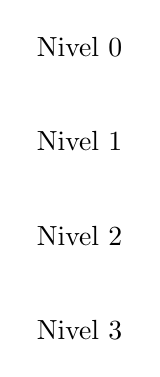
\begin{tikzpicture}[scale=1.2]
        \draw (0,0) node {Nivel 0};
        \draw (0,-1) node {Nivel 1};
        \draw (0,-2) node {Nivel 2};
        \draw (0,-3) node {Nivel 3};
        \end{tikzpicture}
    \end{tabular}
\end{center}
    \caption{Un árbol con raíz y sus niveles} \label{f6.1}
\end{figure}

Un vértice en un árbol con raíz se llama una \textit{hoja} si \index{hoja} pertenece al nivel $i$ ($i\ge 0$) y no es adyacente a ningún vértice del nivel $i+1$. Un vértice que no es una hoja es llamado \textit{interno}.  \index{vértice interno} La \textit{altura} de un árbol con raíz  \index{altura de un árbol con raíz} es el máximo valor de $k$ para el cual el nivel $k$ es no vacío. Luego el árbol de la Fig. \ref{f6.1} tiene seis hojas, cuatro vértices internos y su altura es tres.

Las dos propiedades que usamos en la sección \ref{5.5} para definir un árbol, ser un grafo conexo y sin ciclos, tienen consecuencias obvias cuando pensamos los vértices por niveles. Puesto que todo árbol es conexo entonces cada vértice pertenece a algún nivel. Más importante aún, puesto que un árbol no tiene ciclos  cada
vértice $v$ del nivel $i$ es adyacente a uno y solo uno $u$ del nivel $i-1$. A veces enfatizaremos esto diciendo que $u$ es el \textit{{padre}} de $v$ o que $v$ es un \textit{{hijo}} de $u$. Cada \index{padre de un vértice}  \index{hijo de un vértice} vértice, excepto el raíz, tiene un único padre, pero un vértice puede tener una cantidad arbitraria de hijos (incluso ninguno). Claramente, un vértice es una hoja si y solo si no tiene hijos.

En muchas aplicaciones ocurre que cada padre (vértice interno) tiene la misma cantidad de hijos. Cuando cada padre tiene $m$ hijos diremos que el árbol es \textit{$m$-ario}, en particular cuando $m=2$ diremos que el árbol es \textit{binario}  \index{árbol binario}  \index{árbol ternario} y cuando $m=3$ diremos que es \textit{ternario}.

\begin{teorema}\label{t6.1} La altura de un árbol con raíz $m$-ario con $l$ hojas es por lo menos $\log_ml$.
\end{teorema}
\begin{proof} Puesto que
$$
h \ge \log_ml \quad \Leftrightarrow \quad m^h \ge l
$$
es suficiente probar la afirmación equivalente: todo árbol con raíz $m$-ario de altura $h$ tiene a lo más $m^h$ hojas. La demostración es por inducción sobre $h$.

Claramente la afirmación es verdadera cuando $h=0$ puesto que en este caso el árbol es solo un vértice (la raíz) que es una hoja. Supongamos que la afirmación es verdadera cuando $0\le h \le h_0$ y sea $T$ un árbol con raíz $m$-ario de altura $h_0+1$. Si eliminamos la raíz y las aristas a las cuales pertenece obtenemos $m$ árboles $T_1,\ldots,T_m$ cuyas raíces son los vértices del nivel 1 de $T$. Cada $T_i$ es un árbol con raíz de altura $h_0$ o menos, luego por hipótesis inductiva tiene a lo más $m^{h_0}$ hojas. Pero las hojas de $T$ son precisamente las hojas de los árboles $T_1,\ldots,T_m$ y por consiguiente el número de hojas es a lo más $m \cdot m^{h_0}= m^{h_0+1}$.

Por el principio de inducción completa se sigue que la afirmación es verdadera para todo $h\ge 0$.
\end{proof}

Puesto que $\log_ml$ no es generalmente un número entero, el teorema anterior puede ser mejorado un poco. Por ejemplo si $m=3$ y $l=10$ la desigualdad
$$
h \ge \log_ml=2,0959\ldots
$$
implica que $h\ge 3$. En general podemos decir que
$$
h\ge\lceil \log_ml\rceil,
$$
donde $\lceil x \rceil$ denota el menor entero $z$ tal que $z\ge
x$.

Una aplicación frecuente del teorema \ref{t6.1} es en los  \index{árbol de decisión} \textit{árboles de decisión}. Cada vértice interno de un árbol de decisión representa una decisión y los posibles resultados de esa decisión son las aristas que unen ese vértice con los vértices del nivel siguiente. Los posibles  esultados finales del procedimiento son las hojas del árbol. Si el resultado de una decisión puede ser solo verdadero o falso entonces tenemos un árbol binario. A continuación daremos un ejemplo con un árbol ternario.

\begin{ejemplo} \label{monedafalsa}(El problema de la moneda falsa) Supongamos que tenemos una moneda genuina con la etiqueta $0$ y que tenemos otras $r$ monedas indistinguibles de $0$ por la apariencia excepto que tienen las etiquetas $1,2,\ldots,r$. Se sospecha que una moneda podría ser falsa, es decir o más liviana o más pesada. Probemos que son necesarias al menos $\lceil \log_3(2r+1)\rceil $ pesadas en una balanza para decidir que moneda (si hay alguna) es falsa y en ese caso ver si es más pesada o liviana. Mostremos un procedimiento que use exactamente este número de pesadas cuando $r=4$.
\end{ejemplo}
\begin{proof}[Solución] Hay $2r+1$ posibles resultados finales u hojas en el árbol de decisión: 
$$
B,1P,1L,\ldots,rP,rL;
$$
donde $B$ significa que todas las monedas son buenas, $iL$ significa que la moneda $i$ es más liviana y $iP$ que es más pesada. El árbol de decisión es ternario, puesto que hay tres posibles resultados de cada decisión (es decir de cada pesada entre un grupo de monedas y otro). Estos son:
\begin{alignat*}3
&<\quad & &:\quad& &\text{el grupo de la izquierda es más liviano}\\
&=\quad & &:\quad& &\text{los dos grupos pesan igual}\\
&>\quad & &:\quad& &\text{el grupo de la izquierda es más pesado.}
\end{alignat*}
Por consiguiente la altura del árbol de decisión es al menos $\lceil \log_3(2r+1)\rceil$.

Cuando $r=4$ entonces $\lceil \log_3(2r+1)\rceil=2$, y la solución con dos pesadas se gráfica en la Fig.\-\,\ref{f6.2}

\begin{figure}[ht]
    \begin{center}
    \begin{tikzpicture}[scale=1.2]
    {\renewcommand{\VertexShape}{rectangle}
        \Vertex[x=0.00, y=0, L ={\;$0,1 | 2,3$\;}]{0}
        \Vertex[x=-3, y=-1.5, L={$2|3$}]{1}
        \Vertex[x=0, y=-1.5, L={$0|4$}]{2}
        \Vertex[x=3, y=-1.5, L={\,$2|3$\,}]{3}
        \Vertex[x=-3.8, y=-3]{$3H$}
        \Vertex[x=-3, y=-3]{$1L$}
        \Vertex[x=-2.2, y=-3]{$2H$}
        \Vertex[x=-0.8, y=-3]{$4H$}
        \Vertex[x=0, y=-3]{$G$}
        \Vertex[x=0.8, y=-3]{$4L$}
        \Vertex[x=2.2, y=-3]{$2L$}
        \Vertex[x=3, y=-3]{$1H$}
        \Vertex[x=3.8, y=-3]{$3L$}
    }
    \SetVertexSimple[Shape=rectangle,FillColor=white,MinSize=8 pt]
    %\draw (0, 0) node {$\boxed{\text{Primera casa}}$};
    \Edges(0,1,0,2,0,3)
    \Edges(1,$3H$,1,$1L$,1,$2H$)
    \Edges(2,$4H$,2,$G$,2,$4L$)
    \Edges(3,$2L$,3,$1H$,3,$3L$)
    \end{tikzpicture}
    \end{center}
    \caption{Solución del problema de la moneda falsa cuando $r=4$}
    \label{f6.2}
\end{figure}

\end{proof}

\subsection*{$\S$ Ejercicios}
\begin{enumerate}
\item En la siguiente tabla $n_5(h)$ es el número de árboles con raíz no isomorfos que tienen $5$ vértices y altura $h$. (Dos árboles con raíz son isomorfos si hay un isomorfismo de grafos, sin considerar la raíz, que lleva la raíz de uno en la del otro.) Verificar la tabla construyendo los ejemplos para cada caso.
$$
\begin{matrix}
h: &1 &2 &3 &4 \\
n_5(h): &1 &4 & 3 &1
\end{matrix}
$$
\item Si se consideran los árboles comunes (sin raíz), ¿cuál es el número de árboles no isomorfos con $5$ vértices? Hacer una lista y controlar que la lista del ejercicio anterior sea completa.

\item Construir dos árboles con raíz no isomorfos ambos con $12$ vértices, $6$ hojas y altura $4$.    
    
\item Suponer que se organiza un campeonato de fútbol-$5$ donde participan $20$ equipos. El cam\-peo\-na\-to es por eliminación simple y no hay empates. Cons\-truir un esquema para el torneo basado en un árbol con raíz y pruebar que son necesarias al menos $5$ rondas. 

\item ¿Cuál es la cota inferior en el número de pesadas necesarias en el problema de la moneda falsa (ver el ejemplo \ref{monedafalsa}) cuando son seis monedas? Desarrollar un esquema que logre este número de pesadas.

\item Considerar la siguiente variante del problema de la moneda falsa. Hay ocho monedas y sabemos que hay exactamente una que es más liviana. Todas las demás son genuinas pero no hay ninguna moneda con la etiqueta $0$. Encontrar una cota inferior teórica del número de pesadas necesarias para detectar la moneda falsa y probar que este número puede ser alcanzado.
\end{enumerate}

\end{section}


\begin{section}{Árboles expandidos y el problema MST} \label{6.2}

\begin{definicion}
    Sea  $G=(V,E)$ es un grafo conexo y  $T$ es un subconjunto de $E$ tal que
    \begin{enumerate}[label=\textit{\alph*)}]
        \item  cada vértice de $G$ pertenece a una arista en $T$;
        \item  las aristas de $T$ forman un árbol.
    \end{enumerate}
    En este caso decimos que $T$ es un \textit{árbol expandido} para \index{árbol expandido} $G$.  
\end{definicion}
   Por ejemplo, un árbol expandido para el grafo de la Fig. \ref{f6.3} se indica con las líneas más gruesas.

Es fácil hacer ``crecer'' un árbol expandido: tome un vértice arbitrario $v$ del ``árbol parcial'' inicial y agregue aristas con un extremo en $v$ y el otro extremo que no pertenezca al árbol parcial inicial. El árbol expandido de la Fig. \ref{f6.3} puede construirse haciéndolo crecer desde el vértice $a$ y conectando los otros vértices en el orden $b$, $c$, $e$, $f$, $d$, $h$, $g$, usando las aristas $ab$, $ac$, $ae$, $cf$,  $fd$, $fh$, $hg$. En general, si hay $n$ vértices nosotros deberemos hacer $n-1$ pasos, después de los cuales tendremos $1+(n-1)=n$ vértices y $n-1$ aristas (el cual es el número correcto de acuerdo al teorema \ref{t5.5}).

\begin{figure}[ht]
    \begin{center}
        \begin{tikzpicture}[scale=1.2]
        \SetVertexSimple[Shape=circle,MinSize=5 pt,FillColor=white]
        \Vertex[x=0.00, y=0]{0}
        \Vertex[x=0.00, y=2.00]{1}
        \Vertex[x=1.90, y=0.62]{2}
        \Vertex[x=1.18, y=-1.62]{3}
        \Vertex[x=-1.18, y=-1.62]{4}
        \Vertex[x=-1.90, y=0.62]{5}
        \Edges(1,2,3,4,5,1)
        \Edges(5,0,c,2)
        \Edges(0,e,3)
        \Edges(0,c)
        \Vertex[x=0.59, y=0.19]{c}
        \Vertex[x=0.36, y=-0.49]{e}
        \tikzstyle{edge} = [draw,line width=2.5pt]
        \draw[edge] (5) -- (1) -- (2);
        \draw[edge] (1) -- (0) -- (e) -- (c) -- (e) -- (3) -- (4);
        \tikzstyle{edge} = [draw,line width=1pt]
        \draw[edge] (0) -- (c);
        \draw (0,2.3) node {$a$};
        \draw (-2.2, 0.62) node {$b$};
        \draw (2.2, 0.62) node {$e$};
        \draw (-0.2, -0.2) node {$c$};
        \draw (0.59, 0.5) node {$d$};
        \draw (0.66, -0.49) node {$f$};
        \draw (-1.48, -1.62) node {$g$};
        \draw (1.48, -1.62) node {$h$};
        \end{tikzpicture}
    \end{center}
    \caption{Un grafo y uno de sus árboles expandidos} \label{f6.3}
\end{figure}


Verifiquemos que el método siempre funciona: sea $S$ el conjunto de vértices del árbol parcial que se ha logrado en un paso intermedio, es decir que $S$ no es ni vacío ni todo $V$. Si no existe una arista que tenga un extremo en $S$ y el otro en el complemento $\overline{S}$, entonces no existe un camino entre $S$ y $\overline{S}$ y por lo tanto $G$ es disconexo, lo cual contradice las hipótesis. Por consiguiente siempre existe una arista disponible en cada etapa de la construcción.

Los árboles expandidos son útiles en muchos contextos. Por ejemplo, su\-pon\-ga\-mos que cierta cantidad de ciudades deben ser unidas de a pares por gasoductos de tal forma que quede una red de gasoductos conexa. Algunos pares de ciudades puede ser imposible unirlas por razones geográficas y cada posible conexión tiene asociada un costo de construcción. Formalmente, tenemos un grafo $G=(V,E)$ cuyos vértices son ciudades y sus aristas son las posibles conexiones. Además te\-ne\-mos una función $w$ de $E$ a $\mathbb N$ de tal forma que $w(e)$ representa el costo de cons\-truc\-ción de la arista $e$. Diremos que $G$ y $w$ es un \textit{grafo con pesos} y que $w$ es la \textit{función de pesos}. \index{grafo con pesos} \index{función de pesos}

En el problema del gasoducto lo que se pretende es construir una red conexa al mínimo costo. Un red de ese tipo corresponde a un árbol expandido $T$ para $G$ cuyo peso total 
$$
w(T) = \sum_{e \in T} w(e)
$$
es lo mas pequeño posible. Nos referiremos a este problema como el \textit{problema MST }(del inglés MST = minimum spanning tree = \index{MST}  \index{minimum spanning tree} árbol expandido mínimo) para el grafo con pesos $G$.  \index{árbol expandido mínimo}

Dado que los valores de $w$ son enteros positivos, claramente el problema MST debe tener solución, puesto que hay solo un número finito de árboles expandidos $T$ para $G$ y cada uno de ellos da un valor entero positivo $w(T)$. En otras palabras, existe un árbol expandido mínimo $T_0$ tal que 
$$
w(T_0) \le w(T)
$$
para todos los árboles expandidos $T$ de $G$. Sin embargo puede haber varios con la misma propiedad.

Un algoritmo simple para el problema MST se basa en aplicar la estrategia greedy al método explicado anteriormente. Específicamente: en cada paso se agrega la arista ``más barata'' que une un nuevo vértice al árbol parcial. (Si hay varias aristas con la misma propiedad se selecciona una de ellas.) Por ejemplo,
si en la Fig. \ref{f6.4} comenzamos con $u$, luego debemos agregar aristas en el orden $uv$, $ux$, $uy$, $yz$. Por otro lado, si comenzáramos por $y$, entonces agregamos las aristas en el orden $yz$, $yu$, $uv$, $ux$. 

\begin{figure}[ht]
    \begin{center}
    \begin{tikzpicture}[scale=1.2]
    \SetVertexSimple[Shape=circle,MinSize=5 pt,FillColor=white]
    \Vertex[x=0.00, y=2.00]{1}
    \Vertex[x=1.90, y=0.62]{2}
    \Vertex[x=1.18, y=-1.62]{3}
    \Vertex[x=-1.18, y=-1.62]{4}
    \Vertex[x=-1.90, y=0.62]{5}
    \Edges(1,2,3,4,5,1)
    \Edges(1,3,5,2,4,1)
    \tikzstyle{edge} = [draw,line width=2.5pt]
    \draw[edge] (1) -- (2) -- (1) -- (3) -- (1) -- (4) -- (5);
    \draw (0,2.3) node {$u$};
    \draw (-2.2, 0.62) node {$z$};
    \draw (2.2, 0.62) node {$v$};
    \draw (-1.48, -1.62) node {$y$};
    \draw (1.48, -1.62) node {$x$};
    \GraphInit[vstyle=Classic]
    \Edge[label=2](1)(2)
    \Edge[label=6](1)(5)
    \Edge[label=5](1)(4)
    \Edge[label=4](1)(3)
    \Edge[label=8](2)(5)
    \Edge[label=7](2)(4)
    \Edge[label=5](2)(3)
    \Edge[label=6](3)(5)
    \Edge[label=7](3)(4)
    \Edge[label=2](4)(5)
    \end{tikzpicture}
    \end{center}
    \caption{Un árbol expandido mínimo} \label{f6.4}
\end{figure}

El  algoritmo puede ser descripto informalmente en los siguientes pasos:
\begin{itemize}
\item Inicializar un árbol con un sólo vértice (elegido arbitrariamente).
\item Agrandar el árbol agregando una arista: entre las aristas que conectan al árbol con vértices que aún no están en el árbol, elegir una de peso mínimo.
\item Repetir el paso anterior hasta que todos los vértices estén en el árbol
\end{itemize}

Un primera impresión nos dice que sería bastante sorprendente que el algoritmo greedy funcione para el problema MST, especialmente cuando recordamos que el algoritmo greedy para el problema de coloración de vértices no siempre produce una coloración con el menor número posible de co\-lo\-res. Pero en el caso del problema MST se tiene más suerte.

\begin{teorema}\label{t6.2} Sea $G=(V,E)$ grafo conexo con función de pesos $w: E \to  \mathbb N$, y supongamos que $T$ es el árbol expandido para $G$ construido por el algoritmo greedy. Entonces 
$$
w(T) \le w(U) \nopagebreak
$$
para todo árbol expandido $U$ de $G$.
\end{teorema}
\begin{proof} Denotemos $e_1,e_2,\ldots,e_{n-1}$ las aristas de $T$ en el orden en que aplicamos el algoritmo greedy. Si $U=T$ el resultado es obviamente verdadero. Si $U\not=T$ entonces hay aristas de $T$ que no están en $U$ y supongamos que la primera es $e_k$. Denotemos $S$ el conjunto de vértices en el árbol parcial que se construye por el greedy justo antes de agregar $e_k$ y sea $e_k=xy$ donde $x$ está en $S$ e $y$ no está
en $S$. Puesto que $U$ es un árbol expandido existe un camino de $x$ a $y$ y si uno viaja a través de este camino encontrará una arista $e^*$ con un vértice en $S$ y el otro no. Ahora bien, cuando $e_k$ es seleccionada para $T$ en el algoritmo greedy, $e^*$ es también candidata a ser seleccionada, pero no lo es. Por consiguiente debemos tener que $w(e^*) \ge w(e)$. Si $e^*$ aparece en $T$, entonces por el razonamiento anterior es una arista que viene después (en el orden dado) de $e_k$.

El resultado de remover $e^*$ de $U$ y reemplazarla por $e_1$ es un árbol expandido $U_1$, para el cual
$$
w(U_1) = w(U) -w(e^*)+w(e_k) \le w(U).
$$
Más aún, la primera arista de $T$ que no está en $U_1$ aparece después de $e_k$ en el orden dado. En consecuencia podemos repetir el procedimiento obteniendo una sucesión de árboles expandidos $U_1,U_2,\ldots,$ con la propiedad que cada uno tiene una secuencia inicial de aristas en común con las aristas de $T$ más
larga que el anterior y además $w(U_i) \ge w(U_{i+1})$. El proceso termina cuando obtenemos un árbol expandido $U_r$ igual a $T$ y tenemos
$$
w(T)=w(U_r) \le w(U_{r-1}) \le \cdots \le w(U_1) \le w(U),
$$
como queríamos demostrar.
\end{proof}

En forma más detallada, el algoritmo puede ser implementado con el siguiente pseudocódigo:

\vskip .5cm

\begin{minipage}{400pt}
\noindent \textsc{Algoritmo de Prim}
\vskip .2cm
\begin{small}
\begin{verbatim}
# pre: G grafo con vértices 1,...,n y pesos w(i,j)
#      (w(i,j) = infinito si ij no es arista de G)
# post: devuelve F un MST de G
S = [1] # lista de vértices utilizados en el MST (comienza con 1)
Q = [2,...,n]  # lista de vértices aún no utilizados en el MST
L = [[2,1,p2],...,[n,1,pn]]]  # con pi = w(i,1)
# se irá modificando L de tal forma que si Q = [u1,...,ur], 
# L  = [[u1,v1,p1],...,[ur,vr,pr]] donde 
# vi = vértice en S adyacente a ui tal que w(ui,vi) es mínimo, 
# pi = w(ui,vi)
F = grafo con vértices 1,...,n y sin aristas.
while Q != []:
    uk = vértice en Q tal que pk = w(uk,vk) es mínimo
    F.append(arista uk,vk)
    Q = Q - {uk}
    S.append(uk)
    L = L - {[uk,vk,pk]}
    for [ui,vi,pi] in L:
        if w(ui,uk) < pi:
            vi = uk
            pi = w(ui,uk)
    # el for modifica L
\end{verbatim}
\end{small}
\end{minipage}

\vskip .5cm

Notemos que terminamos el proceso no cuando $S$ contiene todos los vértices, si no cuando, de manera equivalente, su complemento $Q$ queda vacío.   Existe una forma de ir viendo el progreso del algoritmo por medio de una tabla de tres columnas.
$$
\begin{matrix}
\text{I} &\text{II} & \text{III} \\
x & y & w(xy)\\
 .& .&. \\
. & .&. \\
. &. & .
\end{matrix}
$$

La Columna I lista los vértices que no están en $S$, que es el conjunto de vértices ya conectados al árbol parcial. Para cada $x$ en la Columna I la correspondiente entrada $y$ en la Columna II es un vértice en $S$ tal que la arista $xy$ es una de las aristas más baratas que unen el vértice $x$ con alguno de $S$. La  Columna III contiene el valor $w(xy)$.

En el $i$-ésimo paso de la construcción tenemos que $|S|=i$ y hay $n-i$ vértices en la Columna I. Tenemos entonces que seleccionar una de las entradas más pequeñas de la Columna III, digamos $w(x_0y_0)$, y esto conlleva $n-i-1$ comparaciones. Ahora debemos actualizar la tabla debido a que agregamos $x_0$ a $S$ por medio
de la arista $x_0y_0$. Primero debemos borrar la fila cuya primera posición tiene a $x_0$. Después en cada fila debemos verificar si la entrada correspondiente a la Columna II puede ser reemplazada por $x_0$ o no. Es decir para la fila $"x\quad y \quad w(xy)"$ debemos verificar si $xx_0$ es arista y si lo fuera y además $w(xx_0) < w(xy)$, entonces debemos reemplazar $y$ por $x_0$. Esto agrega otras $n-i-1$ comparaciones. El número total de comparaciones requeridas es
$$
\sum_{i=1}^{n-1} 2(n-i-1) = (n-1)(n-2).
$$
Esto nos dice que para encontrar un MST de un grafo deben hacerse alrededor de $n^2$ operaciones.

\subsection*{$\S$ Ejercicios}
\begin{enumerate}
    \item Encontrar árboles expandidos para el cubo Fig. \ref{f5.12} y para el grafo de Petersen.

    \item Muestrar esquemáticamente todos los árboles expandidos del grafo completo $K_4$ (hay $16$).    

    \item Usar el algoritmo greedy para encontrar un MST del grafo representado en la Fig. \ref{f6.5}. ¿Es en este caso el MST único?
    \begin{figure}[ht]
    \begin{center}
    \begin{tikzpicture}[scale=1.8]
    %\SetVertexSimple[Shape=circle,MinSize=5 pt,FillColor=white]
    \Vertex[x=0.00, y=0.00, L = $a$]{1}
    \Vertex[x=1.5, y=1, L =$b$]{2}
    \Vertex[x=1.5, y=-0, L=$c$]{3}
    \Vertex[x=1.5, y=-1, L=$d$]{4}
    \Vertex[x=3, y=1, L =$e$]{5}
    \Vertex[x=3, y=-0, L=$f$]{6}
    \Vertex[x=3, y=-1, L=$g$]{7}
    \Vertex[x=4.5, y=1, L =$h$]{8}
    \Vertex[x=4.5, y=-0, L=$i$]{9}
    \Vertex[x=4.5, y=-1, L=$j$]{10}
    \Vertex[x=6, y=-0, L=$k$]{11}
    \Edge[label=2](1)(2)
    \Edge[label=8](1)(3)
    \Edge[label=1](1)(4)
    \Edge[label=6](2)(3)
    \Edge[label=7](3)(4)
    \Edge[label=1](2)(5)
    \Edge[label=1](3)(6)
    \Edge[label=9](4)(7)
    \Edge[label=2](5)(8)
    \Edge[label=6](6)(9)
    \Edge[label=1](7)(10)
    \Edge[label=9](8)(11)
    \Edge[label=2](9)(11)
    \Edge[label=4](10)(11)
    \Edge[label=5](3)(5)
    \Edge[label=1](3)(6)
    \Edge[label=2](3)(7)
    \Edge[label=3](5)(6)
    \Edge[label=4](6)(7)
    \Edge[label=9](5)(9)
    \Edge[label=3](7)(9)
    \Edge[label=7](8)(9)
    \Edge[label=1](9)(10)
    \end{tikzpicture}
    \end{center}
    \caption{Encontrar el MST} \label{f6.5}
\end{figure}

\item Sea $G$ un grafo con pesos cuyos vértices son $x,a,b,c,d,e,f$ y cuyas aristas y pesos vienen dados por la siguiente tabla:

\begin{align*}
xa &&xb &&xc &&xd &&xe &&xf &&ab &&bc &&cd &&de &&ef &&fa \\
6  &&3  &&2  &&4  &&3  &&7  &&6  &&2  &&3  &&1  &&8  &&6.
\end{align*}

Encontrar todos los árboles expandidos mínimos para $G$.

\item Suponer que $T$ es un árbol expandido mínimo en un grafo con pesos $K$ y sea $e^*$ una arista de $K$ que no es de $T$. Sea $e$ una arista de $T$ perteneciente al único camino en $T$ que une los vértices de $e^*$. Probar que $w(e) \le w(e^*)$. 

\item Escribir un ``programa'' para el algoritmo greedy basado en el
método ta\-bu\-lar mostrado más arriba.
\end{enumerate}

\section{Ejercicios}
\begin{enumerate}
\item Sea $T$ un árbol con raíz $m$-ario con $n$ vértices, $l$ hojas e $i$ vértices internos. Probar que
$$ n=mi+1$$
y encontrar la ecuación de $l$ en términos de $m$ y $n$.

\item Para cada uno de los seis diferentes árboles (sin raíz) con seis vértices (ver el ejercicio \ref{ejercicios5.5}\ref{ejercicio5.5.1}, encontrar el número de elecciones esencialmente diferentes que se pueden hacer de un vértice para designarlo como raíz. En base a esto calcular el número de árboles con raíz diferentes que tengan seis vértices.

\item Probar que el número de árboles expandidos mínimos diferentes en $K_5$ es 125 (no trate de listarlos).

\item Denotar los vértices del grafo completo $K_n$ con $1, 2, \ldots,n$, y para cada árbol expandido $T$ de $K_n$ definir el \textit{símbolo de Prüfer} $(p_1,p_2,\ldots,p_{n-2})$ de la \index{símbolo de Prüfer} siguiente manera: el símbolo de Prüfer de un árbol con dos vértices es $0$, el símbolo de Prüfer de un árbol $T$ con $n$ vértices es $(j,q_1,\ldots,q_{n-3})$ donde 
\begin{enumerate}
\item  Si $i$ es el primer vértice de $T$ (en el orden dado) que tiene valencia uno, entonces $j$ es el único vértice adyacente a $i$.
\item $(q_1,\ldots,q_{n-3})$ es el símbolo de Prüfer del árbol que se obtiene a partir de $T$ eliminando la arista $ij$.
\end{enumerate}
Probar que la construcción del símbolo de Prüfer define una biyección desde el conjunto de árboles expandidos de $K_n$ al conjunto de $(n-2)$-uplas ordenadas del conjunto $\{1,2,\ldots,n\}$. Deducir de lo anterior que $K_n$ tiene $n^{n-2}$ árboles expandidos.

 \item Suponer que tenemos cuatro monedas y sabemos que una de ellas puede ser falsa (más liviana o más pesada) . Probar que encontrar la moneda falsa (si existe) requiere teóricamente al menos dos pesadas, pero que este número no es posible lograrlo. (En este problema no se da un moneda verdadera.)
\end{enumerate}

\end{section}


\appendix

\part{Ap\'endices} 

\setcounter{chapter}{0}
\renewcommand{\thechapter}{\Alph{chapter}}


\chapter[Permutaciones]{Permutaciones}


\begin{section}{Permutaciones}
Recordemos  que una \textit{permutación} de un conjunto finito no vacío $X$ es una biyección de $X$ en $X$. (Frecuentemente tomamos $X$ como $ [[1,n]]=\{1,2,\ldots,n\}$.) Por ejemplo una permutación típica de $[[1,5]]$ es la función $\alpha$ definida por las ecuación
$$
\alpha(1)=2,\quad \alpha(2)=4,\quad \alpha(3)=5,\quad
\alpha(4)=1,\quad \alpha(5)=3.
$$

Denotemos el conjunto de todas las permutaciones de $[[1,n]]$ con $S_n$. Por ejemplo, $S_3$ contiene las $3!=6$ permutaciones siguientes:
$$
\begin{matrix} 1&2&3 \\ \downarrow&\downarrow&\downarrow\\1 &2 &
3\end{matrix}\qquad
\begin{matrix} 1&2&3 \\ \downarrow&\downarrow&\downarrow\\1 &3 &2 \end{matrix}\qquad
\begin{matrix} 1&2&3 \\ \downarrow&\downarrow&\downarrow\\2 & 1&3 \end{matrix}
\qquad
\begin{matrix} 1&2&3 \\ \downarrow&\downarrow&\downarrow\\2 & 3&1
\end{matrix}\qquad
\begin{matrix} 1&2&3 \\
\downarrow&\downarrow&\downarrow\\3 &1 &2 \end{matrix}\qquad
\begin{matrix} 1&2&3 \\ \downarrow&\downarrow&\downarrow\\3 &2 &1
\end{matrix}
$$


En la práctica, usualmente asignamos alguna interpretación concreta a un elemento de $S_n$. Como vimos en la sección \ref{permutaciones}, podemos usar la interpretación ``selecciones ordenadas sin repetición''  \index{selección ordenada sin repetición} donde, en este caso seleccionamos los elementos de $\{1,2,3,\ldots,n\}$ en algún orden hasta que no queda ninguno. Una interpretación relacionada es que una permutación efectúa un \textit{reacomodamiento} de $\{1,2,3,\ldots,n\}$; por ejemplo, la permutación $\alpha$ vista más arriba  efectúa el reacomodamiento de $12\,345$, en $24\,513$, así:
$$
\begin{matrix} 1&2&3&4&5 \\
\downarrow&\downarrow&\downarrow&\downarrow&\downarrow\\2 &4 &5 &1
& 3
\end{matrix}
$$
En algunas circunstancias es conveniente mirar una permutación y el correspondiente reacomodamiento como la misma cosa, pero esto puede traer dificultades si debemos considerar sucesivos reacomodamientos. Es importante tener en cuenta que 
$$
\textit{una permutación es una función con ciertas características.}
$$

Cuando las permutaciones son tratadas como funciones es claro como deben combinarse. Consideremos $\alpha$ la permutación de $[[1,5]]$ antes mencionada, y sea $\beta$ la permutación de $[[1,5]]$ dada por 
$$
\beta(1)=3,\quad \beta(2)=5,\quad \beta(3)=1,\quad
\beta(4)=4,\quad \beta(5)=2.
$$
La función compuesta $\beta\alpha$ es la permutación definida por $(\beta\alpha)(i)= \beta(\alpha(i))$ ($1\le i\le 5$), esto es 
$$
\beta\alpha(1)=5,\quad \beta\alpha(2)=4,\quad
\beta\alpha(3)=2,\quad \beta(4)\alpha=3,\quad \beta\alpha(5)=1.
$$
(Recordemos que, como siempre, $\beta\alpha$ significa ``primero $\alpha$, entonces $\beta$''.) En términos de reacomodamientos tenemos
$$\begin{aligned}
\alpha\quad&\quad\begin{matrix} 1&2&3&4&5 \\
\downarrow&\downarrow&\downarrow&\downarrow&\downarrow\\2 &4 &5 &1
& 3
\end{matrix} \\
\beta \quad&\quad \begin{matrix} 1&2&3&4&5 \\
\downarrow&\downarrow&\downarrow&\downarrow&\downarrow\\5 &4 &2 &3
& 1
\end{matrix}
 \end{aligned}
$$



Existen cuatro características de la composición de permutaciones de gran importancia, y están listadas en el próximo teorema.

\begin{teorema}\label{tA3} Las siguientes propiedades valen en el conjunto $S_n$ de todas las permutaciones de $\{1,2,3,...,n\}$.
\begin{enumerate}[label=\textit{\alph*)}]
\item  Si $\pi$ y $\sigma$ pertenecen a $S_n$, entonces $\pi\sigma$ también.
\item  Para cualesquiera permutaciones $\pi$, $\sigma$, $\tau$ en $S_n$,
$$
(\pi\sigma)\tau=\pi(\sigma\tau).$$
\item  La función identidad, denotada por $\operatorname{id}$ y definida por $\operatorname{id}(r) =r$ para todo $r$ en $\mathbb N_n$, es una permutación y para cualquier $\sigma$ en $S_n$,
tenemos
$$
\operatorname{id}\sigma=\sigma\operatorname{id}=\sigma.$$
\item  Para toda permutación $\pi$ en $S_n$ hay una permutación inversa $\pi^{-1}$ en $S_n$ tal que
$$
\pi\pi^{-1} = \pi^{-1}\pi = \operatorname{id}.
$$
\end{enumerate}
\end{teorema}
\begin{proof} Todas las afirmaciones se deducen de propiedades conocidas de funciones en general y funciones biyectivas en particular. Por otro lado, es fácil convencerse de la validez de las mismas mirando las permutaciones como reacomodamiento de elementos. 
\end{proof}


Es conveniente tener una notación más compacta para las permutaciones. Consideremos otra vez la permutación $\alpha$ de $\{1,2,3,4,5\}$, y notemos en particular que
$$
\alpha(1)=2,\qquad \alpha(2)=4,\qquad \alpha(4)=1.
$$
Así $\alpha$ lleva $1$ a $2$, $2$ a $4$ y $4$ a $1$, y por esta razón decimos que los símbolos $1, 2, 4$ forma un \textit{ciclo } (de longitud $3$). Del mismo modo, los símbolos $3$ y $5$ forman un ciclo de longitud $2$, y
escribimos:
$$
\alpha=(1\,2\,4)(3\,5).
$$
Esta es la \textit{notación cíclica} para $\alpha$. Cualquier \index{notación cíclica} permutación $\pi$ puede ser escrita cíclicamente de la siguiente manera:
\begin{itemize}
\item comencemos con algún símbolo (digamos el $1$) y veamos el efecto de $\pi$ sobre él y sus sucesores hasta que alcancemos el $1$
nuevamente;
\item elijamos un símbolo que todavía no haya aparecido y construyamos el ciclo que se deriva de él; 
\item repitamos el procedimiento hasta que se terminen los símbolos.
\end{itemize}
Por ejemplo, la permutación $\beta$ definida antes tiene la notación cíclica
$$
\beta=(1\,3)(2\,5)(4),
$$
donde observamos que el símbolo $4$ forma un ciclo ``degenerado'' por sí solo, puesto que $\beta(4)=4$. En algunas ocasiones podemos omitir estos ciclos de longitud 1 cuando escribimos una permutación en notación cíclica, puesto que corresponden a símbolos que no son afectados por la permutación. Sin embargo, usualmente es útil \textit{no} adoptar esta convención hasta que uno se familiariza con la notación.


Aunque la representación de una permutación en notación cíclica es esencialmente única, hay dos manera obvias en las que podemos cambiar la notación sin alterar la permutación. Primero, cada ciclo puede empezar en cualquiera de sus símbolos; por ejemplo $(7\,8\,2\,1\,3)$ y $(1\,2\,7\,8\,2)$ describen el mismo ciclo. Segundo, el orden de los ciclos no es importante; por ejemplo $(1\,2\,4) (3\,5)$ y $(3\,5) (1\,2\,4)$ denotan la misma permutación. Pero las características importantes son el número de ciclos, la longitud del ciclo, y la disposición de los símbolos dentro de los ciclos, y éstas están determinadas de manera única. Por eso, la rotación cíclica nos dice bastantes cosas útiles sobre una permutación.

\begin{ejemplo}\label{cartas} Cartas numeradas del $1$ al $12$ son distribuidas en una mesa en la manera en que se muestra en la parte izquierda de la tabla que sigue. Luego las cartas son levantadas  por filas (de izquierda a derecha y de arriba hacia abajo) y se redistribuyen con el mismo arreglo, pero por columnas, no por filas (de arriba hacia abajo y de izquierda a derecha), apareciendo como se muestra en la parte derecha de la tabla.
$$
\begin{matrix} 1& 2& 3\\
4 &5 &6 \\
7 &8 & 9\\
10 &11 & 12 \end{matrix}\qquad \qquad\qquad
\begin{matrix}1 &5 &9 \\
2 &6 &10 \\
3& 7& 11\\
4&8 & 12 \end{matrix}
$$
¿Cuántas veces debe repetirse este procedimiento hasta que las cortas aparezcan dispuestas como estaban inicialmente?
\end{ejemplo}
\begin{proof}[Solución] Sea $\pi$ la permutación que efectúa el reordenamiento; esto es $\pi(i) =j$ si la carta $j$ aparece en la posición previamente ocupada por la carta $i$. Trabajando con la notación cíclica para $\pi$ encontramos que
$$
\pi=(1)(2\,\,5\,\,6\,\,10\,\,4)(3\,\,9\,\,11\,\,8\,\,7)(12).
$$
Los ciclos degenerados $(1)$ y $(12)$ indican que las cartas 1 y 12 nunca cambian de posición. Las otros ciclos tienen longitud 5, así que cuando el proceso se haya realizado 5 veces las cartas
reaparecerán en sus posiciones originales. Otra forma de expresar el resultado es decir que $\pi^5= \operatorname{id}$, donde $\pi^5$ representa las cinco repeticiones de la permutación $\pi$.
\end{proof}
\end{section}


\subsection*{$\S$ Ejercicios}
\begin{enumerate}
\item Escribir en notación cíclica la permutación que realiza el siguiente reordenamiento:
$$
\begin{matrix} 1&2&3&4&5&6&7&8&9 \\
\downarrow&\downarrow&\downarrow&\downarrow&
\downarrow&\downarrow&\downarrow&\downarrow&\downarrow
\\ 3&5 &7 &8 &4 &6 &1 &2 &9
\end{matrix}
$$

\item Sean $\sigma$ y $\tau$ las permutaciones de $[[1,8]]$ cuyas representaciones en la notación cíclica son
$$
\sigma= (1\,2\,3)(4\,5\,6)(7\,8),\qquad
\tau=(1\,3\,5\,7)(2\,6)(4)(8).
$$
Escribir en notación cíclica $\sigma\tau$, $\tau\sigma$, $\sigma^2$, $\sigma^{-1}$, $\tau^{-1}$. 

\item Resolver el problema presentado en el ejemplo \ref{cartas} cuando hay $20$ cartas acomodadas en $5$ filas de $4$.

\item Probar que hay exactamente tres elementos de $S_4$ que tienen dos ciclos de longitud $2$, escritos en la notación cíclica. 

\item Sea $K$ el subconjunto de $S_4$ que contiene la identidad y las tres permutaciones descritas en el ejercicio previo. Escribir la ``tabla de multiplicación'' para $K$, interpretando la multiplicación como la composición de permutaciones.

\item Calcular en número total de permutaciones $\sigma$ de $\mathbb [[1,6]]$ que satisfacen $\sigma^2=\text{id}$ y $\sigma\not=\text{id}$.
\item Sean $\alpha$ y $\beta$ permutaciones de $[[1,9]]$ cuyas representaciones en la notación cíclica son:
$$
\alpha= (1237)(49)(58)(6),\qquad \beta=(135)(246)(789).
$$
Escribir en notación cíclica $\alpha\beta$, $\beta\alpha$, $\alpha^2$, $\beta^2$, $\alpha^{-1}$, $\beta^{-1}$.

\item Sea $X_1=\{0,1\}$, y para $i\ge 2$ definamos $X_i$ como el conjunto de subconjuntos de $X_{i-1}$. Encontrar el valor más pequeño para el cual $|X_i|>10^{100}$.

\item Por cada entero $i$ en el rango $1 \le i \le n-1$ definimos $\tau_i$ como la permutación de $[[1,n]]$ que intercambia $i$ e $i+1$ y no afecta los otros elementos. Explícitamente 
$$
\tau_i = (1)(2)\cdots(i-1)(i\ i+1)(i+2)\cdots(n).
$$
Probar que toda permutación de $[[1,n]]$ puede ser expresada en términos de $\tau_1,\tau_2,\ldots,\tau_{n-1}$. 

\item Una permutación de $[[1,n]]$ que tenga solo un ciclo (necesariamente de longitud $n$) es llamada \textit{cíclica}  \index{permutación cíclica}. Probar que hay $(n-1)!$ permutaciones cíclicas de $[[1,n]]$.

\item Un mazo de $52$ cartas es dividido en dos partes iguales y luego se alternan las cartas de una y otra parte. Es decir si la numeración original era $1,2,3,\ldots,54$, el nuevo orden es $1,27,2,28,\ldots$ ¿Cuántas veces se debe repetir este procedimiento para obtener de nuevo el mazo original? 
\end{enumerate}


\chapter[El principio del tamiz]{El principio del tamiz} \label{ape.principio_del_tamiz}

\begin{section}{El principio del tamiz}\label{Ap1.2}
El principio más básico del conteo (proposición \ref{principiodeadicion}) dice que $|A \cup B|$ es la suma de $|A|$ y $|B|$, cuando $A$ y $B$ son conjuntos disjuntos. Si $A$ y $B$ no son disjuntos, cuando sumamos $|A|$ y $|B|$ estamos contando $A \cap B$ dos veces. Entonces, para obtener la respuesta correcta debemos restar $|A \cap B|$:
$$
|A \cup B| = |A|+|B| - |A \cap B|.
$$

Un método similar puede aplicarse a tres conjuntos. Cuando sumamos $|A|$, $|B|$ y $|C|$, los elementos de $A \cap B$, $B \cap C$, y $C \cap A$ son contados dos veces (si no están en los tres conjuntos). Para corregir esto, restamos $|A \cap B|$, $|B \cap C|$ y $|C \cap A|$. Pero ahora los elementos de $A \cap B \cap C$, contados originalmente tres veces, han sido descontados tres veces. Luego, para conseguir la respuesta correcta, debemos sumar $|A \cap B \cap C|$. Así
$$
|A \cup B\cup C|= \alpha_1-\alpha_2+\alpha_3,
$$ 
donde
$$\gathered
\alpha_1=|A|+|B|+|C|,\qquad \alpha_2= |A \cap B|+|B \cap C|+|C \cap A|, \\
\alpha_3 = |A \cap B \cap C|.
\endgathered
$$

Este resultado es un caso simple de lo que suele ser llamado, por razones obvias, el principio de inclusión y exclusión. También \index{principio de inclusion y exclusion} se lo llama el \textit{principio del tamiz}.  \index{principio del tamiz}

\begin{teorema}\label{tA1.2} Si $A_1,A_2,\ldots,A_n$ son conjuntos finitos, entonces 
$$ |A_1 \cup A_2 \cup \ldots \cup A_n|= \alpha_1-\alpha_2+\alpha_3 + \cdots +(-1)^n\alpha_n, $$ donde $\alpha_i$ es la suma de los cardinales de las intersecciones de los conjuntos tomados de a $i$ por vez ($1\le i \le n$).
\end{teorema}
\begin{proof} Debemos demostrar que cada elemento $x$ de la unión hace una contribución neta de 1 al miembro de la derecha. Supongamos que $x$ pertenece a $k$ de los conjuntos $A_1, A_z,\ldots,A_n$. Entonces $x$  contribuye con $k$ en la suma $\alpha_1=|A_1|+\cdots+|A_n|$. En la suma $\alpha_2$, $x$ contribuye 1 en $|A_i \cap A_j|$ cuando $A_i$ y $A_j$ están entre los $k$ conjuntos que contienen a $x$. Existen $\binom{k}{2}$ de esos pares, por lo tanto $\binom{k}{2}$ es la contribución de $x$ a $\alpha_2$. En general la contribución de $x$ a $\alpha_i$ ($1 \le i \le n$) es $\binom{k}{i}$. Por lo tanto el total con que contribuye $x$ al lado derecho de la igualdad es 
$$
\binom{k}{1} -\binom{k}{2} + \cdots + (-1)^{k-1} \binom{k}{k},
$$
porque los términos con $i > k$ dan cero.

Por el teorema del binomio aplicado a $(1-1)^k=0$, se deduce que la expresión de arriba  es igual a
$\binom{k}{0}$, que vale $1$.
\end{proof}

Un corolario simple del teorema \ref{tA1.2} es a menudo más útil en la práctica. Supongamos que $X$ es un conjuntos finito y $A_1,A_2,\ldots,A_n$ son subconjuntos de $X$ (cuya unión no necesariamente es igual a $X$). Si $|X| = N$, entonces el número de elementos de $X$ que no están en ninguno de esos subconjuntos es
$$\begin{aligned}
|X-(A_1 \cup A_2 \cup \ldots \cup A_n)|&=
|X|-|A_1 \cup A_2 \cup \ldots \cup A_n| \\
&= N- \alpha_1 + \alpha_2 - \cdots + (-1)^n\alpha_n.
\end{aligned}
$$

\begin{ejemplo*} Hay $73$ estudiantes en el primer año de la Escuela de Artes de la universidad. De ellos, $52$ saben tocar el piano, $25$ el violín y $20$ la flauta; $17$ pueden tocar tanto el piano como el violín, $12$ el piano y la flauta; pero solo Juan Rictero puede tocar los tres instrumentos ¿Cuántos alumnos no saben tocar ninguno de esos instrumentos?
\end{ejemplo*}
\begin{proof}[Solución] Con $V$, $P$ y $F$ denotaremos los conjuntos de estudiantes que saben tocar el violín, el piano y la flauta respectivamente. Usando la información dada tenemos que $$
\begin{aligned}
\alpha_1&= |P| + |V| + |F|= 52+25+20=97 \\
\alpha_2&= |P\cap V| + |V\cap F| + |P\cap F|=17+7+12=36 \\
\alpha_3&= |P\cap V\cap F|= 1.
\end{aligned}
$$
Por consiguiente, el número de estudiantes que o pertenecen a ninguno de los tres conjuntos $P$, $V$ y $F$ es
$$
73-97+36-1=11.
$$
\end{proof}

\begin{ejemplo*} Una secretaria ineficiente tiene $n$ cartas distintas y $n$ sobres con direcciones ¿De cuántas maneras puede ella arreglárselas para meter cada carta en un sobre equivocado? (Esto es comúnmente llamado el \textit{problema del desarreglo} del cual hay varias formulaciones pintorescas.) 
\end{ejemplo*}


\begin{proof}[Solución] Podemos considerar cada carta y su correspondiente sobre  como si estuvieran etiquetadas con un entero $i$ en el rango $1 \le i \le n$. El acto de poner las cartas en los sobres puede describirse como una permutación $\pi$  de $\mathbb N_n$: $\pi(i)=j$ si la carta $i$ va en el sobre $j$. Necesitamos saber  el número de \textit{desarreglos}, esto es, las permutaciones $\pi$ tales que
$\pi(i)\not=i$ para todo $i$ en $\mathbb N_n$.

Denotemos $A_i$ ($1 \le i \le n$) el subconjunto de $S_n$ (el conjunto de permutaciones de $\mathbb N_n$) que contiene aquellos $\pi$ tales que $\pi(i)=i$. Diremos que los elementos de $A_i$ \textit{fijan} $i$. Por el principio del tamiz, el número de desarreglos es 
$$
d_n= n! -\alpha_1+\alpha_2 - \cdots +(-1)^n\alpha_n,
$$
donde $\alpha_r$ es la suma de los cardinales de las intersecciones de los $A_i$ tomando r por vez. En otras palabras, $\alpha_r$ es el número de permutaciones que fijan $r$ símbolos dados, tomando todas las maneras de elegir los $r$ símbolos. Ahora hay $\binom{n}{r} $ maneras de elegir $r$ símbolos, y el número de  permutaciones que los fijan es solo el número de permutaciones de los restantes $n-r$ símbolos, que es $(n-r)!$  Por lo tanto
$$
\alpha_r = \binom{n}{r} \cdot (n-r)! = \frac{n!}{r!},\qquad d_n=
n!\left(1-\frac{1}{1!} + \frac{1}{2!}-\cdots
+(-1)^n\frac{1}{n!}\right). \nopagebreak$$
\end{proof}

\subsection*{$\S$ Ejercicios}
\begin{enumerate}
\item En una clase de $67$ estudiantes de matemática, $47$ leen francés, $35$ leen alemán y $23$ leen ambos lenguajes ¿Cuántos estudiantes no lee ninguno de los dos lenguajes? Si además $20$ leen ruso, de los
cuales $12$ también leen francés, $11$ leen alemán y $5$ leen los tres lenguajes, ¿cuántos estudiantes no leen ninguno de los tres lenguajes?

\item Encontrar el número de formas de ordenar las letras A, E, M, O, U, Y en una secuencia de tal forma que las palabras ME e YOU no aparezcan. 

\item
Calcular el número $d_4$ de desarreglos de $\{1,2,3,4\}$ y escriba, en la notación cíclica, las permutaciones relevantes.

\item Usar el principio de inducción para probar que la fórmula para $d_n$ satisface la recursión
$$
d_1=0, \quad d_2=1,\quad d_n= (n-1)(d_{n-1}+d_{n-2}) \ (n\ge 3).
$$

\item Probar que el número de desarreglos de $\{1,2,\ldots,n\}$ en el cual un objeto dado (digamos el $1$) está en un $2$-ciclo es $(n-1)d_{n-2}$. Utilizar esto para dar una prueba directa de la fórmula recursiva del ejercicio anterior.
\end{enumerate}

\end{section}


\chapter[La función de Euler]{La función de Euler}\label{ape.funcion_de_euler}

 \begin{section}{La función de Euler} \label{A2.1 }

 En esta sección probaremos un útil e importante teorema, usando sólo  los conceptos de conteo más básicos.

 El teorema se refiere a las  propiedades de divisibilidad de los enteros. Recordemos que dos enteros $x$ e
 $y$ son \textit{coprimos} si el $\mcd(x,y) = 1$. Por cada $n \ge 1$ sea  $\phi(n)$ el número de  enteros $x$ en el rango $1 \le x \le n$ tal que $x$ y $n$ son coprimos.  Podemos  calcular los primeros valores de $\phi(n)$ haciendo una tabla (tabla  \ref{tablaA2.1.1}).

La función es llamada \textit{función de Euler}, debido a Leonhard Euler  \index{Euler, Leonhard} ($1\,707-1\,783$). Cuando $n$ es primo, digamos $n=p$, cada uno de los enteros $1,2,\ldots,p-1$ es coprimo con $p$, entonces tenemos 
$$
\phi(p)=p-1,\qquad\text{ $p$ primo.}
$$

\begin{table}[h]
\begin{center}
       \begin{tabular}{r|r|r}
              $n$&  Coprimos a $n$ \,&\,$\phi(n)$\\
             \hline
              $1$&$1$&$1$ \\
              $2$&$1$&$1$ \\
              $3$&$1$,$2$&$2$ \\
              $4$&$1$,$3$&$2$ \\
              $5$&$1$,$2$,$3$,$4$&$4$ \\
              $6$&$1$,$5$&$2$ \\
              $7$&$1$,$2$,$3$,$4$,$5$,$6$&$6$ \\
              $8$&$1$,$3$,$5$,$7$&$4$
       \end{tabular}
\end{center}
 \caption{Primeros valores de $\phi(n)$} \label{tablaA2.1.1}
\end{table}

Nuestra tarea ahora es probar un resultado respecto a la suma de los valores $\phi(d)$, donde los $d$ son todos los divisores de un número positivo $n$ dado. Por ejemplo, cuando $n=12$, lo divisores $d$ son $1$, $2$, $3$, $4$, $5$, $6$ y $12$, podemos ver que
\begin{align*}
&\quad\phi(1)+\phi(2)+\phi(3)+\phi(4)+\phi(6)+\phi(12)\\
&= 1 +1+2+2+2+4 \\
&=12.
\end{align*}

Debemos demostrar que la suma es siempre igual al entero $n$ dado.

\begin{teorema}\label{tA2.1b} Para cualquier $n$ entero positivo,
$$
\sum_{d|n} \phi(d)=n.
$$
\end{teorema}
\begin{proof} Sea $S$ el conjunto de pares de enteros $(d,f)$ que
satisfacen
$$
d|n, \qquad 1\le f \le d, \qquad \mcd(f,d)=1.
$$


\begin{table}
\begin{tabular}{rr|rrrrrrrrrrrrr|c}
  &$f$ &$1$  &$2$ &$3$ &$4$ &$5$  &$6$ &$7$ &$8$ &$9$ &$10$ &$11$ &$12$ & &$\phi(d)$\\
$d$ &  &   &  &  &  &   &  &  &  &  &   &   &   & &   \\\hline
$1$ &  &$12$ &  &  &  &   &  &  &  &  &   &   &   & &$1$  \\
$2$ &  &$6$  &  &  &  &   &  &  &  &  &   &   &   & &$1$  \\
$3$ &  &$4$  &$8$ &  &  &   &  &  &  &  &   &   &   & &$2$  \\
$4$ &  &$3$  &  &$9$ &  &   &  &  &  &  &   &   &   & &$2$  \\
$6$ &  &$2$  &  &  &  &$10$ &  &  &  &  &   &   &   & &$2$  \\
$12$&  &$1$  &  &  &  &$5$  &  &$7$ &  &  &   &$11$ &   & &$4$  \\
  &  &   &  &  &  &   &  &  &  &  &   &   &   & &$12$
\end{tabular}
\caption{} \label{tablaA2.1.2}
\end{table}


La tabla \ref{tablaA2.1.2} muestra $S$ cuando $n=12$; la ``marca'' que indica que $(d,f)$ pertenece a $S$ es un número cuya importancia explicaremos en seguida. Por lo general, el número de ``marcas'' en la fila $d$ es el número de $f$'s en el rango $1\le f\le d$ que satisfacen que el $\mcd(d,f)=1$; esto es $\phi(d)$. Por lo tanto, contando $S$ por el método de las filas obtenemos
$$
|S| = \sum_{d|n} \phi(d).
$$
Para demostrar que $|S|=n$ debemos construir una biyección $\beta$ de $S$ en $\mathbb N_n$. Dado un par $(d,f)$ en $S$, definimos
$$
\beta(d,f) = f n/d.
$$
En la tabla, $\beta(d,f)$ es la ``marca'' en la fila $d$ y la columna $f$. Como $d| n$, el valor de $\beta$, es un entero y como $1\le f\le d$, entonces $\beta(d,f)$ pertenece a $\mathbb N_n$.

Para probar que $\beta$ es una inyección observemos que
$$
\beta(d,f) = \beta(d',f') \quad \Rightarrow \quad fn/d = f'n/d'
\quad \Rightarrow \quad fd'=f'd.
$$
Pero $f$ y $d$ son coprimos, así como también lo son $f'$ y $d'$, así que podemos concluir que $d=d'$ y $f=f'$.

Para demostrar que $\beta$ es una suryección, supongamos que nos dan un $x$ que pertenece a $\mathbb N_n$. Sea $g_x$ el mcd de $x$ y $n$, y sea
$$
d_x = n/g_x, \qquad f_x = x /g_x.
$$
Puesto que $g_x$ es un divisor de $x$ y $n$, entonces $d_x$ y $f_x$ son enteros, y como $g_x$ es el mcd, $d_x$ y $f_x$ son coprimos. Ahora
$$
\beta(d_x,f_x) = f_x n/d_x = x,
$$
y por lo tanto $\beta$ es suryectiva.  Luego $\beta$ es biyectiva y $|S|=n$, como queríamos demostrar.
\end{proof}

\subsection*{$\S$ Ejercicios}
\begin{enumerate}
\item Encontrar los valores de $\phi(19),\quad \phi(20),\quad \phi(21)$.

\item Probar que si $x$ y $n$ son coprimos, entonces lo son $n-x$ y $n$. Deducir que $\phi(n)$ es par para todo $n \ge 3$.

\item Probar que, si $p$ es un primo y $m$ es un entero positivo, entonces un entero $x$ en el rango $1 \le x \le p^m$ \textit{no} es coprimo a $p^m$ si y solo si es un múltiplo de $p$. Deducir que $\phi(p^m) = p^m - p^{m-1}$.

\item Encontrar un contraejemplo que confirme que es falsa la conjetura $\phi(ab)= \phi(a)\phi(b)$, para enteros cualesquiera $a$ y $b$. Trate de modificar la conjetura de tal forma que no pueda
encontrar un contraejemplo. 

\item Probar que para cualesquiera enteros positivos $n$ y $m$ se cumple: 
$$
\phi(n^m) =n^{m-1}\phi(n).
$$

\item Calcular $\phi(1\,000)$ y $\phi(1\,001)$.
\end{enumerate}

\end{section}



\begin{section}{Una aplicación aritmética del principio del tamiz}\label{Ap2.2} 
Por cientos de años los matemáticos han estudiado problemas sobre números primos y la fac\-to\-ri\-za\-ción de los enteros. Nuestra breve discusión sobre estos temas en los primeros capítulos debería haber convencido al lector de que estos problemas son difíciles, porque los primos mismos se encuentran irregularmente distribuidos, y porque no hay una forma directa de encontrar la factorización en primos de un entero dado. De todos modos, si se nos da la factorización en primos de un entero, es relativamente fácil responder ciertas preguntas sobre sus propiedades aritméticas. Supongamos, por ejemplo que queremos listar todos los divisores de un entero $n$ y sabemos que la factorización de $n$ es
$$
n=p_1^{e_1}p_2^{e_2}\cdots p_r^{e_r}.
$$
Entonces un entero $d$ es divisor de $n$ si y solo si no tiene divisores primos distintos de los de $n$, y ningún primo divide más veces a $d$ que a $n$. Visto así, los divisores son precisamente los enteros que pueden escribirse de la forma
$$
d=p_1^{f_1}p_2^{f_2}\cdots p_r^{f_r},
$$
donde cada $f_i$ ($1\le i \le r$) satisface $0\le f_i \le e_i$. Por ejemplo dado que $60= 2^2 \cdot 3 \cdot 5$ podemos listar rápidamente todos los divisores de 60.

Un problema similar es encontrar el número de enteros $x$ en el rango $1 \le x \le n$ que son coprimos con $n$. En la sección \ref{A2.1 } denotamos este número con $\phi(n)$, el valor de la función $\phi$ de Euler en $n$. Ahora demostraremos que si la factorización en primos de $n$ es conocida, entonces $\phi(n)$ puede ser calculado por el principio del tamiz.

\begin{ejemplo*}¿Cuál es el valor de $\phi(60)$? En otras palabras, ¿cuántos enteros $x$ en el rango $1 \le x \le 60$ satisfacen $\operatorname{mcd}(x,60)=1$?
\end{ejemplo*}
\begin{proof}[Solución] Sabemos que $60 =2^2 \cdot 3 \cdot 5$, así que podemos contar el números de enteros $x$ en el rango $1 \le x \le 60$ que no son divisibles por $2$, $3$ o $5$. Con $A(2)$ denotemos el subconjunto de $\mathbb N_{60}$ que contiene los enteros que \textit{son} divisibles por $2$, con $A(2,3)$ aquellos que \textit{son} divisibles por $2$ y $3$, y así sucesivamente, entonces tenemos 
$$\begin{aligned}
\phi(60)&=60-|A(2) \cup A(3) \cup A(5)| \\
&= 60-|A(2) + A(3) + A(5)| \\
&\qquad+(|A(2,3) + |A(2,5)| + |A(3,5)|)-|A(2,3,5)|,
\end{aligned}
$$
por el principio del tamiz. Ahora $|A(2)|$ es el número de múltiplos de $2$ en $\mathbb N_{60}$ que es $60 /2 = 30$. Del mismo modo $|A(2,3)|$ es el número de múltiplos de $2 \cdot 3$, que es $60 /(2\cdot 3) = 10$, y así siguiendo, por lo tanto
$$
\phi(60) = 60 -(30+20+10)+(10+6+4)-2=16.
$$
\end{proof}

El mismo método puede ser usado para dar una fórmula explícita para $\phi(n)$ en el caso general.

\begin{teorema}\label{tA2.2} Sea $n \ge 2$ un entero cuya factorización es $n=p_1^{e_1}p_2^{e_2}\ldots p_r^{e_r}$. Entonces $$
\phi(n)=n\left(1-\frac{1}{p_1}\right)\left(1-\frac{1}{p_2}\right)\cdots\left(1-\frac{1}{p_r}\right).
$$
\end{teorema}
\begin{proof} Denotemos $A_j$ el subconjunto de $\mathbb N_n$ que contiene los múltiplos de $p_j$ ($1\le j \le r$). Entonces 
$$
\begin{aligned}
\phi(n) &= n- |A_1 \cup A_2 \cup \cdots \cup A_r| \\
       &= n -\alpha_1+ \alpha_2- \cdots +(-1)^r\alpha_r
\end{aligned}
$$
donde $\alpha_i$ es la suma de los cardinales de las intersecciones de los conjuntos tomados de a $i$. Una intersección típica como
$$
A_{j_1}\cup A_{j_2}\cup \cdots \cup A_{j_i}
$$
contiene los múltiplos de $P= p_{j_1}\cdot p_{j_2}\cdots p_{j_i}$ en $\mathbb N_n$, y estos son los números
$$
P,2P,3P,\ldots,\left(\frac{n}{p}\right)P.
$$
Luego la cardinalidad de una intersección típica es $n/P$, y $\alpha_i$ es la suma de términos como
$$
\frac{n}{P}= n\left(\frac{1}{p_{j_1}}\right)\left(\frac{1}{p_{j_2}}\right)\cdots \left(\frac{1}{p_{j_i}}\right).
$$
Se sigue que
\begin{multline*}
    \phi(n) = n - n\left(\frac{1}{p_1} + \frac{1}{p_2} + \cdots +\frac{1}{p_r}\right) +n\left(\frac{1}{p_1p_2} + \frac{1}{p_1p_3}+\cdots\right) + \cdots \\
    \cdots + (-1)^r \left(\frac{1}{p_1p_2 \cdots p_r}\right) =\\
    =n\left(1-\frac{1}{p_1}\right)\left(1-\frac{1}{p_2}\right)\cdots\left(1-\frac{1}{p_r}\right).
\end{multline*}


\end{proof}

\end{section}


\chapter[Grafos planares]{Grafos planares}\label{ape.grafos_planares}

\begin{section}{Grafos planares}\label{Ap4.1} 

Usualmente el diagrama de un grafo se realiza en el plano por la comodidad que esto representa. Esto no significa que todo grafos sea lo que se denomina un {\em grafo planar}. ¿Qué es un grafo \index{grafo planar} planar? Es un grafo tal que \textit{existe} un diagrama del grafo en el plano tal que no hay ningún cruce de
aristas. Por ejemplo, el grafo $K_3$ es claramente planar Fig. \ref{fA4.1}-(a).  Claro que podríamos dibujar a $K_3$ como en la Fig. \ref{fA4.1}-(b) y no parecería planar.

\begin{figure}[ht]
    \begin{center}
        \begin{tabular}{cccc}
            &
            \begin{tikzpicture}[scale=1]
            \SetVertexSimple[Shape=circle,FillColor=white,MinSize=8 pt]
            \Vertex[x=0.00, y=0]{a}
            \Vertex[x=-0.5, y=1]{b}
            \Vertex[x=2., y=0]{c}
            \Edges(a,b,c,a)
            \end{tikzpicture}
            &
            \qquad
            & 
            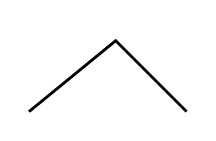
\begin{tikzpicture}[scale=1]
            \draw[-,line width=1pt] (0,0) -- (1.1,0.9) -- (2,0);
            \SetVertexSimple[Shape=circle,FillColor=white,MinSize=8 pt]
            \Vertex[x=0.00, y=0]{a}
            \Vertex[x=-0.5, y=1]{b}
            \Vertex[x=2., y=0]{c}
            \Edges(a,b,c)
            \tikzstyle{vertex}=[circle,minimum size=5pt]
            \node[vertex] (v0) at (1.1,0.9) {};
            \Edges(a,v0,c)
            
            %\node[vertex] (v1) at (-0.5,1) {b};
            %\node[vertex] (v2) at (2,0) {c};
            \end{tikzpicture} 
            \\
            &(a)&&(b)
        \end{tabular}
    \end{center}
    \caption{Dibujos de $K_3$} \label{fA4.1}
\end{figure}

Pero la definición es que un grafo es planar si se {\em puede} dibujar en el plano sin cruces de aristas, no si {\em todo} dibujo no tiene cruces. (Si la definición fuera así, ningún grafo seria planar, pues siempre se puede dibujar cualquier grafo con cruces). Otro ejemplo, ya visto, $K_4$ puede ser dibujado como en la Fig. \ref{fA4.2}-(a) y no parece planar, pero dibujado como en la Fig. \ref{fA4.2}-(b) muestra que $K_4$ es planar.

\begin{figure}[ht]
    \begin{center}
        \begin{tabular}{cccc}
            &
            \begin{tikzpicture}[scale=1]
            \SetVertexSimple[Shape=circle,FillColor=white,MinSize=8 pt]
            \Vertex[x=0.00, y=0]{a}
            \Vertex[x=2, y=0]{b}
            \Vertex[x=2, y=2]{c}
            \Vertex[x=0, y=2]{d}
            \Edges(a,b,c,d,a)
            \Edges(a,c)
            \Edges(b,d)
            \end{tikzpicture}
            &
            \qquad
            & 
            \begin{tikzpicture}[scale=1]
                    \SetVertexSimple[Shape=circle,FillColor=white,MinSize=8 pt]
            \Vertex[x=0.00, y=0]{a}
            \Vertex[x=1.15, y=2]{b}
            \Vertex[x=2.31, y=0]{c}
            \Vertex[x=1.15, y=0.8]{d}
            \Edges(a,b,c,d,a)
            \Edges(a,c)
            \Edges(b,d)
            \end{tikzpicture} 
            \\
            &(a)&&(b)
        \end{tabular}
    \end{center}
    \caption{Dibujos de $K_4$} \label{fA4.2}
\end{figure}

En vista de estos ejemplos, una pregunta es ¿existen grafos no planares? Por ejemplo si dibujáramos $K_{16}$ parecería imposible que fuera planar, dada la gran cantidad de cortes, pero ¿cómo podemos estar seguros?

Observemos primero que si $G$ es planar y $H$ es subgrafo de $G$, entonces $H$ es planar, pues, si podemos dibujar a $G$ en el plano sin cortes de aristas, entonces $H$ que esta ``metido'' en $G$, también puede ser así dibujado. Así, como ya vimos que $K_4$ es planar, sabemos que todo subgrafo de él es planar; es decir, todo grafo con cuatro o menos vértices es planar. Esta observación tiene consecuencias en la otra dirección también: si encontramos un grafo $H$ que {\em no} sea planar, entonces todo grafo $G$ que lo tenga como subgrafo deberá necesariamente ser no planar, pues si $G$ fuera planar, $H$ también lo seria. Así, si  queremos probar que $K_{16}$ no es planar, bastará con encontrar algún subgrafo mas sencillo de el que no lo sea. De hecho, probaremos que $K_5$ no es planar, con lo cual todos los grafos $K_n$, con $n\ge 5$ son no planares.

En lo que sigue veremos un arma poderosa para probar que un grafo es no planar: la llamada ``fórmula de Euler''.  \index{fórmula de Euler} Supongamos que un grafo {\em sí} es planar. Escojamos un diagrama
de él en el plano (puede haber muchos, escojamos uno). Este diagrama divide al plano en varias regiones. Por ejemplo, si $G$ esta representado por el dibujo de la Fig. \ref{fA4.3}, entonces se obtienen regiones que numeraremos como en la Fig. \ref{fA4.4} ($1$ es la región ``exterior'' a todo el grafo).

\begin{figure}[h]
    \begin{center}
        \begin{tikzpicture}[scale=0.7]
        \SetVertexSimple[Shape=circle,FillColor=white,MinSize=8 pt]
        \Vertex[x=0.00, y=0]{0}
        \Vertex[x=0.5, y=2]{1}
        \Vertex[x=0.8, y=-2]{2}
        \Vertex[x=1.5, y=-0.2]{3}
        \Vertex[x=1.8, y=-2.2]{4}
        \Vertex[x=3.5, y=1.9]{5}
        \Vertex[x=3, y=0.1]{6}
        \Vertex[x=3.7, y=-1.7]{7}
        \Vertex[x=4, y=-0.1]{8}
        \Vertex[x=6, y=0.3]{9}
        \Vertex[x=5.5, y=1.8]{10}
        \Vertex[x=6, y=-2.2]{11}
        \Vertex[x=6.8, y=2]{12}
        \Vertex[x=7, y=-1.8]{13}
        \Vertex[x=7.5, y=0.8]{14}
        \Vertex[x=8.5, y=1.8]{15}
        \Vertex[x=9, y=-1]{16}
        \Edges(0,1,3,4,2,0)
        \Edges(1,5,6,7,4,7,8,5,9,8,9,7,11,9,5,10,12,14,15,16,13,11)
        \end{tikzpicture} 
    \end{center}
\caption{Un grafo planar} \label{fA4.3}
\end{figure}

En realidad, también podríamos considerar a la región formada por las regiones $3$ y $4$ juntas, o $2$, $5$ y $6$ juntas, etc. Pero nuestra preocupación estará centrada en una de estas regiones ``simples'', a las cuales llamaremos {\em caras}.  \index{caras de un grafo planar}

\begin{figure}[h]
    \begin{center}
    \begin{tikzpicture}[scale=0.7]
    \SetVertexSimple[Shape=circle,FillColor=white,MinSize=8 pt]
    \Vertex[x=0.00, y=0]{0}
    \Vertex[x=0.5, y=2]{1}
    \Vertex[x=0.8, y=-2]{2}
    \Vertex[x=1.5, y=-0.2]{3}
    \Vertex[x=1.8, y=-2.2]{4}
    \Vertex[x=3.5, y=1.9]{5}
    \Vertex[x=3, y=0.1]{6}
    \Vertex[x=3.7, y=-1.7]{7}
    \Vertex[x=4, y=-0.1]{8}
    \Vertex[x=6, y=0.3]{9}
    \Vertex[x=5.5, y=1.8]{10}
    \Vertex[x=6, y=-2.2]{11}
    \Vertex[x=6.8, y=2]{12}
    \Vertex[x=7, y=-1.8]{13}
    \Vertex[x=7.5, y=0.8]{14}
    \Vertex[x=8.5, y=1.8]{15}
    \Vertex[x=9, y=-1]{16}
    \Edges(0,1,3,4,2,0)
    \Edges(1,5,6,7,4,7,8,5,9,8,9,7,11,9,5,10,12,14,15,16,13,11)
    \draw (-2, 1) node {1};
    \draw (3.5, 0) node {2};
    \draw (4.3, 0.8) node {3};
    \draw (4.3, -0.7) node {4};
    \draw (2.2, 0) node {5};
    \draw (0.8, 0) node {6};
    \draw (5.4, -1.2) node {7};
    \draw (7.2, -0.5) node {8};
    \end{tikzpicture} 
    \end{center}
    \caption{Regiones de un grafo planar} \label{fA4.4}
\end{figure}


Observemos que no podemos hablar propiamente de las caras del grafo (aunque a veces lo haremos así) pues ellas son en realidad dependientes del diagrama, no del grafo. Sin embargo, algo puede decirse acerca de ellas:

\begin{teorema}\label{tA4.1} (Fórmula de Euler) Sea $G$ un grafo conexo, con $v$ vértices, y $e$ aristas. Supongamos que en algún diagrama planar de $G$, existen $f$ caras. Entonces, $v-e+f=2$.
\end{teorema}

Antes de ver la prueba, observemos que, puesto que $v$ y $e$ dependen de $G$ y no del diagrama, la fórmula de Euler dice que no importa como dibujemos a $G$ en el plano (siempre y cuando esto sea posible), entonces siempre obtendremos $e-v+2$ caras. Por lo tanto, el \textit{número} de caras es algo independiente del
diagrama, y podemos hablar del ``número de caras de un grafo planar''. Otra observación es que en el número de caras estamos contando la cara infinita, es decir, la exterior a todo el grafo. Finalmente, observemos que se pide que $G$ sea conexo. La fórmula debe ser alterada en caso contrario.

\begin{proof}[Demostración del teorema \ref{tA4.1}] Supongamos que la fórmula de Euler no sea cierta. Es decir, supongamos que existen grafos planares para los cuales la fórmula no es válida. Tomemos, de todos estos contraejemplos, alguno con $e$ tan chico como sea posible, y llamemos $G$ a ese grafo. Observemos que $G$ debe tener por lo menos un ciclo, pues si fuera acíclico, como es conexo, sería un árbol. Ahora bien, en un árbol, $e=v-1$. Además, por ser acíclico, no hay caras, salvo la cara infinita, es decir, $f$ seria 1. Pero entonces $v-e+f=v-(v-1)+1=v-v+1+1=2$ y $G$ no sería un contraejemplo. Así pues, $G$ tiene al menos un ciclo. Sea $xy$ alguna arista perteneciente a algún ciclo, y consideremos $H=G-xy$. Como $xy$ pertenece a algún ciclo, es una arista que separa dos caras en $G$. Esas dos caras ahora son una sola en $H$. 
Ver Fig. \ref{fA4.5}.

\begin{figure}[ht]
    \begin{center}
    \begin{tabular}{cccc}
        &
        \begin{tikzpicture}[scale=0.7]
        \SetVertexSimple[Shape=circle,FillColor=white,MinSize=8 pt]
        \Vertex[x=0.00, y=0]{0}
        \Vertex[x=0.5, y=-1]{1}
        \Vertex[x=-0.5, y=-2]{2}
        \Vertex[x=0, y=-3]{3}
        \Vertex[x=2, y=-4]{4}
        \Vertex[x=3.5, y=-3]{5}
        \Vertex[x=3.5, y=-2]{6}
        \draw (3., -2.1) node {$y$};
        \Vertex[x=2, y=-1]{7}
        \draw (2, -1.5) node {$x$};
        \Vertex[x=1.8, y=0.2]{8}
        \Vertex[x=3, y=0]{9}
        \Vertex[x=5, y=-0.2]{10}
        \Vertex[x=4.5, y=-2.7]{11}
        \Edges(0,1,2,3,4,5,6)
        \Edges(6,7)
        \Edges(7,8,0)
        \Edges(1,7)
        \Edges(8,9,10,11,5)
        \draw (1.5, -2.5) node {$A$};
        \draw (3.5, -1) node {$B$};
        \end{tikzpicture}
        &
        \qquad
        & 
        \begin{tikzpicture}[scale=0.7]
        \SetVertexSimple[Shape=circle,FillColor=white,MinSize=8 pt]
        \Vertex[x=0.00, y=0]{0}
        \Vertex[x=0.5, y=-1]{1}
        \Vertex[x=-0.5, y=-2]{2}
        \Vertex[x=0, y=-3]{3}
        \Vertex[x=2, y=-4]{4}
        \Vertex[x=3.5, y=-3]{5}
        \Vertex[x=3.5, y=-2]{6}
        \draw (3., -2.1) node {$y$};
        \Vertex[x=2, y=-1]{7}
        \draw (2, -1.5) node {$x$};
        \Vertex[x=1.8, y=0.2]{8}
        \Vertex[x=3, y=0]{9}
        \Vertex[x=5, y=-0.2]{10}
        \Vertex[x=4.5, y=-2.7]{11}
        \Edges(0,1,2,3,4,5,6)
        \Edges(7,8,0)
        \Edges(1,7)
        \Edges(8,9,10,11,5)
        \end{tikzpicture} 
    \end{tabular}
\end{center}
    \caption{Eliminar una arista} \label{fA4.5}
\end{figure}
Así, si $f_H,e_H$ y $v_H$ denotan el número de caras, aristas y vértices de $H$ respectivamente, te\-ne\-mos que $f_H=f-1$. Además, como borramos una arista, $e_H=e-1$, y como el número de vértices no cambia, $v_H=v$.

Pero, $e_H=e-1$ es menor que $e$, y $G$ era un contraejemplo con un número tan chico como fuera posible de aristas, por lo tanto, $H$ no es un contraejemplo, es decir, $v_H-e_H+f_H=2$. Reemplazando, obtenemos:
$$
v-e+f=v_H-(e_H+1)+f_H+1=v_H-e_H-1+f_H+1=v_H-e_H+f_H=2,
$$
lo cual dice que $G$ no es un contraejemplo, absurdo.
\end{proof}

La fórmula de Euler es una herramienta muy poderosa en la teoría de grafos planares. Para empezar, permite probar que un grafo planar no puede tener muchas aristas, en relación a sus vértices 
\begin{corolario}\label{cA4.1} Sea $G$ un grafo planar con al menos $3$ vértices. Entonces, $e\le 3v-6$, donde $e$ es el número de aristas y $v$ el número de vértices de $G$.
\end{corolario} \begin{proof} Consideremos las caras de $G$. Si es una cara distinta de la cara infinita, es porque viene de un ciclo. Ahora bien, todo ciclo debe tener por lo menos $3$ aristas, así que podemos concluir que hay por lo menos $3$ aristas en el borde de esa cara. Si, en cambio, es la cara infinita y el grafo tiene más de tres aristas entonces ``toca'' $3$ o más aristas. Si el grafo tiene menos de $3$ aristas (y ningún ciclo), es uno de los de la Fig. \ref{fA4.6}.  Como estamos suponiendo que hay al menos $3$ vértices, en realidad solo hay que considerar el último caso, y ese tiene $e=2$, $v=3$, y $2\le 3 \cdot 3-6$.

    \begin{figure}[ht]
        \begin{center}
        \begin{tabular}{cccc}
            &
            \begin{tikzpicture}[scale=0.7]
            \SetVertexSimple[Shape=circle,FillColor=white,MinSize=8 pt]
            \Vertex[x=0.00, y=0]{0}
            \Vertex[x=2, y=0]{1}
            \Edges(0,1)
            \end{tikzpicture}
            &
            \qquad\qquad
            & 
            \begin{tikzpicture}[scale=0.7]
            \SetVertexSimple[Shape=circle,FillColor=white,MinSize=8 pt]
            \Vertex[x=0.00, y=0]{0}
            \Vertex[x=2, y=0]{1}
            \Vertex[x=4, y=0]{2}
            \Edges(0,1,2)
            \end{tikzpicture} 
        \end{tabular}
    \end{center}
        \caption{Grafos acíclicos con menos de 3 aristas} \label{fA4.6}
    \end{figure}
    
Así pues, podemos suponer que en nuestro grafo, todas las caras tienen al menos $3$ aristas en su borde. Es decir:
$$
\begin{aligned}
3\le &\,\text{ Número de aristas en el borde de cara }1 \\
3\le &\,\text{ Número de aristas en el borde de cara }2\\
&\vdots \\
3\le &\,\text{ Número de aristas en el borde de cara }f.
\end{aligned}
$$
Si sumamos estas desigualdades, del lado izquierdo obtendremos $3f$. En el lado derecho, cada arista puede, o bordear dos caras, o bordear una. Pero ciertamente, no puede haber aristas que sean borde de $3$ caras. Así, si sumamos en el lado izquierdo, la suma nos dará menor o igual a $2e$. Por lo tanto, $3f\le 2e$. Tomando la fórmula de Euler y multiplicándola por $3$, obtenemos: $3v-3e+3f=6$. Usando ahora $3f\le 2e$, tenemos
$$
6=3v-3e+3f\le 3v-3e+2e=3v-e,$$ es decir, $e\le 3v-6$.
\end{proof}

Este corolario nos permite probar inmediatamente la no planaridad de un número significativo de grafos. Por ejemplo, recordemos que queríamos ver que $K_5$ era no planar. Esto lo obtenemos en forma directa, pues $K_5$ tiene $5$ vértices y $10$ aristas, por lo tanto, si fuera planar debiéramos tener que $10\le 3\cdot  -6=15-6=9$, lo cual no es cierto.
\end{section}

\begin{section}{El problema del agua-luz-gas}\label{Ap4.2} Este es un conocido problema de escuela primaria: existen tres casas, y tres centrales: la del agua, la de la luz y la del gas. Trazar las cañerías desde las centrales a las casas sin que se crucen. Una solución (pero haciendo trampa) es mandar las tres cañerías a una casa, y de ella sacarlas las tres a la otra, y de ella las tres a la otra:

    \tikzstyle{startstop} = [rectangle, rounded corners, minimum width=3cm, minimum height=1cm,text centered, draw=black, fill=gray!30]
    \tikzstyle{servicio} = [rectangle, rounded corners, minimum width=1cm, minimum height=1cm,text centered, draw=black, fill=gray!30]
 
\begin{figure}[ht]
    \begin{center}
        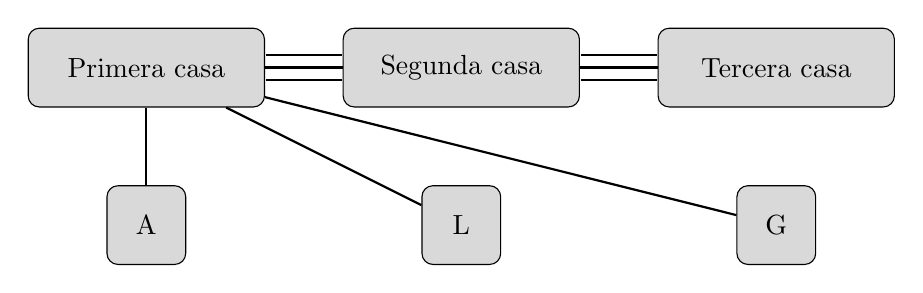
\begin{tikzpicture}[node distance=2cm,scale=0.8]
            \node (casa1) [startstop] {Primera casa};
            \node (casa2) [startstop, xshift=4cm] {Segunda casa};
            \node (casa3) [startstop, xshift=8cm] {Tercera casa};
            \node (A) [servicio, below of=casa1] {A};
            \node (L) [servicio, below of=casa2] {L};
            \node (G) [servicio, below of=casa3] {G};
            \draw [thick,-,>=stealth] (A) -- (casa1);
            \draw [thick,-,>=stealth] (L) -- (casa1);
            \draw [thick,-,>=stealth] (G) -- (casa1);
            \draw [thick,-,>=stealth] (casa1) -- (casa2);
            \draw [thick,-,>=stealth] (1.9,0.2) -- (3.1,0.2);
            \draw [thick,-,>=stealth] (1.9,-0.2) -- (3.1,-0.2); 
            \draw [thick,-,>=stealth] (casa2) -- (casa3);
            \draw [thick,-,>=stealth] (6.9,0.2) -- (8.1,0.2);
            \draw [thick,-,>=stealth] (6.9,-0.2) -- (8.1,-0.2); 
        \end{tikzpicture}
    \end{center}
    \caption{Una solución tramposa} \label{fA4.7}
\end{figure}

En realidad, no permitiremos el uso de intermediarios, es decir el problema será llevar directamente la cañería desde cada central a cada casa. En el lenguaje de la teoría de grafos, consiste en representar, en el plano, al grafo $K_{3,3}$ Fig. \ref{fA4.8}.

\begin{figure}[ht]
    \begin{center}
        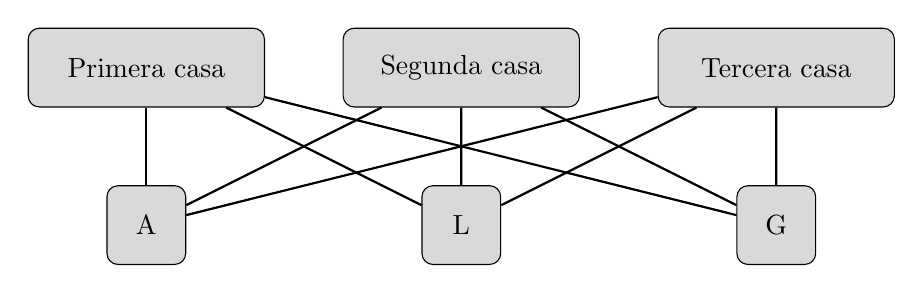
\begin{tikzpicture}[node distance=2cm,scale=0.8]
            \node (casa1) [startstop] {Primera casa};
            \node (casa2) [startstop, xshift=4cm] {Segunda casa};
            \node (casa3) [startstop, xshift=8cm] {Tercera casa};
            \node (A) [servicio, below of=casa1] {A};
            \node (L) [servicio, below of=casa2] {L};
            \node (G) [servicio, below of=casa3] {G};
            \draw [thick,-,>=stealth] (A) -- (casa1);
            \draw [thick,-,>=stealth] (L) -- (casa1);
            \draw [thick,-,>=stealth] (G) -- (casa1);
            \draw [thick,-,>=stealth] (A) -- (casa2);
            \draw [thick,-,>=stealth] (L) -- (casa2);
            \draw [thick,-,>=stealth] (G) -- (casa2);
            \draw [thick,-,>=stealth] (A) -- (casa3);
            \draw [thick,-,>=stealth] (L) -- (casa3);
            \draw [thick,-,>=stealth] (G) -- (casa3);
        \end{tikzpicture}
    \end{center}
    \caption{Luz-agua-gas es $K_{3,3}$} \label{fA4.8}
\end{figure}

La pregunta es entonces si $K_{3,3}$ es planar o no. Veamos si podemos usar esta fórmula que probamos recién: $K_{3,3}$ tiene $9$ aristas, y $6$ vértices. Desafortunadamente, $3 \cdot 6-6=18-6=12$ es ciertamente mayor que $9$, así que solo sabemos que quizás es planar. Pero, observemos que $K_{3,3}$, por ser bipartito, no tiene ningún triángulo como subgrafo. Así pues, deduciremos la no planaridad de $K_{3,3}$ del si\-guien\-te

\begin{corolario}\label{cA4.2} Si $G$ es un grafo planar con por lo menos $3$ vértices y que no tiene ningún triángulo como subgrafo, entonces $e\le 2v-4$.
\end{corolario}
\begin{proof} Es similar a la demostración del corolario \ref{cA4.1}, pero como no hay triángulos, todo ciclo tiene por lo menos $4$ aristas, es decir, cada cara esta bordeada por al menos $4$ aristas. Las únicas
excepciones con al menos $3$ vértices son los de la fig. \ref{fA4.9}

\begin{figure}[ht]
    \begin{center}
    \begin{tabular}{cccccc}
    &
    \begin{tikzpicture}[scale=0.5]
    \SetVertexSimple[Shape=circle,FillColor=white,MinSize=8 pt]
    \Vertex[x=0.00, y=0]{0}
    \Vertex[x=2, y=0]{1}
    \Vertex[x=4, y=0]{2}
    \Edges(0,1,2)
    \end{tikzpicture}
    &
    \qquad
    & 
    \begin{tikzpicture}[scale=0.5]
    \SetVertexSimple[Shape=circle,FillColor=white,MinSize=8 pt]
    \Vertex[x=0.00, y=0]{0}
    \Vertex[x=2, y=0]{1}
    \Vertex[x=4, y=0]{2}
    \Vertex[x=6, y=0]{3}
    \Edges(0,1,2,3)
    \end{tikzpicture} 
    &
    \qquad
    &
    \begin{tikzpicture}[scale=0.5]
    \SetVertexSimple[Shape=circle,FillColor=white,MinSize=8 pt]
    \Vertex[x=0.00, y=0]{0}
    \Vertex[x=0, y=1.3]{1}
    \Vertex[x=-1, y=-1]{2}
    \Vertex[x=1, y=-1]{3}
    \Edges(0,1,0,2,0,3)
    \end{tikzpicture} 
    \end{tabular}
\end{center}
    \caption{Grafos acíclicos con menos de $4$ aristas y al menos $3$
    vértices} \label{fA4.9}
\end{figure}

En el primer caso, $e=2$, $v=3$ y $2 \cdot 3-4=6-4=2$. En el segundo y terceros, $e=3$, $v=4$ y $2 \cdot 4-4=8-4=4\ge 3$. Así pues, podemos suponer que cada cara esta bordeada por al menos $4$ aristas. Sumando cara a cara, como antes, obtenemos ahora $4f\le 2e$, es decir, $2f\le e$. Multiplicando la fórmula de Euler por $2$, tenemos: $4=2v-2e+2f\le 2v-2e+e=2v-e$, es decir, $e\le 2v-4$.
\end{proof}

Retornando a $K_{3,3}$, como no tiene triángulos, podemos aplicar este corolario, y si fuera planar, debería cumplirlo. Pero habíamos dicho que $K_{3,3}$ tiene $9$ aristas y $6$ vértices, y $2\cdot 6-4=12-4=8$. Por lo tanto, $K_{3,3}$ no es planar.

Una ultima observación acerca de grafos planares: existe un teorema muy interesante, de difícil demostración (la prueba tiene $31$ casos y subcasos para considerar) debido a Kuratowski, que  \index{Teorema de Kuratowski}  dice que $K_5$ y $K_{3,3}$ son los dos grafos ``básicos'' no planares, en el siguiente sentido: un grafo $G$ es no planar si y solo si existe un subgrafo de $G$, digamos $H$, tal que $H$ se ``ve'' como $K_5$ o como $K_{3,3}$, es decir, $H$ es uno de ellos, excepto que tal vez, ``agregue'' en alguna o algunas
aristas, vértices en el medio. Por ejemplo, $H$ puede lucir como en la fig. \ref{fA4.10}.

\begin{figure}[ht]
    \begin{center}
    \begin{tikzpicture}[scale=1]
    \SetVertexSimple[Shape=circle,MinSize=5 pt,FillColor=white]
    \Vertex[x=0.00, y=2.00]{1}
    \Vertex[x=1.90, y=0.62]{2}
    \Vertex[x=1.18, y=-1.62]{3}
    \Vertex[x=-1.18, y=-1.62]{4}
    \Vertex[x=-1.90, y=0.62]{5}
    \Edges(1,2,3,4,5,1)
    \Edges(1,3,5,2,4,1)
    \Vertex[x=0.95, y=1.31]{a}
    \Vertex[x=0.3, y=1.08]{b}
    \Vertex[x=1.54, y=-0.5]{c}
    \Vertex[x=-0.36, y=-0.5]{d}
    \Vertex[x=-0.95, y=1.31]{e}
    \Vertex[x=-0.39, y=-1.62]{f}
    \Vertex[x=0.39, y=-1.62]{g}
    \end{tikzpicture}
    \end{center}
    \caption{Un grafo no planar ``básico''}\label{fA4.10}
\end{figure}

\end{section}


\begin{section}{El teorema de los cuatro colores} \label{Ap4.3}

Juntaremos ahora lo que hemos visto en esta sección con lo que vimos en la anterior, para tratar uno de los problemas mas famosos y recalcitrantes de la teoría de grafos, a saber: ¿cuántos colores se necesitan para colorear un grafo planar? En otras palabras, si quiero estar seguro de poder colorear propiamente los vértices de cualquier grafo planar, ¿cuántos colores necesito tener? De hecho, una pregunta más básica sería si existe una cantidad finita de colores que me permitan colorear cualquier tipo de grafo planar, por grande que sea. (Es claro que la respuesta para grafos en general es negativa, pues $K_n$ requiere $n$ colores.) Como $K_4$ es planar, sabemos que necesitamos por lo menos $4$ colores. No podemos decir que necesitamos necesariamente $5$, pues hemos visto que $K_5$ no es planar. Pero, podría haber otro grafo, complicado pero planar, que requiera $5$, o más, colores. A mediados del siglo pasado la conjetura de que bastan $4$ colores fue hecha, y en $1\,879$ A. Kempe publicó una prueba de este hecho, que paso a llamarse el teorema de los cuatro colores. Desafortunadamente para Kempe, en $1\,889$ (diez años después) otro matemático, P. Heawood, probó que la prueba de Kempe contenía un error. Heawood no fue completamente destructivo: mostró que adaptando la prueba de Kempe, podía probarse que con $5$ colores bastaba para colorear cualquier grafo planar (el teorema de los cinco colores). Así pues, quedo planteado el problema de saber si el teorema de los cuatro colores era cierto, o bien si existía algún grafo planar para el cual $5$ colores fueran necesarios. (Pero, al menos, gracias a Heawood, no era necesario buscar alguno que necesitara $6$, o $7$ u $8$ colores, pues no existen, gracias al teorema de los cinco colores.) De hecho, en ese mismo artículo, Heawood probó más cosas: existe algo llamado género de un grafo, que es un número entero no negativo. Heawood demostró que existía
una \index{género de un grafo} fórmula (expresión aritmética) que para cada género $g\ge 1$ da la cantidad de colores que permite colorear todos los grafos de género $g$. Los grafos planares tiene género igual a $0$ y aplicando la fórmula para $g=0$ obtenemos el número $4$. Sin embargo, Heawood pudo probar que la fórmula es
válida si $g$ es mayor o igual a 1. El hecho de que esta fórmula existiera ``convenció'' a mucha gente de que el teorema de los cuatro colores debía ser cierto y que una prueba no tardaría en hallarse. Sin embargo, pese al esfuerzo de muchos matemáticos y pese al desarrollo de la teoría, el teorema de los cuatro colores no pudo probarse hasta $1975$, cuando dos matemáticos \index{Teorema de los cuatro colores} norteamericanos, K. Appel y W. Haken, lo probaron. Más aún, no pudieron probarlos solos, sino que debieron usar la ``ayuda'' de un poderoso (para esa época) computador. Así, aún cuando el teorema fue probado, un gran sentimiento de desconfianza se generó, sobretodo en una época en la cual el acceso fácil a tiempo de computador no era común. Veinte años han pasado y la prueba ahora ha sido controlada numerosas veces y no genera tanta resistencia como antes. Aún así, si alguien pudiese publicar una prueba que fuese ``leíble por humanos'' sería muy bien bienvenido.

Obviamente por lo dicho arriba, no daremos una prueba del teorema de los cuatro colores. Sí daremos una del teorema de los cinco colores\index{Teorema de los cinco colores}, mencionando donde se encuentra la dificultad de la demostración del teorema de los  cuatro colores, y dando una idea de que es lo que Appel y Haken (y el computador) hicieron. 

\begin{lema} \label{lA4.3.1} Sea $G$ un grafo planar. Entonces, existe un vértice de $G$ de valencia $5$ o menos.
\end{lema}
\begin{proof} Si el orden de $G$ es menor o igual a $2$, esto es obvio, pues la valencia de cualquier vértice no superará $2$. Así, podemos suponer que hay al menos $3$ vértices, y por lo tanto, sabemos que $e\le 3v-6$, donde $e$ es el numero de aristas y $v$ el de vértices.

Supongamos ahora que la valencia de todos los vértices sea al menos $6$. Entonces, si sumamos las valencias de todos los vértices, la suma sera mayor o igual a $6v$. Pero la suma de todos las
valencias es igual a $2e$ (lema del apretón de manos). Así, tenemos que $2e\ge 6v$. Por otro lado, como $e\le 3v-6$, tenemos que $2e\le 6v-12$, es decir, obtenemos $6v-12\ge 2e\ge 6v$, o $-12\ge 0$, lo cual es un absurdo.
\end{proof}

\begin{teorema}\label{tA4.3.1}(Teorema de los cinco colores) Si $G$ es planar, $\chi (G)\le 5$.
\end{teorema}
\begin{proof}
 Supongamos que no sea cierto. De todos los contraejemplos al teorema, escojamos uno con la menor cantidad de
vértices posible y llamémosle $G$. Por el lema anterior, existe un vértice $x$ de $G$ con valencia menor o igual a 5. Consideremos $H=G-\{x\}$, que es un grafo con menos vértices que $G$ y por lo tanto no puede ser un contraejemplo; es decir, $\chi (H)\le 5$. Así, podemos colorear $H$ con 5 colores. Si la valencia de $x$ en $G$ es $0,1,2,3$ o $4$, los vértices adyacentes a $x$ ``usan'' a lo sumo $4$ de los $5$ colores, así que podemos colorear a $x$ con el quinto color, y tendríamos que $\chi (G)=5$, lo cual no es posible pues $G$ es un contraejemplo. Así pues, podemos suponer que la valencia de $x$ es $5$. Ahora bien, si los cinco vértices adyacentes a $x$ no usan cinco colores, estamos como antes, y podemos colorear a $x$ con el color faltante. Así, no solo podemos suponer que hay cinco vértices adyacentes a $x$, sino también que cada uno esta coloreado con un color distinto. Llamemos a estos vértices $y,z,u,w,t$, y supongamos que $y$ de color $1$, $z$ de color $2$, etc.

\begin{figure}[h]
    \begin{center}
\begin{tikzpicture}[scale=0.5]
\SetVertexSimple[Shape=circle,FillColor=white,MinSize=8 pt]
\Vertex[x=0.00, y=0]{0}
\Vertex[x=0.5, y=2]{1}
\Vertex[x=4, y=1.5]{2}
\Vertex[x=3, y=-1.4]{3}
\Vertex[x=0.5, y=-2]{4}
\Vertex[x=-3, y=0]{5}
\draw (-0.5, 0.4) node {$x$};
\draw (-0.1, 2) node {$y$};
\draw (1.4, 2) node {$(1)$};
\draw (3.4, 1.7) node {$z$};
\draw (4.8, 1.7) node {$(2)$};
\draw (2.4, -1.6) node {$u$};
\draw (3.8, -1.6) node {$(3)$};
\draw (-0.2, -2) node {$w$};
\draw (1.3, -2) node {$(4)$};
\draw (-3.4,0.5) node {$t$};
\draw (-2.3, 0.5) node {$(5)$};
\Edges(0,1,0,2,0,3,0,4,0,5)
\end{tikzpicture} 
\end{center}
\caption{}\label{fA4.11}
\end{figure}

Supongamos primero que no haya, entre $y$ y $u$, ningún camino tal que el color de todos sus vértices sea $1$ o $3$. Entonces, podemos cambiarle el color a $y$, de color $1$ a color $3$. Además, a los vértices adyacentes a $y$ que tengan color $3$, les cambiamos el color de $3$ a $1$. A los vértices adyacentes a estos, que tengan color $1$, los cambiamos a $3$, y así sucesivamente. Después de realizar todos estos cambios, todavía tenemos un coloreo propio. Ahora bien, como estamos suponiendo que no hay ningún camino de
color $1$ y $3$ exclusivamente entre $y$ y $u$, resulta que $u$ no cambia de color, es decir, retiene el color $3$. Pero $y$ ahora tiene también el color $3$, y ningún otro vértice adyacente a $x$ tiene el color $1$. Pero, entonces, podemos colorear a $x$ con el color $1$ sin problemas, absurdo pues $\chi(G)\ge 6$.

Así pues, existe un camino con todos los vértices de color $1$ y $3$ entre $y$ y $u$. Igualmente, si no hubiera ningún camino con todos los vértices de color $2$ y $4$ entre $z$ y $w$, le podemos cambiar el color a $z$ de $2$ a $4$ sin problemas, y colorear a $x$ con el color $2$. Así, también podemos suponer que existe un camino con todos los vértices de color $2$ y $4$ entre $z$ y $w$. 

\begin{figure}[h]
    \begin{center}
    \begin{tikzpicture}[scale=0.5]
    \draw[-,line width=1pt,dashed] (0.5,2) -- (5,2.5) -- (5.5,1)-- (5.5,0.2) -- (3, -1.4) ;
    \draw[-,line width=1pt,dashed] (4,1.5) -- (6,0.5) -- (6.5,-0.5)-- (5.5,-2.3) -- (0.5, -2) ;
    \SetVertexSimple[Shape=circle,FillColor=white,MinSize=8 pt]
    \Vertex[x=0.00, y=0]{0}
    \Vertex[x=0.5, y=2]{1}
    \Vertex[x=4, y=1.5]{2}
    \Vertex[x=3, y=-1.4]{3}
    \Vertex[x=0.5, y=-2]{4}
    \Vertex[x=-3, y=0]{5}
    \draw (-0.5, 0.4) node {$x$};
    \draw (-0.1, 2) node {$y$};
    \draw (3.4, 1.7) node {$z$};
    \draw (2.4, -1.6) node {$u$};
    \draw (-0.2, -2) node {$w$};
    \draw (-3.4,0.5) node {$t$};
    \Edges(0,1,0,2,0,3,0,4,0,5)
    \end{tikzpicture} 
    \end{center}
    \caption{Caminos de $y$ a $u$ y de $z$ a $w$} \label{fA4.12}
\end{figure}


Por la Fig. \ref{fA4.12} es claro que tenemos un problema: ¿por donde se cruzan los caminos $A$ y $ B$? Más precisamente, el camino $A$, junto con las aristas $xy$ y $xu$, forma un ciclo $C$. Este ciclo tiene un interior y un exterior. El ciclo $ D$ formado por $B$ y las aristas $xz$, $xw$ cruza al ciclo $C$ en el punto
$x$, pues la arista $xz$ esta en el interior y la arista $xw$ en el exterior de $C$. Por lo tanto, $D$ debe cruzar a $C$ en algún otro punto. Pero no puede hacerlo, pues en el resto, $C$ esta coloreado con los colores $1$ y $3$, y $D$ con los colores $2$ y $4$. Hemos llegado a una contradicción.
\end{proof}

Analicemos un poco la prueba: hemos probado dos cosas. La primera es que todo grafo planar debe tener una de las siguientes ``configuraciones'', es decir, parte de él debe lucir como alguno de los grafos de la Fig. \ref{fA4.13}.

\begin{figure}[h]
    \begin{center}
    \begin{tikzpicture}[scale=0.5]
    \SetVertexSimple[Shape=circle,FillColor=white,MinSize=8 pt]
    \Vertex[x=0.00, y=0]{0}
    \Vertex[x=3, y=0]{1}
    \Vertex[x=5, y=0]{2}
    \Vertex[x=7, y=1]{3}
    \Vertex[x=9, y=-1]{4}
    \Vertex[x=11, y=1]{5}
    \Vertex[x=13, y=1]{6}
    \Vertex[x=15, y=-1]{7}
    \Vertex[x=17, y=1]{8}
    \Vertex[x=15, y=-3]{9}
    \Edges(1,2)
    \Edges(3,4,5)
    \Edges(6,7,8,7,9)
    \Vertex[x=0, y=-3]{a}
    \Vertex[x=4, y=-3]{b}
    \Vertex[x=0, y=-7]{c}
    \Vertex[x=4, y=-7]{d}
    \Edges(a,d)
    \Edges(b,c)
    \Vertex[x=2, y=-5]{e}
    \Vertex[x=7, y=-4]{f}
    \Vertex[x=11, y=-4]{g}
    \Vertex[x=9, y=-5.5]{h}
    \Vertex[x=9, y=-3]{i}
    \Vertex[x=7, y=-7]{j}
    \Vertex[x=11, y=-7]{k}
    \Edges(f,h,g,h,i,h,j,h,k)
    \end{tikzpicture} 
    \end{center}
\caption{Posibles configuraciones} \label{fA4.13}
\end{figure}

Esto lo probamos con el lema \ref{lA4.3.1}. Es decir, probamos que ese conjunto de configuraciones es lo que se llama \textit{inevitable}.

Además, en segunda instancia, probamos que si un grafo planar tiene una de esas configuraciones, puede ser coloreado con $5$ colores (esto es lo que hicimos en el teorema). Es decir, probamos que ese conjunto de con\-fi\-gu\-ra\-cio\-nes es lo que se llama \textit{irreducible} (para $5$ colores). 

Kempe creyó que había sido capaz de probar que todo grafo planar que tuviera esas configuraciones podía ser coloreado con $4$ colores, y muchos autores después de Heawood trataron de probar lo mismo. Pero luego se descubrieron nuevas técnicas, tanto para probar que un conjunto de configuraciones es irreducible, como para probar que es inevitable. Lo que no se podía hacer era encontrar un conjunto que fuera al mismo tiempo irre\-du\-ci\-ble (para $4$ colores) e inevitable. Finalmente, Appel y Haken encontraron un conjunto que satisfacía esas propiedades. Solo que en vez detener $6$ elementos, como en el caso del teorema de $5$ colores, el conjunto de Appel y Haken tiene $1\,480$ elementos, y ningún ser humano es capaz de probarlo, sino que es necesario un computador para comprobar la inevitabilidad e irreducibilidad.

El problema con la prueba de  Appel y Haken es que se basa en programas de computadora y entonces uno debe confiar en que no hay errores de programación. Incluso algunos matemáticos han dicho que la prueba contiene varios errores, pero  no han podido mostrarlos fehacientemente. 

En  cierta manera esta polémica si diluyó en el año 2005 cuando Benjamin Werner y Georges Gonthier formalizaron una prueba del teorema con el asistente de pruebas Coq. Esto eliminó la necesidad de confiar en los diversos programas informáticos utilizados para verificar casos particulares; solo es necesario confiar en el kernel de Coq, el cual la comunidad científica considera que no debe tener errores. 

La prueba con Coq se encuentra en el artículo de G. Gonthier ``Formal Proof—The Four-Color Theorem'', Notices of the American Mathematical Society, 55 (11): 1382–1393, MR 2463991 (2008).  

\end{section}

